% \documentclass{amsart}[12pt]
% \documentclass{book}[12pt]
\RequirePackage{rotating}
\documentclass[PhD,stats]{usydthesis}[12pt]
% \documentclass{ociamthesis}

%\addtolength{\oddsidemargin}{-.75in}%
%\addtolength{\evensidemargin}{-.75in}%
%\addtolength{\textwidth}{1.5in}%
%\addtolength{\textheight}{1.3in}%
%\addtolength{\topmargin}{-.8in}%
%\addtolength{\marginparpush}{-.75in}%

% \setlength{\bibsep}{0pt plus 0.3ex}

%\addtolength{\oddsidemargin}{-.5in}%
%\addtolength{\evensidemargin}{-.5in}%
%\addtolength{\textwidth}{1in}%
%\addtolength{\textheight}{-.3in}%
%\addtolength{\topmargin}{-.8in}%

\usepackage{geometry}
\geometry{verbose,a4paper,tmargin=1in,bmargin=1.5in,lmargin=1in,rmargin=1in}

%\setlength\parindent{0pt}
%\setlength{\parskip}{1em}

\usepackage[authoryear]{natbib}
\usepackage[doublespacing]{setspace}
\usepackage{graphicx}
\usepackage{algorithm,algorithmic}
\usepackage{color}
\usepackage{verbatim}
\usepackage{subfigure}
\usepackage{amsfonts}
\usepackage{color}
\usepackage{latexsym,amssymb,amsmath,amsfonts}
%\usepackage{tabularx}
\usepackage{theorem}
\usepackage{verbatim,array,multicol,palatino}
\usepackage{graphics}
\usepackage{fancyhdr}
\usepackage{url}
%\usepackage[all]{xy}
\usepackage{cancel}

\usepackage{graphicx,rotating,booktabs}

\title{Numerically Stable Approximate Bayesian Methods
    	 for Generalized Linear Mixed Models
			 and Linear Model Selection}
\author{Mark Greenaway}

% include.tex
\newcommand{\Bernoulli}[1]{\text{Bernoulli} \left( #1 \right)}
\newcommand{\mydigamma}[1]{\psi \left( #1 \right)}
%\newcommand{\diag}[1]{\text{diag}\left( #1 \right)}
\newcommand{\tr}[1]{\text{tr}\left( #1 \right)}
\newcommand{\Poisson}[1]{\text{Poisson} \left( #1 \right)}
\def \half {\frac{1}{2}}
\def \R {\mathbb{R}}
\def \vbeta {\vec{\beta}}
\def \vy {\vec{y}}
\def \vmu {\vec{\mu}}
\def \vmuqbeta {\vmu_{q(\vbeta)}}
\def \vmubeta {\vmu_{\vbeta}}
\def \Sigmaqbeta {\Sigma_{q(\vbeta)}}
\def \Sigmabeta {\Sigma_{\vbeta}}
\def \va {\vec{a}}
\def \vtheta {\vec{\theta}}
\def \mX {\vec{X}}

\def\ds{{\displaystyle}}

\def\diag{{\mbox{diag}}}


\usepackage{latexsym,amssymb,amsmath,amsfonts}
%\usepackage{tabularx}
\usepackage{theorem}
\usepackage{verbatim,array,multicol,palatino}
\usepackage{graphicx}
\usepackage{graphics}
\usepackage{fancyhdr}
\usepackage{algorithm,algorithmic}
\usepackage{url}
%\usepackage[all]{xy}



\def\approxdist{\stackrel{{\tiny \mbox{approx.}}}{\sim}}
\def\smhalf{\textstyle{\frac{1}{2}}}
\def\vxnew{\vx_{\mbox{{\tiny new}}}}
\def\bib{\vskip12pt\par\noindent\hangindent=1 true cm\hangafter=1}
\def\jump{\vskip3mm\noindent}
\def\etal{{\em et al.}}
\def\etahat{{\widehat\eta}}
\def\thick#1{\hbox{\rlap{$#1$}\kern0.25pt\rlap{$#1$}\kern0.25pt$#1$}}
\def\smbbeta{{\thick{\scriptstyle{\beta}}}}
\def\smbtheta{{\thick{\scriptstyle{\theta}}}}
\def\smbu{{\thick{\scriptstyle{\rm u}}}}
\def\smbzero{{\thick{\scriptstyle{0}}}}
\def\boxit#1{\begin{center}\fbox{#1}\end{center}}
\def\lboxit#1{\vbox{\hrule\hbox{\vrule\kern6pt
      \vbox{\kern6pt#1\kern6pt}\kern6pt\vrule}\hrule}}
\def\thickboxit#1{\vbox{{\hrule height 1mm}\hbox{{\vrule width 1mm}\kern6pt
          \vbox{\kern6pt#1\kern6pt}\kern6pt{\vrule width 1mm}}
               {\hrule height 1mm}}}


%\sloppy
%\usepackage{geometry}
%\geometry{verbose,a4paper,tmargin=20mm,bmargin=20mm,lmargin=40mm,rmargin=20mm}


%%%%%%%%%%%%%%%%%%%%%%%%%%%%%%%%%%%%%%%%%%%%%%%%%%%%%%%%%%%%%%%%%%%%%%%%%%%%%%%%
%
% Some convenience definitions
%
% \bf      -> vector
% \sf      -> matrix
% \mathcal -> sets or statistical
% \mathbb  -> fields or statistical
%
%%%%%%%%%%%%%%%%%%%%%%%%%%%%%%%%%%%%%%%%%%%%%%%%%%%%%%%%%%%%%%%%%%%%%%%%%%%%%%%%

% Sets or statistical values
\def\sI{{\mathcal I}}                            % Current Index set
\def\sJ{{\mathcal J}}                            % Select Index set
\def\sL{{\mathcal L}}                            % Likelihood
\def\sl{{\ell}}                                  % Log-likelihood
\def\sN{{\mathcal N}}                            
\def\sS{{\mathcal S}}                            
\def\sP{{\mathcal P}}                            
\def\sQ{{\mathcal Q}}                            
\def\sB{{\mathcal B}}                            
\def\sD{{\mathcal D}}                            
\def\sT{{\mathcal T}}
\def\sE{{\mathcal E}}                            
\def\sF{{\mathcal F}}                            
\def\sC{{\mathcal C}}                            
\def\sO{{\mathcal O}}                            
\def\sH{{\mathcal H}} 
\def\sR{{\mathcal R}}                            
\def\sJ{{\mathcal J}}                            
\def\sCP{{\mathcal CP}}                            
\def\sX{{\mathcal X}}                            
\def\sA{{\mathcal A}} 
\def\sZ{{\mathcal Z}}                            
\def\sM{{\mathcal M}}                            
\def\sK{{\mathcal K}}     
\def\sG{{\mathcal G}}                         
\def\sY{{\mathcal Y}}                         
\def\sU{{\mathcal U}}  


\def\sIG{{\mathcal IG}}                            


\def\cD{{\sf D}}
\def\cH{{\sf H}}
\def\cI{{\sf I}}

% Vectors
\def\vectorfontone{\bf}
\def\vectorfonttwo{\boldsymbol}
\def\va{{\vectorfontone a}}                      %
\def\vb{{\vectorfontone b}}                      %
\def\vc{{\vectorfontone c}}                      %
\def\vd{{\vectorfontone d}}                      %
\def\ve{{\vectorfontone e}}                      %
\def\vf{{\vectorfontone f}}                      %
\def\vg{{\vectorfontone g}}                      %
\def\vh{{\vectorfontone h}}                      %
\def\vi{{\vectorfontone i}}                      %
\def\vj{{\vectorfontone j}}                      %
\def\vk{{\vectorfontone k}}                      %
\def\vl{{\vectorfontone l}}                      %
\def\vm{{\vectorfontone m}}                      % number of basis functions
\def\vn{{\vectorfontone n}}                      % number of training samples
\def\vo{{\vectorfontone o}}                      %
\def\vp{{\vectorfontone p}}                      % number of unpenalized coefficients
\def\vq{{\vectorfontone q}}                      % number of penalized coefficients
\def\vr{{\vectorfontone r}}                      %
\def\vs{{\vectorfontone s}}                      %
\def\vt{{\vectorfontone t}}                      %
\def\vu{{\vectorfontone u}}                      % Penalized coefficients
\def\vv{{\vectorfontone v}}                      %
\def\vw{{\vectorfontone w}}                      %
\def\vx{{\vectorfontone x}}                      % Covariates/Predictors
\def\vy{{\vectorfontone y}}                      % Targets/Labels
\def\vz{{\vectorfontone z}}                      %

\def\vone{{\vectorfontone 1}}
\def\vzero{{\vectorfontone 0}}

\def\valpha{{\vectorfonttwo \alpha}}             %
\def\vbeta{{\vectorfonttwo \beta}}               % Unpenalized coefficients
\def\vgamma{{\vectorfonttwo \gamma}}             %
\def\vdelta{{\vectorfonttwo \delta}}             %
\def\vepsilon{{\vectorfonttwo \epsilon}}         %
\def\vvarepsilon{{\vectorfonttwo \varepsilon}}   % Vector of errors
\def\vzeta{{\vectorfonttwo \zeta}}               %
\def\veta{{\vectorfonttwo \eta}}                 % Vector of natural parameters
\def\vtheta{{\vectorfonttwo \theta}}             % Vector of combined coefficients
\def\vvartheta{{\vectorfonttwo \vartheta}}       %
\def\viota{{\vectorfonttwo \iota}}               %
\def\vkappa{{\vectorfonttwo \kappa}}             %
\def\vlambda{{\vectorfonttwo \lambda}}           % Vector of smoothing parameters
\def\vmu{{\vectorfonttwo \mu}}                   % Vector of means
\def\vnu{{\vectorfonttwo \nu}}                   %
\def\vxi{{\vectorfonttwo \xi}}                   %
\def\vpi{{\vectorfonttwo \pi}}                   %
\def\vvarpi{{\vectorfonttwo \varpi}}             %
\def\vrho{{\vectorfonttwo \rho}}                 %
\def\vvarrho{{\vectorfonttwo \varrho}}           %
\def\vsigma{{\vectorfonttwo \sigma}}             %
\def\vvarsigma{{\vectorfonttwo \varsigma}}       %
\def\vtau{{\vectorfonttwo \tau}}                 %
\def\vupsilon{{\vectorfonttwo \upsilon}}         %
\def\vphi{{\vectorfonttwo \phi}}                 %
\def\vvarphi{{\vectorfonttwo \varphi}}           %
\def\vchi{{\vectorfonttwo \chi}}                 %
\def\vpsi{{\vectorfonttwo \psi}}                 %
\def\vomega{{\vectorfonttwo \omega}}             %


% Matrices
%\def\matrixfontone{\sf}
%\def\matrixfonttwo{\sf}
\def\matrixfontone{\bf}
\def\matrixfonttwo{\boldsymbol}
\def\mA{{\matrixfontone A}}                      %
\def\mB{{\matrixfontone B}}                      %
\def\mC{{\matrixfontone C}}                      % Combined Design Matrix
\def\mD{{\matrixfontone D}}                      % Penalty Matrix for \vu_J
\def\mE{{\matrixfontone E}}                      %
\def\mF{{\matrixfontone F}}                      %
\def\mG{{\matrixfontone G}}                      % Penalty Matrix for \vu
\def\mH{{\matrixfontone H}}                      %
\def\mI{{\matrixfontone I}}                      % Identity Matrix
\def\mJ{{\matrixfontone J}}                      %
\def\mK{{\matrixfontone K}}                      %
\def\mL{{\matrixfontone L}}                      % Lower bound
\def\mM{{\matrixfontone M}}                      %
\def\mN{{\matrixfontone N}}                      %
\def\mO{{\matrixfontone O}}                      %
\def\mP{{\matrixfontone P}}                      %
\def\mQ{{\matrixfontone Q}}                      %
\def\mR{{\matrixfontone R}}                      %
\def\mS{{\matrixfontone S}}                      %
\def\mT{{\matrixfontone T}}                      %
\def\mU{{\matrixfontone U}}                      % Upper bound
\def\mV{{\matrixfontone V}}                      %
\def\mW{{\matrixfontone W}}                      % Variance Matrix i.e. diag(b'')
\def\mX{{\matrixfontone X}}                      % Unpenalized Design Matrix/Nullspace Matrix
\def\mY{{\matrixfontone Y}}                      %
\def\mZ{{\matrixfontone Z}}                      % Penalized Design Matrix/Kernel Space Matrix

\def\mGamma{{\matrixfonttwo \Gamma}}             %
\def\mDelta{{\matrixfonttwo \Delta}}             %
\def\mTheta{{\matrixfonttwo \Theta}}             %
\def\mLambda{{\matrixfonttwo \Lambda}}           % Penalty Matrix for \vnu
\def\mXi{{\matrixfonttwo \Xi}}                   %
\def\mPi{{\matrixfonttwo \Pi}}                   %
\def\mSigma{{\matrixfonttwo \Sigma}}             %
\def\mUpsilon{{\matrixfonttwo \Upsilon}}         %
\def\mPhi{{\matrixfonttwo \Phi}}                 %
\def\mOmega{{\matrixfonttwo \Omega}}             %
\def\mPsi{{\matrixfonttwo \Psi}}                 %

\def\mone{{\matrixfontone 1}}
\def\mzero{{\matrixfontone 0}}

% Fields or Statistical
\def\bE{{\mathbb E}}                             % Expectation
\def\bP{{\mathbb P}}                             % Probability
\def\bR{{\mathbb R}}                             % Reals
\def\bI{{\mathbb I}}                             % Reals
\def\bV{{\mathbb V}}                             % Reals

\def\vX{{\vectorfontone X}}                      % Targets/Labels
\def\vY{{\vectorfontone Y}}                      % Targets/Labels
\def\vZ{{\vectorfontone Z}}                      %

% Other
\def\etal{{\em et al.}}
\def\ds{\displaystyle}
\def\d{\partial}
\def\diag{\text{diag}}
%\def\span{\text{span}}
\def\blockdiag{\text{blockdiag}}
\def\tr{\text{tr}}
\def\RSS{\text{RSS}}
\def\df{\text{df}}
\def\GCV{\text{GCV}}
\def\AIC{\text{AIC}}
\def\MLC{\text{MLC}}
\def\mAIC{\text{mAIC}}
\def\cAIC{\text{cAIC}}
\def\rank{\text{rank}}
\def\MASE{\text{MASE}}
\def\SMSE{\text{SASE}}
\def\sign{\text{sign}}
\def\card{\text{card}}
\def\notexp{\text{notexp}}
\def\ASE{\text{ASE}}
\def\ML{\text{ML}}
\def\nullity{\text{nullity}}

\def\logexpit{\text{logexpit}}
\def\logit{\mbox{logit}}
\def\dg{\mbox{dg}}

\def\Bern{\mbox{Bernoulli}}
\def\sBernoulli{\mbox{Bernoulli}}
\def\sGamma{\mbox{Gamma}}
\def\sInvN{\mbox{Inv}\sN}
\def\sNegBin{\sN\sB}

\def\dGamma{\mbox{Gamma}}
\def\dInvGam{\mbox{Inv}\Gamma}

\def\Cov{\mbox{Cov}}
\def\Mgf{\mbox{Mgf}}

\def\mis{{mis}} 
\def\obs{{obs}}

\def\argmax{\operatornamewithlimits{\text{argmax}}}
\def\argmin{\operatornamewithlimits{\text{argmin}}}
\def\argsup{\operatornamewithlimits{\text{argsup}}}
\def\arginf{\operatornamewithlimits{\text{arginf}}}


\def\minimize{\operatornamewithlimits{\text{minimize}}}
\def\maximize{\operatornamewithlimits{\text{maximize}}}
\def\suchthat{\text{such that}}


\def\relstack#1#2{\mathop{#1}\limits_{#2}}
\def\sfrac#1#2{{\textstyle{\frac{#1}{#2}}}}


\def\comment#1{
\vspace{0.5cm}
\noindent \begin{tabular}{|p{14cm}|}  
\hline #1 \\ 
\hline 
\end{tabular}
\vspace{0.5cm}
}


\def\mytext#1{\begin{tabular}{p{13cm}}#1\end{tabular}}
\def\mytextB#1{\begin{tabular}{p{7.5cm}}#1\end{tabular}}
\def\mytextC#1{\begin{tabular}{p{12cm}}#1\end{tabular}}

\def\jump{\vskip3mm\noindent}

\def\KL{\text{KL}}
\def\N{\text{N}}
\def\Var{\text{Var}}

\def \E {\mathbb{E}}
\def \BigO {\text{O}}
\def \IG {\text{IG}}
\def \Beta {\text{Beta}}



\newcommand{\mgc}[1]{{\color{blue}#1}}
\newcommand{\joc}[1]{{\color{red}#1}}


\usepackage{titlesec}


\titleformat{\section}{\normalfont\Large\bfseries}{\thesection}{1em}{ }
\titleformat{\subsection}{\normalfont\large\bfseries\leftskip 0ex}{\thesubsection}{1em}{ }
\titleformat{\subsubsection}{\normalfont\large\bfseries\leftskip 0ex}{\thesubsubsection}{1em}{}
%\titleformat{\paragraph}[runin]{\normalfont\normalsize\bfseries}{\theparagraph}{1em}{}
%\titleformat{\subparagraph}[runin]{\normalfont\normalsize\bfseries}{\thesubparagraph}{1em}{}


%\usepackage{indentfirst}
%\let\@afterindentfalse\@afterindenttrue
%\@afterindenttrue
 
%\titlespacing\section{0pt}{12pt plus 4pt minus 2pt}{2pt plus 2pt minus 2pt}
%\titlespacing\subsection{0pt}{12pt plus 4pt minus 2pt}{2pt plus 2pt minus 2pt}

 
\renewcommand{\baselinestretch}{1.6}


%\makeatletter
%\renewcommand\section{\@startsection {section}{1}{\z@}%
%	{-3.5ex \@plus -1ex \@minus -.2ex}%
%	{2.3ex \@plus.2ex}%
%	{\normalfont\Large\bfseries}}% from \Large
%\renewcommand\subsection{\@startsection{subsection}{2}{\z@}%
%	{-3.25ex\@plus -1ex \@minus -.2ex}%
%	{1.5ex \@plus .2ex}%
%	{\normalfont\Large\bfseries}}% from \large
%\renewcommand\subsubsection{\@startsection{subsubsection}{3}{\z@}%
%	{-3.25ex\@plus -1ex \@minus -.2ex}%
%	{1.5ex \@plus .2ex}%
%	{\normalfont\large\bfseries}}% from \normalsize

\begin{document}

\makeatletter
%\renewcommand\section{\@startsection {section}{1}{\z@}%
%                                  {-0.1ex \@plus -0.1ex \@minus -.1ex}%
%                                  {0.1ex \@plus.1ex}%
%                                  {\normalfont\Large\bfseries}}% from \Large
 
 
%\renewcommand\subsection{\@startsection{subsection}{2}{\z@}%
%                                     {-1.25ex\@plus -1ex \@minus -.2ex}%
%                                     {0.1ex \@plus .2ex}%
%                                     {\normalfont\Large\bfseries}}% from \large
%\renewcommand\subsubsection{\@startsection{subsubsection}{3}{\z@}%
 %                                    {-1.25ex\@plus -1ex \@minus -.2ex}%
%                                     {1.5ex \@plus .2ex}%
%                                     {\normalfont\large\bfseries}}% from \normalsize


\makeatother

\maketitle

\tableofcontents
\listoffigures
% \listoftables

% Abstract
\section{Abstract}

Bayesian models offer great flexibility, but can be computationally demanding to fit. The gold standard for
fitting Bayesian models, when posterior  distributions are not available analytically, are Monte Carlo Markov
Chain methods. However these can be slow and prone to convergence problems. Approximate methods of fitting
Bayesian models allow these models to be fit using deterministic algorithms in substantially less time.
Variational Bayes (VB) is a method for approximating the posterior distributions of the model parameters
sometimes with only a slight loss of accuracy.

We consider these methods to consider two important problems -- zero inflated mixed models and variable
selection for linear models. Zero-inflated models have many applications in areas such as manufacturing and
public health, but pose numerical issues when fitting them to data. We apply a variational approximation to
Zero-Inflated Poisson mixed models with Gaussian distributed random effects using a combination of Variational
Bayes and the Gaussian Variational Approximation. We demonstrate that this approximation is accurate and fast
on a number of simulated and benchmark data sets. We also incorporate a novel parameterisation of the
covariance of the Gaussian Variational Approximation using the Cholesky factor of the precision matrix,
similiar to \cite{Tan2016}, and discuss the computational advantages of this parameterisation due to the
sparsity of the precision matrix for mixed models and resolve associated numerical difficulties.

The second problem we address is variable selection is a task of central importance in modern statistics, and
Bayesian model selection has the advantage of incorporating the uncertainty of the model selection process
itself which propagates to the estimates of the model  parameters. Linear regression models with Gaussian
priors are ubiquitous in applied statistics due to their ease of fitting and interpretation. We use the
popular $g$-prior \cite{Zellner1986} for model selection of linear models with normal priors where $g$ is a
prior hyperparameter. As \cite{Liang2008} points out, this raises the question of how best to choose $g$. They
show that a fixed choice of $g$ leads to model selection paradoxes, such as Bartlett's Paradox and the
Information Paradox. These paradoxes, and other problems, can be avoided by putting a prior on $g$. Using
several popular priors on $g$, we derive exact expressions for the model selection Bayes Factors in terms of
special functions depending only on  the sample size, number of covariates and correlation of the model being
considered. We show that these expressions are accurate, fast to evaluate and numerically stable. An R package
\texttt{blma} for doing Bayesian linear model averaging using these exact expressions has been  released on
GitHub.

For data sets with a small number of covariates, it is computationally feasible to exact model selection. As
the number of covariates increases the model space becomes too large to explore exhaustively.
\cite{Rockova2017} introduced Particle EM, a population-based method for efficiently exploring a  subset of
the model space with high posterior probability. The population-based method allows the method to seek
multiple local modes, and captures greater total posterior mass from the model space than choosing a single
model would. We extend this method using Particle Variational Approximation and the exact posterior marginal
likelihood expressions to derive a computationally efficient algorithm for model selection on data sets with a
large number of covariates. We demonstrate the algorithm's performance on a number of data sets for different
combinations of $g$-prior, model selection prior and population size. We also compare our method to the
existing methods such as lasso, SCAD, MCP and PEM in terms of model selection performance,  and show that our
method outperforms these. We also show that total posterior mass increases and mean marginal variable error
decreases, as the number of models in the population increases.
% Draw attention to speed 8s on 20 cores for n = 600, p = 7200 sized problem.
Our algorithm performs very well relative to previous algorithms in the literature, completing in 8 seconds
on a model selection problem with a sample size of 600 and 7200 covariates.

\chapter{Preliminary material}

% Outline that John suggested
\section{Real world problems}

The advent of digital computers and the Internet have lead to an explosion in the volume of data being
collected. With technological progress marching on, this trend seems only set to continue and accelerate. But
this data is only of value if it can be analysed and understood.  This incredible increase in the volume of
data has lead to corresponding computational difficulties in processing and modelling such large amounts of
data -- so-called Big Data which is so large that it is difficult to process on one computer. This data raises
new challenges which modern statisticians must be ready to meet. Approaches to modelling data were needed
which could handle large volumes of data in a computationally efficient manner while retaining the
probabilistic underpinning of classical statistics and statistical machine learning that leads to a rigorous
underlying theory for inference. This realisation has lead to an explosion of interest in data science,
incorporating ideas from both statistics and computer science, in recent years. Machine learning problems are
being tackled with algorithms which use probability models for the data -- leading to the new field of
statistical learning which combines many of the best elements of Statistics and Machine Learning
\citep{James:2014:ISL:2517747} \citep{MacKay:2002:ITI:971143} \citep{hastie01statisticallearning}
\citep{Murphy:2012:MLP:2380985}.

\section{Why Bayesian?}
The difference between frequentist and Bayesian approaches begins with a difference in philosophy.
Frequentists define an event's probability as its' relative frequency after a large number of trials.
While Bayesians view probability as our reasonable expectation about an event, representing our state of knowledge about the event.

There are many practical reasons to choose Bayesian approaches to modelling data.
It is flexible to complications. Complicated models can be built by chaining together multiple levels of
simple models. These models can then be fit to data by calculating the posterior probability of the
parameters using Bayes' Rule,
\[
	p(\vtheta | \vy) = \frac{p(\vy | \vtheta) p(\vtheta)}{\int p(\vy | \vtheta) p(\vtheta) d \vtheta}
\]
where $\vtheta$ is the vector of parameters and $\vy$ is the vector of observations, providing the resulting
integral can be evaluated or approximated. There are many models which are difficult to fit under the
frequentist paradigm, as the likelihood is difficult to maximise. Furthermore, as the Bayesian paradigm treats
each of the parameters in a model as uncertain, the full uncertainty associated with all of the parameters can
be estimated in the uncertainty in the posterior distribution. This approach avoids many of the pitfalls of
statistical inference encountered with the frequentist approach using significance testing and p-values
\citep{Cox2005}.

The ability to build a model one component at a time and have the uncertainty propagate through the model makes Bayesian
modelling  particularly appropriate for mixed and hierarchical models. Uncertainty regarding model selection
is taken into account

\section{What problems in thesis}

In this section, we introduce the major problems that will be addressed in this thesis. The themes of flexible
modelling of data using Generalised Linear Mixed Models and model selection of linear models with normal
priors  will be explored.

\section{Generalised Linear Mixed models}
All of the models considered in this thesis belong to the family of generalised linear mixed models - a
flexible set of models which can model continuous or discrete responses and incorporate both fixed and
random effects.

\subsection{Exponential family and the canonical form of linear regression models}

The concept of the exponential family of probability distributions was first introduced by \cite{Koopman1935}
and \cite{pitman_1936}. 
\begin{equation}\label{eq:exponential_family}
	p(\vy | \vtheta) = h(\vy) \exp \{ \vtheta^\top T(\vy) - b(\vtheta) \}
\end{equation}
for a parameter vector $\vtheta$, and observed data $\vy$. The sufficient statistic $T$ and $h$ are functions
of the observed data, while the cumulant function $B(\vtheta)$ is a function of the parameter $\vtheta$. The
cumulant function is the logarithm of the normalisation constant.

Many commonly used probability distributions of practical interest, such as the Gaussian, Bernoulli, Poisson,
Exponential and Gamma probability distributions, can be expressed as an exponential family by making an
appropriate choice of $h$, $T$ and $A$ functions. The exponential family of distributions have several
appealing statistical and computational properties, which derive from the convexity of the parameter space
$\Theta$ for which the exponential family distribution is defined and the convexity of the cumulant function,
as shown in \cite{Jordan2010}. The mean of an exponential family distribution can be obtained by calculating
the first derivative of the cumulant function, while the variance can be obtained by calculating the second
derivatives of the cumulant function.

The exponential family of distributions allow us to extend linear models to more general situations where the
response variable is not normally distributed but may be categorical, discrete or continuous and the
relationship between the response and the explanatory variables need not be of simple linear form.  By
choosing the parameterisation $\vtheta = \mX \vbeta$ where $\mX$ is the matrix of observed covariates in
$\R^{n \times p}$ and $\vbeta$ are regression parameters in $\R^p$, for $n$ the sample size and $p$ the number
of covariates, a canonical form of generalised linear regression models may be written as
\begin{equation}\label{eq:glm}
	\log p(\vy | \vtheta) \propto \vy^\top \mX \vbeta - \vone^\top b(\mX \vtheta) + \vone^\top c(\vy).
\end{equation}
where $c(\vtheta)$ is the log of $h(\vy)$ from Equation \ref{eq:exponential_family}. 

\subsection{Generalised Linear Mixed Models}
Generalised Linear Mixed Models, an extension of Generalised Linear Models to include both fixed and random
effects, are flexible to many complicated modelling situations.

Linear and generalised linear regression models are the standard tools used by applied
statisticians to explain the relationship between an outcome variable and one or more explanatory variables.
They provide a general method  to analyse quantified relationships between variables within a data set in an
easily interpretable way. A standard assumption is that the outcomes are independent, and that the effect of
the explanatory variables on the outcome is fixed. But if the outcomes are dependent and this assumption is
not met, then linear and generalised linear models can be extended to linear mixed models. These allow us to
incorporate dependencies amongst the  observations via the assumption of a more complicated covariance
structure, including random effects for  different subgroups or longitudinal data and other extensions such as
splines, missing data and measurement error. This additional flexibility makes their application popular in
many fields, such as public health, psychology and agriculture.


In the frequentist paradigm, model parameters are fixed and uncertainty enters the model through random
errors, which have associated variance. The data is modelled as a combination of these fixed parameters and
random errors. In the Bayesian paradigm, the uncertainty enters the model by assuming parameters are random
variables, while the data is fixed.

\subsubsection{A Canonical Form for Generalised Linear Mixed Models}
The generalised form for linear models in Equation \ref{eq:glm} can easily be extended to include random
effects.  Following the conventions for Generalised Design of \citep{Zhao2006}, we adopt the canonical form
for Generalised Linear Mixed Models exponential family with Gaussian random effects take the general form
$$
\begin{array}{rl}\label{eq:glmm}
	\vy | \vbeta, \vu &= \exp{\{ \vy^\top (\mX \vbeta + \mZ \vu) - \vone^\top b(\mX \vbeta + \mZ \vu) + \vone^\top c(\vy) \}}, \\
	\vu | \mG &\sim \N(\vzero, \mG),
\end{array}
$$
where the fixed effects are denoted by the vector $\vbeta$ and the random effects are denoted by $\vu$. The
design matrix for the fixed effects is denoted by $\mX$ and the design matrix for the random effects are
denoted by $\mZ$. The choice of the functions $b$ and $c$ allows this general structure to be adapted to
particular situations -- a choice of $b(x) = e^x$ corresponding to the Poisson family of distributions
specifies a Poisson linear mixed model appropriate for modelling count data, while a choice of $b(x) = \log(1
+ e^x)$ corresponding to the logistic family of distributions specifies a logistic linear mixed model
appropriate to modelling binary data.

Random effects are very flexible in the variety of models they allow us to fit to our data. Through
specification of the covariance structures in the matrix $\mG$ with the appropriate data in the design matrix
$\mZ$, complicated dependencies amongst the responses $\vy$ can be specified, allowing modelling of
longitudinal data, fitting smoothing splines to the data and modelling spatial relationships between
responses. This allows us to fit hierarchical models with random intercepts and slopes, capturing levels of variation within groups within the data \citep{Gelman2007}.
% TODO: Not happy with how this paragraph is written. I can express this idea better.

% FIXME: Is this the best place for this?
The standard technique for fitting Bayesian versions of these models is to use Monte Carlo Markov Chains
techniques. While mixed models are very useful for gaining insight into a data set, fitting them can be
computationally challenging. For all but the simplest situations, fitting these models involves computing
high-dimensional integrals which are often analytically and computationally intractable. Thus, an
approximation must be used in order to fit these models within a reasonable timeframe.

\section{Splines and smoothing}
The most general form of the univariate regression problem is
$$
	y_i = f(x_i)
$$

\noindent where $f: \R \to \R$ is unknown, and we wish to estimate it. We treat the functional form of $f$ as
unknown, and attempt to estimate it purely from the data available to us. Fully non-parametric regression is a
difficult problem to solve, but the problem can be simplified by pre-specifying the points at which the
function may change curvature, which we refer to as \emph{knots}.

% \subsubsection{Penalised spline}
% \subsubsection{B-splines}
\subsection{B-Splines}

% This is taken from the Wikipedia page on the subject. Yet somehow, I've managed to avoid including anything
% that's interesting or useful about B-Splines.
There are many families of basis functions which can be conveniently used for function approximation,
including orthogonal polynomials. The B-spline basis \citep{DeBoor1972} is numerically stable and efficient to
computationally evaluate. A B-Spline is a piecewise polynomial function of degree $< n$ in a variable $x$. It
is defined over a domain $t_0 \leq x \leq t_m, m=n$. The points where $x = t_j$ are known as knots or break-
points. The number of internal knots is equal to the degree of the polynomial if there are no knot
multiplicities. The knots must be in ascending order. The number of knots is the minimum for the degree of the
B-spline, which has a non-zero value in the range between the first and last knot. Each piece of the function
is a polynomial of degree $< n$ between and including adjacent knots. A B-Spline is a continuous function at
the knots. When all internal knots are distinct its derivatives are also continuous up to the derivative of
degree $n - 1$. If internal knots are coincident at a given value of x, the continuity of derivative order is
reduced by 1 for each additional knot.

For any given set of knots, the B-spline for approximating a given function is a unique linear combination of
B-spline basis functions with the basis functions is recursively defined in terms of divided differences as
$$
\begin{array}{rl}
	B_{i, 0}(x) & := \begin{cases}                                                                                                        
	1           & \text{if } \kappa_i \leq x < \kappa_{i+1}                                                                                         \\
	0           & \text{otherwise}                                                                                                        
	\end{cases}
	% B_{i, k}(x) & := \frac{x - \kappa_i}{\kappa_{i + 1} - \kappa_i} Q_{i, k-1} (x) + 
	% 									\frac{\kappa_{i + k + 1} - x}{\kappa_{i + k + 1} - \kappa_{i + 1}} Q_{i, k-1} (x). 
\end{array}
$$

\noindent for $i = 1, \ldots, K + 2M -1$ and

$$
\begin{array}{rl}
	B_{k, i}(x; \vkappa) &= \frac{x - \kappa_i}{\kappa_{i + 1} - \kappa_i} B_{i, k-1} (x; \vkappa) + 
										\frac{\kappa_{i + k + 1} - x}{\kappa_{i + k + 1} - \kappa_{i + 1}} B_{i, k-1} (x; \vkappa)
\end{array}
$$

\noindent for $i = 1, \ldots, K + 2 M - m$.

\noindent where
% B-Splines
$$
Q_{m, i}(x; \kappa) =
\begin{cases}
B_{m, i}(x; \kappa),& \kappa_{i + m} > \kappa_i \\
0, & \text{otherwise}.
\end{cases}
$$
We define the BSpline basis this way to remain correct in the case where knots are repeated in $\vkappa$. We
choose piecewise cubic splines as cubics are numerically well behaved while still capturing the curvature of
functions we wish to approximate well \citep{Press:2007:NRE:1403886}. Thus we select the knot sequence
$\vkappa$
$$
a = \kappa_1 = \kappa_2 = \kappa_3 = \kappa_4 < \kappa_5 < \ldots < \kappa_{K+5} = \kappa_{K+6} = \kappa_{K+7} = \kappa_{K+8} = b.
$$

\subsection{O'Sullivan Splines}

% $B_{ik} = B_k (x)$
% $B_x = [B_1(x), \ldots, B_K+4(x)]$
O'Sullivan introduced a class of penalised splines based on the B-spline basis functions in
\cite{OSullivan1986} which are a direct generalisation of smoothing splines. Let $B_1$, \ldots, $B_{K+4}$ be
the cubic B-spline basis functions defined by the knots $\kappa_1$ to $\kappa_{K+4}$. O'Sullivan splines are
penalised splines which are penalised using the $\mOmega$ matrix. Let $\mOmega$ be the $(K+4) \times (K+4)$
matrix where the $(k, k')-th$ element is \[   \mOmega_{k k'} = \int_a^b B''_k(x) B''_{k'}(x) dx. \] Then the
O'Sullivan spline estimate of the true function $f$ at the point $x$ is $\hat{f}_O(x; \lambda) = \mB_x
\hat{\vnu}_O$, where $\hat{\vnu}_O = (\mB^\top \mB + \lambda \mOmega)^{-1} \mB^\top \vy$.

$\mOmega$ is defined in this way to penalise oscillation, which is measured by the second derivative.
The penalty differs from P-splines in that the P-spline penalty matrix is $\mD_2^\top \mD_2$ where $\mD_2$ is
the second-order differencing matrix.

% Divided difference notation?
% Lagrange's interpolating polynomials?
% Semiparametric regression / Connection to mixed models
We follow the discussion of semiparametric regression in \cite{ruppert_wand_carroll_2003}.
Using a mixed models setup to fit spline models protects against overfitting.
Constructing a $\mZ$ matrix with the appropriate B-Spline function evaluations in each of the rows, where
each column corresponds to a knot.

\section{Model selection}
The problem of selecting a statistical model from a set of candidate models given a data set, hence referred
to as \emph{model selection}, is one of the most important problems encountered in practice by applied
statistical practitioners. It is one of the central tasks of science, and there is a correspondingly large
literature on the subject.The problem of model selection for normal linear models is particularly well
studied, owing to the popularity and importance of normal linear models in applications. While new types of
model are continually being developed, linear models with normal priors remain a popular and essential
modelling tool owing to the ease of fitting these models, statistical inference on the parameters and, most
importantly, the ease which which these models can be interpreted. But for a data set with a moderate or large
number of parameters, the question is immediately raised of which covariates we should include in our model.
One of the problems that we address in this thesis is \emph{model selection} on linear models with normal
priors.

The bias-variance trade-off is one of the central issues in statistical learning. The guise this issue takes
in model selection is balancing the quality of the model fit against the complexity of the model, in an
attempt to find a compromise between over-fitting and under-fitting, in the hope that the model fit will
generalise well beyond the training data we have observed to the general population and that we haven't simply
learned the noise in the training set.

There have been many approaches to model selection proposed, including criteria based approaches, variable
selection, approaches based on functions of the residual sum of squares, penalised regression such as the
lasso and $L_1$ regression, and Bayesian modelling approaches. Model selection is a difficult problem in high
--dimensional spaces in general because as the dimension of the space increases, the number of possible models
increases combinatorially. Many model selection algorithms use heuristics in an attempt to search the model
space more efficiently but still find an optimal or near-optimal model within a reasonable period of time. A
major motivation for this field of research is the need for a computationally feasible approach to performing
model selection on large scale problems where the number of covariates is large.

As shown in papers by \citep{Breiman1996} and \citep{Efron2013} showed, while the standard formulation of a
linear model is unbiased, the goodness of fit of these models is numerically  unstable. Breiman showed that by
introducing a penalty on the size of the regression co- efficients such as  in ridge regression or the lasso,
this numerical instability can be avoided. This reduces the variances of the co-efficient estimates, at the
expense of introducing some bias --- the bias-- variance trade--off.

% Non-Bayesian
\subsection{Frequentist Approaches to Model Selection}
\subsubsection{Information criteria}
In a frequentist context, there are many functions which can be used to judge which model is best, such as
AIC, BIC etc. These are functions $f: \gamma \to \R^+$ which allow the models under consideration to be
ranked, and the best model chosen from those available. Thus the optimal model selected by an information
criteria is $\gamma^* = \min_\gamma f(\gamma)$. These functions typically attempt to balance log likelihood
against the complexity of the model, achieving a compromise between each.

% \mgc{AIC, BIC, DIC, Mallow's $C_p$}

Information criteria are frequently used to compare amongst models. Letting $\vgamma$ denote the candidate model,
Information Criteria take the form "-2 times the log-likelihood plus a term penalising for complexity of
the model"
$$
	\text{Information Criteria} = -2 \log p(\vy | \hat{\vtheta}_\vgamma) + \text{complexity penalty}
$$

\noindent where $\hat{\vtheta_\gamma}$ is the maximum likelihood estimate of the model parameters $\vtheta$
for the model $\vgamma$ and $\log p(\vy | \hat{\vtheta_\gamma})$ is the log-likelihood of that model with that
parameter estimate and the complexity penalty is a function of the sample size $n$ and the number of
parameters $p$ of the model. Information criteria attempt to successfully compromise between goodness of fit
and model complexity.

The most popular of the information criteria is the Akaike Information Criterion (AIC) \citep{Akaike1974}. AIC
calculates an estimate of the information lost when a given model is used to represent the process that
generates the data and so is an estimator of the Kullback-Leibler divergence of the true model from the fitted
model. The AIC of the model $\vgamma$ is defined as
$$
	\text{AIC}(\vgamma) = -2 \log p(\vy | \hat{\vtheta}_\vgamma) + 2 p_\vgamma
$$

\noindent where $p_\vgamma$ is the number of parameters in the model $\vgamma$. The model with the lowest AIC
is selected as the `best`.

Of a similiar form as the AIC, but derived via a more Bayesian framework is the Bayesian Information Criterion
or BIC. The BIC approximates the posterior probability of the candidate model $\vgamma$. The BIC is defined as
$$
	\text{BIC}(\vgamma) = -2 \log p(\vy | \hat{\vtheta}_\vgamma) + p_\vgamma \log(n).
$$

\noindent This is a more severe penalty for model complexity than in the Akaike's Information Criteria when
$n$ is greater than $8$. BIC can be shown to be approximately equivalent to model selection using Bayes
Factors in certain contexts, as shown by \cite{Kass1993}.

\subsubsection{Penalised regression}
Penalised regression methods trade introducing some bias in the estimator for reducing the variance and thus
fitting a more parsimonious model. The major advantages are that a model with fewer covariates will be
correspondingly easier to interpret, and that the variance of the estimator will be less. In penalised
regression, the regression co-efficients are subjected to a penalty or constraint.
$$
\widehat{\vbeta}_{\text{penalised}} = \argmin_\vbeta \|\vy - \mX \vbeta\|_2^2 + \text{penalty}(\vbeta)
$$

From a Bayesian perspective, the penalty can be considered as a prior distribution on the regression 
co-efficients where smaller values of $\vbeta$ are given more weight than larger ones. Here the penalised
estimate of the regression co-efficients is the mode of their posterior distribution.

\subsubsection{Lasso regression}
Lasso regression is a penalised regression method developed by \citep{Tibshirani1996}, which was directly
inspired by ridge regression. It follows from Minkowski's inequality that this function is convex, and thus
can be the optimisation problem is convex, and can be solved using standard methods from convex optimisation
\citep{Boyd2010}.
$$
\widehat{\vbeta}_{\text{lasso}} = \argmin_\vbeta \|\vy - \mX \vbeta\|_2^2 \text{ subject to } \|\vbeta\|_1 \leq \lambda
$$

The constraint on the $l_1$ norm has the effect of shrinking the co-efficients, and setting some of them to
zero. This forces the models fit by lasso regression to be sparse, providing model selection as part of the
model-fitting process.

A disadvantage of lasso regression are that the constraint on the regression co-efficients depends on the
tuning parameter which must be selected a priori or through cross-validation. But a much greater issue is that
the model selection process intrinsic to lasso regression does not take into account the uncertainty of the
model selection process itself, as Bayesian model selection methods do.

\subsubsection{Ridge regression}
Ridge regression is another penalised regression method, which predates lasso regression
\cite{Hoerl1970}. The penalty on the regression co-efficients shrinks the estimated co-efficients towards
zero, ensuring sparsity of the fitted model.
$$
\widehat{\vbeta}_{\text{lasso}} = \argmin_\vbeta \|\vy - \mX \vbeta\|_2^2 \text{ subject to } \|\vbeta\|_2 \leq \lambda
$$

\subsection{Bayesian Approaches to Model Selection}
Parallel to the frequentist approaches, model selection can be performed using a Bayesian approach by using
Bayes factors to compare the posterior likelihoods of the candidate models to see which is most probable given
the observed data. This can be done, for example, by using Bayes Factors as in \citep{Kass1993}. Rather than
selecting one candidate model, several models can be combined together using Bayesian model  averaging, as in
\citep{Hoeting1999}, \citep{Raftery1997}, \citep{Fernandez2001} or \citep{Papaspiliopoulos2016}. Or model
selection can be made implicit in the model fitting process itself, as in ridge regression
\citep{Casella1980}, of which the well-known lasso is a special case \citep{Tibshirani1996}. As
\citep{Breiman1996} and \citep{Efron2013} showed, while  the standard formulation of a linear model is
unbiased, the goodness of fit of these models is numerically  unstable. Breiman showed that by introducing a
penalty on the size of the regression co- efficients such as  in ridge regression, this numerical instability
can be avoided. This reduces the variances of the co-efficient estimates, at the expense of introducing some
bias -- which is another instance of the bias--variance trade-- off.

An alternative to model selection criterion is to select models based on their posterior probability. In a
Bayesian context, this can be accomplished by comparing the posterior likelihoods of the candidate models to
see which is most probable given the observed data. This can be done, for example, by using Bayes Factors as
in \cite{Kass1993}. Rather than selecting one candidate model, several models can be combined together using
Bayesian model averaging, as in \cite{Hoeting1999}, \cite{Raftery1997}, \cite{Fernandez2001} or
\cite{Papaspiliopoulos2016}.

The problem of model selection can also be considered within a Bayesian framework. Within this framework,
candidate models can be selected by comparing their posterior likelihoods or Bayes Factors to see which is
most probable given the observed data, as in \cite{Kass1993}. Bayesian model selection approaches can
incorporate prior information, such as the prior probability of selecting each candidate model $\vgamma$.

A special case of model selection is variable selection, where the focus is on selecting individual
covariates, rather than entire models. Variable selection approaches search over the
variables in the model space for the best covariates to include in the candidate model. Due to the large
number of possible combinations of covariates -- typically $2^p$ where $p$ is the number of covariates, such
searches are often stochastic. This approach can either be Fully Bayesian or Empirically Bayesian as in
\cite{Cui2008}.  This search can be driven by posterior probabilities, as in \cite{Casella2006}, or by Gibbs
sampling approaches such as in \cite{George1993}. These two approaches of model selection and variable
selection can be combined, as in \cite{Geweke1996}. Variable selection can also be accomplished by selecting
the median probability model, consisting of those models whose posterior inclusion probability is at least
$1/2$, as in \cite{Barbieri2004}.

\subsubsection{Variable selection}
A special case of model selection is variable selection, where the focus is on selecting individual
covariates, rather than entire models. This approach can either be Fully Bayesian or Empirically Bayesian as
in \citep{Cui2008}. Variable selection approaches involve a stochastic search over the variables in the model
space. This search can be driven by posterior probabilities, as in \citep{Casella2006}, or by Gibbs sampling
approaches such as in \citep{George1993}. These two approaches of model selection and variable selection can
be combined, as in \citep{Geweke1996}. Variable selection can also be accomplished by selecting the median
probability model, consisting of those models whose posterior inclusion probability is at least $1/2$, as in
\citep{Barbieri2004}.

A challenge to applying this method of model selection is that exact model fitting may be computationally
infeasible for models involving even moderate numbers of observations and covariates, and popular alternatives
for fitting Bayesian models such as Monte Carlo Markov Chains (henceforth referred to as MCMC) are still
extremely computationally intensive.

Many approaches to model selection have been investigated, with various model selection criteria proposed to
attempt to balance model likelihood against model complexity. One approach to model selection is to select
between entire models, using a model selection criterion. These criterion may have a fixed penalty for model
complexity, such as Akaike's Information Criterion \cite{Akaike1974}, the Risk Inflation Criterion
\cite{Foster1994}, the Schwarz criterion or Bayesian Information Criterion \cite{Schwarz1978}, the Deviance
Information Criterion \cite{Spiegelhalter2016} or the Principle of Minimum Description Length
\cite{Hansen2001}. Alternatively, the penalty may be adaptive/data--dependent as in \cite{George2000}.

Many approaches to model selection have been investigated, with various model selection criteria proposed to
attempt to balance model likelihood against model complexity. One approach to model selection is to select
between entire models, using a model selection criterion. These criterion may have a fixed penalty for model
complexity, such as Akaike's Information Criterion \citep{Akaike1974}, the Risk Inflation Criterion
\citep{Foster1994}, the Schwarz criterion or Bayesian Information Criterion \citep{Schwarz1978}, the Deviance
Information Criterion \citep{Spiegelhalter2016} or the Principle of Minimum Description Length
\citep{Hansen2001}. Alternatively, the penalty may be adaptive/data--dependent as in \citep{George2000}. An
alternative to model selection criterion is to select models based on their posterior probability, such as by
selecting the median probability model as in \citep{Barbieri2004}.

Model selection can also be made implicit in the model fitting process itself, as in ridge regression
\cite{Casella1980}, of which the well-known lasso is a special case \cite{Tibshirani1996}. As shown in
papers by \cite{Breiman1996} and \cite{Efron2013} showed, while  the standard formulation of a linear model
is unbiased, the goodness of fit of these models is numerically  unstable. Breiman showed that by introducing
a penalty on the size of the regression co- efficients such as  in ridge regression, this numerical
instability can be avoided. This reduces the variances of the co-efficient estimates, at the expense of
introducing some bias -- the bias- variance trade--off.

% \subsubsection{Linear regression with normal prior and $g$ hyperprior}

% Zellner's g-prior

% \[
% 	\vbeta_\vgamma | \sigma^2, \mathcal{M}_\vgamma \sim \N(\vzero, g \sigma^2 (\mX^\top \mX)^{-1})
% \]

% \noindent which scales the Fisher information $\sigma^2 (\mX^\top \mX)^{-1}$ by $g$, was first introduced in
% \cite{Zellner1986}. It is widely used for variable selection in linear models with normal priors owing to its'
% computational efficiency in evaluating marginal likelihoods and model selection and conceptually simple
% interpretation.

% This model specification performs shrinkage on the regression co-efficients. As stated in \cite{Hastie2015},
% it is best to `bet on sparsity': ``Use a procedure that does well in sparse  problems, since no procedure does
% well in dense problems.''. With different choices of hyper- prior on $g$, this shrinkage can be made to behave
% like Bayesian versions of the lasso, ridge regression or generalisations of these \citep{Hahn2015}.  Thus this
% model specification has the advantage of performing well on model selection problems where the true model is
% sparse in the sense that the number of true non-zero covariates $p$ is less than the number of samples $n$.

% \begin{itemize}
% % \item Sparsity
% % \item Ease of interpretation from fewer regression co-efficients
% % \item Computational convenience
% \item Convex optimisation problem
% % \item Does not take model selection uncertainty into account
% \item Bias-Variance trade-off -- trade some bias in the estimator for a decrease in variance
% \item Deal with collinearity
% \end{itemize}


\section{Approximate Bayesian inference}
When the prior and model chosen for a Bayesian model is conjugate, the posterior distribution is available in
closed form and can be easily calculated.
When the prior is non-conjugate, the integral to calculate the posterior distribution is typically intractable
and so numerical methods must be used to calculate it approximately.
The gold standard for Bayesian inference is to use Monte-Carlo Markov Chain methods such as Metropolis-Hastings
or Gibbs sampling. But these methods are computationally intensive, to the point where they are simply
impractical in Big Data situations where $n$ or $p$ are large. Moreover, they can be prone to convergence 
problems.

Thus there is a need for approximate Bayesian inference methods which are less computationally intensive while
being almost as accurate.

 
\subsection{Variational Bayes}
\label{sec:vb}
We now introduce Variational Bayes, the popular approximate inference method for Bayesian models. It is used
to accelerate Bayesian model fitting by tens or hundreds of times, with only minor loss in accuracy for some
models. This method plays a central role in this thesis, particularly in the second and fourth chapters.

\subsubsection{Definition}
Much of Bayesian inference is based on the posterior distribution of a model's parameters given observed data
defined by $p(\vtheta|\vy) = p(\vy|\vtheta)p(\vtheta)/p(\vy)$ where $\vy$ is a vector of observed data,
$\vtheta$ are the model parameters $p(\vy|\vtheta)$ is the model distribution, $p(\vtheta)$ is a prior
distribution on $\vtheta$ and $p(\vy)=\int p(\vy|\vtheta)p(\vtheta)d\vtheta$. Here the integral is performed
over the domain of $\vtheta$. If a subset of $\vtheta$ are discrete random variables then the integral over
these parameters is replaced with a combinatorial sum over all possible values of these discrete random
variables. Such a model of interest to us may be computationally difficult or intractable to fit.  The
calculation of the true posterior distribution is often either computationally intractable or no closed form
exists for the posterior distribution and so an approximation is required.

We may be able to gain much of the same insight from a given data set by fitting an accurate
approximation  of the model, allowing us to summarise the data and perform statistical inference. Variational
Bayes aims to approximate a true, possibly intractable probability distribution $p(x)$ by a simpler, more
tractable distribution $q(x)$ of known form.

Variational approximation is a class of methods for transforming the problem of approximating a distribution
$p(x)$ by another more convenient distribution $q(x)$. Variational approximation can be viewed as minimising
the Kullback- Leibler divergence between the true posterior $p(\vtheta|\vy)$ and an approximating distribution
$q(\vtheta)$, sometimes called a $q$-density.

The density function of a random vector $\vu$ is denoted by $p(\vu)$.  The conditional density function of a
random vector $\vu$ given $\vv$ is denoted by $p(\vu|\vv)$. Consider a generic Bayesian model with parameter
vector $\vtheta \in \Theta$. Throughout this section we assume that $\vy$ and $\vtheta$ are continuous random
vectors. The KL divergence between the probability distributions $p$ and $q$ is defined as
$$
	\KL(q || p) \equiv \int q(\vtheta) \log \left \{ \frac{q(\vtheta)}{p(\vtheta | \vy)} \right \} d \vtheta.
$$

Suppose that a class of candidate approximating distributions $q(\vtheta)$ is parameterised by a vector
variational parameters $\vxi$ and write $q(\vtheta)\equiv q(\vtheta;\vxi)$. We attempt to find an  optimal
approximating distribution $q^*(\vtheta)$ such that
$$
	\ds q^*(\vtheta) = \argmin_{\vxi \in \Xi} \text{KL} \{ {q(\vtheta;\vxi) || p(\vtheta|\vy)} \}.
$$

\noindent If $\vtheta$ is partitioned into $M$ partitions $\vtheta_1$, $\vtheta_2$, \ldots, $\vtheta_M$ then a 
simple form of approximation to adopt is the factored approximation of the form
$$
	q(\vtheta) = \Pi_{i=1}^M q(\vtheta_i)
$$

\noindent where each of the density $q(\vtheta_i)$ is a member of a parametric family of density functions.
This form of approximation is computationally convenient, but assumes that the partitions of $\vtheta$ are
completely independent of one another.

The optimal mean field update for each of the parameters $\vtheta_i$ can be shown to be
$$
	q^*(\vtheta_i) \propto \exp \{ \E [\log p(\vy; \vtheta)] \}.
$$

\noindent For details of the proof, and a more thorough introduction to the topic of variational
approximations, see cite{Ormerod2010}. It can easily be shown that
$$
	\ds \log p(\vy) = \int q(\vtheta;\vxi)\frac{p(\vy|\vtheta)p(\vtheta)}{q(\vtheta;\vxi)} d\vtheta + \text{KL}(q(\vtheta;\vxi)||p(\vtheta|\vy)).
$$

\noindent As the Kullback-Leibler divergence is strictly positive, the first term on the right hand side
is a lower bound on the marginal log-likelihood which we will define by
$$
\ds \log \underline{p}(\vy;\vxi) \equiv \int q(\vtheta;\vxi)\frac{p(\vy|\vtheta)p(\vtheta)}{q(\vtheta;\vxi)} d\vtheta
$$

\noindent and maximizing $\log \underline{p}(\vy;\vxi)$ with respect to $\vxi$ is eqivalent to minimizing
$\text{KL}(q(\vtheta;\vxi)||p(\vtheta|\vy))$. $\log \underline{p}(\vy;\vxi)$ is referred to as the
variational lower bound.

When the optimal distributions for each $q_i^*(\theta_i)$ are calculated, they yield a set of equations,
sometimes called the consistency conditions, which need to be  satisfied simultaneously. These yield a series
of mean field updates for the parameters of each approximating distribution. By executing the mean field
update equations in turn for each parameter in the model, the variational lower bound for the model
$\underline{p}(\vtheta; \vy)$ is iteratively increased. It can be shown that by calculating $q_i^*(\theta_i)$
for  a particular $i$ with the remaining $q_j^*(\theta_j)$, $j\ne i$ fixed, results in a monotonic increase in
the variational lower bound, and thus a monotonic decrease in the Kullback-Leibler divergence between
$p(\vtheta|\vy)$ and $q(\vtheta)$.

The variational lower bound is maximised iteratively. On each iteration, the value of each parameter in the
model is calculated as the expectation of the full likelihood relative to the other parameters in the model,
which is referred to as the mean field update. This is done for each parameter in the model in turn until the
variational lower bound's increase is negligible and convergence is achieved. Note that a combination of (A)
and (B) can be used which has recently been formalized by \cite{Rohde2015}.

This approach works well for classes of models where all of the parameters are conjugate. For more
general classes of models, mean field updates are not analytically tractable and general gradient-based
optimisation methods must be used, as for the Gaussian Variational Approximation (see \citep{Ormerod2012}) used
in this paper. These methods are generally difficult to apply in practice, as the problems can involve the
optimisation of many parameters over high-dimensional, constrained spaces whose constraints cannot be simply
expressed.


% General Design Bayesian Generalized Linear Mixed Model, as in \citep{zhao06}. This allows us to incorporate
% within-subject correlation, and smoothing splines (as in \citep{Wand2008}) in our models.

% Idea: We can use an approximation of the from q(\beta, \u, \Sigma) q(\rho) \Product q(r_i)
% and use GVA on q(\beta, \u, \Sigma) and mean field updates on \rho and r_i

% \subsection{Semiparametric Mean Field Variational Bayes}


% \subsubsection{Definitions}


% Two strategies for selecting a suitable class of approximating distributions $q$ such that
% an optimal distribution $q^*(\vtheta)$ can be found are
% (A) specifying the parametric form of $q$; or 
% (B) choosing $q$ to be of the factored form $q(\vtheta) = \prod_{i=1}^M q(\theta_i)$.
% For the second alternative,
% it can be shown (see Ormerod \& Wand, 2010, for example) that the optimal form of the
% approximating distributions $q_i$ for each parameter are of the form
% \begin{equation}\label{eq:consistency}
% 	q_i^*(\theta_i) \propto \exp{\{ \bE_{-q(\theta_i)} \log p(\vy, \vtheta) \}},  \quad 1\le i\le M.
% \end{equation}

%This approach works well for classes of models where all of the parameters are conjugate. For more general
%classes of models, mean field updates are not analytically tractable and general gradient-based optimisation
%methods must be used, as for the Gaussian Variational Approximation (see \citep{ormerod09}) used in this paper.
%These methods are generally difficult to apply in practice, as the problems can involve the optimisation of
%many parameters over high-dimensional, constrained spaces whose constraints cannot be simply expressed.

\subsection{Gaussian Variational Approximation}

In cases where there is a strong dependence between partitions of $\vtheta$,  such as between the parameters
$\vmu$ and $\mSigma$ in a hierarchical Gaussian model, a factored approximation may not approximate the true
distribution accurately. In this case, an alternate form of approximation may be used with the parameters
considered together to take their dependence into account. One such form of approximation is the Gaussian
Variational Approximation \cite{Ormerod2012}, which assumes that the distribution of the parameters being
approximated is multivariate Gaussian. The covariance matrix of the Gaussian allows the approximation to
capture the dependence amongst the elements of $\vtheta$, which increases the accuracy of the variational
approximation relative to the factored approximation.

\subsection{Laplace Method of approximation}
\label{sec:laplace_approximation}
Laplace's method of approximation, as described in \cite{butler_2007} or \cite{MacKay:2002:ITI:971143}, is
used to approximate integrals of a unimodal function $f$ with negative second derivative at the mode,
indicating that the function is decreasing rapidly away from this point. The essential idea is that if the
function is decreasing rapidly away from the mode, the bulk of the area under the function will be within a
neighbourhood of the mode. Thus the integral of the function can be well approximated by an integral over the
neighbourhood of the mode. How large that neighbourhood needs to be is estimated using how fast the function
is changing at the mode $x_m$, which is estimated by $|f''(x_m)|$.

Consider an exponential integral of the form
$$
	\int_a^b e^{M f(x)} dx
$$
\noindent where $f(x)$ is twice differentiable and $f''(x_0) < 0$, $M \in \R$ and $a, b \in \R \cup \{-\infty,
\infty\}$. Let $f(x)$ have a unique mode at $x_m$. Then, Taylor expanding about $x_m$, we have
$$
	f(x) = f(x_m) + f'(x_m) (x - x_m) + \frac{1}{2} f''(x_m) (x - x_m)^2 + \BigO\left((x - x_m)^3\right).
$$
\noindent As $f$ has a global maximum at $x_m$, the first derivative of $f$ is zero at $x_m$. Thus, the
function $f(x)$ may be approximated by
$$
	f(x) \approx f(x_m) - \frac{1}{2} |f''(x_m)| (x - x_m)^2
$$

\noindent for $x$ sufficiently close to $x_m$, as the second derivative is negative at $x_m$. This ensures the
the approximation of the integral
$$
	\int_a^b e^{M f(x)} dx \approx e^{M f(x_m)} \int_a^b e^{-M |f''(x_m)|(x - x_m)^2} dx
$$

\noindent is accurate. The integral on the right-hand side of the equality is a Gaussian integral, and thus we
find that
$$
	\int_a^b e^{M f(x)} dx \approx \sqrt{\frac{2 \pi}{M |f''(x_m)|}} e^{M f(x_m)}.
$$

 % See the Relative error section of the Wikipedia page, for instance.
\noindent Thus we have approximated our integral by a closed form expression. The error in the approximation
is $\BigO(1/M)$. The approximation can be made more accurate by using a Taylor expansion beyond second order.

\subsubsection{Extending to multiple dimensions}
This approach to approximating integrals extends naturally to multiple dimensions. Consider the second order
Taylor expansion of $\log f(\vtheta): \R^p \to \R$ around the mode $\vtheta_m \in \R^p$
$$
\log f(\vtheta) \approx f(\vtheta_m) + (\vtheta - \vtheta_m) \nabla \log f(\vtheta_m) + \frac{1}{2} (\vtheta - \vtheta_m)^\top \mH_{\log f}(\vtheta_m) (\vtheta - \vtheta_m) + \BigO(\|\vtheta - \vtheta_m\|^3).
$$
where $\nabla \log f(\vtheta_m)$ is the gradient of the log-likelihood at $\vtheta_m$ and $\mH_{\log
f}(\vtheta_m)$ is the Hessian matrix of the log-likelihood at $\vtheta_m$. Assuming that $\vtheta$ is a
stationary point of $\log f$, then $\nabla f(\vtheta) = \vzero$ and so
$$
\log f(\vtheta) \approx f(\vtheta_m) + \frac{1}{2} (\vtheta - \vtheta_m)^\top \mH_{\log f}(\vtheta_m) (\vtheta - \vtheta_m) + \BigO(\|\vtheta - \vtheta_m\|^3)
$$
\noindent at such a point. The quadratic form in $\vtheta$ in the approximate expression for the log
likelihood above leads to a Gaussian approximation for the likelihood $\N(\vtheta_m, \mH_{\log
f}(\vtheta_m)^{-1})$. The approximation is crude but can be quite accurate if the likelihood is symmetric and
unimodal.

\subsection{Other methods: Expectation Propagation}
Expectation Propagation is an approximate Bayesian inference method, first proposed in \citep{Minka2001}.
It relies on minimising the reverse KL divergence $\text{KL}(p || q)$ between the true and approximaing
disitrbutions $p$ and $q$. A factorised form of the distribution
\[
	q(\vtheta) = \Pi_{i=1}^n q(\vtheta_i)
\]
is assumed. In general, fully minimising the KL divergence between $p$ and $q$ is intractable, so Expectation
Propagation approximates this by minimising the KL divergence of each of the factors individually.
It does this by cycling through each of the factors matching the sufficient statistics of each, incorporating
the information already in the other factors
\[
	\bE_{-q_i} [\text{KL}(p || q)]
\]
The factors are cycled through several times until convergence is achieved.

While promising, Expectation Propagation is a relatively new technique.
Unlike with Variatioal Bayes, there is no guarantee of convergence, and there is still much work to be done
before it is as mature as other approximation methods like Variational Bayes and Laplace approximation.

A linear model with normal priors allows exact inference on the regression and model selection parameters in
closed form, which might appear to negate the beenfits of a variational approximation to the model. However,
the performance of our variational approximation should remain similiar if the priors are altered to cater for
complications such as robustness, while exact Bayesian inference calculations are no longer possible in closed
form in these situations.

% TODO: How to introduce this? Is this really the best place to put it?
\cite{Zellner1986} suggested a particular form of conjugate Normal-Gamma family where the Bayes factors have a
relatively simple form, incorporating a parameter $g$ to control mixing between the model fit from the data
and a prior specification of model fit. This immediately raises the question of how $g$ should be chosen, and
whether it should be fixed or have a prior specification. \cite{Liang2008} showed that fixed choices of $g$
lead to paradoxes such as Bartlett's Paradox and the Information Paradox, and so a prior specification should
be preferred. There are many ways of choosing a prior on $g$. Using a mixture of $g$-priors has the advantage
of adapting the degree of shrinkage to the prior model dependent on the data.

\section{Our Contributions}
% \begin{itemize}
% 	\item Gaussian Variational Approximation to Zero-Inflated Models. Parameterisation of the covariance structure.

In this section, we briefly outline the major contributions in this thesis.

Generalised linear mixed models are an appealing way to model data, as they are flexible enough to model a
range of data types and situations. But the Bayesian versions of these models typically required 
computationally demanding MCMC, which can also be prone to convergence problems. Instead, we consider approximate Bayesian inference tecniques, which are computationally efficient and deterministic. It is
desirable to use normal priors for the regression co-efficients of these models, as these are easily
interpreted. But for Generalised Linear Mixed Models with a non-normal response, these priors are
non-conjugate, making VB difficult to apply as the required mean field updates are intractable. We apply
Gaussian Variational Bayes -- an extension to Variational Bayes, to fit a multivariate normal distribution
to the regression co-efficients of our models.
In our second chapter, we present a Gaussian Variational Approximation to a Zero-Inflated Poisson mixed model
which can flexibly incorporate both fixed and random effects. This allows it to fit complicated models
to the data incorporating random intercepts and slopes and additive models using O'Sullivan-penalised splines.
The model is fit by optimising the conditional likelihood of the Gaussian component of the model given the
parameters governing zero-inflation and the covariance matrix $\mSigma$.
We present a new parameterisation for the covariance matrix of the Gaussian based on the Cholesky
factorisation of the precision matrix, and detail computation and numerical advantages of this
factorisation, owing to its sparsity when the form of the covariance matrix of the Gaussian is known due to
knowledge of the random effects in the model.

% \item Exact inference for some regression parameters for regression model with Maruyama and George prior on $g$.

A popular choice of Bayesian model selection is to use regression models with $g$-priors. For the Maruyama
and George Beta Prime prior \citep{Maruyama2011} we were able to derive closed form expressions for the
posterior distributions of most of the parameters of the model in terms of the hypergeometric function.

% \item Exact moments for $\vbeta$ for the regression model with the Maruyama and George prior.

% We were unable to derive a closed expression for the non-intercept regression parameters $\vbeta$, so instead
% we focused on the first and second moments. We were able to obtain closed form expressions for these,
% again in terms of the hypergeometric function. We were also able to obtain an approximation for the
% regression co-efficients which is multivariate normal using the Laplace approximation method, showing
% that the first and second moments of $\vbeta$ characterise the posterior distribution well.

% \item Posterior distribution of $g$ for different g-priors - Liang's hyper-$g$ prior, Liang's hyper-$g/n$ prior,
% Bayarri's robust $g$ prior and the Maruyama and George Beta-Prime prior.
An important consideration in model selection is being able to compare models against one another. Calculation
of the Bayes Factors for comparing models requires being able to compute the posterior distribution of $g$. In
our third chapter, we derive closed form expressions in terms of special functions for the posterior
distributions of $g$ for a number of choices of $g$ prior from the literature: Liang's hyper-$g$ prior,
Liang's hyper-$g/n$ prior \citep{Liang2008}, Bayarri's robust $g$ prior \citep{Bayarri2012} and the  Maruyama
and George Beta-Prime \citep{Maruyama2011} prior.

% \item CVA
Exact inference for model selection for linear models with normal priors is computationally feasible when the
number of  covariates is small, with $p$ below 40. But exhaustively exploring the search space is not
efficient, and often not computationally feasible for a larger number of covariates. In this situation, we
adopt a population- based technique inspired by Rockova's work on population-based EM to efficiently explore
the posterior model space. Instead, approximate methods can be used to search the parts of the model space for
which the posterior model likelihood is the highest. In our fourth chapter, propose a population-based
algorithm, which works by adding or removing a covariate at a time to each of the fitted models in the
population. We implement this algorithm for a number of model selection priors from the literature: the
Liang's hyper-$g$ prior, the Liang's hyper-$g/n$ prior \citep{Liang2008}, Bayarri's robust $g$ prior
\citep{Bayarri2012} and the  Maruyama and George Beta-Prime \citep{Maruyama2011} prior.

We are able to implement this algorithm efficiently by using rank-one updates and downdates and the closed
forms of the posteriors for the model selection priors that we consider. The population-based approach allows
us to estimate the uncertainty in the model selection process.

% \end{itemize}


\chapter{Zero-inflated models}

% \begin{abstract}
	\noindent We consider variational inference for zero--inflated Poisson regression models using a latent
	variable representation. The model is extended to include random effects which allow simple incorporation of
	spline and other modelling structures. Several variational approximations to the resulting set of models are
	presented, including a novel approach based on the inverse covariance matrix rather than the covariance matrix
	of the approximate posterior density for the random effects. This parameterisation improves upon the
	computational cost and numerical stability of previous methods. We demonstrate these approximations on
	simulated and real data sets.
% \end{abstract}
 
% \noindent Keywords: Approximate Bayesian inference ; mixed model ; Markov chain Monte Carlo ; Stan ; penalized splines.

\joc{
	Comments: 
	\begin{itemize}
		\item Need to organize in terms of a flow of ideas. What are we approximating?		      		      		      		      
		\item I believe that we are using a semiparametric mean field variational Bayes approach discussed by Rohde \& Wand (2015).
		      However, I am not sure that we are using the their formalisms. (see page 3-6 of Rohde and Wand 2015).
	\end{itemize}	
}

\section{Introduction}
\label{sec:introduction}

\mgc{This section is too short}

Count data with a large number of zero counts arises in many areas of application, such as data arising from
physical activity studies, insurance claims, hospital visits or defects in manufacturing processes. Zero
inflation is a frequent cause of overdispersion in Poisson data, and not accounting for the extra zeroes may
lead to biased parameter estimates. These models have been used for many applications, including defects in
manufacturing in \citep{lambert1992}, horticulture in \citep{BIOM:BIOM1030} and \citep{BIOM:BIOM1030}, length
of stay data from hospital admissions in \citep{BIMJ:BIMJ200390024}, psychology in \citep{JOFP:rethink},
pharmaceutical studies in \citep{Min01042005}, traffic accidents on roadways in \citep{Shankar1997829} and
longitudinal studies in \citep{LeeWangScottYauMcLachlan2006}.

The strength of this approach derives from modelling the zero and non-zero count data seperately as a mixture
of distributions for the zero and non-zero components, allowing analysis of both the proportion of zeroes in
the data set and the conditions for the transition from zero observations to non-zero observations. When
combined with a multivariate mixed model regression framework, an extremely rich class of models can be fit
allowing a broad range of applications to be addressed. Often the transition from zero to non-zero has a
direct interpretation in the area of application, and is interesting in its' own right.

Bayesian estimation methods for zero-inflated models was developed in \citep{Ghosh2006} using MCMC
implemented with WinBUGS, and in \citep{Vatsa2014} using a Variational Bayes solution to the inverse zero-
inflated Poisson regression problem. While simple forms of these models are easy to fit with standard  maximum
likelihood techniques, more general models incorporating random effects, splines and missing data  typically
have no closed form solutions and hence present a greater computational challenge to fit.

In this chapter, we build upon the earlier work on Bayesian zero-inflated models by \citep{Ghosh2006} and
\citep{Vatsa2014}. While simple forms of these models are easy to fit with standard maximum likelihood
techniques, more general models incorporating random effects, splines and missing data typically have no
closed form solutions and hence present a greater computational challenge to fit.

Fitting these models is typically done with Monte Carlo Markov Chain techniques, but these techniques can be
computationally intensive and prone to convergence problems.  Other fitting methods such as the Variational
Bayes approach above can be inflexible, not allowing complicated models incorporating random effects, splines
and missing data.

Other approximate Bayesian inference techniques exist in the literature, such as
Laplace approximation \cite{Tierney1986}/ integrated nested Laplace approximation \cite{Rue2009} and Expectation Propagation \cite{Minka2013}, and these have been applied to the problem of fitting
count models
\cite{Barber2016}
\cite{KimWand2017}.
But Expectation Propagation requires very difficult algebra to complete the derivations required for the
updates, and is slow to compute. And Laplace approximation relies on a Gaussian approximation to the
log-likelihood found by Taylor expanding around the mode, which performs poorly when the true posterior is
not symmetric, as is the case for Poisson regression models.

We build upon a latent variable representation of these models to allow a tractable semiparametric mean field
Variational Bayes approximation to be derived. Semiparametric Mean Field Variational Bayes is an approximate
Bayesian inference method as detailed in \citep{Ormerod2010} and \citep{Rohde2015}, which allows us to fit
close approximations to these models using a deterministic  algorithm which converges much more quickly.

We allow a flexible regression modelling approach incorporating both fixed and random effects by using a
Gaussian Variational Approximation as defined in \citep{Ormerod2012} on the regression parameters to allow a
non- conjugate Gaussian prior to be used, making the resulting Gaussian posterior distribution of the
regression parameters easy to interpret. We adopt a Mean Field  Variational Bayes (VB) approach on the other
parameters in the model to derive the rest of the approximation.

% This makes sense in a paper, but not in a thesis chapter.
The focus of this chapter is on developing methods of fitting flexible ZIP regression models accurately, and
showing the advantages of our methods to previously presented methods. We also investigate stability problems
that can arise when using naive versions of these methods, and the modifications to the fitting methods we
devised to mitigate these problems. In Section \ref{sec:model} we define our model and provide a framework for
our approach incorporating regression modelling and random effects. In Section \ref{sec:gaussian} we focus on
several approaches to fitting the Gaussian component of our model. In Section \ref{sec:param}, we present new
parameterisations for use in these algorithms which offers substantial advantages in accuracy, numerical
stability and computational speed. In Section \ref{sec:results} we perform numerical experiments on simulated
data which show how our approach offers computational advantages over existing approaches -- in terms of both
speed and stability. In Section \ref{sec:application} we show an application of our pure Poisson model fitting
method to a hierarchical model studying the effect of ethnicity on the rate of police stops, and an
application of our zero-inflated Poisson model fitting method to a multi-level longitudinal study of pest
control in apartments. Finally, in Section \ref{sec:discussion} we conclude with a discussion of the results.
An appendix contains details of the derivation of the variational lower bound for our model.

\mgc{Is this section the same as the previous section?}
\section{Zero--inflated models}
\label{sec:model}

In this section we present a Bayesian zero-inflated Poisson model for count data with extra zeroes. After
introducing the latent variable representation of Bayesian zero-inflated models, we first extend this to
a model incorporating fixed effects regression modelling, and extend the model again to a more flexible mixed 
model approach incorporating both fixed and random effects.

\subsection{Definitions}

Let $p$ be the dimension of the space of fixed effects, $m$ be the number of individuals in the random effects
and $b$ be the block size for each of those individuals. We use $\vone_p$ and $\vzero_p$ to denote the $p
\times 1$ column vectors with all entries equal to 1 or 0, respectively.

Let $\vy$ be the $n \times 1$ vector. The norm of a column vector $\vv$, defined to be $\sqrt{\vv^\top \vv}$,
is  denoted by $\|\vv\|$. For a $p \times 1$ vector $\va$, we let $\diag{(\va)}$ denote the $p \times p$
matrix with the elements of $\va$ along its' diagonal.

We denote the design matrix of fixed effects with dimensions $n \times p$ as $\mX$ is , and the design matrix
of random  effects with dimensions $n \times m b$ as $\mZ$. The combined design matrix $\mC$ is formed by
appending the columns of $\mX$ to the columns of $\mZ$, giving $\mC = [ \mX, \mZ ]$.

Let $\vtheta$ is the vector of all parameters.
Let $\vbeta$ be the $p \times 1$ column vector of fixed
effects, and $\vu$ the $m b \times 1$ column vector of random effects. $\vnu$ is the
concatenation of these vectors $[\vbeta^\top, \vu^\top]$.
% Let $\vp$ be the $n \times 1$ column vector of probabilities that each observation in $\vy$ is
% non-zero.

Let $\mSigma$ be the covariance matrix of the random effects $\vu$,
and 
$\mPsi$ the covariance matrix prior on $\mSigma$.
These matrices are all of dimension $(p + m b) \times (p + m b)$.


$\text{expit}(x)$ denotes the function $\tfrac{1}{1 + \exp(-x)}$ which is the inverse of the logit
function.

$\text{Bernoulli}(\pi)$ denotes the probability distribution $\pi^k (1 - \pi)^{1-k}$ and
$\text{Inverse Wishart}(\mPsi, v)$ denotes the probability distribution
$$\tfrac{|\mPsi|^\frac{v}{2}}{2^{\frac{vp}{2}} \Gamma_p{\left(\tfrac{v}{2}\right)}} |\mX|^{-\tfrac{v + p + 1}{2}}
\exp{\left\{-\frac{1}{2} \tr{(\mPsi \mX^{-1})}\right\}}$$ where $\Gamma_p{(x)}$ denotes the multivariate gamma function and $\tr$
is the trace function.

\subsection{Modelling zero-inflated Poisson data}

We consider a sample of counts $y_i$, $1 \le i\le n$, where there are an excessive number of zeros for a
Poisson model, but the sample is otherwise well--modelled by a Poisson distribution. There are two main
parameterizations for modelling such data. The first approach models the probability of a zero by $\rho$ and
adjusts for counts greater than zero. This model uses the probability distribution
$$
\begin{array}{rll}
	P(Y_j = y_i) = \begin{cases}
	\rho + e^{-\lambda}, &y_i = 0\\
	\left( \frac{1 - \rho}{1 - e^{-\lambda}} \right) \frac{\lambda^{y_i} e^{-\lambda}} {y_i!}, &y_i \ge 1.
	\end{cases}
\end{array}
$$

A second approach using latent variables views the data as the product of two data--generating processes, a
Bernoulli process that determines whether the data is definitely zero, and a second process where data is
generated from a Poisson distribution which may be zero.

Note that this allows zeros to be generated from the model in one of two ways -- either from the Bernoulli
process generating a zero or from the Bernoulli process generating a Poisson sample which is then zero.
A latent variable representation of this parameterization introduces the latent variables $r_i$ which
equal $1$ when $y_i>0$ and $0$ otherwise. This leads to the specification
$$
\begin{array}{rl}
	P(Y_i=y_i|r_i) &= \frac{\exp(-\lambda r_i)(\lambda r_i)^{y_i}}{y_i!} \quad \mbox{and} \\
	r_i &\sim \mbox{Bernoulli}(1-\rho).
\end{array}
$$

We can extend the model naturally to a multiple covariate regression model by using a log link function on the
response variable and replacing the parameter $\lambda$ in the model above with $\vx_i^\top \vbeta$ to specify
the mean, where $\vx_i,\vbeta \in \R^p$, with $\vx_i$ the vector of observed predictors and $\vbeta$ the
vector of regression coefficients. Letting $\vr = (r_1,\ldots,r_n)$, the model becomes
\[%\label{eq:main}
	\begin{array}{rl}
		\log p(\vy|\vr, \vbeta) 
		    & = \vy^\top \mR (\mX\vbeta)                           
		- \vr^\top \exp{(\mX\vbeta)} 
		- \vone^\top \log{\Gamma{(\vy + \vone)}}, \quad \mbox{ and }\\ [1ex]
		r_i | \rho & \sim \text{Bernoulli}(1-\rho), \quad 1 \leq i \leq n \\
	\end{array}
\]

\noindent where $\mX$ is the $n\times p$ matrix whose $i$th row equals $\vx_i$ and $\mR = \diag{(\vr)}$.

\subsection{Extending to mixed models, incorporating random effects}

To be able to construct multivariate models with as much generality as possible, we wish to specify the full
model as a General Design Bayesian Generalized Linear Mixed Model, as in \citep{Zhao2006}. This allows for a
very rich class of models, which can incorporate such features as random intercepts and slopes, within-subject
correlation and smoothing splines, as in \citep{Wand2008}, into our models.

The zero-inflated model regression model introduced above can be extended to a flexible mixed model by
incorporating the latent variable $\vr$ which controls the mixture of the zero and non-zero components from
the zero-inflated model above into a Poisson mixed model likelihood.

When the indicator $\vr_{ij} = 0$, the likelihood is $1$ for $\vy_{ij} = 0$ and $0$ for all $\vy_{ij} > 0$,
and when the indicator $\vr_{ij} = 1$, the likelihood is a Poisson mixed model regression likelihood for
$\vy_{ij}$. $\vr_{ij}$ is a Bernoulli indicator with probability $\rho$, allowing a proportion of zero-
inflation in the observed data to be specified.

The $j$th predictor/response pair for the $i$th group is denoted by $(\vx_{ij}, \vy_{ij}), 1 \leq j \leq n_i, 1 \leq i \leq m$, where $\vx_{ij} \in \R$, and the $\vy_{ij}$ are nonnegative integers.

For each $1 \leq i \leq m$, define the $n_i \times 1$ vectors $\vy_{ij} = [\vy_{i 1}, \ldots, \vy_{i
n_i}]^\top$ as the response vector. Vectors $\vy_1, \ldots, \vy_m$ are assumed to be independent of each other.

We develop a zero-inflated regression model incorporating both fixed effects $\vbeta$ and random effects
$\vu$. The log-likelihood for one observation is then
\[
	\begin{array}{rl}
		\log p(\vy_{ij} | \vr_{ij}, \vbeta, \vu) & = \vy_{ij} \vr_{ij} (\vx_i^\top \vbeta + \vz_{ij}^\top \vu) - \vr_{ij} \exp (\vx_{ij}^\top \vbeta + \vz_{ij}^\top \vu) - \log \Gamma (\vy_{ij} + 1), \\
		\vr_{ij} | \rho                  & \sim \text{Bernoulli}(\rho), 1 \leq i \leq m, 1 \leq j \leq n, \text{ and }                                                              \\
		\rho                        & \sim \text{Beta}(\alpha, \beta).                                                                                              \\
	\end{array}
\]

\noindent We now extend this to multiple observations. Let $\mC = [\mX, \mZ]$ and $\vnu = [\vbeta^\top, \vu^\top]^\top$. The multivariate model with multiple observations is then
\begin{equation}\label{eq:main}
	\begin{array}{rl}
		\log{p(\vy|\vr, \vbeta, \vu)} & = \vy^\top \mR (\mC\vnu) - \vr^\top \exp{(\mC\vnu)} - \vone^\top \log{\Gamma{(\vy + \vone)}}, \quad \mbox{ and } \\ [1ex]
		r_i                           & \sim \text{Bernoulli}(\rho), 1 \leq i \leq n                                                                     \\
	\end{array}
\end{equation}

% \joc{(The prior structure will depend on the structure of the random effects model)}
\noindent with priors
\begin{align*}
	\log{p(\mSigma_{\vu \vu})} & = \text{Inverse Wishart}(\mPsi, v),    \\
	\rho                       & \sim \Beta(\alpha, \beta),             \\
	\vbeta|\sigma^2_\vbeta     & \sim \N_p(\vzero, \sigma^2_\vbeta \mI) \text{ and } \\
	\vu|\mG       & \sim \N_{mb}(\vzero, \mG)              
\end{align*}

\noindent where $\mX$ is $n \times p$, $\mZ$ is $n \times mb$ and $\mSigma_{\vu \vu}$ is $mb \times mb$ and
$\mPsi$ is $b \times b$. The covariance of $\Cov(\vu) \equiv \blockdiag_{1 \leq i \leq m} (\mSigma) \equiv
\mI_m \otimes \mSigma$.

The covariance matrix of random effects $\mSigma$ will depend on the mixed model being fit. In the random
intercept case, $\mSigma = \sigma_u^2 \mI$ while in the random slopes case
\[
	\mSigma = 
	\begin{pmatrix}
		\sigma_{\vu_1}^2                                 & \rho_{\vu_1 \vu_2} \sigma_{\vu_1} \sigma_{\vu_2} \\
		\rho_{\vu_1 \vu_2} \sigma_{\vu_1} \sigma_{\vu_2} & \sigma_{\vu_2}^2                                 
	\end{pmatrix}
\]
where $\sigma_{\vu_1}^2$ is the variance of the random intercepts, $\sigma_{\vu_2}^2$ is the variance of the
random slopes and $\rho_{\vu_1 \vu_2}$ is the correlation between the random intercepts and random slopes.

% \joc{Shouldn't we specify the structure of $\mSigma_{\vu \vu})$ later
% which is different for the random intercept, slope and spline cases?}
% \joc{(Perhaps it is wroth spelling out all of the various random effects structures that we will be using. Consider templating from Zhao \etal (2006).))}

In the spline case, we use the cubic spline basis $1$, $x$, $x^3$, $(x - \kappa_1)^3_+$, \ldots, $(x -
\kappa_K)^3_+$, where $K$ is the number of knots. $\mSigma$ is a $K + 2$ banded matrix, where $K$ is the
number of knots. Banded matrices are highly sparse, and matrix operations can be performed on them in
$\BigO(n)$ time. The matrix $\mSigma$ is symmetric, with contents
\[
	\mSigma =
	\begin{pmatrix}
		\sigma^2_{\text{intercept}} & \ldots                      &                             &                               &                                          & \text{symmetric}              \\
		\rho_{\text{intercept} x} & \sigma^2_x & \ldots\\
		\rho_{\text{intercept} x^2} & \rho_{x x^2} & \sigma^2_{x^2} & \ldots \\
		\rho_{\text{intercept} x^3} & \rho_{x x^3} & \rho_{x^2 x^3} & \sigma^2_{x^3} & \ldots \\
		0                           & \rho_{x (x - \kappa_1)^3_+} & \rho_{x^2 (x-\kappa_1)_+^3} & \rho_{x^3 (x - \kappa_1)_+^3} & \sigma^2_{(x - \kappa_1)_+^3}            & \ldots                        \\
		0                           & 0                           & \rho_{x^2 (x-\kappa_2)_+^3} & \rho_{x^3 (x-\kappa_2)_+^3}   & \rho_{(x-\kappa_1)_+^3 (x-\kappa_2)_+^3} & \sigma^2_{(x - \kappa_2)_+^3} \\
		0 & 0 & 0 & \rho_{x^3 (x - \kappa_3)_+^3} & \rho_{(x - \kappa_1)_+^3 (x - \kappa_3)_+^3} & \rho_{(x - \kappa_2)_+^3 (x - \kappa_3)_+^3} \\
	\end{pmatrix}
\].

\subsection{Variational Bayes Approximation to the Zero-Inflated Poisson model}

We choose a factored variational approximation for the model of the form 
\[
	q(\vnu, \sigma_{\vu}^2,\vr_0, \rho) = q(\vnu) q(\mSigma_{\vu \vu}) q(\vr_0) q(\rho)
\]

\noindent 
where we define $\vr_0 = \{ r_i : y_i = 0 \}$. \\
% The distributions we select are?
$q(\vnu) = \N(\vmu, \mLambda)$, \\
$q(\sigma_{\vu}^2) = \text{Inverse Wishart}\left(\mPsi + \sum_{i=1}^m (\vmu_i \vmu_i^\top + \mLambda_{\vu_i \vu_i}), v + m \right)$ \mbox{and } \\
$q(r_i) = \text{Bernoulli}{(p_i)}$ with
$p_i = \text{expit}\left[ \psi{(\alpha_{q(\rho)})} - \psi{(\beta_{q(\rho)})} - \exp{(c_i^\top\vmu + \frac{1}{2} c_i^\top \mLambda c_i)} \right]$ when $\vy_i = 0$, and $1$ otherwise.

%$\propto \exp{\left \{-r_i \bE_{-r_i} [\exp{(c_i^\top\vnu)}] + r_i [\psi(\alpha_\rho) - \psi(\beta_\rho)] \right \} }.\\$

The optimal approximation \joc{(reword: the ``optimal approximation'' might be called the true posterior)} for
$\vr$ is
\[
\begin{array}{rl}
	q(\vr) & \propto \exp \left \{ \bE_{-q(\vr)}\vy^\top\mR(\mC\vmu) - \vr^\top\exp{(\mC\vnu)}-\frac{1}{2} \vnu^\top \mSigma_{\vu \vu} \vnu \right \}                                                  \\ [1ex]
	       & = \exp{ \left[ \vy^\top\mR\mC \vmu - \vr^\top \exp{\{\mC \vmu + \frac{1}{2} \text{diag}(\mC \mLambda \mC^\top)\}} - \frac{1}{2} \vmu^\top \mD \vmu - \frac{1}{2} \text{tr}(\mLambda \mD ) \right] } 
\end{array}
\]
\noindent where $\mD = \left\{ (\mPsi + \sum_{i=1}^m \vmu_i \vmu_i^\top + \mLambda_{\vu_i\vu_i}) / (v - p - 1) \right\}^{-1}$. 

We observe that this expression is close in form to the likelihood of a Poisson regression model with random
effects. Poisson regression models are non-conjugate with normal priors, and hence the mean field updates for
the regression parameters do not have closed form expressions. But by assuming a multivariate normal
distribution for the regression co-efficients parameterised by $\vmu$ and $\mLambda$, the model can still be
fit using a Gaussian Variational Approximation for $\vbeta$ and $\vu$ jointly. Techniques for efficiently
fitting these models are described in \cite{Ormerod2012}, \cite{Challis2013} and \cite{Opper2009}. Gaussian
variational approximations have also been shown to have good asymptotic properties in \cite{Sinica2017}. The
model can be fit using Algorithm \ref{alg:algorithm_one} below.

\begin{algorithm}
	\caption[Algorithm 1]{Iterative scheme for obtaining the parameters in the
		optimal densities $q^*(\vmu, \mLambda)$, $q^*(\mSigma_{\vu \vu})$ and $q^*(\rho)$}
	\label{alg:algorithm_one}
	\begin{algorithmic}
		\REQUIRE{$\alpha_{q(\rho)} \leftarrow \alpha_\rho + \vone^\top\vp, p_{q(\mSigma_{\vu \vu})} \leftarrow p + 1$} \\[1ex]
		\WHILE{the increase in $\log{\underline{p}}(\vy;q)$ is significant}
		% \vmu, \mLambda
			\STATE Optimise $\vmu$ and $\mLambda$ using $\vy, \mC, \vp$ and $\mSigma_{\vu \vu}$ \\[1ex]
			% \vp
			\STATE $\beta_{q(\rho)} \leftarrow \beta_\rho + n - \vone^\top\vp$ \\[1ex]
			\STATE $\veta \leftarrow -\exp \left \{ \mC \vmu + \frac{1}{2} \diag{(\mC\mLambda\mC^\top)} \right \} + (\psi{(\alpha_{q{(\rho)}})} - \psi{(\beta_{q{(\rho)}})}) \vone_n$ \\[1ex]
			\STATE $\vp_{q(\vr_0)} \leftarrow \text{expit}{(\eta)}$ \\[1ex]
			% \mSigma_{\vu \vu}
			\STATE $\mPsi_{q(\mSigma_{\vu \vu})} \leftarrow \mPsi + \sum_{i=1}^m (\vmu_i \vmu_i^\top + \mLambda_{{\vu}_i {\vu}_i})$ \\[1ex]
			\STATE $\mSigma_{\vu\vu} \leftarrow \{\mPsi_{q(\mSigma_{\vu \vu})}/(v - d - 1)\}^{-1}$
		\ENDWHILE
	\end{algorithmic}
\end{algorithm}
						
\section{Optimising the Gaussian Part of the Model}
	\label{sec:gaussian}

	The most computationally and numerically difficult part of Algorithm \ref{alg:algorithm_one} above is
	optimising the mean and covariance of the Gaussian approximation to the regression co-efficients $[\vbeta,
	\vu]^\top$. In this section, we compare the accuracy, stability and speed of four different algorithms for
	fitting the Gaussian component of our model, $q(\vmu, \mLambda)$ in Algorithm \ref{alg:algorithm_one}.  We
	compare these approaches for accuracy, computational complexity and stability.

	Our first attempts at implementation of some of these algorithms were prone to numerical stability problems
	when initialised from some starting points. We also discuss the modifications we made to these algorithms to
	enhance their numerical stability.
		
	\subsection{Laplace-Variational Approximation}
	The Laplace-Variational Approximation method is based on Laplace's method of approximating integrals, as
	introduced in Section \ref{sec:laplace_approximation}. The variational lower bound  is approximated by a
	Gaussian centred at its' mode.

	% Laplace's method of
	% approximation uses the second order Taylor expansion of the full log likelihood of the  model around the
	% mode to find a Gaussian approximation to the full posterior. Taylor expanding the full log likelihood
	% once around the mode yields the following approximation.
	This yields the approximation to the variational lower bound below:
	% The algorithm is very quick to execute, but the resulting approximate posterior
	% distributions are not as accurate as those produced by the other algorithms considered in this article.
	% NR
	% Detail the function and its derivatives
	\begin{align*}
		\log \underline{p}(\vmu, \mLambda; \vy) \approx \vy^\top\mP\mC\vmu - \vp^\top\exp \left (\mC \vmu \right ) - \tfrac{1}{2} \vmu^\top \mSigma^{-1} \vmu. 
	\end{align*}
			
	\noindent This expression can be iteratively optimised with respect to $\vmu$ and $\mLambda$ using the
	Newton-Raphson method, with the derivatives for $\vmu$ and $\mLambda$ given in Appendix
	\ref{sec:appendix_derivatives_laplace}. The steps of the algorithm are shown in Algorithm \ref{alg:laplace_alg}.
			
	Upon implementing the algorithm and performing numerical experiments, we observed numerical issues which had to be dealt with in 
	order for the algorithm to successfully complete.
	% Describe the iteration
	We implemented checks for error conditions, and steps to recover from the error conditions should
	they arise.

	If during an iteration of the Laplace-Variational approximation algorithm the inversion  of $\mLambda$
	fails, or the diagonal elements of $\mLambda$ become negative when $\mLambda$ must be positive-definite,
	then $\vmu$ and $\mLambda$ were reverted to the previous iteration's $\vmu$ and $\mLambda$ values and
	the algorithm was terminated.

	If after calculating the gradient of the Gaussian Variational lower bound with respect to $\vmu$, any of
	its' elements were NaN or $\infty$, then $\vmu$ and $\mLambda$ were reverted to the previous iteration's
	$\vmu$ and $\mLambda$ values and the algorithm was terminated.
			
	\begin{algorithm}
		\caption{Laplace scheme for optimising $\log \underline{p}(\vmu, \mLambda; \vy)$}
		\label{alg:laplace_alg}
		\begin{algorithmic}
			\REQUIRE $\frac{\partial \log p(\vmu, \mLambda; \vy)}{\partial \mLambda} \approx - \mC^\top \text{diag}(\vp e^{(\mC \vmu)}) \mC - \mSigma^{-1}$.
			% Fit \vmu, \mLambda using Laplace approximation
			\WHILE{the increase in $\log \underline{p}(\vmu, \mLambda; \vy)$ is significant}
			% \vmu, \mLambda
			\STATE $\mLambda \leftarrow \left \{\mP \mC^\top \text{diag}(\exp{(\mC \vmu)}) \mC + \mSigma^{-1} \right \}^{-1}$ \\ [1ex] 
			If $\mLambda$ cannot be inverted, or any diagonal element of $\mLambda$ is negative, revert to previous
			$\mLambda$ and break \\ [1ex]
			\STATE $\frac{\partial \log p(\vmu, \mLambda; \vy)}{\partial \mLambda}
			\leftarrow - \mC^\top \text{diag}(\vp e^{(\mC \vmu)}) \mC - \mSigma^{-1}$ \\ [1ex]
			If any element of $\frac{\partial \log p(\vmu, \mLambda; \vy)}{\partial \mLambda}$ is NaN or $\infty$,
			break
			\STATE $\vmu \leftarrow \vmu + \mLambda \left \{ \frac{\partial \log p(\vmu, \mLambda; \vy)}{\partial \vmu} \right \}$ \\ [1ex]
			\ENDWHILE
		\end{algorithmic}
	\end{algorithm}
			
	\subsection{Gaussian Variational Approximation}
			
	% Detail techniques used for fitting models.
	The full variational likelihood for a Generalised Linear Mixed model is computationally difficult to
	compute, requiring the evaluation of a high dimensional integral. However, \citep{Ormerod2012} devised
	an accurate approximation to the full variational likelihood, the Gaussian Variational Lower Bound,
	which only requires the evaluation of a substantially simpler univariate integral.
		
	To optimise the Gaussian component of the lower bound in each iteration of Algorithm
	\ref{alg:algorithm_one}, optimal $\vmu$ and $\mLambda$ values must be found while keeping the other
	variational parameters fixed. The variational lower bound is not necessarily unimodal if $\vp$ and
	$\mSigma$ are free to vary, leading to potential difficulty in optimising to the global maximum.
	However, for fixed $\vp$ and $\mSigma$, the variational lower bound is log-concave with respect to
	$\vmu$ and $\mLambda$, and so standard optimisation methods such as L-BFGS-B as described in, for
	example, \citep{Liu1989} \citep{Nocedal2006}, work well. This leads to an extremely accurate
	approximation of the true posterior at the expense of some additional computational effort. Care must be
	taken in the parameterisation of $\mLambda$, as it is both of high dimension $(p + mb)^2$ and
	constrained to be semi- positive definite. We present and compare two approaches to parameterising the
	covariance matrix $\mLambda$ below.
		
	\subsubsection{Covariance parameterisation $\mLambda = \mR^\top \mR$}
	
	We fit the Gaussian component of our approximation in Algorithm \ref{alg:algorithm_one} by maximising 
	the variational lower bound	
	\begin{align*}
		\log \underline{p}(\vmu, \mLambda; \vy) & = \quad \vy^\top\mP \mC \vmu - \vp^\top \exp\{\mC \vmu + \tfrac{1}{2} \text{diag}(\mC \mLambda \mC^\top)\} - \tfrac{1}{2} \vmu^\top \mSigma^{-1} \vmu - \tfrac{1}{2} \tr{(\mSigma^{-1} \mLambda)} + \log{|\mR|} \\
		                                        & \quad - \tfrac{p}{2} \log{(2 \pi)} + \tfrac{1}{2} \log{|\mSigma^{-1}|} + \tfrac{p}{2} \log{(2 \pi)} + \tfrac{p}{2}                                                                              
	\end{align*}
	\noindent with respect to $\vmu, \mLambda$, keeping $\vp$, $\mSigma$, and $\rho$ fixed.
			
	The first variant of the Gaussian Variational Approximation algorithm that we present optimises the
	Gaussian variational lower bound of the log likelihood with respect to $\vmu$ and the Cholesky decomposition
	$\mR$ of $\mLambda$, that is, $\mLambda = \mR \mR^\top$. This ensures that $\mLambda$ remains positive
	definite, and reduces the number of parameters we have to optimise over in order to optimise $\mLambda$
	to the $(p + 1) p / 2$, as $\mR$ is lower triangular.	We refer to this as the covariance
	parameterisation. The resulting function
	% This algorithm trades the computational complexity of
	% numerically evaluating an integral for greatly increased accuracy in the approximating posterior
	% distribution. 
	\begin{align*}
		\log \underline{p}(\vmu, \mLambda; \vy) & = \quad \vy^\top\mP \mC \vmu - \vp^\top \exp\{\mC \vmu + \tfrac{1}{2} \text{diag}(\mC \mLambda \mC^\top)\} - \tfrac{1}{2} \vmu^\top \mSigma^{-1} \vmu - \tfrac{1}{2} \tr{(\mSigma^{-1} \mLambda)} + \log{|\mR|} \\
		                                        & \quad - \tfrac{p}{2} \log{(2 \pi)} + \tfrac{1}{2} \log{|\mSigma^{-1}|} + \tfrac{p}{2} \log{(2 \pi)} + \tfrac{p}{2}                                                                              
	\end{align*}
	can be optimised with L-BFGS-B using the derivatives in Appendix \ref{sec:appendix_derivatives_gva}.
	
	\begin{figure}[p]
		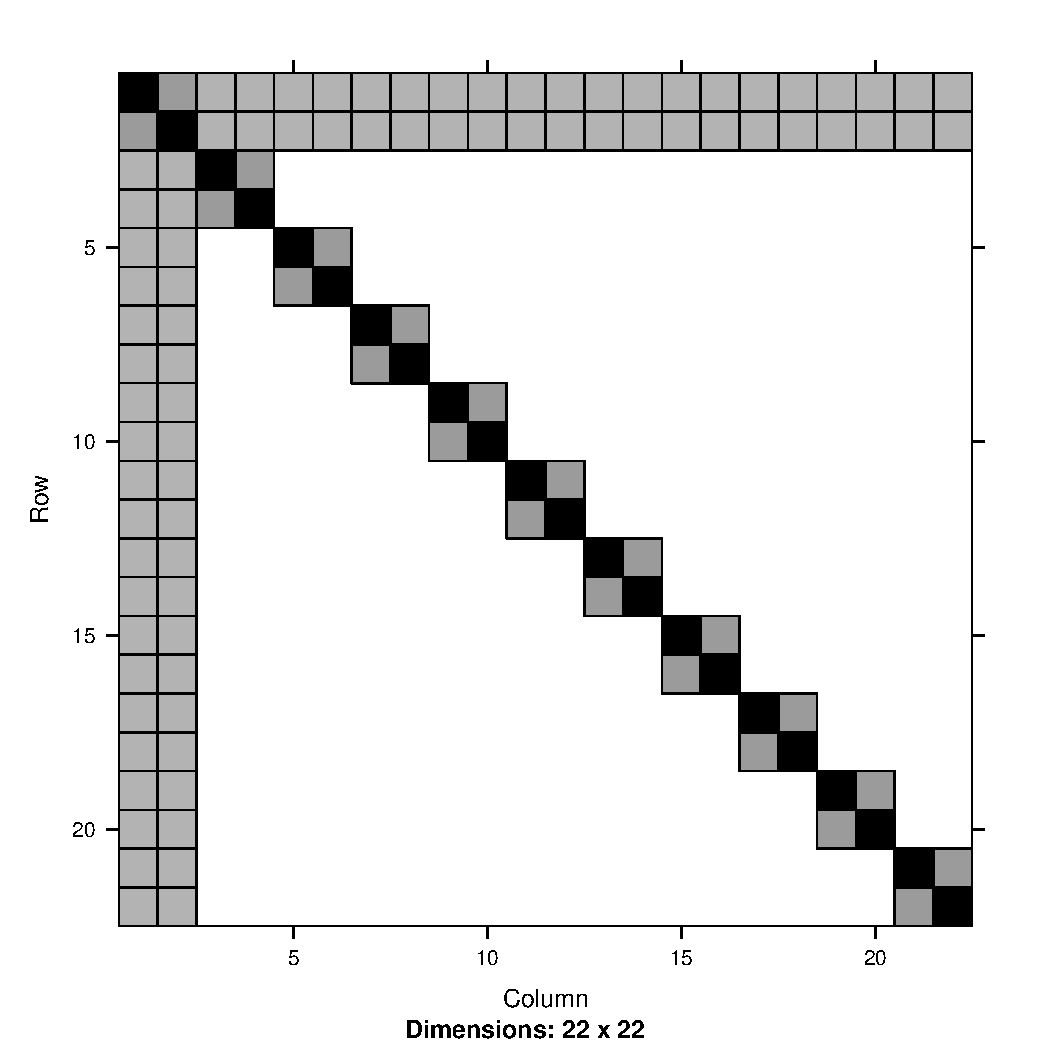
\includegraphics[width=0.95 \textwidth]{mX_mZ_mLambda.pdf}
		\caption{Covariance matrix -- Fixed effects before random effects}
		\label{fig:covfixedrandom}
	\end{figure}
		
	\begin{figure}[p]
		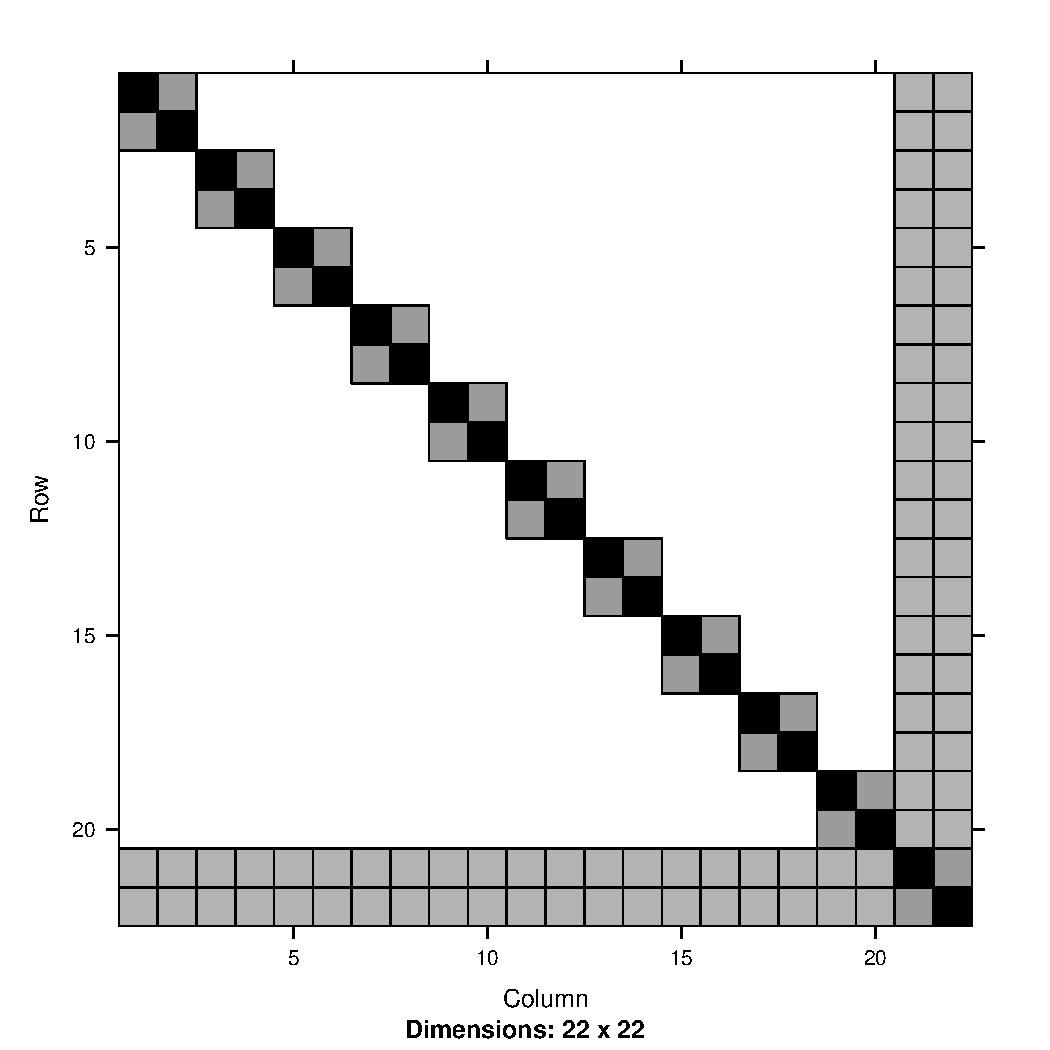
\includegraphics[width=0.95 \textwidth]{mZ_mX_mLambda.pdf}
		\caption{Covariance matrix -- Random effects before fixed effects}
		\label{fig:covrandomfixed}
	\end{figure}
							      				      			      			      			      	
	\begin{figure}[p]
		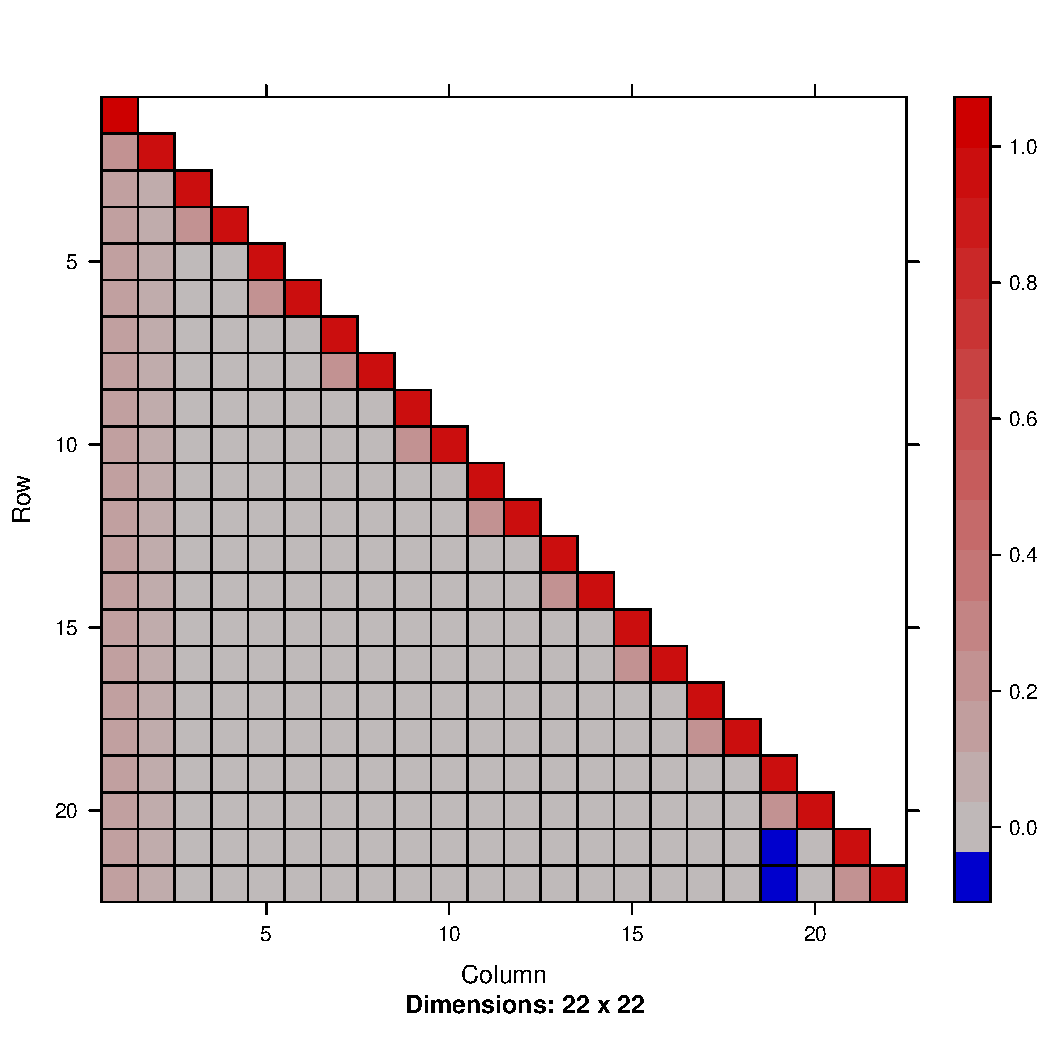
\includegraphics[width=0.95 \textwidth]{mX_mZ_cholesky.pdf}
		\caption{Cholesky factor -- Fixed effects before random effects}
		\label{fig:cholfixedrandom}
	\end{figure}
		
	\begin{figure}[p]
		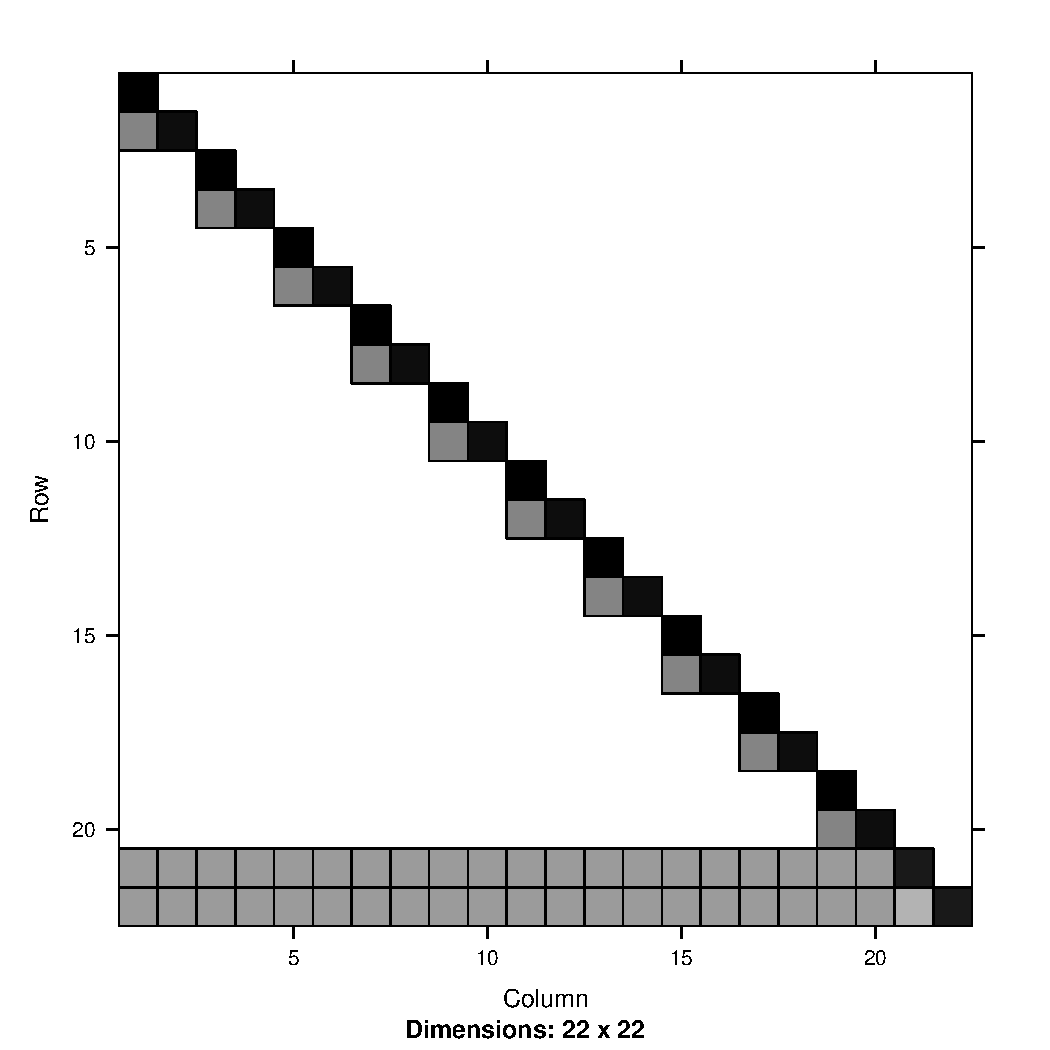
\includegraphics[width=0.95 \textwidth]{mZ_mX_cholesky.pdf}
		\caption{Cholesky factor -- Random effects before fixed effects}
		\label{fig:cholrandomfixed}
	\end{figure}
		
	\subsubsection{Precision parameterisation $\mLambda = (\mR^\top \mR)^{-1}$}
			
	\noindent The second variant of the Gaussian Variational Approximation algorithm is similiar to the first, but
	instead of optimising the Gaussian variational lower bound with respect to $\vmu$ and the Cholesky factor
	$\mR$ of $\mLambda$, we instead optimise the Cholesky factor of the inverse of $\mLambda$ i.e. $\mLambda =
	(\mR \mR^\top)^{-1}$.
	
	The Gaussian variational lower bound in this parameterisation is
	\begin{align*}
		\log \underline{p}(\vmu, \mLambda; \vy) & = \quad \vy\mP\mC \vmu - \vp^\top \exp\{\mC \vmu + \tfrac{1}{2} \text{diag}(\mC \mLambda \mC^\top)\} - \tfrac{1}{2} \vmu^\top \mSigma^{-1} \vmu - \tfrac{1}{2} \tr{(\mSigma^{-1} \mLambda)} \\
		                                        & \quad- \tfrac{p}{2} \log{(2 \pi)} + \tfrac{1}{2} \log{|\mSigma^{-1}|} + \tfrac{p}{2} \log{(2 \pi)} + \tfrac{p}{2} - \log{|\mR|}                                             
	\end{align*}
			
	\noindent The derivative with respect to $\vmu$ is the same as that in the first variant of the algorithm, but 
	as the parameterisation of $\mLambda$ has changed, the  derivative with respect to $\mLambda$ becomes
	\begin{align*}
		\frac{\partial \log \underline{p}(\vmu, \mLambda; \vy)}{\partial \mLambda}
		  & = \hphantom{-}(\mLambda^{-1} + \mH)(-\mLambda \mR \mLambda) \\
		  & = -(\mI + \mH\mLambda)\mR\mLambda                           \\
		  & = - (\mR\mLambda + \mH\mLambda\mR\mLambda)                  
	\end{align*} 
			
	\noindent where $\mH = (\mP \mC)^\top \text{diag}(\exp(\mC \vmu + \frac{1}{2} \mC \mLambda \mC^\top)) \mP \mC - \mSigma^{-1}$.
			
	\subsubsection{GVA fixed point} 	% Fixed point update of \mLambda
	This variant of the algorithm uses Newton-Raphson-like fixed point updates on the Gaussian variational lower
	bound. We optimise the same variational lower bound as in the covariance parameterisation above, using the
	derivatives below. The steps are presented in Algorithm \ref{alg:algorithm_nr} where	
	\begin{align*}
		\frac{\partial \log \underline{p}(\vmu, \mLambda; \vy)}{\partial \vmu}     & = \quad \mC^\top\vp \left \{\vy - \mC\exp(\mC \vmu + \tfrac{1}{2} \text{diag}(\mC \mLambda \mC^\top)) \right \} - \mSigma^{-1} \vmu \text{ and} \\
		\frac{\partial \log \underline{p}(\vmu, \mLambda; \vy)}{\partial \mLambda} & = -\mC^\top \text{diag}(\vp^\top \exp(\mC \vmu +\tfrac{1}{2} \text{diag}(\mC \mLambda \mC^\top))) - \mSigma^{-1}.                             
	\end{align*}
	As this algorithm involves a simple Newton-Raphson style update step, it is computationally simple to
	implement, but potentially unstable as there is no adaptation of step size, as in L-BFGS-B.

	For efficiency, the inversion of $\mLambda$ within the algorithm was implemented using the block inverse 
	formula, where	the matrix was partitioned
	\[
		\mLambda =
		\begin{pmatrix}
			\mLambda_{\vbeta \vbeta} & \mLambda_{\vbeta \vu} \\
			\mLambda_{\vbeta \vu}^\top & \mLambda_{\vu \vu}
		\end{pmatrix}
	\]
	where $\mLambda_{\vbeta \vbeta}$ is the $p \times p$ approximation of the fixed effects covariance, $\mLambda_{\vbeta \vu}$ is the $p \times mb$
	approximation of the covariances between the fixed and random effects and $\mLambda_{\vu \vu}$ is the $mb \times mb$
	approximation of the random effects covariance.

	Sometimes in the course of  executing the algorithm, we observed numerical issues which had to be dealt
	with in order for the algorithm to successfully complete. If the block $\mLambda_{\vu \vu}$ cannot be inverted on an
	iteration, we reverted to $\vmu$ and $\mLambda$ from the previous iteration. If after updating $\vmu$
	any element is NaN, we reverted to the $\vmu$ and $\mLambda$ from the previous iteration. This greatly
	improved the stability of the algorithm.
	
	\begin{algorithm}
		\caption[Algorithm GVA NR]{Iterative scheme for obtaining optimal $\vmu$ and $\mLambda$
			given $\vy$, $\mC$ and $\vp$}
		\label{alg:algorithm_nr}
		\begin{algorithmic}
			\REQUIRE $\frac{\partial \log \underline{p}(\vmu, \mLambda; \vy)}{\partial \vmu} = \mP \mC (\vy - \mC^\top \exp(\mC \vmu + \frac{1}{2} \text{diag}{(\mC \mLambda \mC^\top)})) - \mSigma^{-1} \vmu$.
			% Fit \vmu, \mLambda using Laplace approximation
			\WHILE{the increase in $\log{\underline{p}}(\vmu, \mLambda; \vy)$ is significant}
			% \vmu, \mLambda
			\STATE $\mLambda^{-1} = \left \{ \mP^\top \mC^\top \exp(\mC \vmu + \frac{1}{2} \text{diag}(\mC \mLambda \mC^\top)) \mC \mP \right \}$ \\ [1ex]
			Calculate \STATE $\mLambda \leftarrow \left (\mLambda^{-1} \right )^{-1}$  using the block inverse formula \\ [1ex]
			If $\mLambda_{\vu \vu}$ cannot be inverted in the above calculation, revert to $\vmu$ and $\mLambda$ from the previous iteration \\ [1ex]
			\STATE $\frac{\partial \log \underline{p}(\vmu, \mLambda; \vy)}{\partial \vmu} = -\mC^\top \text{diag}[\vp^\top \exp\{\mC \vmu + \frac{1}{2} \text{diag}(\mC \mLambda \mC^\top)\}] - \mSigma^{-1}$ \\ [1ex]
			\STATE $\vmu \leftarrow \vmu + \mLambda \left \{ \frac{\partial \log \underline{p}(\vmu, \mLambda; \vy)}{\partial \vmu} \right \}$ \\ [1ex]
			If any element of $\vmu$ is NaN, revert to $\vmu$ and $\mLambda$ from the previous iteration
			\ENDWHILE
		\end{algorithmic}
	\end{algorithm}
			
	% Splines
			
	\section{Parameterisations and computational cost of Gaussian Variational Approximation approaches}
	\label{sec:param}
	\subsection{Covariance parameterisation of $\mLambda$}
	
	To ensure symmetry of $\mLambda$, we parameterise the optimisation problem in terms of $\mLambda$'s
	Cholesky factor  $\mLambda = \mR^\top \mR$. We optimise over the space $(\vmu, \overline{\mR})$, where $\vmu
	\in \R^{p + m}b$ and $\overline{\mR}$ is a lower-triangular $(p + mb) \times (p + mb)$ matrix. Then
			
	\begin{equation*}
		\mR_{ij} =
		\begin{cases}
			\exp(\overline{\mR}_{ij}), & i = j             \\
			\overline{\mR}_{ij},       & i > j             \\
			0,                         & \text{otherwise}, 
		\end{cases}
	\end{equation*}
			
	\noindent exponentiating the diagonal to ensure positive-definiteness of $\mR$. We parameterise $\mLambda$
	as $\mLambda = \mR \mR^\top$ so that is is guaranteed to be symmetric, and we only have $p(p-1)/2$ 
	parameters to deal with instead of $p^2$ parameters, some of which are constrained. 
	
	This parameterisation can lead to numeric overflow when the diagonals of $\overline{\mR}$ become moderately
	large, which can lead to singular matrices when attempting to invert $\mLambda$. We dealt with this by
	defining a piecewise function which is exponential for arguments less than $t$, and quadratic for arguments
	greater than or equal to $t$
	$$
	f(r_{ij}) =
	\begin{cases}
		e^{r_{ij}}, r_{ij} < t                   \\
		a r_{ij}^2 + b r_{ij} + c, r_{ij} \geq t 
	\end{cases}
	$$
	and then choosing the co-efficients $a$, $b$ and $c$ such that the function, first and second derivatives would
	agree at $r_{ij} = t$.
	
	To find the co-efficients $a$, $b$ and $c$, we solved the system of equations formed by repeatedly 
	differentiating the quadratic at $r_{ij} =  t$ and equating it with $e^t$
	$$
	\begin{array}{lllll}
		e^t & = & a t^2 & + \quad b t & + \quad c \\
		e^t & = &       & \quad 2a t  & + \quad b \\
		e^t & = &       &             & \quad 2a  \\
	\end{array}
	$$
	to obtain $a = e^t / 2$, $b = (1 - t) e^t$ and $c = \{1 - t^2/2 - (1 - t) t\} e^t$.
	
	We also addressed the overflow problem by working with the Cholesky factorisation of $\mLambda^{-1}$
	rather than $\mLambda$, allowing us to solve a system of equations rather than invert and multiply by a
	matrix, which is also faster and more numerically stable. We use knowledge of the regression  model we are
	fitting to specify a sparse matrix structure, greatly reducing the dimension of   the problem and thus
	improving both computational speed and numeric accuracy.
	
	% \noindent By noticing that the lower rows of the product depend on the higher rows of the Cholesky factor, we
	% observe that by re-ordering the fixed and random effects in $\mLambda$ so that the , we arrive at a covariance structure which is sparse in the first diagonal block. Thus the Cholesky factor of $\mLambda$ that we optimise over is as sparse as possible. This reduces the dimension of the optimisation problem we have to solve from
	% $\BigO(np^2)$ to $\BigO(np)$.
		
	Any symmetric matrix $\mLambda$ can be written as a product of its' Cholesky factors, $\mLambda =
	\mR \mR^\top$ where $\mR$ is lower triangular. $\mR$ is unique if $\mR_{ii} \geq 0$.
		
	\begin{align*}
		&\begin{pmatrix}
		\mR_{11}          & 0                                    & 0                                     \\
		\mR_{21}          & \mR_{22}                             & 0                                     \\
		\mR_{31}          & \mR_{32}                             & \mR_{33}                              
		\end{pmatrix}
		\begin{pmatrix}
		\mR_{11}          & \mR_{21}                             & \mR_{31}                              \\
		0                 & \mR_{22}                             & \mR_{32}                              \\
		0                 & 0                                    & \mR_{33}                              
		\end{pmatrix}
		\\
		=& \begin{pmatrix}
		\mR_{11}^2        &                                      & \text{symmetric}                      \\
		\mR_{21}\mR_{11} & \mR_{21}^2 + \mR_{22}^2 \\
		\mR_{31} \mR_{11} & \mR_{31}\mR_{21} + \mR_{32} \mR_{22} & \mR_{31}^2 + \mR_{32} ^2 + \mR_{33}^2 
		\end{pmatrix}.
	\end{align*}
	
	\noindent We exploit this structure. By interchanging the fixed and random effects in the design matrix $\mC = [\mX \mZ]$ to $\mC = [\mZ \mX]$, and re-ordering the dimensions of $\vmu, \mLambda$ and $\mSigma$ in the same manner, the independence between the
	blocks relating to the random effects in $\mZ$ induce sparsity in the Cholesky factor $\mR$ of
	$\mLambda^{-1}$, as can be seen in Figures \ref{fig:covfixedrandom}, \ref{fig:covrandomfixed},
	\ref{fig:cholfixedrandom} and \ref{fig:cholrandomfixed}. Thus the Gaussian $q(\vnu) \sim \N(\vmu, \mLambda)$ can be optimised over a space of dimension $\frac{1}{2} p (p + 1) + pq + \frac{1}{2} q (q + 1)$ rather than dimension
	$\frac{1}{2} (p + mq) (p + mq + 1)$ as in the dense parameterisation. This leads to subtantial performance gains
	when $m$ is large, as is typically the case in problems of practical importance such as longitudinal or 
	clinical trials with many subjects or the application presented in Section \ref{sec:application}.
			
	By re-ordering the fixed and random effects in $\mLambda$, we end up with a covariance structure which is 
	sparse in the first diagonal block.
	
	\subsection{Precision parameterisation}
	
	We optimise over the space $(\vmu, \overline{\mR})$ as before, but now 
			
	\begin{equation*}
		\mR_{ij} =
		\begin{cases}
			\exp(-\overline{\mR}_{ij}), & i = j             \\
			\overline{\mR}_{ij},        & i > j             \\
			0,                          & \text{otherwise}, 
		\end{cases}
	\end{equation*}
		
	\noindent This new choice of parameterisation allows us to calculate $\frac{1}{2} \text{diag}(\mC \mLambda
	\mC^\top)$ by solving the linear systems $\mR \va = \mC_{i}, i=1, \ldots, n$ for   $\va$ and then calculating
	$\va^\top\va$ where $\mC_{i} = $ the $i$th row of $\mC$, rather than calculating $\text{diag}(\mC \mLambda
	\mC^\top)$ directly.
		
	% TODO: We fixed this using safe-exp
	The implementation of these algorithms was not without its' challenges, chiefly numerical issues encountered during testing and verification of the accuracy of the model fitting. Using the exponential function to parameterise the main diagonal coupled with L-BFGS-B's unconstrained line search and \texttt{optim()}'s lack of robustness to infinities lead to many overflow problems which may have been lessened or dealt with entirely by using a function with a less aggressive growth rate, such as an appropriate piecewise quadratic.
		
	The main computational cost is the evaluation of the variational lower bound and its' derivatives. By
	virtue of their dimension, the expressions involving $\mLambda$ dominate the computational cost. The key
	term is $\frac{1}{2} \diag(\mC \mLambda \mC^\top)$. This can be naively calculate by ignoring the
	symmetry in the expression and simply calculating the product $\mC \mLambda \mC^\top$, taking $2 n
	\times (p + m b)^2$ floating point operations, and retaining the diagonal entries of the result. This is
	obviously wasteful, as the off--diagonal entries of the resulting product that has just been computed
	are immediately discarded.
		
	By parameterising $\mLambda$ in terms of its' Cholesky factors and realising that
		
	\[
		\mC \mLambda \mC^\top = \mC \mR \mR^\top \mC^\top
	\]
		
	\noindent and that
		
	\[
		\diag(\mC \mLambda \mC^\top)_{ii} = \mC_{i .} \mR \mR^\top \mC_{i .}^\top, 1 \leq i \leq n
	\]
		
	\noindent we can calculate the products $\mC_{i .} \mR, 1 \leq i \leq n$, using $n \times \frac{1}{2}(p + m
	b)(p + m b   + 1)$ floating point operations, and storing the results of the $i$th product in the $i$th
	element of the   vector $\va$ and then calculate $\diag(\mC \mLambda \mC^\top) = \va^\top \va$.
		
	Moreover, mixed models typically have sparse design matrices, allowing us to encode $\mR$ as a sparse matrix, and	further reduce   this depending on the model. For example, in the random intercept case, only the diagonals of the random effects block need to be non-zero, and hence the above expression can be calculated in
	$\BigO(n)$ floating point operations.
		
	% $\log |\mR|$ can be calculated using only $p + m b$ floating point operations, as $\mR$ is lower triangular.
		
	For the precision parameterisation, we observe that in this parameterisation
	\[
		\diag(\mC \mLambda \mC^\top)_{ii} = \mC_{i .} \mR^{-\top} \mR^{-1} \mC_{i .}^\top, 1 \leq i \leq n,
	\]
		
	\noindent and so by solving $\mR \va = \mC_{i .}^\top$ for $\va$ for all $i$ at a cost of $n \times
	\frac{1}{2} (p + m b) (p + m b + 1)$ floating point operations, and then calculating
	\[
		\diag(\mC \mLambda \mC^\top)_{ii} = \va^\top \va, 1 \leq i \leq n,
	\]
		
	\noindent we can then calculate $\diag(\mC \mLambda \mC^\top)$.
		
	As above, by using our knowledge of the model being fit we can encode $\mR$ sparsely to decrease
	the required   computation still further. In the random intercept model case, the computational cost will drop
	to   $n \times [m + \frac{1}{2} p (p + 1) + p \times m b]$.
				
			\section{Numerical results}
			\label{sec:results}
					
			The accuracy of each model fitting algorithms presented in Section \ref{sec:gaussian} was assessed by
			comparing the approximating distribution of each parameter with the posterior distribution of Monte Carlo
			Markov Chain samples of that parameter. 1 million Monte Carlo Markov Chain samples were generated using Stan.
			The accuracy of examples of random intercept, random slope and spline models were evaluated using this method.
					
			\subsection{Simulated data}
					
			For each of these simulations, the model is as presented in Section \ref{sec:model}.
					
			Several common application scenarios were simulated and their accuracy evaluated. A random intercept model was simulated with $\vbeta = (2, 1)^\top$, $\rho = 0.5$, $m = 20$, $n_i = 10$ and $b = 1$. The results are
			presented in Table \ref{tab:accuracy_int}. A random slope model was simulated with $\vbeta = (2, 1)^\top$,
			$\rho = 0.5$, $m = 20$, $n_i = 10$ and $b = 2$. The results are presented in Table \ref{tab:accuracy_slope}.
			Spline model was fit to a data set generated from the function $3 + 3 \sin{(\pi x)}$ on the interval $[-1,
			1]$. The resulting model fits are presented in Figure \ref{fig:spline}.
					
			To assess the speed of each approach, a test case was constructed of a random slope model with $m=50$ groups,	each containing $n_i = 100$ individuals. A model was then fit to this data set ten times using each algorithm, and the results averaged. They are presented in Table \ref{tab:application_slope_speed}.

			\begin{table}
				\caption{Table of results - Speed}
				\label{tab:application_slope_speed}
				\begin{tabular}{|l|rr|}
					\hline
					Algorithm & Mean (seconds) & Standard deviation (seconds) \\
					\hline
					Laplace's method & 0.37 & 0.07 \\
					GVA covariance parameterisation & 2.04 & 1.24 \\
					% Why is this slower?
					GVA inverse parameterisation & 0.38 & 0.66 \\
					GVA fixed point & 0.05 & 0.07 \\
					\hline
				\end{tabular}
			\end{table}

			% The stability of the algorithms was confirmed by running them on 10,000 different data sets that were randomly
			% generated after having initialised the random number generator with different seeds.
					
			Median accuracy of the algorithms was assessed by running them on 100 randomly generated data sets. The	results are presented in Figure \ref{fig:median_accuracy_intercept} and Figure
			\ref{fig:median_accuracy_slope}.
					
			% Figure: Median accuracy graph intercept
			\begin{figure}
				\begin{center}
					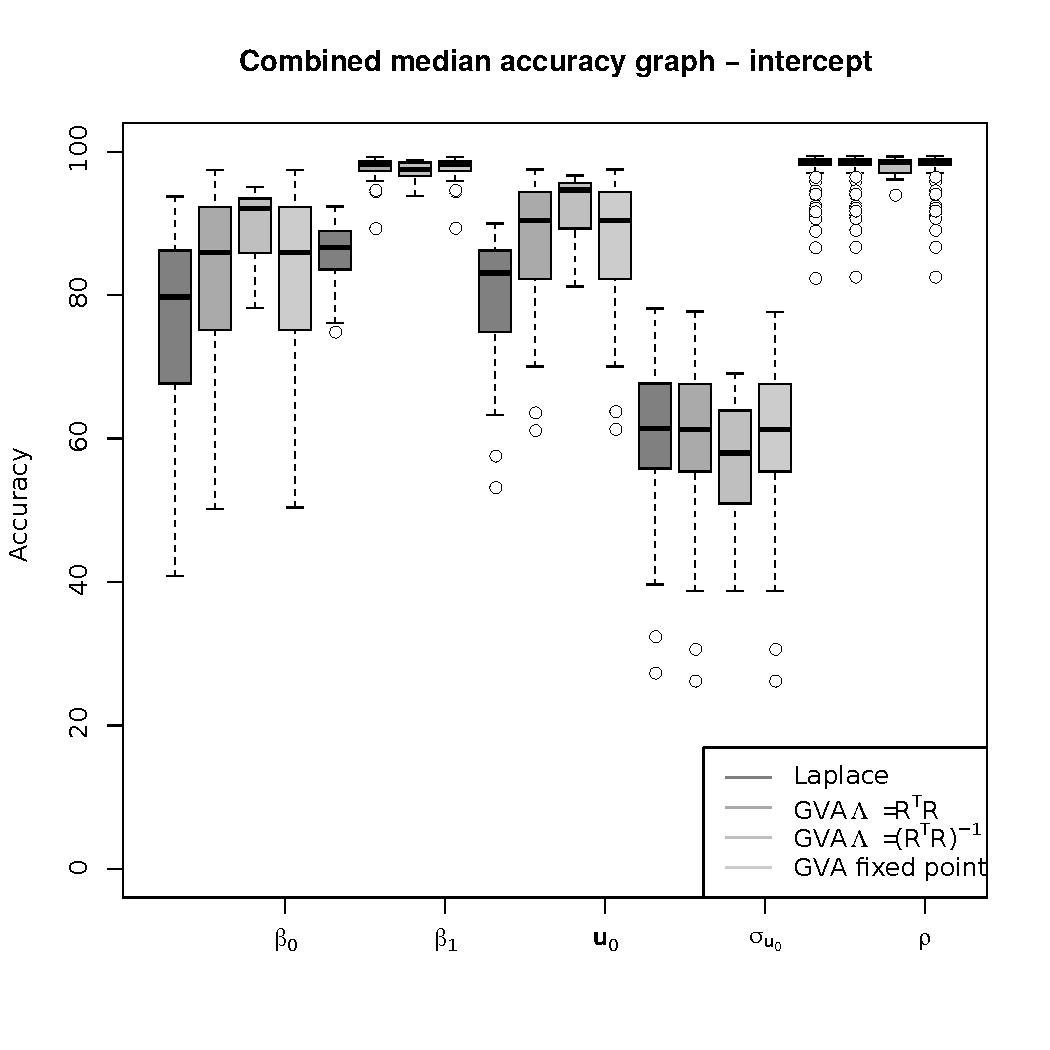
\includegraphics[width=0.95\textwidth, height=100mm]{code/results/median_accuracy_combined_intercept.pdf}
					\caption{Median accuracy of random intercept}
					\label{fig:median_accuracy_intercept}
				\end{center}
			\end{figure}
					
			% Figure: Median accuracy graph slope
			\begin{figure}
				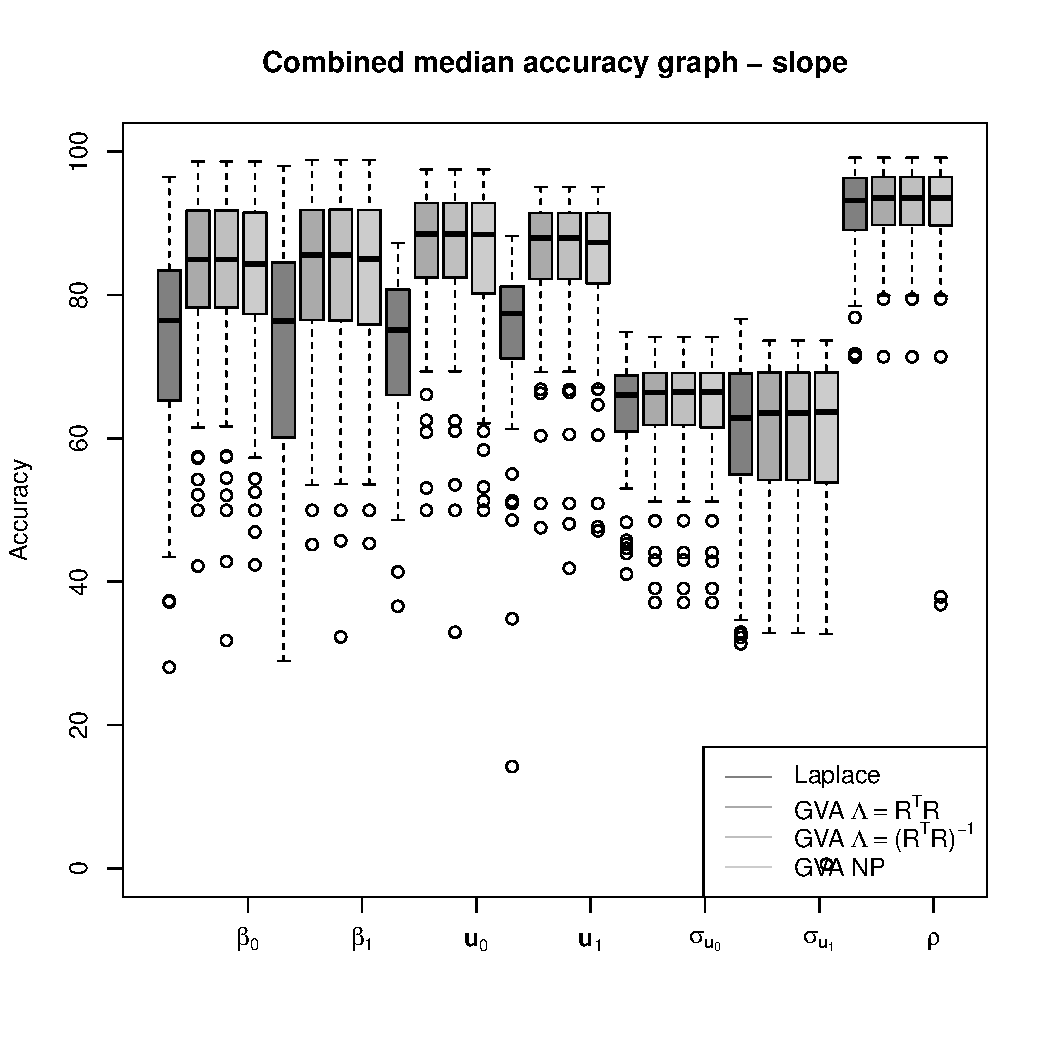
\includegraphics[width=0.95\textwidth, height=120mm]{code/results/median_accuracy_combined_slope.pdf}
				\caption{Median accuracy of slope}
				\label{fig:median_accuracy_slope}
			\end{figure}
					
			% Table of accuracy results - intercept model
			\begin{table}
				\caption{Table of accuracy - Random intercept model}
				\label{tab:accuracy_int}
				\begin{tabular}{|l|rrrr|}
					\hline
					                   & Laplace's Method & GVA $(\mLambda = \mR \mR^\top)$ & GVA NP $(\mLambda = (\mR \mR^\top)^{-1})$ & GVA FP \\
					\hline
					$\vbeta_1$         & $85\%$           & $90\%$                          & $91\%$                                    & $90\%$ \\ 
					$\vbeta_2$         & $76\%$           & $98\%$                          & $99\%$                                    & $99\%$ \\ 
					Mean of $\vu$      & $81\%$           & $94\%$                          & $94\%$                                    & $94\%$ \\
					$\sigma^2_{\vu_1}$ & $66\%$           & $66\%$                          & $66\%$                                    & $66\%$ \\ 
					$\rho$             & $99\%$           & $99\%$                          & $99\%$                                    & $99\%$ \\ 
					\hline
				\end{tabular}
			\end{table}
					
			\begin{table}
				\caption{Table of accuracy - Random slope model}
				\label{tab:accuracy_slope}
				\begin{tabular}{|l|rrrr|}
					\hline
					                   & Laplace's Method & GVA $(\mLambda = \mR \mR^\top)$ & GVA $(\mLambda = (\mR \mR^\top)^{-1})$ & GVA FP \\
					\hline
					$\vbeta_1$         & 67\%             & 88\%                            & 88\%                                   & 88\%   \\
					$\vbeta_2$         & 70\%             & 89\%                            & 88\%                                   & 89\%   \\
					Mean of $\vu$      & 70\%             & 91\%                            & 91\%                                   & 91\%   \\
					$\sigma^2_{\vu_1}$ & 71\%             & 73\%                            & 73\%                                   & 73\%   \\
					$\sigma^2_{\vu_2}$ & 68\%             & 69\%                            & 69\%                                   & 69\%   \\
					$\rho$             & 91\%             & 90\%                            & 90\%                                   & 90\%   \\
					\hline
				\end{tabular}
			\end{table}
					
			% \begin{table}
			% \caption{Table of accuracy - Splines}
			% \label{tab:accuracy_spline}
			% \begin{tabular}{|l|l|}
			% \hline
			% Approximation & Accuracy \\
			% \hline
			% Laplace's Method & 0.969 \\
			% GVA & 0.969 \\
			% GVA NP & 0.969 \\
			% GVA NR & 0.969 \\
			% \hline
			% \end{tabular}
			% \end{table}
					
			\begin{figure}
				\label{fig:spline}
				\caption{Comparison of VB and MCMC spline fits with the true function}
				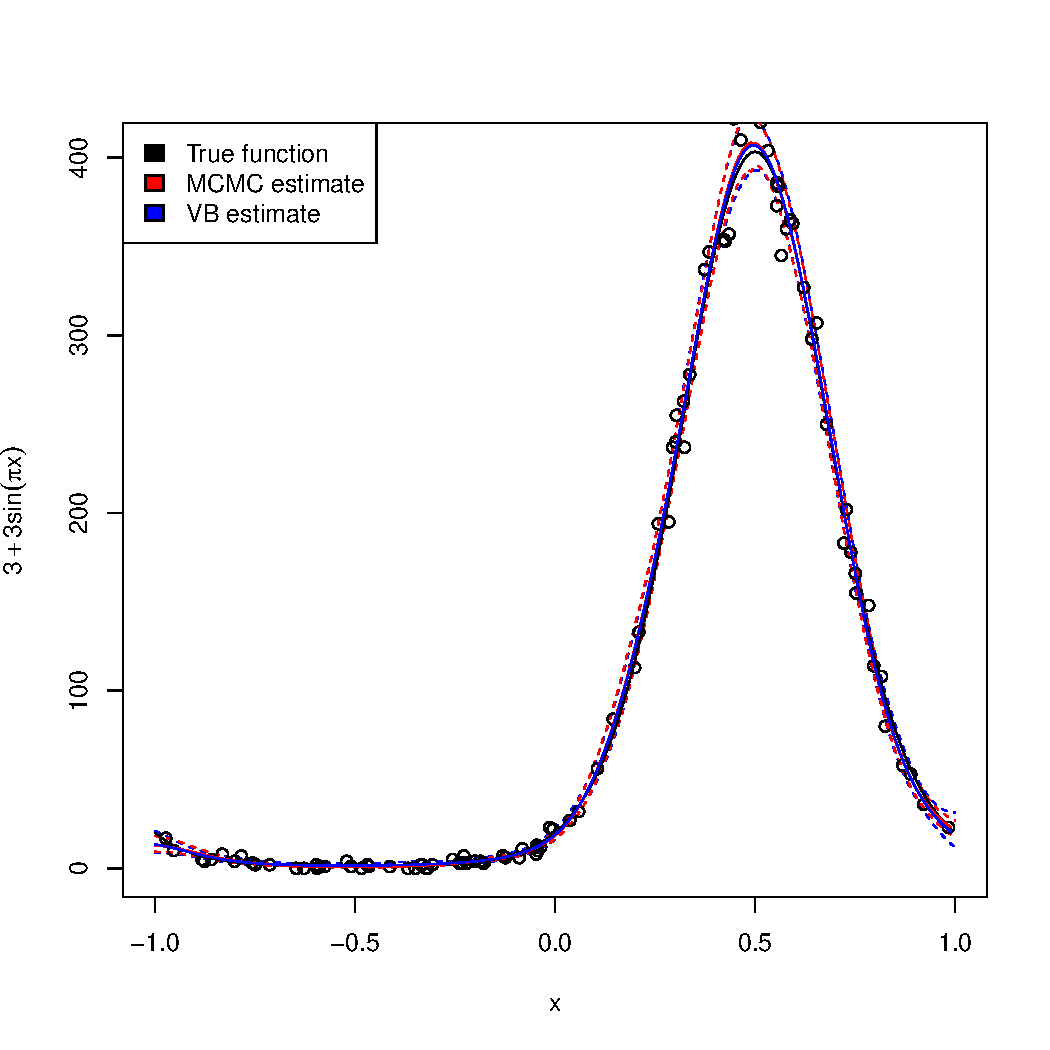
\includegraphics[width=0.95 \textwidth, height=100mm]{code/results/accuracy_plots_spline_gva2.pdf}
			\end{figure}
					
			% Graphs - exactly what sort of graphs do we need?
			% Median accuracy
			% Increase in lower bound
			% MCMC posterior, with approximating posterior for at least one or two of the
			% key parameters, such as, say, vbeta[2]
					
			\subsection{Numerical stability of the parameterisation}
			
			In the process of performing numerical experiments, we discovered that our model fitting software was 
			prone to numeric overflow due to the log link in our model and the exponentiation of the diagonals of the
			Cholesky factors in the covariance parameterisation of the Gaussian Variational Approximation of $\vnu$.
			
			We dealt with this difficulty by developing a 'safe exponential' parameterisation for the diagonals of the
			Cholesky factors. The parameterisation is exponential up to a threshold $t$, and then quadratic beyond that
			threshold.
			
			The stability of this scheme was tested by calculating the accuracy of the approximations fit with a range
			of safe exponential thresholds, the results of which are presented in Figure \ref{fig:stability_accuracy}.
			The variational approximation was found to be stable, with the accuracy largely insensitive to the choice of
			threshold.
			
			\begin{figure}
				\includegraphics[width=0.95 \textwidth]{code/stability_intercept.pdf}
				\label{fig:stability_accuracy}
				\caption{Accuracy of approximation of parameters versus the safe exponential threshold}
			\end{figure}
			
			We repeated our numerical experiments with the new parameterisation, varying the threshold within reasonable
			bounds and found that the numerical experiments no longer resulted in overflow, and that the numerical accuracy
			of the approximation was still very good.
			
			The stability of the GVA algorithm with the parameterisation $\mLambda = (\mR^\top \mR)^{-1}$ depends on the
			threshold chosen for the safe exponential function. When the threshold is set to $2$, the algorithm is stable
			for all starting points within the grid except $6$. When the threshold is set to $\infty$, equivalent to using
			the naive $\exp$ parameterisation, the algorithm encounters numerical errors for every starting point on the 
			grid.
				
			\subsection{Stability of the GVA precision parameterisation algorithm for different starting points}
					
			The numerical stability of each fitting algorithm in Section \ref{sec:gaussian} was assessed by initialising
			each algorithm from a range of different starting points. Errors due to numerical instability and the fitted
			$\vmu$ were recorded for each starting point.
					
			A data set of 100 individuals in ten groups ($m=10$) was generated from a model with a fixed intercept and
			slope, and a random intercept. $\vmu$ was initialised from a grid of points on the interval $[-4.5, 5]$ for
			intercept and slope, spaced $0.1$ apart. The error counts are presented in Table
			\ref{tab:stability_results}. Plots of the starting locations which resulted in numerical errors when the
			fitting algorithm was run are presented in \ref{fig:stability_locations_gva}.
					
			\begin{table}
				\begin{tabular}{|l|r|}
					\hline
					Algorithm                            & Error count \\
					\hline
					Laplace's algorithm                  & 12          \\
					GVA $\mLambda = \mR^\top \mR$        & 1,306       \\
					GVA $\mLambda = (\mR^\top \mR)^{-1}$ & 6           \\
					GVA NR fixed point                   & 992         \\
					\hline
				\end{tabular}
				\caption{Count of numerical errors for each algorithm during stability tests}
				\label{tab:stability_results}
			\end{table}

			The GVA algorithm with the $\mLambda = (\mR \mR^\top)^{-1}$ parameterisation was less prone to
			instability due to starting point when the safe exponential parameterisation was used then when it was
			not used, as can be seen from Figure \ref{fig:stability_locations_gva}. % FIXME: Add error counts
					
			\begin{figure}
				\includegraphics[width=0.95 \textwidth]{code/safe_exp_stability.pdf}
				\includegraphics[width=0.95 \textwidth]{code/no_safe_exp_stability.pdf}
				\label{fig:stability_locations_gva}
				\caption{Starting locations which caused the GVA fitting algorithm to fail with numeric errors. The true model had fixed parameters $\vbeta = (2, 1)^\top$ and random intercepts. There were ten groups in the
					hierarchical model each	with ten individuals $(m=10, n_i=10)$}
			\end{figure}

			\subsection{Stability of the GVA fixed point algorithm for different starting points}

			The naive fixed point algorithm was extremely unstable for many starting points, as can be seen from
			Figure \ref{fig:stability_locations_nr}. The variant of the algorithm which checked whether the
			inversion of the $\mLambda_{\vu \vu}$ block of $\mLambda$ was performed successfully was much more
			stable, and did not suffer from any numeric errors at all over the range of starting points we tested.
			The algorithm is able to abort safely, and allow the Variational Bayes algorithm to update the other
			parameters before trying to fit the Gaussian component of the model again until the correct parameters
			are accurately estimated.

			\begin{figure}
				\includegraphics[width=0.95 \textwidth]{code/local_solutions_gva_nr_error_locations_no_protections.pdf}
				\label{fig:stability_locations_nr}
				\caption{Starting locations which caused the NR fitting algorithm to fail with numeric errors. The true model 						had fixed parameters $\vbeta = (2, 1)^\top$ and random intercepts. There were ten groups in the
					hierarchical model each	with ten individuals $(m=10, n_i=10)$}
			\end{figure}
			
			\section{Application}
			\label{sec:application}
			
			\subsection{Poisson example without zero-inflated component -- Police stops}
			The data set used for this example was the police stop example from Chapter 15 of \citep{Gelman2007}.
			The model fit was
			\begin{align*}
				\vy_{ep}        & \sim \text{Poisson}(n_{ep} e^{\beta_0 + \beta_e \text{ethnicity}_e + \alpha_{c} \text{crime} + \vu_p}), \\
				\valpha				& \sim \N(0, \sigma_\valpha^2),	\\
				\vbeta        & \sim \N(0, \sigma_\vbeta^2), \text{ and }\\
				\vu_p         & \sim \N(0, \sigma_\vu^2)
			\end{align*}
			where $p$ is the $p$-th precinct, and $e$ is the $e$-th ethnicity (blacks, hispanics or whites), and $c$ is
			the $c$-th category of crime (violent crimes, weapons crimes, propery crimes, drug crimes). The random 
			intercepts $u_p$ allow for variation in the base rates of stops across precincts,
			the co-efficients $\beta_j$ measure the effect of ethnicity on the rate of police stops and
			the co-efficients $\alpha_k$ measure the effect of each type of crime on the rate.
			The model finds the relationship between the number of police stops in each precinct and 
			ethnicity	for each type of crime.
			
			The model was fit using the GVA algorithm with the $\mLambda = (\mR^\top \mR)^{-1}$ parameterisation, using
			the prior $a_\rho = 3$, $b_\rho = 1$ on $\rho$. Accuracy of the approximation was assessed by comparing the
			fitted distribution for each parameter to a kernel density estimate of the parameter's distribution from
			1 million samples from the equivalent model fitted using Stan. The results are presented in Table
			\ref{tab:application_police_stops}. Figure \ref{fig:police_stops}
			
			\begin{figure}
			\includegraphics[width=0.95 \textwidth]{code/results/accuracy_plots_application2_GVA_inv_par-highlights-nup.pdf}
			\caption{Accuracy of parameter estimates for police stops}
			\label{fig:police_stops}
			\end{figure}

			% Table of results
			\begin{table}
				\caption{Table of results - Police stops}
				\label{tab:application_police_stops}
				\begin{tabular}{|l|rrrr|}
					\hline
					Covariate                     & Posterior Mean & Lower 95\% CI & Upper 95\% CI & Accuracy \\
					\hline
					Intercept [African-Americans] & 4.04          & 3.98           & 4.07          & 82.4\%   \\
					$\beta_2$ [hispanics]         & -0.45         & -0.46          & -0.43         & 98.1\%   \\
					$\beta_3$ [whites]            & -1.38         & -1.40          & -1.37         & 98.5\%   \\
					$\alpha_1$ [weapons crimes]   & 0.58          & 0.57           & 0.59          & 89.2\%   \\
					$\alpha_2$ [property crimes]  & -0.19         & -0.21          & -0.17         & 92.2\%   \\
					$\alpha_3$ [drug crimes]      & -0.750        & -0.77          & -0.73         & 94.9\%   \\
					Random intercept              & 1.321         & -0.190         & 2.202         & 86.7\%   \\
					$\sigma^2_{\vu}$              & 8.57          & 1.02           & 24.35         & 49\%     \\
					\hline
				\end{tabular}
			\end{table}
			
			% Table of speeds
			\begin{table}
				\begin{tabular}{|ll|}
					\hline
					Algorithm & Time  in seconds \\
					\hline
					Laplace & 0.24 \\
					GVA covariance parameterisation & 6.02 \\
					GVA inverse paramaterisation & 3.92 \\
					GVA fixed point & 0.18 \\
					\hline
				\end{tabular}
				\caption{Table of speeds - Police stops}
				\label{tab:police_stop_speeds}
			\end{table}
			
			% TODO: You need to describe the data set and the model.
			\subsection{Zero--inflated example -- Cockroaches in Apartments data set from Gelman}
			The model described in this section was fit
			 to the cockroach data set from \S 6.7 of \citep{Gelman2007}, taken from a study
			on the effect of integrated pest management in controlling cockroach levels in urban apartments. The data
			set contains data on 160 treatment and 104 control apartments, along with the response $y_i$ in each
			apartment of the number of cockroaches caught in a set of traps. The apartments had the traps deployed for
			different numbers of days, referred to as trap days, which was handled by using a log offset
			\citep{Agresti2002}. The predictors in the data set included the pre-treatment roach level, a treatment
			indicator, the time of the observation and an indicator for whether the apartment is in a senior building
			restricted to the elderly.
					
			In the example application presented in this paper, the zero component represents an apartment completely free of roaches, while the non-zero component represents an apartment where roaches have been able to live and reproduce, possibly in spite of pest control treatment aimed at preventing them from doing so.

			The model fit was
			\begin{align*}
				y_i &= \begin{cases}
				0 \phantom{-} \text{if} \phantom{-} R_i = 0 \\
				\text{Poisson}(e^{\mX_i \vbeta + \mZ_i \vu}) \phantom{-} \text{if} \phantom{-} R_i = 1,
				\end{cases} \\
				R_i &\sim \text{Bernoulli}(\rho), \\
				\rho &\sim \text{Beta}(a, b), \\
				\vbeta &\sim \text{N}(\vzero, \sigma^2_\vbeta \mI), \\
				\vu &\sim \text{N}(\vzero, \mSigma), \text{and} \\
				\mSigma &\sim \text{Inverse-Wishart}(\mPsi, v)
			\end{align*}
			with prior parameters $a = 1$, $b = 1$, $\sigma^2_\vbeta = 10^5$, $\mPsi = 10^{-5} \mI$ and $v = 2$.
			These priors were chosen to be vaguely informative for the variance components and a uniform prior for
			the zero-inflation proportion latent variable $\rho$. The fixed effects covariates included in the
			model were time in days and time in days $\times$ pest control treatment. A random intercept to account
			for variation between the apartment buildings was included.
					
			The GVA algorithm with the $\mLambda = (\mR^\top \mR)^{-1}$ parameterisation was used to fit a random
			intercept model to the Roaches data set provided by Andrew Gelman. The fitted co-efficients and accuracy
			results are presented in Table \ref{tab:application_roaches}.
					
			%       lci  uci
			% 1  3.179 3.157 3.201
			% 2 -0.046 -0.053 -0.039
			% 3 -0.420 -0.434 -0.406
			% 1 -0.976 -1.015 -0.936
			% 2 -0.309 -0.323 -0.295
			% 3 -0.947 -0.963 -0.930
			% 4 -2.129 -2.384 -1.874
			% 5 -3.230 -3.490 -2.970
			% 6 -3.099 -3.404 -2.794
			% 7 -1.290 -1.326 -1.255
			% 8 -0.956 -0.991 -0.921
			% 9 -2.404 -2.600 -2.209
			% 10 -1.076 -1.123 -1.029
			% 11 -1.079 -1.107 -1.052
			% 12 -1.681 -1.737 -1.624
					
			%> round(cbind(fit1$vmu, lci, uci), 3)
			% fit1$a_rho
			% [1] 377.2375
			% > fit1$b_rho
			% [1] 152.7625
					
			\begin{table}
				\begin{tabular}{|l|rrrr|}
					\hline
					Covariate          & Posterior Mean & Lower 95\% CI & Upper 95\% CI & Accuracy \\
					\hline
					Intercept          & 3.42						& 3.2 					& 3.65          & 95\%     \\
					Time               & $-$0.14        & $-$0.05       & $-$0.02       & 96\%     \\
					Time:Treatment     & $-$0.31        & $-$0.43       & $-$0.14       & 96\%     \\
					Random intercept   & $-$1.60        & $-$1.71       & $-$1.49       & 90\%     \\
					$\sigma^2_{\vu_1}$ & 3.29           & 2.02          & 8.48          & 63\%     \\
					$\rho$             & 0.51           & 0.50          & 0.55          & 62\%     \\
					\hline
				\end{tabular}
				\caption{The posterior means, 95\% confidence intervals and accuracy of the fixed and random
									effects, $\sigma_{\vu_1}^2$ and $\rho$ for the Roach model.}
				\label{tab:application_roaches}
			\end{table}

			\begin{table}
				\begin{tabular}{|lr|}
				\hline
				Algorithm & Time in seconds \\
				\hline
				Laplace & 0.49 \\
				GVA & 1.08 \\
				GVA inv. param & 0.81 \\
				GVA fixed point & 0.11 \\
				\hline
				\end{tabular}
				\label{tab:application_roaches_runtime}
				\caption{The runtimes in seconds for fitting algoritms when fitting the roach model.}
			\end{table}
					
			\begin{figure}
				\centering
				% \includepdf[width=75mm,height=75mm,pages={1,2,3,16},nup=2x2]{code/results/accuracy_plots_application_GVA2.pdf}
				\begin{tabular}{@{}c@{\hspace{.5cm}}c@{}}
				\includegraphics[width=0.95 \textwidth]{code/results/accuracy_plots_application_GVA_inv_param-highlights-nup.pdf}
				\end{tabular}
				\caption{Accuracy graphs for roach model}
				\label{fig:accuracy_roach}
			\end{figure}
					
			\subsection{Example - Biochemists}
			The model described in this section was fit to the biochemistry data set analysed by
			\cite{10.2307/2579146}. The sample was taken from 915 biochemistry graduate students. The outcome
			$\vy_i$ is the number of articles published in the last three years of the PhD. The covariates were the
			gender of the student, coded $1$ for female and $0$ for male, the marital status of the student ($1$ for
			married, $0$ for unmarried), the number of children under age six and the prestige of the PhD program.

			In this example application, the zero component represents the number of biochemists who did not publish
			any articles during the last three years of their PhD. Examination of the data reveals that this number
			is higher than would be expected if the data followed a purely Poisson distribution -- 30\% of
			biochemistry graduate students published no articles in their final years whereas a Poisson distribution
			would predict only 18\%. This justifies our choice of model.

			The model fit was
			\[
				y_i = \begin{cases}
				\begin{array}{ll}
				0 &\phantom{-} \text{if} \phantom{-} R_i = 0, \\
				\text{Poisson}(e^{\vbeta_1 + \vbeta_2 \text{female} + \vbeta_3 \text{married} + \vbeta_4 \text{children under age 6} + \vbeta_5 \text{PhD}}) &\phantom{-} \text{if} \phantom{-} R_i = 1,
				\end{array}
				\end{cases}
			\]


			\noindent with priors
			\begin{align*}
			R_i &\sim \text{Bernoulli}(\rho), \\
			\rho &\sim \text{Beta}(A, B), \text { and } \\
			\vbeta &\sim \text{N}(0, \sigma_\vbeta^2 \mI)
			\end{align*}

			\noindent with $A=1$, $B=1$ and $\sigma_\vbeta^2 = 10,000$. The model was fit using the GVA inverse parameterisation algorithm. The resulting model fit is presented in Table \ref{tab:biochemists_results}
			The accuracy of the parameter estimates is presented in Figure
			\ref{fig:biochemists}. As this is a fixed effects model with a large number of samples relative to the
			number of parameters being fit, we are able to estimate all of the parameters with great accuracy.

			\begin{figure}
			\includegraphics[width=0.95 \textwidth]{code/results/accuracy_plots_application_biochemists_GVA_inv_param-nup.pdf}
			\label{fig:biochemists}
			\caption{Accuracy of the approximations of the parameters fit to the biochemists data}
			\end{figure}

			\begin{table}
				\begin{tabular}{|l|rrrr|}
					\hline
					Covariate          & Posterior Mean & Lower 95\% CI & Upper 95\% CI & Accuracy \\
					\hline
					Intercept & 0.86 & 0.65 & 1.06 &  95.17\% \\
					Female & -0.18 & -0.29 & -0.08 &  95.05\% \\
					Married & 0.06 & -0.05 & 0.18 & 95.66\% \\
					Children under age 6 & -0.08 & -0.15 & -0.01 & 96.71\% \\
					PhD & 0.03 & -0.02 & -0.01 & 96.91\% \\
					\hline
				\end{tabular}			
				\label{tab:biochemists_results}
				\caption{The posterior means, 95\% confidence intervals and accuracy of the fixed effects for the 
									Biochemists model.}
			\end{table}

			\begin{table}
				\begin{tabular}{|l|r|}
				\hline
				Algorithm & Time in seconds \\
				\hline
				Laplace & 1.01 \\
				GVA & 0.96 \\
				GVA inv. param & 0.68 \\
				GVA fixed point & 0.41 \\
				\hline
				\end{tabular}
				\label{tab:biochemists_runtime}
				\caption{The runtimes in seconds for fitting algoritms when fitting the Biochemists model.}
			\end{table}
			
			\subsection{Example - Owls}
			The model described in this section was fit to the Owls data set from taken from \cite{zuur_mixed_2009}.
			The sample was 599 observations of owls grouped across 25 nests.The fixed covariates
			fit in the model were food treatment (Deprived or Satiated) and arrival time, a continuous covariate.
			The variation between the 25 different nests sampled from was modelled by a random intercept
			$\vu$.

			The model fit was
			\[
			y_i = R_i e^{\vbeta_2 \text{Food Treatment = Satiated} + \vbeta_3 \text{Arrival Time} + u_n}
			\]
			where $n$ is the $n$-th nest, with priors
			\begin{align*}
			R_i &\sim \text{Bernoulli}(\rho), \\
			\rho &\sim \text{Beta}(A, B), \\
			\vbeta &\sim \text{N}(\vzero, \sigma_\vbeta^2 \mI), \\
			\vu &\sim \text{N}(0, \sigma_\vu^2), \text { and } \\
			\sigma_\vu^2 &\sim \text{Inverse-Gamma}(s, t).
			\end{align*}
			where $\sigma_\vbeta^2=10,000$, $A=1$, $B=1$, $s=10^{-2}$ and $r=10^{-2}$.

			The model was fit using the GVA inverse parameterisation algorithm. The accuracy of the parameter
			estimates is shown in Figure \ref{fig:owls}. The variance component
			The runtime of the algorithms is shown in Table
			\ref{tab:owls_times}. We draw attention to the difference in run-times between the covariance and
			inverse parameterisations -- the inverse parameterisation is 

			\begin{figure}
				\includegraphics[width=0.95 \textwidth]{code/results/accuracy_plots_application_owls_GVA_inv_param-highlights-nup.pdf}
				\caption{Accuracy of the approximations of the parameters fit to the Owls data}
				\label{fig:owls}
			\end{figure}

			\begin{table}
				\begin{tabular}{|l|rrrr|}
					\hline
					Covariate          & Posterior Mean & Lower 95\% CI & Upper 95\% CI & Accuracy \\
					\hline
					Satiated & -0.217 & -0.212 & -0.214 & 97\% \\
					Arrival Time & -0.070 & -0.070 & -0.070 & 73\% \\
					Random intercept (nest) & 0.338 & -5.283 & 5.959 & 84\% \\
					$\sigma_{\vu_1}^2$ & 7.90 & 3.213 & 468.123 & 94\% \\
					$\rho$ & 0.739 & 0.703 & 0.774 & 99\% \\
					\hline
				\end{tabular}			
				\label{tab:owls_results}
				\caption{The posterior means, 95\% confidence intervals and accuracy of the fixed and random
									effects, $\sigma_{\vu_1}^2$ and $\rho$ for the Owls model.}
			\end{table}

			\begin{table}
				\begin{tabular}{|l|r|}
				\hline
				Algorithm & Time in seconds \\
				\hline
				Laplace & 0.71 \\
				GVA covariance parameterisation & 5.66 \\
				GVA inverse parameterisation & 1.88 \\
				GVA fixed point & 0.18 \\
				\hline
				\end{tabular}
				\caption{The runtimes of the fitting algorithms for the Owls model in seconds.}
				\label{tab:owls_times}
			\end{table}

			\section{Discussion}
			\label{sec:discussion}
					
			We have described a Variational Bayes approximation to Zero-Inflated Poisson regression models which allows
			such models to be fit with considerable generality. We have also devised and extensively tested a number of
			alternative approaches for fitting such models, and extended one of these alternative approaches with a new
			parameterisation. Using MCMC methods as the gold standard to test against, we have assessed the accuracy and
			computational speed of these algoritms.
					
			The use of Mean Field Variational Bayes allows estimation of Bayesian ZIP models in a fraction of the time taken to fit the same model using even the best MCMC methods available, with only a small loss of accuracy.
			This is of great utility in applications where speed matters, such as model selection or when applied
			statisticians are choosing amongst many candidate models, as is typical in practice.
					
			The new parameterisation of Gaussian Variational Approximation using the Cholesky factorisation of the inverse of $\mLambda$ presented in Section \ref{sec:param} provides significant advantages.  It is well known that the inverse of a sparse matrix need not be sparse. 

			Mixed models have covariance matrices with a block structure, due to the dependence structure of the
			random effects. The precision parameterisation presented in this chapter is able to preserve this
			sparsity within the structure of the Cholesky factors of the inverses of the covariance matrices use in
			the variational lower bound by re-ordering the rows and columns of the matrices so that the random
			effects blocks appear first. The Owls example presented in this chapter shows the computational
			advantages of this approach when the number of groups $m$ in the model is large (m=27 in this case) --
			as the covariance parameterisation takes 46 seconds to fit whereas the inverse parameterisation only
			takes 3 seconds. This clearly demonstrates advantage of using sparsity to reduce the dimension of the
			optimisation problem to be solved when models are being fit -- as only the non-zero values in the
			covariance matrices need to be optimised over. This allows models to be fit more quickly, and with
			greatly improved numerical stability and without loss of accuracy.

			While all of the fitting algorithms presented in this chapter except the Laplace's approximation
			algorithm were able to fit ZIP random and fixed effects models with high accuracy, and the 
			Gaussian inverse parameterisation and fixed point algorithms were able to do so at high speed, they 
			could be numerically unstable depending on the data the model was being fit to and their starting points.
			In the case of the Gaussian inverse parameterisation algorithm, the source of the problem was tracked down
			to the exponential used in the parameterisation of the diagonal of the Cholesky factor of the precision
			matrix combined with the exponential that arises in the derivation of the Gaussian variational lower
			bound for Poisson mixed models -- leading to frequent numeric overflows during the fitting process. This
			problem, once discovered, was mitigated by replacing the exponential parameterisation of the diagonal
			of the Cholesky factor with a piecewise function which is exponential beneath a threshold and quadratic
			above that threshold. This was shown to greatly increase the numeric stability of the GVA inverse
			parameterisation for a range of starting points.

			Stability fixes.

			Cockroaches - few fixed covariates, random intercept for apartment buildings, zero-inflation
			The Cockroaches model had few fixed covariates, a random intercept for each apartment building
			and incorporated zero-inflation.

			Police stops - Pure Poisson model, no zero-inflation, random intercept for precincts/locality
			Biochemists - Zero-inflated, fixed effects
			Owls - Zero-inflated, random intercepts for nests, large number of nests, able to estimate variance 
			component very accurately
				
			Some of the algorithms which we experimented with were found to be very sensitive to their starting points.
			While these algorithms are typically initialised with a starting point as close as possible to the final
			solution, this gives some sense of the stability of each algorithm.
					
			This article presents the essential ideas necessary for a performant implementation implementing model fitting
			for ZIP regression models.%, but the performance would be even better if our algorithm was re-implemented in a
			%compiled language with good numeric libraries such as C++ with Eigen.
			The majority of the performance
			improvements over existing approaches come from avoiding unneccessary matrix inversion, which is a
			computationally expensive and numerically unstable process taking $\BigO(p^3)$ flops, and from constructing and 
			calculating	with sparse matrices. The gains of these approaches, particularly from sparse matrix techniques, 
			can be difficult to fully realise in R without expert knowledge of the underlying implementation and libraries.
					
			Our application of these ideas to Andrew Gelman's data showed that the new parameterisation very effectively
			speeds up fitting zero-inflated mixed models to real world data with a large number of groups, while still
			maintaining excellent accuracy versus an MCMC approach. This demonstrates the applicability of the ideas
			presented within this paper to real world data sets.
					

\section{Calculation of the Variational Lower bound} 
\label{sec:calculation_of_var_lb}
% TODO: Mean field updates?
% Where are the priors for \vbeta and \vu
		
The variational lower bound is equal to $\bE_q\{\log{p(\vy, \vtheta)} - \log{q(\vtheta)}\} = T_1 + T_2 + T_3$,
where
% This is the new T_1
\begin{equation*}
\begin{array}{rl}
	T_1 & = \quad \bE_q[\log{p(\vy, \vnu)} - \log{q(\vnu)}]\\
	    & = \quad \vy \mP \mC \vmu - \vp^\top \exp{\left\{ \mC \vmu + \frac{1}{2} \text{diag} (\mC \mLambda \mC^\top) \right\}} - \vone^\top\log \Gamma{(\vy + \vone)}\\
	    & \quad + \frac{p + m}{2} (1 + \log{2 \pi}) + \frac{1}{2} \log{|\mLambda|},\\
	T_2 & = \quad \bE_q \left\{ \log p(\mSigma_{\vu \vu}) - \log q(\mSigma_{\vu \vu}) \right\}\\
	    & = \quad \bE_q \big\{ v/2(\log |\Psi| - \log |\Psi + \vmu_\vu \vmu_\vu^\top + \mLambda_{\vu \vu}|) + \frac{1}{2} \log 2 + \frac{1}{2} \log|\mSigma_{\vu \vu}| \\
	    & \qquad \hphantom{\bE_q \{} + \log \Gamma_{p+1}(v/2) - \log \Gamma_{p}(v/2)    
	    + \frac{1}{2} \tr((\vmu_{\vu} \vmu_{\vu}^\top + \mLambda_{\vu \vu}) \mSigma_{\vu \vu}^{-1}) \big\} \\
	    & = \quad v/2\big(\log |\Psi| - \log |\Psi + \vmu_\vu \vmu_\vu^\top + \mLambda_{\vu \vu}|\big) + \frac{1}{2} \log 2 \\
	    & \quad + \frac{1}{2} \bE_q \log |\mSigma_{\vu \vu}| + \log \Gamma_{p+1}(v/2) - \log \Gamma_{p}(v/2) \\
	    & \quad + \frac{1}{2} \tr\big[\mI_m + \Psi(\Psi+ \vmu_\vu \vmu_\vu^\top + \mLambda_{\vu \vu})^{-1}/(v + p + 2)\big] \\
	T_3 & = - \vp^\top \log \vp - (\vone - \vp)^\top \log (\vone - \vp) - \log \Beta (\alpha_\rho, \beta_\rho) + \log \Beta (\alpha_q, \beta_q)                                                              
\end{array}
\end{equation*}
		
\noindent with $\bE_q \log |\mSigma_{\vu \vu}| = m \log 2 + \log \left | \Psi + \vmu_\vu \vmu_\vu^\top + \mLambda_{\vu \vu} \right | + \sum_{i=1}^m \Psi \left ( \frac{v - i + 1}{2} \right ).$

\section{Calculation of Derivatives for the Gaussian Variational Approximations}
\subsection{Derivatives for Laplace-Gaussian Variational Approximation}
\label{sec:appendix_derivatives_laplace}
\begin{equation*}
\begin{array}{ll}
	\frac{\partial \log p(\vmu, \mLambda; \vy)}{\partial \vmu}     & \approx \mP \mC (\vy - \exp{(\mC \vmu)}) - \mSigma^{-1} \vmu \text{ and} \\
	\frac{\partial \log p(\vmu, \mLambda; \vy)}{\partial \mLambda} & \approx - \mC^\top \text{diag}(\vp e^{(\mC \vmu)}) \mC - \mSigma^{-1}.   
\end{array}
\end{equation*}
		
\subsection{Derivatives for Gaussian Variational Approximation with parameterisation $\mLambda = \mR \mR^\top$}
\label{sec:appendix_derivatives_gva}
\begin{equation*}
\begin{array}{ll}
	\frac{\partial \log \underline{p}(\vmu, \mLambda; \vy)}{\partial \vmu}     & = \mP \mC (\vy - \mC^\top \exp(\mC \vmu + \frac{1}{2} \text{diag}{(\mC \mLambda \mC^\top)})) - \mSigma^{-1} \vmu \text{ and}                \\
	\frac{\partial \log \underline{p}(\vmu, \mLambda; \vy)}{\partial \mLambda} & = \left \{\mLambda^{-1} - \mP \mC^\top \exp(\mC \vmu + \frac{1}{2} \text{diag}(\mC \mLambda \mC^\top)) \mP \mC) - \mSigma^{-1} \right \} \mR. 
\end{array}
\end{equation*}

\subsection{Derivatives for Gaussian Variational Approximation fixed point}
\label{sec:appendix_derivatives_gva_fixed_point}
\begin{equation*}
\begin{array}{ll}
	\frac{\partial \log \underline{p}(\vmu, \mLambda; \vy)}{\partial \vmu}     & = \quad \mC^\top\vp \left [\vy - \mC\exp\{\mC \vmu + \tfrac{1}{2} \text{diag}(\mC \mLambda \mC^\top)\} \right ] - \mSigma^{-1} \vmu \text{ and} \\
	\frac{\partial \log \underline{p}(\vmu, \mLambda; \vy)}{\partial \mLambda} & = -\mC^\top \text{diag}[\vp^\top \exp\{\mC \vmu +\tfrac{1}{2} \text{diag}(\mC \mLambda \mC^\top)\}] - \mSigma^{-1}.                             
\end{array}
\end{equation*}
% % \section{Univariate model} 

\subsection{Model}
\begin{align*}
	\vx_i   & \sim \text{Poisson}(\lambda)                    \\
	\lambda & \sim \text{Gamma}(\alpha_\lambda,\beta_\lambda) \\
	\rho    & \sim \text{Beta}(\alpha_\rho, \beta_\rho)       \\
	\vr_i   & \sim \text{Binomial}(\vp_i)                     
\end{align*}

\subsection{Log-likelihood}
\begin{align*}
\log p(\vy) &= \quad \log p(\vy | \lambda, \vr) + \log p(\vr | \rho) + \log p(\rho) + \log p(\lambda) \\
&= \quad (\vr_i \vx_i) \log \lambda - \log \Gamma(\vr_i \vx_i + 1) + \vr_i \log(\rho) + (1 - \vr_i) \log(1 - \rho) \\
& \quad + (\alpha_\rho - 1) \log (\rho) + (\beta_\rho - 1) \log(1 - \rho) - \log \text{Beta} (\alpha_\rho, \beta_\rho) \\
& \quad + \alpha_\lambda \log \beta_\lambda - \log \Gamma(\alpha_\lambda) + (\alpha_\lambda - 1) \log \lambda - \beta_\lambda \lambda
\end{align*}

\subsection{Mean field update equations}
We are now in a position to calculate the mean field update equations for the factorised
variational approximation for the univariate zero-inflated model.

First, we find the approximation for $\lambda$. Assuming that $q(r_i) \sim \Bernoulli{(p_i)}$,
% Mean field update for q(\lambda)
\[
\begin{array}{rl}
	q^*(\lambda)
	  & \propto                                                            
	\lambda^{\alpha_\lambda+\vone^T\vy - 1} 
	\exp\left\{ 
	\bE_{-q(\lambda)} \left[
	-(\beta_\lambda + \vone^T\vr) \lambda 
	\right] 
	\right\} 
	\\ [0.5ex]
	  &                                                                    
	\propto \lambda^{\alpha_\lambda+\vone^T\vy - 1} \exp{\left \{-(\beta_\lambda + \vone^T\vp)\lambda \right \} } 
	\\
	  & = \myGamma{(\alpha_\lambda+\vone^T\vy, \beta_\lambda+\vone^T\vp)}, 
\end{array}
\]

\noindent Next, turning our attention fo $\rho$,
% Mean field update for q(\rho)
\[
\begin{array}{rl}
	\log{q^*(\rho)} 
	  &                                                                 
	\propto \left\{ 
	\bE_{-q(\rho)}\left[ 
	\vone^T\vr \log{(\rho)} 
	+ (n - \vone^T\vr) \log{(1 - \rho)} 
	\right] 
	+ \alpha_\rho \log{(\rho)} 
	+ \beta_\rho \log{(1 - \rho)} 
	\right\} 
	\\ [0.5ex]
	  &                                                                 
	\propto \exp \left( 
	(\vone^T\vp + \alpha_\rho) \log{(\rho)} 
	+ (n - \vone^T\vp + \beta_\rho) \log{(1 - \rho)} 
	\right) 
	\\ [0.5ex]
	  & = \Beta(\alpha_\rho + \vone^T\vp, \beta_\rho + n - \vone^T\vp), 
\end{array}
\]
\noindent and for $\vr_i, i=1, \ldots, n$,
\[
\begin{array}{rl}
	\ds \log{q^*(r_i)} & \propto -\bE_{q(\lambda)} [\lambda ] r_i + y_i \log{(r_i)} + r_i \bE_{q(\rho)} \left[\log{\left(\frac{\rho}{1 - \rho}\right)}\right]          \\[0.5ex]
	                   & \ds = -r_i \frac{\alpha_{q(\lambda)}}{\beta_{q(\lambda)}} + y_i \log{(r_i)} + r_i \left(\psi(\alpha_{q(\rho)}) - \psi(\beta_{q(\rho)})\right) \\ [0.5ex]%
	                   & \ds = \text{Bernoulli}(p_i)                                                                                                                   
\end{array}
\]
\noindent where
\[
\begin{array}{rl}
	\ds p_i                                               
	= \frac{\exp{(\eta_i)}}{\I(y_i = 0) + \exp{(\eta_i)}}  
	= \text{expit}(\eta_i), \quad \mbox{(when $y_i = 0$)} 
\end{array}
\]

\noindent and $\eta_i = - \alpha_{q(\lambda)}/\beta_{q(\lambda)} + \psi(\alpha_{q(\rho)}) - \psi(\beta_{q(\rho)})$.
%
%Note that if $y_i = 0$ then
%$y_i \log{(r_i)} = \log{(y_i^{r_i})} = \log{(0^0)} = \log{(1)} = 0$. Dr John %Ormerod hit
%upon the idea of side-stepping this problem by writing the q-likelihood as
%
%$$
%q^*(r_i) \propto r_i^{y_i} \exp{(r_i \eta_i)}
%$$
%
%
%Now, either $y_i = 0$ or $y_i \ne 0$.
%
%So
%
%$$
%q^*(r_i) = \text{Bernoulli}(p_i)
%$$
%
% Why do you care about these when you have the algorithm?
%\noindent So the mean field update equations are \ldots
%
%$$
%\begin{array}{ll}
%p_i &= \ds \frac{\exp{(\eta_i)}}{I(y_i = 0) + \exp{(\eta_i)}} %\\
%&= \text{expit}(\eta_i)
%\end{array}
%\begin{array}{cl}
%\alpha_{q(\rho)} &\leftarrow \alpha_\rho + \vone^T\vp \\
%\beta_{q(\rho)} &\leftarrow \beta_\rho + n - \vone^T\vp \\
%\eta &\leftarrow -\frac{\alpha_{q(\lambda)}}{\beta_{q(\lambda)}} + \psi(\alpha_{q(\rho)}) - \psi(\beta_{q(\rho)}) \\
%\vp_{q(\vr_0)} &\leftarrow \expit{(\eta)} \\
%\alpha_{q(\lambda)} &\leftarrow \alpha_\lambda+ \vone^T\vy \\
%\beta_{q(\lambda)} &\leftarrow \beta_\lambda+ \vone^T\vp
%\end{array}
%$$
%
% The formatting of this entire section is horrible.
% It should be organised into subterms, as you will for the multivariate
% model.

% Include derivations for mean field updates at the end?

\subsection{Deriving the Variational Lower bound}
The lower bound $\log{\underline{p}(\vtheta)}$ is
$$
\bE_q[\log{p(\vy, \vtheta)} - \log{q(\vtheta)}]
$$

\noindent where
\begin{align*}
	q(\vtheta) &= q(\lambda) q(\rho) \prod_{i=1}^n q(r_i), \\
	q(\lambda) &\sim \text{Gamma}{(\alpha_{q(\lambda)}, \beta_{q(\lambda))}}, \\
	q(\rho) &\sim \text{Beta}(\alpha_{q(\rho)}, \beta_{q(\rho)}) \text{ and } \\
	q(r_i) &= 1 \text{ if } y_i \ne 0,\text{ and } p_i \text{ if } y_i = 0,
\end{align*}
where $p_i$ is calculated for each iteration as specified in Algorithm \ref{algorithm1}.

The lower bound can be calculated directly to be
\[
	\begin{array}{rl}
		\E_q \left\{ \log{p(\vy, \vr, \lambda, \rho)} - \log{q(\vr, \lambda, \rho)} \right\} & = T_1 + T_2 \\
	\end{array}
\]

\noindent where
\[
	\begin{array}{rl}
		T_1 & \ds =                                                                                                                          
		\quad \alpha_\lambda \log{(\beta_\lambda)} + (\alpha_\lambda - 1) \bE_q[\log{(\lambda)}] - \beta_\lambda \bE_q [\lambda] - \log\Gamma(\alpha_\lambda) \\
		    & \ds \quad + \sum_{i=1}^n ( -\bE_q [\lambda] \bE_q [r_i] + \bE_q[y_i \log{(\lambda r_i)}] - \log\Gamma(y_i+1)) \quad \mbox{and} 
		\\ [1ex]
		T_2 & = \quad \E_q[r_i] \bE_q[\log{(\rho)}] + \bE_q[(1 - r_i)] \bE_q[\log{(1 - \rho)}]                                                     
		- \bE_q[\log{q(r)}] 
		- \bE_q[\log{q(\lambda)}] 
		- \bE_q[ \log{q(\rho)}]
	\end{array}
\]

\noindent with 
\[
	\begin{array}{rl}
	\E[\lambda] &= \alpha_{q(\lambda)}/\beta_{q(\lambda)}, \\
		\E [\log{\lambda}] & = -\{ \alpha_{q(\lambda)} - \log{(\beta_{q(\lambda)})} + \log{\Gamma(\alpha_{q(\lambda)})} + (1 - \alpha_{q(\lambda)}) \psi{(\alpha_{q(\lambda)})} \},        \\
		\E[\log{\rho}]     & = - [ \quad \log{\text{Beta}(\alpha_{q(\rho)}, \beta_{q(\rho)})} - (\alpha_{q(\rho)} - 1) \psi{(\alpha_{q(\rho)})} - (\beta_{q(\rho)} - 1)\psi{(\beta_{q(\rho)})}  \\
		                    & \qquad + (\alpha_{q(\rho)} + \beta_{q(\rho)} - 2)\psi{(\alpha_{q(\rho)} + \beta_{q(\rho)})} ],                                                               
		\\
		\E[r_i]            & =                                                                                                                                                             
		\begin{cases}
		1                   & \text{if } y_i \ne 0                                                                                                                                          \\
		p_i                 & \text{if } y_i = 0,                                                                                                                                           \\
		\end{cases}
		\\
		-\E_q[\log{q(r)}]  & = \sum_{i=1}^n \I(y_i = 0) \log{(p_i)}                                                                                                                        \\ [0.5ex]
		-\E_q[\log{q(\lambda)}] 
		                    & = \alpha_{q(\lambda)} - \log{(\beta_{q(\lambda)})} + \log{\Gamma{(\alpha_{q(\lambda)})}} + (1 - \alpha_{q(\lambda)}) \psi{(\alpha_{q(\lambda)})}, \text{ and }            \\ [0.5ex]
		\E_q[\log{q(\rho)}] & = - \{ \quad \log{(\text{Beta}(\alpha_{q(\rho)}, \beta_{q(\rho)})} - (\alpha_{q(\rho)} - 1) \psi{(\alpha_{q(\rho)})} - (\beta_{q(\rho)} - 1)\psi{(\beta_{q(\rho)})} \\ [0.5ex]
		                    & \qquad + (\alpha_{q(\rho)} + \beta_{q(\rho)} - 2)\psi{(\alpha_{q(\rho)} + \beta_{q(\rho)})} \}.                                                                \\ [0.5ex]
	\end{array}
\]

\section{Multivariate model}

The variational approximation of the univariate zero-inflated Poisson model extends naturally to the
multivariate case.

\subsection{Model}

\subsection{Log-likelihood}
The full log-likelihood is then
\begin{align*}
	\log p(\vy, \vtheta) & = \quad \vy^\top \mR(\mC \vnu) - \vr^\top \exp{(\mC \vnu)} - \vone^\top \log \Gamma(\vy + \vone)                                 \\
	                     & \quad + \vr^\top \log{(\rho)} + (\vone - \vr)^\top \log{(\vone - \rho)}                                                          \\
	                     & \quad + \frac{\nu}{2} \log |\mPsi| - \left( \frac{\nu + p + 1}{2} \right) \log{|\mSigma|} - \frac{1}{2} \tr (\mPsi \mSigma^{-1}) \\
	                     & \quad - \frac{1}{2} \log{|\sigma^2_\vbeta \mI_p|} - \frac{1}{2} \vbeta^\top \sigma_\vbeta^{-2} \mI_p \vbeta                      \\
	                     & \quad - \frac{1}{2} \log |\mG| - \frac{1}{2} \vu^\top \mG^{-1} \vu.                                                                
\end{align*}

\subsection{Mean field updates}
The optimal approximation for $\vmu$ is
\[
	\begin{array}{rl}
		q(\vmu) & \propto \exp \{ \E_{-q(\vnu)} \log p(\vy, \vtheta) \}.
	\end{array}
\]

\noindent The optimal approximation for $\vr$ is
\[
	\begin{array}{rl}
		q(\vr) & \propto \exp{\{\E_{-q(\vr)}y^\top\mR(\mC\vmu) - \vr^\top\exp{(\mC\vnu)}- \frac{1}{2} \vnu^\top \text{diag}(\sigma_{\vu}^2)^{-1} \vnu\}} 
	\end{array}
\]
where
\[
	\begin{array}{rl}
		  & \E_{-q(\vr)} [\vy^\top\mR(C\vnu) - \vr^\top\exp{(\mC\vnu)}- \frac{1}{2} \vnu^\top \text{diag}(\sigma_{\vu}^2)^{-1} \vnu]                                                 \\
		= & \vy^\top\mR\mC \vmu - \vp^\top \exp{\{\mC \vmu +  \frac{1}{2} \text{diag}(\mC \mLambda \mC^\top)\}} -  \frac{1}{2} \vmu^\top \hat{\mD} \vmu - \half \text{tr}(\mLambda \hat{\mD} )) 
	\end{array}
\]

Recall that
$\E \vu^\top \mA^{-1} \vu = \E \tr(\vu^\top \mA^{-1} \vu) = \tr [\E (\vu \vu^\top) \mA^{-1}] = \vmu^\top \mA^{-1} \vmu + \tr{(\mA^{-1} \mSigma)}$,
and that $\mG = \text{Cov}(\vu) = \text{blockdiag}_{1 \leq i \leq m} \mSigma = \mI_m \otimes \mSigma.$ Then the
optimal approximation for $q^*(\mSigma)$ is

\begin{align*}
	q^*(\mSigma) & \propto \exp \left \{ -\frac{1}{2} \tr (\mPsi \mSigma^{-1}) - \frac{1}{2} \E \vu^\top \mG^{-1} \vu               
	- \frac{\nu + p + 1}{2} \log |\mSigma| - \frac{1}{2} \log |\mG| \right \} \\
	             & =\exp \left \{ -\frac{1}{2} \tr \left[\mPsi + \sum_{i=1}^m (\vmu_i \vmu_i^\top + \mLambda_i) \right] \mSigma^{-1}
	- \frac{\nu + p + m + 1}{2} \log |\mSigma| \right \}.
\end{align*}

\noindent Hence, $q^*(\mSigma) = \text{Inverse Wishart} \left( \mPsi + \sum_{i=1}^m (\vmu_i \vmu_i^\top + \mLambda_i), \nu + m \right)$.


\subsection{Calculation of the Variational Lower bound}
% Where are the priors for \vbeta and \vu
	
The variational lower bound is equal to $\bE_q[\log{p(\vy, \vtheta)} - \log{q(\vtheta)}] = T_1 + T_2 + T_3$,
where
% This is the new T_1
$$
\begin{array}{rl}
	T_1 & = \quad \E_q[\log{p(\vy, \vnu)} - \log{q(\vnu)}]                                                                                                                                                  \\
	    & = \quad \vy \mP \mC \vmu - \vp^\top \exp{\left[ \mC \vmu + \frac{1}{2} \text{diag} (\mC \mLambda \mC^\top) \right]} - \vone^\top\log \Gamma{(\vy + \vone)}                                               \\
	    & \quad + \frac{p + m}{2} (1 + \log{2 \pi}) + \frac{1}{2} \log{|\mLambda|},                                                                                                                                \\
	T_2 & = \quad \E_q \left[ \log p(\mSigma_{\vu \vu}) - \log q(\mSigma_{\vu \vu}) \right]                                                                                                                 \\
	    & = \quad \E_q \big[ v/2(\log |\Psi| - \log |\Psi + \vmu_\vu \vmu_\vu^\top + \mLambda_{\vu \vu}|) + \frac{1}{2} \log 2 + \frac{1}{2} \log|\mSigma_{\vu \vu}| + \log \Gamma_{p+1}(v/2) \\
	    & \quad - \log \Gamma_{p}(v/2) + \frac{1}{2} \tr((\vmu_{\vu} \vmu_{\vu}^\top + \mLambda_{\vu \vu}) \mSigma_{\vu \vu}^{-1}) \big]                                                                                                  \\
	    & = \quad v/2\big(\log |\Psi| - \log |\Psi + \vmu_\vu \vmu_\vu^\top + \mLambda_{\vu \vu}|\big) + \frac{1}{2} \log 2 + \frac{1}{2} \E_q \log |\mSigma_{\vu \vu}| + \log \Gamma_{p+1}(v/2) \\
	    & \quad - \log \Gamma_{p}(v/2) + \frac{1}{2} \tr\big(\mI_m + \Psi(\Psi+ \vmu_\vu \vmu_\vu^\top + \mLambda_{\vu \vu})^{-1}/(v + p + 2)\big), \text{ and }                                                                                       \\
	T_3 & = - \vp^\top \log \vp - (\vone - \vp)^\top \log (\vone - \vp) - \log \Beta (\alpha_\rho, \beta_\rho) + \log \Beta (\alpha_q, \beta_q),
\end{array}
$$
	
\noindent with $\E_q \big[ \log |\mSigma_{\vu \vu}| \big] = m \log 2 + \log \left | \Psi + \vmu_\vu \vmu_\vu^\top + \mLambda_{\vu \vu} \right | + \sum_{i=1}^m \Psi \left ( \frac{v - i + 1}{2} \right )$

\section{New writing on the piecewise polynomial idea}
The exponential function grows very fast for moderate arguments, which can lead to floating point overflow
and underflow issues. We instead define a piecewise function
\[
	\begin{cases}
		e^{r_{ij}}, r_{ij} < t \\
		a r_{ij}^2 + b r_{ij} + c, r_{ij} \geq t
	\end{cases}
\]
and then choose the co-efficients $a$, $b$ and $c$ such that the function, first and second derivatives all
agree at $r_{ij} = t$. This allows us to form the following system of equations

\[
	\begin{array}{lllll}
		e^t &= &a t^2 &+ \quad b t &+ \quad c \\
		e^t &= &&\quad 2a t &+ \quad b \\
		e^t &= &&&\quad 2a \\
	\end{array}
\]
Then solving for $a$, $b$ and $c$, we obtain
\begin{align*}
	a &= e^t / 2 \\
	b &= e^t - t e^t = (1 - t) e^t \\
	c &= e^t - at^2 - bt = e^t - e^t/2 t^2 - (1 - t) e^t t = [1 - t^2/2 - (1 - t) t] e^t
\end{align*}

\section{Appendix - Algebraic derivations of conditional likelihoods}

The joint likelihood is:

$$
p(\vy, \vr, \lambda, \rho) = \frac{b^a \lambda^{a - 1} \exp{(-b \lambda)}}{\Gamma{(a)}} \prod_{i=1}^n \frac{\exp{(-\lambda r_i)} (\lambda r_i)^{y_i}}{y_i !} \rho^{r_i} (1 - \rho)^{1 - r_i}.
$$

%\begin{align*}
%p(\lambda|\vy, \vr, \rho) &= \frac{\prod_{i=1}^n p(y_i | \lambda, r_i) p(\lambda) p(r_i|\rho) p(\rho)}{\int \prod_{i=1}^n p(y_i | \lambda, r_i) p(\lambda) p(r_i|\rho) p(\rho)) d \lambda}.
%\end{align*}
%
%Concentrating for now on the denominator in this expression, we re-arrange and collect
%like terms to obtain
%$$
%\prod_{i=1}^n \rho^r_i (1 - \rho)^{1 - r_i} \frac{r_i^{y_i}}{y_i !}
%    \int \frac{b^a \lambda^{a - 1} \exp{(-b \lambda)} \lambda^{y_i} \exp{(-\lambda r_i)}}{\Gamma{(a)}} d \lambda
%$$
%
%The integral in this expression is
%\begin{align*}
%& \int \frac{b^a \lambda^{(a + y_i) - 1} \exp{(-\lambda(b + r_i))}}{\Gamma{(a + y_i)}} d \lambda \frac{\Gamma{(a+ y_i)}}{\Gamma{(a)} b^{-y_i}} \\
%=& \frac{\Gamma{(a+ y_i)}}{\Gamma{(a)} b^{-y_i}}.
%\end{align*}
%
%Collecting the multiplicands in the integral over $\lambda$ together, we obtain
%$$
%\prod_{i=1}^n \rho^{r_i} (1 - \rho)^{1 - r_i} \frac{r_i^{y_i}}{y_i!}
%    \int \frac{b^{na + \sum_{i=1}^n y_i} \lambda^{(na + \sum_{i=1}^n y_i) - 1} \exp{(-\lambda(nb + \sum_{i=1}^n r_i))}}{\Gamma{(na + \sum_{i=1}^n y_i)}} d \lambda
%    \frac{\Gamma{(na + \sum_{i=1}^n y_i)}}{\Gamma{(na)} b^{-\sum_{i=1}^n y_i}}.
%$$

%By cancelling like terms in the numerator and denominator of the full likelihood we arrive 
%at

$$
\beta_{\lambda}^{\alpha_\lambda+\vone^T\vy} \lambda^{(\alpha_\lambda + \vone^T\vy) - 1} \exp{\left(-(\beta_\lambda + \vone^T\vr) \lambda \right)}
$$

$$
\frac{\rho^{\vone^T\vr} (1 - \rho)^{\vone^T(\vone - \vr)}}{\Beta{\alpha_\rho + \vone^T \vr, \beta_\rho + \vone^T(\vone - \vr)}}
$$

$$
\begin{array}{ll}
	p(r_i | \text{rest}) & \ds \propto \frac{(\lambda r_i)^{y_i} \exp{(-\lambda r_i)}}{y_i !} \rho^{r_i} (1 - \rho)^{1 - r_i} \\
	                     & \ds \propto r_i^{y_i} (e^{-\lambda})^{r_i} \rho^{r_i} (1 - \rho)^{1 - r_i}                         
\end{array}
$$

We make use of the fact that if $y_i = 0$, $r_i = 0$, and if $y_i \ne 0$,
$r_i = 1$. So $y_i^{r_i} = I(x \ne 0)$ and hence the likelihood can be re-written as

$$
\begin{array}{ll}
	p(r_i | \text{rest}) & \ds = \frac{(e^{-\lambda + \logit{(\rho)}})^{r_i}}{I(y_i = 0) + (e^{-\lambda + \logit{(\rho)}})^{r_i}} 
\end{array}
$$

%! TEX root = thesis.tex
% %\maketitle

\chapter{Numerical aspects of calculating Bayes factors for linear models using
	mixture $g$-priors
	}



\noindent
In this chapter, we consider the numerical evaluation of Bayes factors for linear models using different mixture g-priors. In particular, we consider hyperpriors for $g$ leading to closed-form expressions for the Bayes factor including the hyper-$g$ and hyper-$g/n$ priors of \cite{Liang2008}, the beta-prime prior of \cite{Maruyama2011}, the robust prior of \cite{Bayarri2012}, and the cake prior of \cite{OrmerodEtal2017}. In particular, we describe how each of these Bayes factors, except for Bayes factor under the hyper-$g/n$ prior, can be evaluated in efficient, accurate and numerically stable manner. We also derive a closed form expression for the Bayes factor under
the hyper-$g/n$ for which we develop a convenient numerical approximation. We implement an R package for Bayesian linear model averaging, and discuss some associated computational issues. We illustrate the advantages of our implementation over several existing packages on several small datasets.


\vfill
{\footnotesize
\noindent	
	This chapter corresponds to the collaborative paper: \\
	Greenaway M.J. \& Ormerod J.T (2018).
	Numerical aspects of calculating Bayes factors for linear models using mixture $g$-priors. Submitted to the Journal of Computational and Graphical Statistics.
}

\newpage 

 
\section{Introduction}

 
There has been a large amount of research in recent years into the appropriate choice of suitable 
and meaningful priors for linear regression models in the context of Bayesian model selection and 
averaging. Specification of the prior structure of these models must be made with great care in 
order for Bayesian model selection and averaging procedures to have good theoretical properties. 
A key problem in this context occurs when the models have differing dimensions and non-common 
parameters where inferences are typically highly sensitive to the choice of priors for the 
non-common parameters due to the Jeffreys-Lindley-Bartlett paradox \citep{Lindley1957,Bartlett1957,OrmerodEtal2017}.
Furthermore, this sensitivity does not necessarily vanish as the sample size 
grows \citep{Kass1995,Berger2001}.  

Bayes factors in the context of linear model selection 
\citep{Zellner1980,
	Zellner1980b,
	Mitchell1988,
	George1993,
	Fernandez2001,
	Liang2008,
	Maruyama2011,
	Bayarri2012}
have received an 
enormous amount of attention. A landmark paper in this field is \cite{Liang2008}.
\cite{Liang2008} considers a particular prior structure for the model parameters. 
In particular they consider a Zellner's $g$-prior \citep{Zellner1980,Zellner1986} 
for the regression coefficients where $g$ is a prior hyperparameter. The parameter $g$
requires special consideration. If $g$ is set to a large constant most of the posterior
mass is placed on the null model, a phenomenon sometimes referred to as Bartlett's paradox.
Due to this problem they discuss previous approaches which set $g$ to a constant, e.g., setting $g=n$ \citep{Kass1995b},  $g=p^2$ \citep{Foster1994},
and $g=\max(n,p^2)$ \citep{Fernandez2001}. However, \cite{Liang2008} showed that 
all of these choices
lead to what they call the information paradox, where the posterior probability of the
true model does not tend to 1 as the sample size grows. Finally, \cite{Liang2008} also consider
a local and global empirical Bayes (EB) procedure for selecting $g$. In these cases \cite{Liang2008}
show that these EB procedures are model selection consistent except when the true model is the null
model (the model containing the intercept only). 

The above problems suggest that a hyperprior should
be placed on $g$. \cite{Bayarri2012} also discuss in some depth desirable properties
priors should have in the context of linear model averaging and selection. 
In this chapter we review the prior structures, specifically the hyperpriors on $g$, 
that lead to closed form expressions of Bayes factors for linear models.
These include the hyper-$g$ prior of \cite{Liang2008}, the beta-prime prior of \cite{Maruyama2011}, and the robust 
prior of \cite{Bayarri2012}, and most recently the cake prior of \cite{OrmerodEtal2017} leads to a Bayes factor which is a simple function of the Bayesian Information Criterion (BIC). We concern ourselves with the efficient, accurate and numerically stable evaluation of Bayes factors, Bayesian model averaging,
and Bayesian model selection  for linear models 
under the above choices of prior structures for the model parameters.


Our main contributions in this chapter are as follows.
\begin{enumerate}
	\item To the above list of hyperpriors on $g$ leading to closed form Bayes factors
	we add the  hyper-$g/n$ prior of \cite{Liang2008} for which we
	derive a new closed form expression for the Bayes factor in terms
	of the Appell hypergeometric function.
	
	\item We derive an alternative expression for the Bayes factor when using the
	robust prior of \cite{Bayarri2012} in terms of the Gaussian hypergeometric function.
	
	\item We describe how the  Bayes factors corresponding to the hyper-$g$ prior of \cite{Liang2008} 
	and robust prior of \cite{Bayarri2012} can be calculated in an efficient, accurate and numerically 
	stable manner without the need for special software or approximation.
	
	\item We derive a reasonably accurate approximation for the Appell hypergeometric function
	which can be calculated in an efficient and numerically 
	stable manner when the number of non-zero coefficients in a particular model is strictly greater than 2.
	
	\item We make available a highly efficient and {\it numerically stable} {\tt R}
	package called
	{\tt blma} available
	for exact Bayesian linear model averaging 
	using the above prior structures which is available for download from the following web address.
	
	\begin{center}
		\url{http://github.com/certifiedwaif/blma}
	\end{center}

\end{enumerate}

\noindent 
We demonstrate the advantages of our implementation of exact Bayesian model
averaging over some existing {\tt R}
packages using several small datasets.


The chapter is organised as follows. Section \ref{sec:bma} describes Bayesian model averaging and model
selection for linear models. Section \ref{sec:model} outlines and justifies our chosen model and prior structure for the linear regression model parameters. Section 
\ref{sec:hyperpriors} derives closed form expressions for various marginal likelihoods using 
different hyperpriors for $g$ and, wherever possible, describes how these may be evaluated well numerically.
In Section \ref{sec:implementation}, we discuss details of our implementation which made our implementation 
computationally feasible.
In Section \ref{sec:numerical_g_prior} we perform a series of numerical experiments to show the advantages of our approach. 
Finally, in Section \ref{sec:conclusion} we provide a conclusion and discuss future
directions.
















\section{Bayesian linear model selection and averaging}
\label{sec:bma}



Suppose $\vy = (y_1,\ldots,y_n)^T$ is a response vector of length $n$, $\mX$ is an $n$ by $p$ matrix 
of covariates where we anticipate a linear relationship between $\vy$ and $\mX$, but do not know
which of the columns of $\mX$ are important to the prediction of $\vy$.
Bayesian model averaging seeks to improve prediction by averaging over multiple
predictions over different choices of combinations of predictors.

We consider the linear model for predicting $\vy$ with design matrix $\mX$ via
\begin{equation}
	\label{eq:linearModel}
	\vy | \alpha, \vbeta, \sigma^2 \sim \N_n(\vone\alpha + \mX \vbeta, \sigma^2 \mI),
\end{equation} 


\noindent where $\alpha$ is the model intercept, $\vbeta$ is a coefficient vector of length $p$, 
$\sigma^2$ is the residual variance, and $\mI$ is the $n \times n$ identity matrix. 
Without loss of generality, to simplify later calculations, we will standardize $\vy$ and $\mX$ 
so that $\overline{y} = 0$, 
$\|\vy\|^2 = \vy^T\vy = n$, $\mX_j^T\vone = 0$,  and $\|\mX_j\|^2 = n$ where $\mX_j$ is the $j$th 
column of $\mX$. 


Suppose that we wish to perform Bayesian model selection, model averaging or hypothesis 
testing where we are interested in comparing how different subsets of predictors 
(which correspond to different columns of the matrix $\mX$) have on the response $\vy$. To this end, 
let $\vgamma \in \{0, 1\}^p$ be a binary vector of indicators for the inclusion of the $p$th column 
of $\mX$ in the model where $\mX_\vgamma$ denotes the design matrix formed by including only the 
$j$th column of $\mX$ when $\gamma_j = 1$, and excluding it otherwise. 

In order to keep our exposition as general as possible we will assume a prior structure of
the from 
$p(\alpha,\vbeta_{\vgamma}|\vgamma)p(\vgamma)$ but,
for
the time being, we will leave the specific form of $p(\alpha,\vbeta_{\vgamma}|\vgamma)$ and $p(\vgamma)$ unspecified. 
We adopt a prior on $\vbeta_{-\vgamma}$  
of the form
\begin{equation}
	\label{eq:spikeAndSlab}
	\ds p(\vbeta_{-\vgamma}|\vgamma) = \prod_{j=1}^p \delta(\beta_j;0)^{1-\gamma_j},
\end{equation} 

\noindent where $\delta(x;a)$ is the Dirac delta function with location $a$.  
The prior on $\vbeta_{-\vgamma}$ in (\ref{eq:spikeAndSlab}) is the spike 
in a spike and slab prior where the prior on $\vbeta_{\vgamma}$ is assumed to be flat (the slab). There are
several variants of the spike and slab prior initially used in
\cite{Mitchell1988}
and later refined in
\cite{George1993}. 
The above structure implies 
that $p(\vbeta_{-\vgamma}|\vy)$ is a point mass at $\vzero$
and leads to
algebraic and computational simplifications for components of $\vbeta$ when corresponding elements of $\vgamma$ are zero.
Thus, $\gamma_j=0$ is equivalent to excluding the corresponding predictor $\mX_j$ from the model.


Exact Bayesian model averaging revolves around the posterior
probability of a model $\vgamma$ using Bayes theorem
$$
\ds p(\vgamma|\vy) = \frac{p(\vy|\vgamma)p(\vgamma)}{\sum_{\vgamma'} p(\vy|\vgamma')p(\vgamma')} = \frac{p(\vgamma)\mbox{BF}(\vgamma)}{\sum_{\vgamma'} p(\vgamma')\mbox{BF}(\vgamma')}
\quad \mbox{where} \quad 
p(\vy|\vgamma) = \int p(\vy,\vtheta|\vgamma) \, d\vtheta,
$$

\noindent letting $\vtheta = (\alpha,\vbeta,\sigma^2)$, using $\sum_{\vgamma}$ to denote a combinatorial sum over all
$2^p$ possible values of $\vgamma$, and $\mbox{BF}(\vgamma) = p(\vy|\vgamma)/p(\vy|\vzero)$
is the null based Bayes factor for model $\vgamma$.
Note that the Bayes factor is a statistic commonly used in Bayesian hypothesis testing 
\citep{Kass1995,OrmerodEtal2017}.
Prediction is based on the 
the posterior distributions of $\alpha$ and $\vbeta$ where
$p(\vbeta|\vy) = \sum_{\vgamma} p(\vbeta|\vy,\vgamma) \cdot p(\vgamma|\vy)$
(with similar expressions for $\alpha$ and $\sigma^2$).
The 
posterior expectation of $\vgamma$ is given by
$\bE(\vgamma|\vy) = \sum_{\vgamma} \vgamma \cdot p(\vgamma|\vy)$.

If one is required to select a single model, say $\vgamma^*$, two common choices are the 
highest posterior model (HPM) which uses $\vgamma^* = \vgamma_{\mbox{\tiny HPM}} = \argmax_\vgamma \{ \, p(\vy|\vgamma) \, \}$, or the
median posterior model (MPM) where $\vgamma^*$ is obtained by
rounding each element of $\bE(\vgamma|\vy)$ to the nearest integer.
The MPM has predictive optimality properties \citep{Barbieri2004}.
If the MPM is used for model selection
the quantity $\bE(\vgamma|\vy)$ is sometimes referred to as the
posterior (variable) inclusion probability (PIP) vector.

Ignoring for the moment the problems associated with specifying
$p(\alpha,\vbeta_{-\vgamma},\vgamma)$, all of the above quantities are conceptually
straightforward. In practice the computation of the quantities $p(\vgamma|\vy)$, $p(\vbeta|\vy)$ and 
$\bE(\vgamma|\vy)$ are only feasible for small values of $p$ (say around $p=30$). For large values of $p$ we need to pursue
alternatives to exact inference.



\section{Prior specification for linear model parameters}
\label{sec:model}

We will specify the prior $p(\alpha,\vbeta,\sigma^2|\vgamma)$.
as follows
\begin{equation}
	\label{eq:priorStructure}
	\begin{array}{c}
		\ds p(\alpha) \propto 1,  
		\qquad 
		\vbeta_\vgamma | \sigma^2, g, \vgamma \sim \N_p(\vzero, g \sigma^2 (\mX_\vgamma^T \mX_\vgamma)^{-1})
		\quad \text{ and }  \quad 
		\ds p(\sigma^2) \propto (\sigma^2)^{-1},                      
	\end{array}
\end{equation} 

\noindent where we have introduced a new prior hyperparameter $g$.
For the time being we will defer specification of $p(g)$ and $p(\vgamma)$.
We will now justify each element of the above prior structure.

The priors on $\alpha$ and $\sigma^2$ are improper Jeffreys priors and have been justified 
in \cite{Berger1998}. In the context of Bayesian model selection, model averaging or hypothesis 
testing $\alpha$ and $\sigma^2$ appear in all models 
so that when comparing models the proportionality constants in the corresponding
Bayes factors cancel.

The prior on $\vbeta_\vgamma$ is Zellner's $g$-prior \citep[see for example,][]{Zellner1986} with prior 
hyperparameter $g$. This family of priors for a Gaussian regression model where the prior covariance 
matrix of $\vbeta_\vgamma$ is taken to be a multiple of $g$ with the Fisher information matrix for $\vbeta$. 
This places the most prior mass for $\vbeta_\vgamma$ on the section of the parameter space where the data is 
least informative, and makes the marginal likelihood of the model scale-invariant. Furthermore, this 
choice of prior removes a log-determinant of $\mX_\vgamma^T\mX_\vgamma$ term from the expression for the marginal 
likelihood, which is an additional computational burden to calculate.
The prior on $\vbeta_\vgamma$ combined with the prior on $\vbeta_{-\vgamma}$
in (\ref{eq:priorStructure}) constitutes one variant of the spike and slab prior for $\vbeta$.

An alternative choice of prior on $\vbeta_\vgamma$ was proposed by \cite{Maruyama2011}. Let
$p_{\vgamma} = |\vgamma|$, the number of non-zero elements in $\vgamma$. We will now describe their prior on $\vbeta_\vgamma$ for the case where for the case
$p_{\vgamma} < n - 1$. Let $\mU\mLambda\mU^T$ be an eigenvalue decomposition of $\mX_\vgamma^T\mX_\vgamma$
where $\mU$ is an orthonormal $p_{\vgamma} \times p_{\vgamma}$ matrix, and $\mLambda = \mbox{diag}(\lambda_1,\ldots,\lambda_{p_{\vgamma}})$ 
is a diagonal matrix of eigenvalues with $\lambda_1\ge\ldots,\ge \lambda_{p_{\vgamma}}>0$. Then \cite{Maruyama2011} 
propose a prior for $\vbeta_\vgamma$ of the form
\begin{equation}
	\label{eq:priorBetaMG}
	\vbeta_\vgamma | \sigma^2, g \sim \N(\vzero, \sigma^2 (\mU\mW\mU^\top)^{-1}),   
\end{equation} 

\noindent where $\mW = \mbox{diag}(w_1,\ldots,w_{p_{\vgamma}})$ with $ w_j = \lambda_j/[\nu_j(1 + g) - 1]$ for 
some prior hyperparameters $\nu_q < \ldots < \nu_1$. \cite{Maruyama2011} suggest as a default 
choice for the $\nu_j$'s to use $\nu_j = \lambda_j/\lambda_{p_{\vgamma}}$, for $1\le j \le p_{\vgamma}$. 
This choice down-weights the prior on the rotated parameter space of $(\mU \vbeta)_j$ when the 
corresponding eigenvalue $\lambda_j$ is large, which leads to prior standard errors that are 
approximately the same size. Note that when $\nu_1 = \ldots = \nu_{p_{\vgamma}} = 1$ the prior 
(\ref{eq:priorBetaMG}) reduces to the prior for $\vbeta$ in (\ref{eq:priorStructure}). 

The choice between (\ref{eq:priorBetaMG}) and the prior for $\vbeta$ in (\ref{eq:priorStructure}) 
represents a trade-off over computational efficiency and desirable statistical properties. We choose
(\ref{eq:priorStructure}) because it avoids the computational burden of calculating an eigenvalue or a singular 
value decomposition of a $p_{\vgamma}\times p_{\vgamma}$ matrix for every model considered,
which typically can be computed in $O(p_{\vgamma}^3)$ floating point operations.
It also means that we can 
exploit efficient matrix updates to traverse the entire model space in a computationally efficient 
manner allowing this to be done feasibly when $p$ is less than around 30 on a standard 2017 laptop 
(see Section \ref{sec:implementation} for details).


The marginal likelihood for the
model  (\ref{eq:linearModel}) and under prior structure
(\ref{eq:priorStructure}). 
%Integrating out $\alpha$ and $\vbeta$ from 
%$p(\vy,\alpha,\vbeta|\sigma^2,g)$ we find
%\begin{equation}\label{eq:yGivenSigma2andG}
%\begin{array}{rl}
%\ds p(\vy|\sigma^2,g)
%& \ds = \int \exp\left[
%- \tfrac{n}{2}\log(2\pi\sigma^2) 
%- \tfrac{1}{2\sigma^2}\|\vy - \vone\alpha - \mX\vbeta\|^2
%- \tfrac{p}{2}\log(2\pi g\sigma^2) 
%+ \tfrac{1}{2}\log|\mX^T\mX|
%- \tfrac{1}{2g\sigma^2}\vbeta^T\mX^T\mX\vbeta  
%\right] d\alpha d\vbeta
%\\
%& \ds = \int \exp\left[
%- \tfrac{n}{2}\log(2\pi\sigma^2) 
%- \tfrac{n}{2\sigma^2}
%- \tfrac{n\alpha^2}{2\sigma^2} 
%+ \sigma^{-2}\vy^T\mX\vbeta
%- \tfrac{1}{2\sigma^2}(1 + g^{-1})\vbeta^T\mX^T\mX\vbeta 
%- \tfrac{p}{2}\log(2\pi g\sigma^2) 
%+ \tfrac{1}{2}\log|\mX^T\mX|
%\right] d\alpha d\vbeta
%\\
%& \ds = \int \exp\left[
%- \tfrac{n-1}{2}\log(2\pi\sigma^2) 
%- \tfrac{1}{2}\log(n)
%- \tfrac{n}{2\sigma^2}
%+ \sigma^{-2}\vy^T\mX\vbeta
%- \tfrac{1}{2\sigma^2}(1 + g^{-1})\vbeta^T\mX^T\mX\vbeta 
%- \tfrac{p}{2}\log(2\pi g\sigma^2) 
%+ \tfrac{1}{2}\log|\mX^T\mX|
%\right]  d\vbeta
%\\
%& 
%\ds = \exp\left[
%- \tfrac{n-1}{2}\log(2\pi\sigma^2) 
%- \tfrac{1}{2}\log(n)
%- \tfrac{p}{2}\log(1 + g)
%- \tfrac{n}{2 \sigma^2} \left( 1 - \tfrac{g}{1 + g} R^2 \right)  
%\right],
%\end{array} 
%\end{equation}
%
%\noindent 
%\joc{
%	Derivation of the above expression uses the identity
%	$
%	\int \exp\left\{ -\tfrac{1}{2}\vx^T\mA\vx + \vb^T\vx \right\} d \vx = |2\pi\mSigma|^{1/2} \exp\left\{ \tfrac{1}{2}\vmu^T\mSigma^{-1}\vmu \right\}
%	$
%	where $\vmu = \mA^{-1}\vb$, and $\mSigma = \mA^{-1}$.
%	It also uses the identities: $|c\mA| = c^d|\mA|$ and $|\mA^{-1}| = |\mA|^{-1}$ when $\mA \in\R^{d\times d}$.
%}
Integrating out $\alpha$, $\vbeta$, and $\sigma^2$ from $p(\vy,\alpha,\vbeta,\sigma^2|g,\vgamma)$ we
obtain
\begin{equation}\label{eq:yGivenG}
	\begin{array}{rl}
		\ds p(\vy|g,\vgamma)
		%& \ds = \int \exp\left[
		%- \tfrac{n-1}{2}\log(2\pi) 
		%- \tfrac{1}{2}\log(n)
		%- \tfrac{p}{2}\log(1 + g)
		%- \left( \tfrac{n-1}{2} + 1\right)\log(\sigma^2) 
		%- \left( \tfrac{n}{2} \tfrac{1 + g(1-R^2)}{1 + g} \right)\sigma^{-2} 
		%\right]  d\sigma^2
		%\\
		%& 
		\ds = K(n)
		(1 + g)^{(n - p_\vgamma - 1)/2}(1 + g (1 - R_\vgamma^2))^{-(n-1)/2},
	\end{array} 
\end{equation}

\noindent where $K(n) = [\Gamma( (n-1)/2 )]/[\sqrt{n}(n\pi)^{(n-1)/2}]$, and
$R_\vgamma^2 = \vy^T\mX_\vgamma^T(\mX_\vgamma^T\mX_\vgamma)^{-1}\mX_\vgamma^T\vy/n$ is 
the the usual R-squared statistic for model $\vgamma$.
This is the same expression as \cite{Liang2008} Equation (5) 
after simplification. Note that
when $\vgamma = \vzero$, i.e., the null model, then $p_\vgamma = 0$, and
$R_\vgamma^2 = 0$ leading to the simplification $p(\vy|g,\vzero) = K(n)$
for all $g$. Hence, $p(\vy|\vzero) = K(n)$ provided the hyperprior for $g$ is a proper density. We will now discuss the specification of $g$.


\section{Hyperpriors on $g$}
\label{sec:hyperpriors}

Here we outline some of the choices of hyperpriors for $g$ used in the literature, their
properties, and where possible how to implement these in an efficient, 
accurate, and
numerically stable manner. We cover the 
the hyper-$g$ and hyper-$g/n$ priors of \cite{Liang2008}, the beta-prime prior
of \cite{Maruyama2011}, the robust prior of \cite{Bayarri2012}, and the cake
prior of \cite{OrmerodEtal2017}.
We also considered the prior structure implied by \cite{Zellner1980}, but were able to make no
meaningful progress on existing methodology for this case.

We show that many of the hyperpriors on $g$ result in Bayes factors which can be expressed
in terms of the Gaussian hypergeometric function denoted 
${}_2F_1(\,\cdot\,,\,\cdot\,;\,\cdot\,;\,\cdot\,)$ \citep[see for example Chapter 15 of ][]{Abramowitz1972}.
The Gaussian hypergeometric function is notoriously prone 
to overflow and numerical instability \citep{Pearson2017}. 
When such numerical issues arise 
\cite{Liang2008} derive a Laplace approximation to ${}_2F_1$ implemented in the {\tt R} package {\tt BAS}.
Key to achieving accuracy, efficiency and numerical stability for several different mixture $g$-priors is the following result.

 
\noindent 
{\bf Result 1:} {\it For $x\in(0,1)$, $c>1$, and $b +1 > c$ we have}
\begin{equation}\label{eq:logGuassHypergeometric2}
	\ds {}_2F_1(a+b,1;a+1;x) = \frac{a}{x(1 - x)}   \frac{\mbox{pbeta}(x,a,b)}{\mbox{dbeta}(x,a,b)},
\end{equation}

\noindent 
{\it where} $\mbox{pbeta}(x;a,b)$ {\it and} $\mbox{dbeta}(x;a,b)$ {\it are the cdf and pdf of the beta 
	distribution respectively.}

 
\noindent 
{\bf Proof:} Using identity 2.5.23 of \cite{Abramowitz1972} the cdf of the beta distribution
can be written as
$$
\mbox{pbeta}(x;a,b) = \frac{x^a}{a\mbox{Beta}(a,b)} \cdot {}_2F_1(a,1-b;a+1;x) 
$$

\noindent where 
$\mbox{Beta}(a,b)$ is the beta function.
Using the Euler transformation
${}_2 F_1(a,b;c,x) = (1 - x)^{c-a-b} {}_2 F_1(c-a,c-b;c,x)$,
and the fact that ${}_2 F_1(a,b;c,x)={}_2 F_1(b,a;c,x)$,  we obtain
$$
\mbox{pbeta}(x;a,b) = \frac{x^a(1 - x)^{b}}{a\mbox{Beta}(a,b)} \cdot {}_2F_1(a+b,1;a+1;x). 
$$

\noindent Lastly, after rearranging we obtain Result 1.
\vspace{-0.5cm}\begin{flushright}$\Box$\end{flushright}
%$$
%{}_2F_1(a+b,1;a+1;x)  = \frac{\mbox{pbeta}(x;a,b)a\mbox{Beta}(a,b)}{x^a(1 - x)^b} = \frac{a}{x(1-x)}\frac{\mbox{pbeta}(x;a,b)}{\mbox{dbeta}(x;a,b)}
%$$

\noindent Numerical overflow can be avoided
since standard libraries exist for evaluating $\mbox{pbeta}(x,a,b)$ and $\mbox{dbeta}(x,a,b)$
on the log scale. Recently, \cite{Nadarajah2015} stated an equivalent result
originally derived in \cite{PrudnikovEtal1986}. 




\subsection{The hyper-$g$ prior}

\noindent 
Initially, \cite{Liang2008} suggest the hyper $g$-prior where
\begin{equation}\label{eq:hyperG}
	\ds p_{g}(g) = \frac{a - 2}{2}(1 + g)^{-a/2},
\end{equation}

\noindent for $a>2$ and $g>0$. Combining (\ref{eq:yGivenG}) with (\ref{eq:hyperG}), we have
\begin{equation}\label{eq:hyperGmarginalIntegral}
	p_{g}(\vy|\vgamma) = K(n) \frac{a - 2}{2}  \int_0^\infty 
	\left( 1 + g \right)^{-a/2}
	(1 + g)^{(n-p_\vgamma-1)/2} \left[ 1 + g (1 - R_\vgamma^2) \right]^{-(n-1)/2}  dg.
\end{equation}

\noindent After applying 
3.197(5) of \cite{Gradshteyn2007}, i.e.,
\begin{equation}\label{eq:31975}
	\ds 
	\int_0^\infty x^{\lambda - 1}(1 + x)^\nu (1 + \alpha x)^\mu dx
	=\mbox{Beta}(\lambda,-\mu-\nu-\lambda){}_2F_1(-\mu,\lambda;-\mu-\nu; 1 - \alpha),
\end{equation}
\noindent (which holds provided $-(\mu  + \nu) > \lambda > 0$),
leads to
\begin{equation}\label{eq:hyperGmarginal}
	\ds \mbox{BF}_{g}(\vgamma) = \frac{p_{g}(\vy|\vgamma)}{p_{g}(\vy|\vzero)} =  \left( \frac{a - 2}{p_\vgamma + a - 2} \right) \cdot {}_2F_1\left( \frac{n-1}{2}, 1; \frac{p_\vgamma + a}{2}; R_\vgamma^2 \right).
\end{equation}

\noindent Using Result 1 the Bayes factor under the hyper-$g$ prior can be written as
\begin{equation}\label{eq:hyperGmarginal2}
	\ds \mbox{BF}_{g}(\vgamma) 
	=  
	\frac{a - 2}{2 R_\vgamma^2(1 - R_\vgamma^2)} 
	\frac{\mbox{pbeta}\left(R_\vgamma^2,\tfrac{p_\vgamma + a - 2}{2},\tfrac{n-p_\vgamma - a+1}{2}\right)}{
		\mbox{dbeta}\left(R_\vgamma^2,\tfrac{p_\vgamma + a - 2}{2},\tfrac{n-p_\vgamma - a+1}{2}\right)}.
\end{equation}


\noindent 
Unfortunately, \cite{Liang2008} also showed that
(\ref{eq:hyperGmarginal}) is not model selection consistent when the
true model is the null model (the model only containing the intercept) and so alternative hyperpriors for $g$ should be used.




\subsection{The hyper-$g/n$ prior}

Given the problems with the hyper-$g$ prior, \cite{Liang2008} 
proposed a modified variant of the hyper-$g$ prior which uses
\begin{equation}\label{eq:hyperGonN}
	\ds p_{g/n}(g) = \frac{a - 2}{2n}\left( 1 + \frac{g}{n} \right)^{-a/2},
\end{equation}

\noindent which they call the hyper-$g/n$ prior where again $a>2$ and $g>0$.
They show that this prior leads to model selection consistency.
Combining (\ref{eq:yGivenG}) with (\ref{eq:hyperGonN}), and using the transform
$g = u/(1 - x)$, the quantity $p(\vy|\vgamma)$ 
can be expressed as the integral
\begin{equation}\label{eq:hyperGonNmarginalIntegral}
	\begin{array}{rl}
		p_{g/n}(\vy|\vgamma) 
		%& \ds 
		%= K(n) \frac{a - 2}{2n}  \int_0^\infty 
		%\left( 1 + \frac{g}{n} \right)^{-a/2}
		%(1 + g)^{(n-p_\vgamma-1)/2} \left[ 1 + g (1 - R_\vgamma^2) \right]^{-(n-1)/2}  dg
		%\\ [2ex]
		& \ds = K(n) \frac{a - 2}{2n}  \int_0^1 
		(1 - u)^{p/2 + a/2 - 2  } \left(  1 - u \left(1  -  \tfrac{1}{n} \right) \right)^{-a/2} \left(  1 - u R^2\right)^{-(n-1)/2} du.
	\end{array} 
\end{equation}

\noindent  Employing 
Equation 3.211 of \cite{Gradshteyn2007}, i.e.,
$$
\int_0^1 x^{\lambda-1}(1 - x)^{\mu - 1}(1 - u x)^{-\delta}(1 - vx)^{-\sigma} dx = \mbox{Beta}(\mu,\lambda) F_1(\lambda,\delta,\sigma,\lambda+\mu;u,v) 
%F_1(a,b_1,b_2,c; x,y) = \frac{\Gamma(c)} {\Gamma(a)\Gamma(c-a)} 
%\int_0^1 t^{a-1} (1-t)^{c-a-1} (1-xt)^{-b_1} (1-yt)^{-b_2} \, dt,
$$

\noindent provided $\lambda>0$ and $\mu>0$ where $F_1$ is the Appell hypergeometric function in two variables
\citep{Weisstein2009} leads to
\begin{equation}\label{eq:hyperGonNmarginal}
	\ds \mbox{BF}_{g/n}(\vgamma) =  \frac{a - 2}{n(p_\vgamma + a - 2)} F_1\left( 1, \frac{a}{2}, \frac{n-1}{2}; \frac{p_\vgamma + a}{2}; 1  -  \frac{1}{n}, R_\vgamma^2 \right),
\end{equation}

\noindent which is to our knowledge a new expression for the Bayes factor under the hyper $g/n$-prior.


Unfortunately, the expression (\ref{eq:hyperGonNmarginal}) is extremely
difficult to evaluate numerically since the second last argument of the above 
$F_1$ is asymptotically close to the radius of convergence of the $F_1$
function.
\cite{Liang2008} again suggest Laplace approximation 
for this choice of prior. We now derive an alternative approximation.
Using the fact that
$$
F_1(1,b_1,b_2,c; 1,y) 
= (c - 1)
\int_0^1  (1-t)^{c-b_1-2} (1-yt)^{-b_2} \, dt
= (c - 1) \frac{\, _2F_1(1,b_2;c-b_1;y)}{c-b_1-1}
$$

\noindent and the approximation $F_1(1,b_1,b_2,c; 1-1/n,y)  \approx F_1(1,b_1,b_2,c; 1,y)$
(which should be reasonable for large $n$),
for $p_\vgamma > 2$ we obtain
\begin{equation}\label{eq:hyperGonNmarginalApprox}
	%\begin{array}{rl}
	\ds \mbox{BF}_{g/n}(\vgamma) 
	%& \ds =  \frac{a - 2}{n(p_\vgamma - 2)} 
	%\, _2F_1\left( \frac{n-1}{2}, 1;  \frac{p_\vgamma}{2}; R_\vgamma^2 \right)
	%\\
	%& \ds 
	\approx    
	\frac{a - 2}{2n R_\vgamma^2(1 - R_\vgamma^2)}   \frac{
		\mbox{pbeta}\left( R_\vgamma^2, \frac{p_\vgamma-2}{2}, \frac{n-p_\vgamma+1}{2} \right)
	}{
		\mbox{dbeta}\left( R_\vgamma^2, \frac{p_\vgamma-2}{2}, \frac{n-p_\vgamma+1}{2} \right)
	}.
	%\end{array}
\end{equation}

\noindent For the cases where $p\in \{1,2\}$ we
will use numerical quadrature. When $p=0$, we also have that $R_\vgamma^2= 0$) so $\mbox{BF}_{g/n}(\vgamma) = 1$.
Figure \ref{fig:gonnapprox} illustrates the differences between ``exact'' values of the $\mbox{BF}_{g/n}$
(obtained using numerical quadrature) as a function of $n$, $p_\vgamma$, and $R^2$. From this figure we
see that the approximation has a good relative error except for values close to 1 when the approximation
overestimates the true value of the log Bayes factor. We found numerical quadrature to be more reliable
than using (\ref{eq:hyperGonNmarginal}) evaluated using the {\tt appell} function in the package 
{\tt Appell}.


\begin{figure}
	\centering
	\includegraphics[width=0.9\linewidth]{gOnNapprox}
	\caption{On the left side panels are plotted the values of log of $\mbox{BF}_{g/n}$ (light versions of the
		colours) and their corresponding approximation (dark version of the colours) 
		as a function of $n$, $p$ over a the range $R^2\in(0,0.999)$. Right side panels display
		the exact values of log of $\mbox{BF}_{g/n}$ minus the corresponding approximations.}
	\label{fig:gonnapprox}
\end{figure}


\subsection{Robust prior}  

\noindent
Next we will consider the robust hyperprior for $g$ as proposed by \cite{Bayarri2012} designed to have several nice theoretical
properties outlined there. Using the default parameter
choices the hyperprior 
for $g$ used by \cite{Bayarri2012} corresponds to:
\begin{equation}\label{eq:robustPrior}
	p_{{rob}}(g) = \tfrac{1}{2}r^{1/2} (1 + g)^{-3/2},
\end{equation}

\noindent for $g>L$  where $L = r - 1$ and $r = (1 + n)/(1 + p_\vgamma)$. 
Combining (\ref{eq:yGivenG}) with (\ref{eq:robustPrior})
leads to an expression for $p(\vy|\vgamma)$ of the form
\begin{equation}\label{eq:marginalLikelihoodRobust}
	\ds p_{rob}(\vy|\vgamma)
	\ds = K(n) \tfrac{1}{2} r^{1/2} 
	\int_L^\infty  (1 + g)^{(n - p_\vgamma)/2 - 2}(  1 + g \widehat{\sigma}_\vgamma^2)^{-(n-1)/2} dg,
\end{equation}

\noindent where $\widehat{\sigma}_\vgamma^2 = 1 - R_\vgamma^2$ is the MLE
for $\sigma^2$ for model (\ref{eq:linearModel}) when $\mX$ is replaced with $\mX_\vgamma$ under the standardization described in Section 2.
Using the substitution 
$x = r/(g - L)$ and some minor algebraic
manipulation leads to
%$$
%x = r/(g - L),
%\quad 
%g = L + r/x
%\quad 
%d g = -r/x^2 dx
%\quad 
%\lim_{g\to L_+} x = \infty
%\quad 
%\lim_{g\to \infty} x = 0
%$$
%
$$
%\begin{array}{rl}
\ds \mbox{BF}_{{rob}}(\vgamma)
%& \ds = \tfrac{1}{2} r^{3/2} 
%\int_0^\infty x^{-2}   (r + r/x)^{(n - p_\vgamma - %4)/2}(  1 + \widehat{\sigma}_\vgamma^2  (L + %r/x))^{-(n-1)/2}  dx
%\\ 
%& 
\ds = \tfrac{1}{2} r^{ - p_\vgamma/2} (\widehat{\sigma}_\vgamma^2)^{-(n-1)/2}
\int_0^\infty x^{(p_\vgamma-1)/2} 
(1 + x)^{(n - p_\vgamma - 4)/2}
\left( 1 + \tfrac{(1 + \widehat{\sigma}_\vgamma^2 L)x}{(1 + L)\widehat{\sigma}_\vgamma^2}  \right)^{-(n-1)/2}  dx.
%\end{array} 
$$



\noindent 
Using Equation 3.197(5) of \cite{Gradshteyn2007}, i.e. (\ref{eq:31975}), 
%\begin{equation}\label{eq:31975}
%\ds 
%\int_0^\infty x^{\lambda - 1}(1 + x)^\nu (1 + \alpha x)^\mu dx
%=\mbox{Beta}(\lambda,-\mu-\nu-\lambda){}_2F_1(-\mu,\lambda;-\mu-\nu; 1 - \alpha),
%\end{equation}
%\noindent (which holds provided $-(\mu  + \nu) > \lambda > 0$).
%More specifically we use 
with the mappings
$$
\lambda \leftrightarrow \frac{p_\vgamma+1}{2},
\quad 
\nu \leftrightarrow \frac{n - p_\vgamma - 4}{2},
\quad 
\alpha \leftrightarrow \frac{(1 + \widehat{\sigma}_\vgamma^2 L)}{(1 + L)\widehat{\sigma}_\vgamma^2},
\quad \mbox{and} \quad 
\mu \leftrightarrow -\frac{n-1}{2},
$$

\noindent the conditions required by (\ref{eq:31975}) are satisfied
provided $\alpha \in (-1,1)$ (which is a relatively restrictive condition). 
%Checking the conditions we have $\lambda > 0$ since $p_\vgamma \ge 0$.
%The second condition implies 
%$$
%\begin{array}{l}
%\ds -(\mu  + \nu) > \lambda
%\\
%\ds \qquad \Rightarrow \qquad \frac{n-1}{2} - \frac{n - p_\vgamma - 4}{2} > \frac{p_\vgamma+1}{2}
%\\
%\ds \qquad \Rightarrow \qquad \frac{p_\vgamma + 3}{2}   > \frac{p_\vgamma+1}{2}
%
%\end{array} 
%$$
%
%\noindent which always holds. 
This leads to
\begin{equation}\label{eq:yGivenGammaRobust}
	%\begin{array}{rl}
	\ds \mbox{BF}_{{rob}}(\vgamma)
	%& \ds = \tfrac{1}{2} r^{ - p_\vgamma/2} (\widehat{\sigma}_\vgamma^2)^{-(n-1)/2}
	%\mbox{Beta}\left( \frac{p_\vgamma+1}{2}, 1 \right)
	%{}_2F_1\left(\frac{n-1}{2},\frac{p_\vgamma+1}{2};\frac{p_\vgamma + 3}{2}; 
	%\frac{(1 + L)\widehat{\sigma}_\vgamma^2  - (1 + \widehat{\sigma}_\vgamma^2 L)}{r\widehat{\sigma}_\vgamma^2} \right)
	%\\
	%& \ds 
	= \left( \tfrac{n + 1}{ p_\vgamma + 1} \right)^{ - p_\vgamma/2} \tfrac{(\widehat{\sigma}_\vgamma^2)^{-(n-1)/2}}{p_\vgamma+1}
	{}_2F_1\left( \tfrac{n-1}{2}, \tfrac{p_\vgamma+1}{2}; \tfrac{p_\vgamma+3}{2}  ; 
	\tfrac{(1  - 1/\widehat{\sigma}_\vgamma^2)(p_\vgamma + 1)}{1 + n}  \right),
	%\end{array} 
\end{equation}


\noindent 
which is the same expression as Equation 26 of \cite{Bayarri2012}
modulo notation.

The expression (\ref{eq:yGivenGammaRobust}) is difficult to deal with numerically for two reasons. Firstly, if either of the first 
two arguments of the ${}_2F_1$ function are large relative to the third this will often lead to numerical overflow problems. Secondly,
and more problematically, when $\widehat{\sigma}_\vgamma^2$ becomes small the last argument
of ${}_2F_1$ function can become less than $-1$ which falls outside the radius of convergence
of the ${}_2F_1$ function. The {\tt BayesVarSel} package which implements
this choice of prior deals with these problems using numerical
quadrature.

Instead suppose we begin with the substitution $x = g - L$ which after minor algebraic manipulation
leads to
$$
%\begin{array}{rl}
\ds \mbox{BF}_{{rob}}(\vgamma)
%& \ds = \tfrac{1}{2} r^{1/2} 
%\int_0^\infty  (1 + L + x)^{(n - p_\vgamma - 4)/2}(  1 + \widehat{\sigma}_\vgamma^2(x + L) )^{-(n-1)/2} dx,
%\\
%& \ds 
= \tfrac{1}{2} r^{1/2} \left( \widehat{\sigma}_\vgamma^2\right)^{-(n-1)/2} 
\int_0^\infty  (r + x)^{(n - p_\vgamma-4)/2}
\left(  \tfrac{1 +  \widehat{\sigma}_\vgamma^2L}{\widehat{\sigma}_\vgamma^2} +  x \right)^{-(n-1)/2} dx.
%\end{array} 
$$

\noindent Employing Equation 3.197(1) of \cite{Gradshteyn2007}, i.e.,
$$
\int_0^\infty x^{\nu - 1}(\beta + x)^{-\mu}(x + \gamma)^{-\varrho} dx
= \beta^{-\mu}
\gamma^{\nu - \varrho} 
\mbox{Beta}(\nu,\mu - \nu + \varrho)
{}_2F_1(\mu,\nu;\mu+\varrho; 1 - \gamma/\beta),
$$

\noindent (which holds provided $\nu>0$, $\mu > \nu - \varrho$), with the mappings
$$
\nu \leftrightarrow 1,
\quad 
\beta \leftrightarrow \frac{1 +  \widehat{\sigma}_\vgamma^2L}{\widehat{\sigma}_\vgamma^2},
\quad 
\mu \leftrightarrow (n-1)/2
\quad 
\gamma \leftrightarrow r
\quad \mbox{and} \quad 
\varrho \leftrightarrow -(n - p_\vgamma-4)/2,
$$

\noindent The conditions of the integral result easily hold.
%
%\noindent The condition $\nu>0$ holds. The condition
%$\mu > \nu - \varrho$ requires
%$$
%\begin{array}{l}
%(n-1)/2 > 1 + (n - p_\vgamma-4)/2
%\quad \Rightarrow \quad p_\vgamma > - 1,
%\end{array}  
%$$
%\noindent so that the second condition also holds. 
%Hence,
%$$
%\begin{array}{rl}
%\ds p_{rob}(\vy|\vgamma)
%& \ds = K(n) \tfrac{1}{2} r^{1/2} \left( \widehat{\sigma}_\vgamma^2\right)^{-(n-1)/2} 
%\left( \frac{1 +  \widehat{\sigma}_\vgamma^2L}{\widehat{\sigma}_\vgamma^2} \right)^{-(n-1)/2}
%r^{1 + (n - p_\vgamma-4)/2} 
%\\
%& \ds \qquad \times 
%\mbox{Beta}\left( 1, \frac{n-1}{2} - 1 - \frac{n - p_\vgamma - 4}{2} \right)
%{}_2F_1\left( \frac{n-1}{2}, 1; \frac{n-1}{2} - \frac{n - p_\vgamma - 4}{2}; 1 - \frac{1 + L}{\frac{1 +  \widehat{\sigma}_\vgamma^2L}{\widehat{\sigma}_\vgamma^2}} \right),
%
%\\
%& \ds = K(n) \frac{1}{2} r^{(n - p_\vgamma-1)/2} 
%\left(  1 +  \widehat{\sigma}_\vgamma^2L  \right)^{-(n-1)/2}
%\mbox{Beta}\left( 1, \frac{p_\vgamma+1}{2} \right)
%{}_2F_1\left( \frac{n-1}{2}, 1; \frac{p_\vgamma + 3}{2}; \frac{1  - \widehat{\sigma}_\vgamma^2}{1 +  \widehat{\sigma}_\vgamma^2L} \right),
%
%\\
%
%& \ds = K(n) \frac{r^{(n - p_\vgamma-1)/2}}{1 + p_\vgamma} 
%\left(  1 +  \widehat{\sigma}_\vgamma^2L  \right)^{-(n-1)/2}
%{}_2F_1\left( \frac{n-1}{2}, 1; \frac{p_\vgamma + 3}{2}; \frac{1  - \widehat{\sigma}_\vgamma^2}{1 +  \widehat{\sigma}_\vgamma^2L} \right),
%
%\end{array} 
%$$
%$$
%\ds p_{{rob}}(\vy|\vgamma)
%\ds = \frac{K(n)}{2}\left(\frac{1+n}{1 + p_\vgamma}  \right)^{1/2} %(\widehat{\sigma}_\vgamma^2)^{-(n-1)/2}
%\int_0^\infty  (1 + L + h)^{(n - p_\vgamma)/2 - 2}\left[  \frac{1 + %L\widehat{\sigma}_\vgamma^2}{\widehat{\sigma}_\vgamma^2} + h \right]^{-(n-1)/2} dh.
%$$
%
%\noindent 
Hence, after some algebraic manipulation and applying Result 1, and letting
$\widetilde{R}_\vgamma^2 = R_\vgamma^2/(1 + L\widehat{\sigma}_\vgamma^2)$ we obtain
\begin{equation}\label{eq:yGivenGammaRobust2}
	%\begin{array}{rl}
	\ds \mbox{BF}_{{rob}}(\vgamma)
	%& \ds = \left( \frac{1 + n}{1 + p_\vgamma} \right)^{(n - p_\vgamma - 1)/2} \frac{\left( 1 + L\widehat{\sigma}_\vgamma^2 \right)^{-(n - 1)/2}}{1 + p_\vgamma}
	%{}_2F_1\left(  
	%\frac{n-1}{2}, 1; \frac{p_\vgamma+3}{2}; \frac{1 - \widehat{\sigma}_\vgamma^2}{1 + L\widehat{\sigma}_\vgamma^2}
	% \right)
	%\\
	%& \ds 
	= \left( \frac{1 + n}{1 + p_\vgamma} \right)^{(n - p_\vgamma - 1)/2} \frac{\left( 1 + L\widehat{\sigma}_\vgamma^2 \right)^{-(n - 1)/2}}{2 \widetilde{R}_\vgamma^2(1 - \widetilde{R}_\vgamma^2)} 
	\frac{
		\mbox{pbeta}\left( 
		\widetilde{R}_\vgamma^2,
		\frac{p_\vgamma +1}{2},
		\frac{n - p_\vgamma - 2}{2} 
		\right)
	}{
		\mbox{dbeta}\left( 
		\widetilde{R}_\vgamma^2,
		\frac{p_\vgamma +1}{2},
		\frac{n - p_\vgamma - 2}{2} 
		\right)
	}.
	%\end{array}
\end{equation}


%Then
%$(1 + L\widehat{\sigma}_\vgamma^2) = %R_\vgamma^2/\widetilde{R}_\vgamma^2$.


\noindent 
This expression is numerically far easier to evaluate efficiently and accurately in a numerically stable manner. Due to simplifications
we have $0\le \widehat{\sigma}_\vgamma^2<1$, we also have $L>0$ so that the last argument
of the ${}_2F_1$ above is bounded in the unit interval.  


%$$
%\int_0^\infty x^{\nu - 1}(\beta + x)^{-\mu}(x + \gamma)^{-\varrho} dx
%= \beta^{-\mu}\gamma^{\nu - %\varrho}\mbox{Beta}(\nu,\mu-\nu + \varrho)
%{}_2F_1(\mu,\nu;\mu + \varrho; 1 - %\gamma/\beta)
%$$

%$$
%\beta = \frac{1 + %L\widehat{\sigma}_\vgamma^2}{\widehat{\sigma}_\vgamma^2}
%$$
%$$
%\gamma = 1 + L
%$$
%$$
%\nu = 1
%$$
%$$
%\mu = \frac{n-1}{2}
%$$
%$$
%\varrho = - (n - p_\vgamma - 4)/2
%$$




\subsection{Beta-prime prior} 

\noindent
Next we will consider the prior 
\begin{equation}\label{eq:betaPrime}
	\ds p_{bp}(g) = \frac{g^{b}(1 + g)^{-(a+b+2)}}{\mbox{Beta}(a+1,b+1)},
\end{equation}

\noindent proposed by \cite{Maruyama2011} where $g>0$, $a>-1$ and $b>-1$. 
This is a Pearson Type VI or beta-prime distribution. More specifically, 
$g\sim \mbox{Beta-prime}(b+1,a+1)$ using the usual parametrization of 
the beta-prime distribution \citep{Johnson1995}.
Then combining (\ref{eq:yGivenG}) with (\ref{eq:betaPrime}) the quantity $p(\vy|\vgamma)$ 
can be expressed as the integral
$$
%\begin{array}{rl}
\ds p_{bp}(\vy|\vgamma) 
%& \ds = \int_0^\infty                                         
%\frac{g^{b}(1 + g)^{-a-b-2}}{\mbox{Beta}(a+1,b+1)}
%K(n) (1 + g)^{(n - p - 1)/2}\left[ 1 + g(1-R^2) \right]^{-(n-1)/2}
%dg
%\\
%& \ds 
=
\frac{K(n)}{\mbox{Beta}(a+1,b+1)}
\int_0^\infty             
g^{b}(1 + g)^{(n - p_\vgamma - 1)/2 - (a + b + 2)}  (1 + g (1-R_\vgamma^2) )^{-(n-1)/2}  
dg.
%\end{array}
$$

\noindent If we choose 
%$b$ such that
%$a+b+2 = (n - p_\vgamma - 1)/2$, implying
$b = (n - p_\vgamma - 5)/2 - a$, then the exponent of the $(1 + g)$ term in the equation above is zero.
Using Equation 3.194 (iii) of \cite{Gradshteyn2007}, i.e.,
$$
\int_0^\infty \frac{ x^{\mu - 1} }{(1 + \beta x)^\nu} dx = \beta^{-\mu} \mbox{Beta}(\mu,\nu - \mu),
$$

\noindent provided $\mu,\nu>0$ and $\nu>\mu$, we obtain
\begin{equation}\label{eq:marginalLikelihoodBetaPrime}
	\begin{array}{rl}
		\ds \mbox{BF}_{bp}(\vy|\vgamma) 
		%& \ds =
		%\frac{K(n)}{\mbox{Beta}(a+1,b+1)}
		%\int_0^\infty g^{b} \left[ 1 + g(1-R^2) \right]^{-(n-1)/2}  
		%dg
		%\\ [2ex]
		& \ds 
		=   
		\frac{\mbox{Beta}(p/2 + a + 1,b + 1)}{\mbox{Beta}(a+1,b+1)} (1-R_\vgamma^2)^{-(b + 1)}
		%\\ [2ex]
		%& \ds = \widetilde{K}(n,a)
		%
		%\Gamma(p/2 + a + 1)\Gamma(a + b + 2)
		%(\widehat{\sigma}^2)^{-(b + 1)}
	\end{array}
\end{equation}

\noindent which is a simplification of the Bayes factor proposed by
\cite{Maruyama2011}.


Note that (\ref{eq:marginalLikelihoodBetaPrime}) is proportional
to a special case of the prior structure considered by \cite{Maruyama2011}
who refer to this as a model selection criterion (after Zellner's $g$ prior). This choice of $b$ also ensures that $g = O(n)$ so that $\mbox{tr}\{\mbox{Var}(\vbeta | g, \sigma^2)\} = O(1)$, preventing Bartlett's paradox. 
% Note that in comparison to previously discussed priors
% marginal likelihood only involves gamma functions which
% are well behaved from a numerical analysis perspective. 
Note that in comparison to the priors we have previously discussed, this choice of prior yields a marginal
likelihood that can be expressed entirely with gamma functions, which are well-behaved numerically.
\cite{Maruyama2011} showed the prior (\ref{eq:betaPrime}) leads to model
selection consistency.
For derivation of the above properties and further discussion see \cite{Maruyama2011}.




\subsection{BIC via cake priors}  

\noindent
% \cite{OrmerodEtal2017} develops cake priors which allow for arbitrarily diffuse priors
% while avoiding Bartlett's paradox leading Bayes factors equal to the exponential of minus half
% the BIC.
\cite{OrmerodEtal2017} developed the cake prior, which allows arbitrarily diffuse priors while avoiding
Bartlett's paradox.
Cake priors
can be thought of as a Jefferys prior in the limit
as the prior becomes increasingly diffuse
and enjoy nice theoretical properties including model
selection consistency. \cite{OrmerodEtal2017} 
departs from the prior structure (\ref{eq:priorStructure}) and instead uses
\begin{equation}\label{eq:proirs2}
	\ds \alpha|\sigma^2,g \sim \N(0,g\sigma^2), \quad 
	\ds \vbeta_\vgamma|\sigma^2,g \sim N\left( \vzero,g\sigma^2\left( \tfrac{1}{n}\mX_\vgamma^T\mX_\vgamma\right)^{-1}\right)
	\quad \mbox{and} \quad
	p(g|\vgamma_j) = \delta(g; h^{1/(1 + p_\vgamma)})
\end{equation}

\noindent where $h$ is a common prior hyperparameter for all models. After marginalizing
out $\alpha$, $\vbeta$, $\sigma^2$ and $g$ the null based Bayes factor 
for model $\vgamma$ is of the form
$$
\begin{array}{rl}
\ds \log\mbox{BF}(\vgamma;h)
=
-\tfrac{n}{2}\log\left( 1 - \tfrac{h^{1/(1+p_\vgamma)}}{1+h^{1/(1+p_\vgamma)}} R_\vgamma^2 \right) 
- \tfrac{p_\vgamma}{2}\log\left(n + h^{-1/(1+p_\vgamma)} \right).
\end{array}
$$

\noindent Taking $h\to\infty$ we obtain a null based Bayes factor of
\begin{equation}\label{eq:marginalLikelihoodCake}
	\ds \mbox{BF}(\vgamma)
	=
	\exp\left[ \,
	-\tfrac{n}{2}\log\left( 1 - R_\vgamma^2 \right) 
	- \tfrac{p_\vgamma}{2}\log\left(n \right) \,
	\right] = \exp\left[ \, -\tfrac{1}{2}\mbox{BIC}(\vgamma) \,\right]
\end{equation}

\noindent where $\mbox{BIC}(\vgamma) = n\log\left( 1 - R_\vgamma^2 \right) + p_\vgamma \log(n)$. 
%Note that as $h\to\infty$ the parameter %posteriors become
%$$\alpha|\vy,\vgamma \sim %t_n(0,\widehat{\sigma}_{\vgamma}^2/n), \quad
%\vbeta_{\vgamma}|\vy,\vgamma \sim t_n( %\widehat{\vbeta}_{\vgamma}, \widehat{\sigma}_{\vgamma}^2 \left(\mX_\vgamma^T\mX_\vgamma  \right)^{-1} ),
%\quad \mbox{and} \quad  
%\sigma^2|\vy,\vgamma \sim \mbox{IG}\left( \tfrac{n}{2}, \tfrac{n}{2}\widehat{\sigma}_{\vgamma}^2 \right),
%$$

%\noindent 
%where $\widehat{\vbeta}_{\vgamma}$
%and $\widehat{\sigma}_{\vgamma}^2$ are the
%MLEs corresponding to model $\vgamma$.


\section{Implementation}
\label{sec:implementation}

\noindent
Key to the feasibility of the model selection and averaging is an efficient implementation of these procedures. We employ two main 
strategies to achieve computational efficiency (i) efficient software implementation using
highly optimized software libraries; and (ii) efficient calculation of
$R$-squared values for all models based on using a Gray code and appropriate
matrix algebraic simplifications.
For ease of use we 
implemented an {\tt R} package called {\tt blma}.
The internals of {\tt blma} are implemented
in {\tt C++} and use the {\tt R} packages \texttt{Rcpp} and \texttt{RcppEigen} to enhance
computational performance. The library {\tt OpenMP} was used to
exploit parallel computation.

There are two main special functions used in the paper -- the 
Gaussian hypergeometric function, and the Appell hypergeometric function
of two variables. During the 
implementation process we tried several packages which implemented the
Gaussian hypergeometric function.
We found that the {\tt R} package {\tt gsl} \citep{Hankin2006} was the most accurate, numerically
stable implementation amongst the packages we tried. The {\tt R} package {\tt appell}
implements the Appell
hypergeometric function \citep{Bove2013}. We also developed our own numerical quadrature routine to evaluate the Appell
hypergeometric function to check our results.



\subsection{Gray code} 
\label{sec:GrayCode}

\noindent
The Gray code was originally developed by Frank Gray in 1947 \cite[][Section 22.3]{PressEtal2007} to aid in detecting errors in analog to digital conversions in
communications systems. It is a sequence of binary numbers whose key feature is that
one and only one binary digit is different between binary numbers in the sequence. 
Gray codes can be constructed using a sequence of ``reflect'' and ``prefix'' steps.
Let $\mGamma_1 = (0,1)^T \in \{0,1\}^{2\times 1}$ be the first Gray code matrix and let $\mGamma_k$ be the $k$th Gray code matrix. Then we can obtain the $(k+1)$th Gray code matrix given $\mGamma_k$ via 
$$
\ds \mGamma_{k+1} = \left[\begin{array}{cc}
\vzero & \mGamma_k \\
\vone  & \mbox{reflect}(\mGamma_k)
\end{array} \right]
$$ 

\noindent where $\mbox{reflect}(\mGamma_k)$ is the matrix obtained by reversing the order of rows of $\mGamma_k$, and the $\vzero$ and $\vone$ are vectors of zeros and ones
of length $2^k$ respectively. In {\tt C} and {\tt C++} these Gray codes can be efficiently constructed
using bit-shift operations on binary strings in such a way that $\mGamma_{k}$
matrices are never computed and stored explicitly.

Gray codes allow the enumeration of the entire model space in an order which only adds
or removes one covariate from the previous model at a time. We can then use standard matrix
inverse results to perform rank
one updates and downdates in the calculation of the $R^2$, $(\mX^T\mX)^{-1}$ and
$\widehat{\vbeta}$ values for each model in the
model space.


\subsection{Model updates and downdates} 

\noindent
Both updates and downdates depend on the fact that
the inverse of a real symmetric matrix can be written as
\begin{eqnarray}
	\ds \left[ \begin{array}{cc}
		\mA   & \mB \\
		\mB^T & \mC
	\end{array} \right]^{-1}
	&  = &
	\ds \left[ \begin{array}{cc}
		\mI & \vzero \\
		-\mC^{-1}\mB^T &  \mI
	\end{array} \right]
	\left[ \begin{array}{cc}
		\widetilde{\mA} & \vzero \\
		\vzero & \mC^{-1}
	\end{array} \right]
	\left[ \begin{array}{cc}
		\mI    & -\mB\mC^{-1}\\
		\vzero & \mI
	\end{array} \right] \label{eq:blockdiag1}\\
	&  = &
	\ds\left[
	\begin{array}{cc}
		\widetilde{\mA}
		& - \widetilde{\mA}\mB\mC^{-1} \\
		-\mC^{-1}\mB^T\widetilde{\mA}
		& \mC^{-1} + \mC^{-1}\mB^T\widetilde{\mA}\mB\mC^{-1}
	\end{array}\right]\label{eq:blockdiag2}
\end{eqnarray}

\noindent where $\widetilde{\mA} = \left(\mA-\mB\mC^{-1}\mB^T\right)^{-1}$
provided all inverses in (\ref{eq:blockdiag1}) and
(\ref{eq:blockdiag2}) exist. 
For both the update and downdate formula we assume that the quantities
$\mX^T\vy$, $\mX^T\mX$ have been precalculated, and that the $(\mX_{\vgamma_i}^T\mX_{\vgamma_i})^{-1}$, 
$\widehat{\vbeta}_{\vgamma_i}$ and $R_{\vgamma_i}^2$ values have been computed from the previous step.

We want to update the model inverse matrix, coefficient vector and $R^2$ values for the model $\vgamma_{i+1}$ where $\mX_{\vgamma_{i+1}}$ is the matrix given by $\mX_{\vgamma_i}$ with a column $\vz$ inserted into the appropriate position.
For clarity of exposition we will assume that the column $\vz$ is located in the last column of $\mX_{\vgamma_{i+1}}$, i.e., $\mX_{\vgamma_{i+1}} = [\mX_{\vgamma_{i}},\vz]$. This can be achieved, if necessary, by appropriate permuting  columns of various matrices.

The updates for the model inverse matrix, coefficient estimates, and $R^2$ values can be obtained by following the steps bellow.
\begin{enumerate}
	\item Calculate $\widehat{\vz} = (\mX_{\vgamma_i}^T\mX_{\vgamma_i})^{-1}\mX_{\vgamma_i}^T\vz$, 
	$\kappa 
	%= 
	%1/(\vz^T(\mI - \mX_{\vgamma_i}(\mX_{\vgamma_i}^T\mX_{\vgamma_i})^{-1}\mX_{\vgamma_i}^T)\vz) 
	= 1/(n - \vz^T\widehat{\vz})$, and  $s = \vy^T(\vz - \widehat{\vz})$.
	
	\item The model inverse matrix can be updated via  
	%The update for the $(\mX_{\vgamma_{i+1}}^T\mX_{\vgamma_{i+1}})^{-1}$ using $(\mX_{\vgamma_{i}}^T\mX_{\vgamma_{i}})^{-1}$ is
	%given by the following. 
	$$
	\begin{array}{rl}
	%\left[ \begin{array}{cc}
	%\mX^T\mX & \mX^T\vz \\
	%\vz^T\mX & \vz^T\vz \\
	%\end{array} \right]^{-1}
	(\mX_{\vgamma_{i+1}}^T\mX_{\vgamma_{i+1}})^{-1}
	%& \ds = 
	%\left[ \begin{array}{cc}
	%(\mX^T\mX)^{-1} + \kappa(\mX^T\mX)^{-1}\mX^T\vz\vz^T\mX(\mX^T\mX)^{-1}  & %-(\mX^T\mX)^{-1}\mX^T\vz \kappa \\
	%-\kappa \vz^T\mX(\mX^T\mX)^{-1}              
	%& \kappa 
	%\end{array} \right]
	%\\
	%& \ds = 
	%\left[ \begin{array}{cc}
	%(\mX^T\mX)^{-1} + \kappa\widehat{\vz}\widehat{\vz}^T  & - \widehat{\vz} \kappa \\
	%-\kappa \widehat{\vz}^T             
	%& \kappa 
	%\end{array} \right]
	%\\
	&\ds = 
	\left[ \begin{array}{cc}
	(\mX_{\vgamma_{i}}^T\mX_{\vgamma_{i}})^{-1}    & \vzero \\
	\vzero             
	& 0
	\end{array} \right] + \kappa \left[ \begin{array}{r}
	\widehat{\vz} \\
	-1 \\
	\end{array} \right] \left[ \begin{array}{r}
	\widehat{\vz} \\
	-1 \\
	\end{array} \right]^T.
	\end{array} 
	$$
	
	\item
	The coefficient estimators 
	%are given by
	$ 
	\ds \widehat{\vbeta}_{\vgamma_{i}} = (\mX_{\vgamma_{i}}^T\mX_{\vgamma_{i}})^{-1}\mX_{\vgamma_{i}}^T\vy$,
	and $\ds \widehat{\vbeta}_{\vgamma_{i+1}}  = (\mX_{\vgamma_{i+1}}^T\mX_{\vgamma_{i+1}})^{-1}\mX_{\vgamma_{i+1}}^T\vy$.  
	Then using the block inverse formula we have
	the relation
	$$
	\begin{array}{rl}
	\ds \widehat{\vbeta}_{\vgamma_{i+1}}
	%& \ds = \left[ \begin{array}{c}
	%\widehat{\vbeta} \\
	%0 
	%\end{array} \right] + \kappa  \left[ \begin{array}{cc}
	%(\mX^T\mX)^{-1}\mX^T\vz \left\{ \vz^T\mX(\mX^T\mX)^{-1}\mX^T\vy - \vz^T\vy\right\}  \\
	%\vz^T\vy - \vz^T\mX(\mX^T\mX)^{-1}\mX^T\vy
	%\end{array} \right]
	%\\
	& \ds 
	= \left[ \begin{array}{c}
	\widehat{\vbeta}_{\vgamma_{i}} \\
	0 
	\end{array} \right] - \kappa s  \left[ \begin{array}{r}
	\widehat{\vz}   \\
	- 1
	\end{array} \right].
	\end{array} 
	$$
	
	\item The $R^2$ value let 
	$R_{\vgamma_{i}}^2 = \tfrac{1}{n} \vy^T\mX_{\vgamma_{i}}(\mX_{\vgamma_{i}}^T\mX_{\vgamma_{i}})^{-1}\mX_{\vgamma_{i}}^T\vy$.
	Then using the block inverse formula we have
	$$
	\begin{array}{rl}
	\ds 
	R_{\vgamma_{i+1}}^2 
	%& \ds = \tfrac{1}{n} \vy^T\mX(\mX^T\mX)^{-1}\mX^T\vy
	%+ \tfrac{\kappa}{n}\left[ 
	%\widehat{\vy}^T\vz\vz^T\widehat{\vy}
	%- 2\widehat{\vy}^T\vz\vz^T\vy 
	%+ \vy^T\vz\vz^T\vy 
	%\right]
	= R_{\vgamma_{i}}^2
	+ \frac{\kappa s^2}{n}.
	
	\end{array}
	$$
	
	%\item
	%\noindent The model determinants are given by
	%$D = |\mX^T\mX|$
	%and
	%$D_{\mbox{\tiny update}} = |\mC^T\mC|$.
	%Using the block determinant formula we have
	%$D_{\mbox{\tiny update}} = D/c$.
\end{enumerate}

\noindent Presuming relevant summary quantities have been precomputed
the above updates costs $O(p_{\vgamma_{i}}^2 + n)$ time.

Suppose want to downdate the model summary quantities for the model
$\vgamma_{i+1}$ where $\mX_{\vgamma_{i+1}}$ is the matrix given by 
$\mX_{\vgamma_i}$ with a column $\vz$ removed from the appropriate position.
Similarly as for updates for clarity of exposition we will assume that
$\vz$ will be removed from the last column of $\mX_{\vgamma_i}$, i.e., we assume that
$\mX_{\vgamma_{i}} = [\mX_{\vgamma_{i+1}}, \vz]$. 
Again, this can be achieved by permuting the columns of various matrices.
Then the downdates for model summary values are given by the following steps.
\begin{enumerate}
	\item 
	%The downdate for the model inverse matrix to obtain $(\mX_{\vgamma_{i+1}}^T\mX_{\vgamma_{i+1}})^{-1}$
	%from $(\mX_{\vgamma_{i}}^T\mX_{\vgamma_{i}})^{-1}$ can be found using the block-inverse formula.
	Suppose we partition the matrix
	$(\mX_{\vgamma_{i}}^T\mX_{\vgamma_{i}})^{-1}$ so that
	$$
	\ds (\mX_{\vgamma_{i}}^T\mX_{\vgamma_{i}})^{-1} 
	= \left[ \begin{array}{cc}
	\mA   & \vb \\
	\vb^T & c \\
	\end{array} \right].
	%= 
	%\left[ \begin{array}{cc}
	%\mX^T\mX & \mX^T\vz \\
	%\vz^T\mX & \vz^T\vz \\
	%\end{array} \right]^{-1}
	$$
	
	\noindent Calculate the model inverse matrix  
	by   $(\mX_{\vgamma_{i+1}}^T\mX_{\vgamma_{i+1}})^{-1} = \mA - c^{-1}\vb\vb^T$.
	
	\item Calculate
	$\widehat{\vz} = (\mX_{\vgamma_{i+1}}^T\mX_{\vgamma_{i+1}})^{-1}\mX_{\vgamma_{i+1}}^T\vz$,
	$\kappa = 1/(n - \vz^T\widehat{\vz})$,
	and $s = \vy^T(\vz - \widehat{\vz})$.
	
	\item 
	%Let $\widehat{\vbeta}_{\vgamma_{i+1}} = (\mX_{\vgamma_{i+1}}^T\mX)^{-1}\mX_{\vgamma_{i+1}}^T\vy$
	%and $\widehat{\vbeta}_{\vgamma_{i}} = %(\mX_{\vgamma_{i}}^T\mX_{\vgamma_{i}})^{-1}\mX_{\vgamma_{i}}^T\vy$.
	%Then
	The coefficient estimates downdate can be obtained
	via
	$$
	\widehat{\vbeta}_{\vgamma_{i+1}} = \left[ \widehat{\vbeta}_{\vgamma_{i}} \right]_{-|{\vgamma_{i}}|} + \kappa s\widehat{\vz},
	$$
	
	\noindent where $[ \widehat{\vbeta}_{\vgamma_{i}}]_{-|{\vgamma_{i}}|}$
	removes the last column from $\widehat{\vbeta}_{\vgamma_{i}}$.
	
	\item 
	%Let $R_{\vgamma_{i}}^2 = \tfrac{1}{n}\vy^T\mX_{\vgamma_{i}}(\mX_{\vgamma_{i}}^T\mX_{\vgamma_{i}})^{-1}\mX_{\vgamma_{i}}^T\vy$
	%and $R_{\vgamma_{i+1}}^2 = \tfrac{1}{n} \vy^T\mX_{\vgamma_{i+1}}(\mX_{\vgamma_{i+1}}^T\mX_{\vgamma_{i+1}})^{-1}\mX_{\vgamma_{i+1}}^T\vy$.
	The $R^2$ downdate can be obtained
	via
	$$
	R_{\vgamma_{i+1}}^2 = R_{\vgamma_{i}}^2 - \frac{\kappa s^2}{n}.
	$$
	
	
	%\item Let  $D = |\mC^T\mC|$ and $D_{\mbox{\tiny downdate}} = |\mX^T\mX|$ then
	%$D_{\mbox{\tiny downdate}} = cD$.
\end{enumerate}

\noindent Again, presuming relevant summary quantities have been precomputed
the updates for all of the above quantities costs $O(p_{\vgamma_{i}}^2 + n)$ time.





\section{Numerical results}
\label{sec:numerical_g_prior}

We will now compare the different Bayes factors under different hyperpriors on $g$ that we have explored. 
Firstly we will look at these Bayes factors by comparing them directly.
We will then compare the results based on exact Bayesian linear model
averaging on some available datasets.


\subsection{Numerical comparison of $g$ hyperpriors}

Note that
each of the Bayes factors is a function of three quantities $R^2$, $p_\vgamma$ 
and $n$. Figure \ref{fig:bayesfactors} illustrates various log Bayes factors
over a grid of $p_\vgamma$ values from 1 to 20 and $R^2\in\{0.1,0.5,0.9\}$
and $n \in \{100,500,1000\}$. In the context of Bayesian hypothesis testing
values above the $y$-axis value 0 indicate that the alternative model is
preferred, while lines below 0 indicate the null model is preferred. Note that
cake priors (BIC) have the strongest penalty for larger $p_\vgamma$, followed
by the beta-prime prior (ZE), the robust prior, hyper-$g/n$ prior and lastly
the hyper-$g$ prior. Increasing $n$ and/or $R^2$ leads to all of the different
Bayes factors becoming increasingly close to one another. We also see that 
the {\tt appell()} function becomes unstable as $n$ and/or $R^2$ becomes large.
For the Bayes factor corresponding to the hyper-$g/n$ prior our approximation
tracks very closely to the methods using the {\tt appell()} function and our
numerical quadrature approach.

\begin{figure}[h!]
	\centering
	\includegraphics[width=0.99\linewidth]{BayesFactors}
	\caption{Cake prior or BIC (black), 
		beta-prime prior (blue), 
		hyper-$g$ prior (red),
		robust prior (green),
		hyper-$g/n$ ({\tt appell} - solid orange),
		hyper-$g/n$ (quadrature - dashed orange), 
		and hyper-$g/n$ (approximation - dotted orange). The grey line corresponds to the Bayes factor equal to 1. Above the grey line the alternative model is preferred, below the grey line the null model is preferred.}
	\label{fig:bayesfactors}
\end{figure}

\subsection{Settings for {\tt R} packages} 

We will now compare three different popular {\tt R} implementations of Bayesian model averaging on 
several small datasets. We compare the {\tt R} packages {\tt BAS} \citep{Clyde2017}, 
{\tt BayesVarSelect} \citep{Garcia-Donato2016}, and  {\tt BMS} \citep{Zeugner2015}. For each method
we assumed a uniform prior on the model space, i.e. $p(\vgamma)\propto 2^{-p}$. We used the
setting implied by the following commands for each of these methods.
\begin{itemize}
	\item {\tt BAS}: We used the command
	\begin{verbatim}
	bas.lm(y~X,prior=prior.val,modelprior=uniform())
	\end{verbatim}
	
	where \verb|prior.val| takes the value \verb|"hyper-g"|, \verb|"hyper-g-laplace"| or \verb|"hyper-g-n"|.
	These correspond to a direct implementation of (\ref{eq:hyperGmarginal}),
	a Laplace approximation of (\ref{eq:hyperGmarginalIntegral}), and the 
	Laplace approximation of (\ref{eq:hyperGonNmarginalIntegral}) respectively. The
	value $a=3$ is implicitly used.
	
	\item {\tt BayesVarSelect}: We used the command
	\begin{verbatim}
	Bvs(formula="y~.",data=data.frame(y=y,X=X),prior.betas=prior.val,
	prior.models="Constant",time.test=FALSE,n.keep=50000)
	\end{verbatim}
	
	
	\noindent where \verb|prior.val| takes the value \verb|"Liangetal"| or \verb|"Robust"|.
	These 
	correspond to a direct implementation of (\ref{eq:hyperGmarginal}) with $a=3$, and a hybrid approach which
	uses (\ref{eq:yGivenGammaRobust}) directly and numerical quadrature based on (\ref{eq:marginalLikelihoodRobust}) if this fails respectively. 
	Again, the value
	$a=3$ is implicitly used.
	
	\item {\tt BMS}: We used the command
	\begin{verbatim}
	bms(cbind(y,X),nmodel=50000,mcmc="enumerate",g="hyper=3",
	mprior="uniform")	
	\end{verbatim}
	
	\noindent which uses a direct implementation of (\ref{eq:hyperGmarginal}) for the hyper-$g$
	prior with $a=3$.
\end{itemize}

\noindent 
The syntax for {\tt blma} is relatively straightforward:

\begin{verbatim}
blma(vy, mX, prior, mprior, cores = 1L)
\end{verbatim}

\noindent where the arguments of {\tt blma}
are explained below.
\begin{itemize}
	\item {\tt vy} -- a vector of length $n$ of responses (this vector does not need to be standardized).
	
	\item {\tt mX} -- a design matrix with $n$ rows and $p$ columns (the columns of ${\tt mX}$ do not need to be standardized).
	
	\item {\tt prior} -- the choice of mixture $g$-prior used to perform Bayesian model averaging. The choices available include:
	\begin{itemize}
		\item {\tt "BIC"} -- the Bayesian information criterion obtained by using the cake prior 
		of \cite{OrmerodEtal2017}. 
		
		\item {\tt "ZE"} -- special case of the prior structure in \cite{Maruyama2011}.
		
		\item {\tt "liang\_g1"} -- the mixture $g$-prior of \cite{Liang2008} with prior hyperparameter $a=3$
		evaluated directly using (\ref{eq:hyperGmarginal}) where the Gaussian hypergeometric function is evaluated using the {\tt gsl} library. Note: this option can lead to numerical problems and is only meant to be used for comparative purposes.
		
		\item {\tt "liang\_g2"} -- the mixture $g$-prior of \cite{Liang2008} with prior hyperparameter $a=3$
		evaluated directly using (\ref{eq:hyperGmarginal2}).
		
		\item {\tt "liang\_g\_n\_appell"} -- the mixture $g/n$-prior of \cite{Liang2008} with prior hyperparameter $a=3$ evaluated using the {\tt appell R} package.
		
		\item {\tt "liang\_g\_approx"} -- the mixture $g/n$-prior of \cite{Liang2008} with prior hyperparameter $a=3$ using the approximation (\ref{eq:hyperGonNmarginalApprox}) for $p_\vgamma >2$ and
		numerical quadrature (see below) ofr $p_\vgamma\in \{1,2\}$.
		
		\item {\tt "liang\_g\_n\_quad"} -- the mixture $g/n$-prior of \cite{Liang2008} with prior hyperparameter $a=3$ evaluated using a composite trapezoid rule.
		
		\item {\tt "robust\_bayarri1"} -- the robust prior of \cite{Bayarri2012}
		using default prior hyperparameter choices evaluated directly using 
		(\ref{eq:yGivenGammaRobust}) with the {\tt gsl} library.
		
		\item {\tt "robust\_bayarri2"} -- the robust prior of \cite{Bayarri2012}
		using default prior hyperparameter choices evaluated directly using
		(\ref{eq:yGivenGammaRobust2}).
		
	\end{itemize}
	\item {\tt mprior} -- the prior to be imposed on the model space. The choices available include:
	\begin{itemize}
		\item {\tt "uniform"} -- corresponds to the prior $p(\vgamma) = 2^{-p}$ where $p$ is the number of columns of $\mX$, .i.e.,
		a uniform prior on the model space.
		
		\item {\tt "beta-binomial"} -- corresponds to a prior of the form
		$$
		\ds p(\vgamma) = \prod_{j=1}^p \rho^{\gamma_j} (1 - \rho)^{1 - \gamma_j} \qquad \mbox{and} \qquad \rho \sim \mbox{Beta}(a,b),
		$$
		
		\noindent where $\rho$ is the prior probability a variable is included in the mode, and $a$ and $b$ are fixed prior hyperparameters. After marginalizing out $\rho$ we have
		$$
		p(\vgamma) = \frac{\mbox{Beta}(a + |\vgamma|,b + p - |\vgamma|)}{\mbox{Beta}(a,b)},
		$$
		
		\noindent which is a beta-binomial distribution. Note $a=b=1$ corresponds to a uniform prior on the prior
		variable inclusion probability. The values of $a$ and $b$ should be set to be the
		first and second elements of the {\tt modelpriorvec} argument respectively (see below).
		
		\item {\tt "bernoulli"} -- corresponds to a prior of the form 
		$$
		p(\vgamma) = \prod_{j=1}^p \rho_j^{\gamma_j} (1 - \rho_j)^{1 - \gamma_j}
		$$
		
		\noindent where the $\rho_j\in(0,1)$. The $\rho_j$ values are specified by
		{\tt modelpriorvec} (see below). Using $\rho_j = 1/2$, $1\le j\le p$ corresponds to 
		{\tt mprior=="uniform"}.
	\end{itemize}
	
	\item {\tt modelpriorvec} -- A vector of additional parameters. If {\tt mprior=="uniform"} this argument is ignored.
	If {\tt mprior=="beta-binomial"} this should be a postive vector of length 2 corresponding to the shape parameters
	of a Beta distribution (the values $a$ and $b$ above). If {\tt mprior=="bernoulli"} this should be a vector of length $p$ 
	with values on the interval $(0,1)$.
	
	\item {\tt cores} -- the number of computer cores to use.
\end{itemize}

\noindent 
The object returned is a 
list containing:
\begin{itemize}
	\item 
	{\tt vR2} -- the vector $R$-square values for each model; 
	
	\item 
	{\tt vp\_gamma} -- the vector of number of covariates for each model;
	
	\item 
	{\tt vlogp} -- the vector of logs of the marginal likelihoods of each model; and
	
	\item 
	{\tt vinclusion\_prob} -- the vector of posterior inclusion probabilities for each of the covariates. 
\end{itemize}

\noindent 
Note that we do not return the fitted values of 
$\widehat{\vbeta}_{\vgamma}$ which should only be calculated
for a subset of models. We also do not return $\mGamma$, the Gray code matrix 
which we provide a separate function to calculate. We made the decisions
not to return these quantities to reduce the memory overhead.

A short example fitting the {\tt USCrime} data described in Section 
\ref{sec:BLMA} is found below.

\begin{verbatim}
library(blma); library(MASS)
dat <- UScrime
dat[,-c(2,ncol(UScrime))] <- log(dat[,-c(2,ncol(UScrime))])
vy <- dat$y
mX <- data.matrix(cbind(dat[1:15]))
colnames(mX) <- c("log(AGE)","S","log(ED)","log(Ex0)","log(Ex1)",
"log(LF)","log(M)","log(N)","log(NW)","log(U1)","log(U2)","log(W)",
"log(X)","log(prison)","log(time)") 
blma_result <- blma(vy, mX, prior="ZE")
\end{verbatim}

\noindent Results for the above example are summarised as part of the result within Section 
\ref{sec:BLMA}.

\subsection{Bayesian linear model averaging on data}\label{sec:BLMA}

We considered several small datasets to illustrate our methodology. These datasets
can be found in the {\tt R} packages {\tt MASS} \citep{Venables2002} and 
{\tt Ecdat} \citep{Croissant2016}. Table \ref{tab:g_prior_datasets} summarizing the sizes,  
sources, and response variable used for each dataset used. 
We chose {\tt USCrime} data because it is used in most papers in
the area and is small enough so that n\"aive implementations using special functions will
not lead to numerical issues. The 
%{\tt Hitters} nad
{\tt Kakadu} dataset is chosen to
be large enough to begin to strain the resources of a typical 2018 laptop so that
relative differences in speeds between different packages becomes apparent. Finally, the
{\tt Kakadu} dataset is chosen to lead numerical instability in the direct evaluation of Bayes
factors for some of the priors on $g$ considered in this paper.

\begin{table}[h]
	\begin{center}
		\begin{tabular}{l|r|r|l|l}
			Dataset	& $n$ & $p$ & Response & {\tt R} package \\ 
			\hline 
			UScrime 	& 47 & 15 & y & {\tt MASS} \\  
			%Bodyfat	& 244  & 13 &  \\ 
			%	\hline 
			%Hitters	& 263 & 19 & Salary & {\tt ISLR} \\ 
			%	\hline 
			%Wage	& 3000 & 17 &  {\tt ISLR}  \\
			VietNamI	& 27765 & 11 & lnhhexp & {\tt Ecdat}  \\ 
			Kakadu	& 1827 & 22 & income & {\tt Ecdat}   \\  
		\end{tabular} 
	\end{center}
	\caption{A summary of the datasets used in the paper and their respective {\tt R} packages.}
	\label{tab:g_prior_datasets}
\end{table}

For each of the datasets some minimal preprocessing was used.
We first used the {\tt R} command {\tt na.omit()} to remove samples containing missing predictors. 
For {\tt USCrime} all variables except the predictor {\tt S} were log-transformed. For all datasets
the {\tt R} command {\tt model.matrix()} was used to construct the design matrix using all 
variables except for the response as predictors.

Tables \ref{tab:UScrime}, \ref{tab:VietNamI}, and \ref{tab:Kakadu} summarise the times and variable 
inclusion probabilities, i.e., $\bE(\vgamma|\vy)$, for all of the mixture $g$-prior structures we have considered here under a uniform prior
on the model space.  
All times are based on running {\tt R} code on a dedicated server with 48 cores,
each running at 2.70GHz, with a total of 512GB of RAM.
The {\tt BVS} package in the table refers to the {\tt BayesVarSelect} {\tt R} package where we have used a this acronym to save space in the tables. 




\begin{sidewaystable}[h!]
	\begin{center}
		{\scriptsize 
			\begin{tabular}{c|r|r|rrrrrr|rrrr|rrr}
				Package & blma   & blma   & BAS    & BAS     & BVS    & BMS    & blma & blma & BAS & blma & blma & blma & BVS & blma & blma \\ 
				Prior   & BIC    & ZE     & $g$    & $g$     & $g$    & $g$    & $g$  & $g$ &  $g/n$ & $g/n$ & $g/n$ & $g/n$ & Robust & Robust & Robust \\ 
				Method  & (\ref{eq:marginalLikelihoodCake})  & (\ref{eq:marginalLikelihoodBetaPrime}) 
				& (\ref{eq:hyperGmarginal}) & Laplace & (\ref{eq:hyperGmarginal}) & (\ref{eq:hyperGmarginal}) & (\ref{eq:hyperGmarginal}) & (\ref{eq:hyperGmarginal2}) & Laplace & 
				{\tt appell} & quad. & (\ref{eq:hyperGonNmarginalApprox}) & (\ref{eq:yGivenGammaRobust}) & (\ref{eq:yGivenGammaRobust}) & (\ref{eq:yGivenGammaRobust2}) \\ 
				\hline
				1 & 70.87 & 65.51 & 65.93 & 65.99 & 64.74 & 65.93 & 65.93 & 65.93 & 65.14 & 65.10 & 65.10 & 65.72 & 64.74 & NaN & 64.74 \\ 
				2 & 19.06 & 22.88 & 25.52 & 25.54 & 24.51 & 25.52 & 25.52 & 25.52 & 22.93 & 22.91 & 22.91 & 22.47 & 24.51 & NaN & 24.51 \\ 
				3 & 92.07 & 86.91 & 86.23 & 86.28 & 85.59 & 86.23 & 86.23 & 86.23 & 86.54 & 86.51 & 86.51 & 87.24 & 85.59 & NaN &  85.59 \\ 
				4 & 72.53 & 69.65 & 69.20 & 69.22 & 69.02 & 69.20 & 69.20 & 69.20 & 69.52 & 69.51 & 69.51 & 69.89 & 69.02 & NaN &  69.02 \\ 
				5 & 37.01 & 42.36 & 44.61 & 44.61 & 44.08 & 44.61 & 44.61 & 44.61 & 42.53 & 42.52 & 42.52 & 41.88 & 44.08 & NaN &  44.08 \\ 
				6 & 15.82 & 20.18 & 23.06 & 23.08 & 22.04 & 23.06 & 23.06 & 23.06 & 20.27 & 20.26 & 20.26 & 19.73 & 22.04 & NaN &  22.04 \\ 
				7 & 27.06 & 32.43 & 34.55 & 34.55 & 34.08 & 34.55 & 34.55 & 34.55 & 32.59 & 32.59 & 32.59 & 32.00 & 34.08 & NaN &  34.08 \\ 
				8 & 60.64 & 56.91 & 57.34 & 57.39 & 56.47 & 57.34 & 57.34 & 57.34 & 56.66 & 56.63 & 56.63 & 57.07 & 56.47 & NaN &  56.47 \\ 
				9 & 36.92 & 35.81 & 37.66 & 37.71 & 36.35 & 37.66 & 37.66 & 37.66 & 35.64 & 35.61 & 35.61 & 35.71 & 36.35 & NaN &  36.35 \\ 
				10 & 21.92 & 24.35 & 27.06 & 27.10 & 25.78 & 27.06 & 27.06 & 27.06 & 24.31 & 24.29 & 24.29 & 24.00 & 25.78 & NaN &  25.78 \\ 
				11 & 55.84 & 50.19 & 51.25 & 51.32 & 49.66 & 51.25 & 51.25 & 51.25 & 49.79 & 49.75 & 49.75 & 50.38 & 49.66 & NaN &  49.66 \\ 
				12 & 17.39 & 21.57 & 24.46 & 24.48 & 23.40 & 24.46 & 24.46 & 24.46 & 21.65 & 21.63 & 21.63 & 21.12 & 23.40 & NaN &  23.40 \\ 
				13 & 99.92 & 99.69 & 99.50 & 99.51 & 99.54 & 99.50 & 99.50 & 99.50 & 99.66 & 99.66 & 99.66 & 99.72 & 99.54 & NaN &  99.54 \\ 
				14 & 90.27 & 84.92 & 83.87 & 83.92 & 83.45 & 83.87 & 83.87 & 83.87 & 84.57 & 84.55 & 84.55 & 85.32 & 83.45 & NaN &  83.45 \\ 
				15 & 17.63 & 22.55 & 25.49 & 25.51 & 24.52 & 25.49 & 25.49 & 25.49 & 22.67 & 22.65 & 22.65 & 22.05 & 24.52 & NaN &  24.52 \\ 
				\hline
				%Nan \% & 0.00 & 0.00 & 0.00 & 0.00     & 0.00      &  0.00 & 0.00 & 0.00 & 0.00         & 0.00 & 0.00 & 0.00    & 0.00       & 2.56 & 0.00 \\	
				%Time (s) & 0.10 & 0.18 & 0.62 & 0.31 &         & 24.60 & 3.50 & 0.37 & 0.21 & 126.41  & 47.85 & 0.22 & 397.39  &  183.18 & 0.31    \\	
				Time (s) & 0.11 & 0.10 & 1.07 & 0.51 & 1358.61 & 44.73 & 0.12 & 0.10 & 0.30 &  12.59  & 40.36 & 0.25 & 618.59  &   31.81 & 0.11  \\
				\hline		
			\end{tabular}
		}
	\end{center}
	\caption{Variable inclusion probabilities (as a percentage) and computational times (in seconds) for the {\tt UScrime} dataset.
		The first to third line indicates the package, mixture $g$-prior and evaluation method used respectively. Bracketed terms
		refer to equations in the paper. NaN entries indicate numerical issues for the prior/implementation pair. The acronym BVS refers to the {\tt BayesVarSelect} package.}
	\label{tab:UScrime}
\end{sidewaystable}

\begin{sidewaystable}[h!]
	\begin{center}
		{\scriptsize 
			\begin{tabular}{c|r|r|rrrrrr|rrrr|rrr}
				Package & blma   & blma   & BAS    & BAS     & BVS    & BMS    & blma & blma & BAS & blma & blma & blma & BVS & blma & blma \\ 
				Prior   & BIC    & ZE     & $g$    & $g$     & $g$    & $g$    & $g$  & $g$ &  $g/n$ & $g/n$ & $g/n$ & $g/n$ & Robust & Robust & Robust \\ 
				Method  & (\ref{eq:marginalLikelihoodCake})  & (\ref{eq:marginalLikelihoodBetaPrime}) 
				& (\ref{eq:hyperGmarginal}) & Laplace & (\ref{eq:hyperGmarginal}) & (\ref{eq:hyperGmarginal}) & (\ref{eq:hyperGmarginal}) & (\ref{eq:hyperGmarginal2}) & Laplace & 
				{\tt appell} & quad. & approx. & (\ref{eq:yGivenGammaRobust}) & (\ref{eq:yGivenGammaRobust}) & (\ref{eq:yGivenGammaRobust2}) \\ 
				\hline
				1 & 100.00 & 100.00 & 100.00 & 100.00 & NaN & NaN & NaN & 100.00 & 100.00 & NaN & 100.00 & 100.00 & NaN & 100.00 & 100.00 \\ 
				2 & 100.00 & 100.00 & 100.00 & 100.00 & NaN & NaN & NaN & 100.00 & 100.00 & NaN & 100.00 & 100.00 & NaN & 100.00 &  100.00 \\ 
				3 & 1.21 & 3.16 & 8.65 & 8.65 & NaN & NaN & NaN & 8.64 & 7.17 & NaN & 7.16 & 7.65 & NaN  & 4.77 &  4.77 \\ 
				4 & 100.00 & 100.00 & 100.00 & 100.00 & NaN & NaN & NaN & 100.00 & 100.00 &NaN  & 100.00 & 100.00 & NaN  & 100.00 &  100.00 \\ 
				5 & 100.00 & 100.00 & 100.00 & 100.00 & NaN & NaN & NaN & 100.00 & 100.00 & NaN & 100.00 & 100.00 & NaN & 100.00 &  100.00 \\ 
				6 & 100.00 & 100.00 & 100.00 & 100.00 & NaN & NaN & NaN & 100.00 & 100.00 & NaN & 100.00 & 100.00 & NaN & 100.00 &  100.00 \\ 
				7 & 0.62 & 1.72 & 5.33 & 5.33 & NaN &NaN  & NaN & 5.32 & 4.30 & NaN & 4.29 & 4.63 & NaN & 2.70 &  2.70 \\ 
				8 & 96.07 & 98.32 & 99.35 & 99.35 & NaN & NaN & NaN & 99.35 & 99.21 & NaN & 99.20 & 99.26 & NaN & 98.86 &  98.86 \\ 
				9 & 3.28 & 8.16 & 20.69 & 20.69 & NaN & NaN & NaN & 20.66 & 17.46 & NaN & 17.42 & 18.52 & NaN & 12.02 & 12.02 \\ 
				10 & 100.00 & 100.00 & 100.00 & 100.00 & NaN & NaN & NaN & 100.00 & 100.00 & NaN & 100.00 & 100.00 & NaN & 100.00 &  100.00 \\ 
				11 & 100.00 & 100.00 & 100.00 & 100.00 & NaN & NaN & NaN & 100.00 & 100.00 & NaN & 100.00 & 100.00 & NaN & 100.00 &  100.00 \\ 
				\hline
				%Nan \% & 0.00 & 0.00 & 0.00 & 0.00   &       &  ?? & 75.00 & 0.00 & 0.00         & 44.29 & 0.00 & 0.00    & *        & 0.00 & 0.00 \\	\hline	
				%Time (s) & 0.03 & 0.03 & 1.01 & 0.27 &       &  6.94 & 0.05 & 0.04 & 0.30 & 65.19 & 8.79 & 0.03    & *        & 14.69 & 0.04 \\	\hline	
				Time (s) & 0.03 & 0.02 & 0.88 & 0.33  &       &  5.89 & 0.02 & 0.02 & 0.08 & 84.73 & 2.69 & 0.10    & *        & 2.18 & 0.01 \\	\hline	
			\end{tabular}
		}
	\end{center}
	\caption{Variable inclusion probabilities (as a percentage) and computational times (in seconds) for the {\tt VietNamI} dataset.
		The first to third line indicates the package, mixture $g$-prior and evaluation method used respectively. Bracketed terms
		refer to equations in the paper. NaN entries indicate numerical issues for the prior/implementation pair. The acronym BVS refers to the {\tt BayesVarSelect} package.}
	\label{tab:VietNamI}
\end{sidewaystable}

\begin{sidewaystable}[h!]
	\begin{center}
		{\scriptsize 
			\begin{tabular}{c|r|r|rrrrrr|rrrr|rrr}
				Package & blma   & blma   & BAS    & BAS     & BVS    & BMS    & blma & blma & BAS & blma & blma & blma & BVS & blma & blma \\ 
				Prior   & BIC    & ZE     & $g$    & $g$     & $g$    & $g$    & $g$  & $g$ &  $g/n$ & $g/n$ & $g/n$ & $g/n$ & Robust & Robust & Robust \\ 
				Method  & (\ref{eq:marginalLikelihoodCake})  & (\ref{eq:marginalLikelihoodBetaPrime}) 
				& (\ref{eq:hyperGmarginal}) & Laplace & (\ref{eq:hyperGmarginal}) & (\ref{eq:hyperGmarginal}) & (\ref{eq:hyperGmarginal}) & (\ref{eq:hyperGmarginal2}) & Laplace & 
				{\tt appell} & quad. & approx. & (\ref{eq:yGivenGammaRobust}) & (\ref{eq:yGivenGammaRobust}) & (\ref{eq:yGivenGammaRobust2}) \\ 
				\hline
				1 & 11.96 & 20.36 & 34.62 & 34.64      &  NaN      & 34.69 & 34.69 & 34.69 & 31.98     &  NaN   & 32.04 & 32.96   &  NaN       & 26.46 & 26.46 \\ 
				2 & 43.60 & 47.24 & 50.36 & 50.34      &  NaN      & 50.34 & 50.34 & 50.34 & 49.79     &  NaN   & 49.78 & 49.98   &  NaN       & 48.73 & 48.73 \\ 
				3 & 3.00 & 7.49 & 16.97 & 16.99        &  NaN      & 17.10 & 17.10 & 17.10 & 15.02     &  NaN   & 15.13 & 15.80   &  NaN       & 11.20 & 11.20 \\ 
				4 & 37.14 & 42.02 & 46.85 & 46.88      &  NaN      & 46.87 & 46.87 & 46.87 & 46.02     &  NaN   & 46.01 & 46.31   &  NaN       & 44.28 & 44.28 \\ 
				5 & 81.87 & 86.11 & 90.49 & 90.50      &  NaN      & 90.41 & 90.41 & 90.41 & 89.92     &  NaN   & 89.85 & 90.07   &  NaN       & 88.59 & 88.59 \\ 
				6 & 16.83 & 26.67 & 41.70 & 41.69      &  NaN      & 41.83 & 41.83 & 41.83 & 38.98     &  NaN   & 39.10 & 40.05   &  NaN       & 33.27 & 33.27 \\ 
				7 & 3.22 & 8.89 & 21.41 & 21.43        &  NaN      & 21.53 & 21.53 & 21.53 & 18.86     &  NaN   & 18.95 & 19.83   &  NaN       & 13.82 & 13.82 \\ 
				8 & 4.30 & 11.09 & 23.57 & 23.59       &  NaN      & 23.66 & 23.66 & 23.66 & 21.20     &  NaN   & 21.26 & 22.09   &  NaN       & 16.34 & 16.34 \\ 
				9 & 2.62 & 7.19 & 16.97 & 16.98        &  NaN      & 17.09 & 17.09 & 17.09 & 14.97     &  NaN   & 15.07 & 15.76   &  NaN       & 11.04 & 11.04 \\ 
				10 & 52.53 & 77.78 & 90.97 & 90.99     &  NaN      & 90.81 & 90.81 & 90.81 & 89.59     &  NaN   & 89.44 & 89.98   &  NaN       & 85.92 & 85.92 \\ 
				11 & 92.51 & 93.73 & 94.75 & 94.79     &  NaN      & 94.58 & 94.58 & 94.58 & 94.68     &  NaN   & 94.49 & 94.53   &  NaN       & 94.35 & 94.35 \\ 
				12 & 99.82 & 99.94 & 99.97 & 99.97     &  NaN      & 99.97 & 99.97 & 99.97 & 99.97     &  NaN   & 99.97 & 99.97   &  NaN       & 99.96 & 99.96 \\ 
				13 & 2.45 & 6.60 & 15.70 & 15.72       &  NaN      & 15.84 & 15.84 & 15.84 & 13.81     &  NaN   & 13.92 & 14.57   &  NaN       & 10.13 & 10.13 \\ 
				14 & 8.10 & 19.91 & 38.61 & 38.63      &  NaN      & 38.66 & 38.66 & 38.66 & 35.36     &  NaN   & 35.39 & 36.55   &  NaN       & 28.37 & 28.37 \\ 
				15 & 8.17 & 18.51 & 35.17 & 35.19      &  NaN      & 35.24 & 35.24 & 35.24 & 32.19     &  NaN   & 32.24 & 33.29   &  NaN       & 25.87 & 25.87 \\ 
				16 & 62.99 & 75.30 & 83.41 & 83.42     &  NaN      & 83.30 & 83.30 & 83.30 & 82.39     &  NaN   & 82.29 & 82.68   &  NaN       & 79.98 & 79.98 \\ 
				17 & 3.27 & 8.53 & 19.41 & 19.43       &  NaN      & 19.54 & 19.54 & 19.54 & 17.20     &  NaN   & 17.31 & 18.07   &  NaN       & 12.85 & 12.85 \\ 
				18 & 54.75 & 74.93 & 86.65 & 86.65     &  NaN      & 86.55 & 86.55 & 86.55 & 85.31     &  NaN   & 85.22 & 85.74   &  NaN       & 81.95 & 81.95 \\ 
				19 & 100.00 & 100.00 & 100.00 & 100.00 &  NaN      & 100.00 & 100.00 & 100.00 & 100.00 &  NaN   & 100.00 & 100.00 &  NaN       & 100.00 & 100.00 \\ 
				20 & 26.63 & 44.11 & 62.58 & 62.60     &  NaN      & 62.56 & 62.56 & 62.56 & 59.88     &  NaN   & 59.83 & 60.83   &  NaN       & 53.58 & 53.58 \\ 
				21 & 100.00 & 100.00 & 100.00 & 100.00 &  NaN      & 100.00 & 100.00 & 100.00 & 100.00 &  NaN   & 100.00 & 100.00 &  NaN       & 100.00 & 100.00 \\ 
				22 & 4.95 & 13.22 & 29.03 & 29.05      &  NaN      & 29.12 & 29.12 & 29.12 & 26.04     &  NaN   & 26.09 & 27.14    & NaN        & 19.87 & 19.87 \\ 
				\hline
				%	Nan \% &   &   &   &       & *      &   &   &   &           &   &   &      & *        &   &   \\ 	
				%	\hline
				%Time(s) & 38.46 & 64.31 & 18.89  & 12.06  &       & 2114.16  & 319.58  &   96.230 &  17.56         &  28325.40 & 34798.648  &   75.11   & 4921.23       & 53107.45  & 77.86  \\ 	
				Time(s) & 15.43 & 16.18 & 14.85  &  9.53   &       & 1735.66  & 34.925  &   17.55 &  10.82         &  25008.93 & 
				5425.11  &   18.06   & 4606.92       &  4275.55  & 21.03  \\ 
				\hline
			\end{tabular}
		}
	\end{center}
	\caption{Variable inclusion probabilities (as a percentage) and computational times (in seconds) for the {\tt Kakadu} dataset.
		The first to third line indicates the package, mixture $g$-prior and evaluation method used respectively. Bracketed terms
		refer to equations in the paper. NaN entries indicate numerical issues for the prior/implementation pair. The acronym BVS refers to the {\tt BayesVarSelect} package. Note that 
		the {\tt BayesVarSelect} method ran out of RAM for this example.}
	\label{tab:Kakadu}
\end{sidewaystable}


For Table \ref{tab:UScrime} we see that all of the ``exact'' methods agree with one another to the first 2 decimal 
places. We note that the Laplace approximation is quite accurate and appears superior to  the method
``(\ref{eq:hyperGonNmarginalApprox})'' for the mixture $g/n$-prior. However, for both of these approximation
methods the discrepancies to their exact counterparts is roughly the same size, or perhaps even less, than
the differences between each of the choices of mixture $g$-priors. In terms of speed {\tt BAS} and {\tt BMLA} are
the fastest packages and roughly comparable in speed. Both {\tt BMS} and {\tt BayesVarSelect} are not as fast.
For the mixture $g$-prior we suspect that the package {\tt BAS} replies on Laplace's method for models
where direct evaluation of (\ref{eq:hyperGmarginal}) becomes numerically problematic, which would explain
differences between the {\tt BAS} and {\tt blma} packages for the {\tt Kakadu} dataset.
%Overall our package {\tt BLMA} offers mixture $g$-priors not offered by {\tt BAS}, is arguably more
%accurate when $n$ is large, and is of comparable speed. 

\section{Conclusion}
\label{sec:chapter_3_conclusion}
We have reviewed the prior structures that lead to closed form expressions for Bayes factors for linear
models. We have described ways that each of these priors with the exception of the hyper-g/n prior can be
evaluated in a numerically stable manner and have implemented a package \texttt{blma} for performing full
exact Bayesian model averaging using this methodology. Our package is competitive with \texttt{BAS} and
\texttt{BMS} in terms of computational speed, is numerically more stable and accurate, and offers some
different priors structures not offered in \texttt{BAS}. Our package is much faster than
\texttt{BayesVarSelect} and is also numerically more stable and accurate.

Our package is competitive with {\tt BAS} and {\tt BMS} in terms of computational speed, is numerically more
stable and accurate, and offers some different priors structures not offered in {\tt BAS}. Our package is much
faster than {\tt BayesVarSelect} and is also numerically more stable and accurate, and represents an advance
in the implementation of exact Bayesian linear model averaging.

%! TEX root = thesis.tex
\chapter{Particle Variational Approximation}

\setlength{\parindent}{0pt}

\section{Introduction}

Bayesian model selection is a powerful set of techniques for model selection. These techniques are especially
useful in problems of high-dimension, such as bioinformatics problems where the model space is complex and the
optimal model is difficult for statisticians to manually specify. However, Bayesian model selection is
computationally expensive, and prone to getting stuck in local minima if the posterior likelihood is multi-
modal. This issue is particularly acute if the spike-and-slab prior, popular for Bayesian model
selection, is used. We seek to address both problems by proposing a population non-parametric Variational
Bayes approximation algorithm - a population-based optimisation strategy. Maintaining a population of models
allows the posterior distribution to be explored more thoroughly, finding multiple maxima. The variational
approximation's lower bound includes an entropy term which ensures diversity in the population by penalising
similarity,  having the particles in the population repel each other. This ensures the high probability
regions of the posterior distribution is thoroughly explored, which better reflects model selection
uncertainty. In this chapter, we focus on the important case of model selection for normal linear models with
priors as described in Section \ref{sec:model}.
% which are slightly altered from those introduced in Section \ref{sec:model} to incorporate a zero-centred
% normal prior on $\alpha$ with variance $g \sigma^2$. This allows shrinkage of the intercept as well as the
% non-intercept regression co-efficients, driven by data.

\cite{Mitchell1988} initially proposed the spike-and-slab prior distribution on regression co-efficients not
currently included in the model -- which places a mixture of a point mass 'spike' at $0$ and a diffuse uniform
distribution 'slab' elsewhere. The approach was further developed by \cite{Madigan1994} to incorporate an
alternative Bayesian approach that takes full account of the true model uncertainty by averaging over a small
subset of models, and an efficient search algorithm for finding these models. \cite{George1997} investigated
computational methods for posterior evaluation and exploration in this setting, and using Gray Code sequencing
and Markov Chain Monte Carlo to explore the model space in moderate and large-sized problems respectively.
More recently, \cite{Ishwaran2005} developed a rescaled spike-and-slab model which improves effective variable
selection in terms of risk misclassification by using selective shrinkage.

% We further extend this approach, by
% using the Cake variant of the spike-and-slab prior for model selection \cite{OrmerodEtal2017}, as it avoids
% the Lindley and Bartlett paradoxes \cite{Lindley1957}, \cite{Bartlett1957}.

Existing approaches to the problem of model selection focus upon finding a single best model as quickly as
possible, using the least computational effort (\cite{You2014}, \cite{Rockova2014}). Exploring the model space
using only one model at a time will provide a misleading view of the uncertainty in the posterior, as it is
typically highly multimodal.

Many computational schemes for Bayesian model selection exist, using Monte Carlo Markov Chains techniques to
compute the posterior distribution of $\vgamma$. However, these schemes are both computationally intensive and
can become trapped in local maxima of the posterior distribution if the distribution is high-dimensional and
multi-modal, as is the case with popular choices of prior for Bayesian model selection problems, such as
spike-and-slab priors. The difficulty of becoming trapped in local maxima can be partially mitigated by using
population-based MCMC schemes such as Jasra et al. 2007, Bottolo and Richardson 2010, Hans et al 2007, Liang
and Wong 2000. However, this increases the computational cost of sampling from the posterior distributions
still further, especially in high-dimensional problems.

\cite{Rockova2017} introduced the notion of Particle EM. Rather than searching for a single optimal model,
Particle EM instead maintains a population of models (particles). This allows the algorithm to explore more of
the posterior model space, gaining a better estimate of the variation of the model space than an algorithm
involving only a single model. It also allows the particles to ``interact'', searching for the essential
posterior modes together. In Particle EM, this is done by incorporating an ``entropy term'' in the variational
lower bound, which ensures diversity amongst the models in the population, preventing all particles from
simply seeking the global posterior modes. The algorithm is determininistic.

We build upon this work by proposing a fixed-form parametric Variational Bayes approximation of $\vgamma$. We
adopt a prior structure incorporating the Cake prior for variable selection, which avoids the Lindley and
Bartlett's paradoxes. The difficulties in implementing practical Bayesian model selection schemes have been
noted in \cite{Chipman2014}. As our marginal likelihood expression is a function only of $n$, $p_\vgamma$ and
$R^2_\vgamma$, our model selection algorithm can be executed efficiently using rank-one updates and downdates
to compute $R^2_{\vgamma^*}$ for each of the models $\vgamma^*$ that we consider. To ensure uniqueness of the
$K$ models in the population, before a new candidate model with a covariate added or removed is considered,
the population of existing models is checked to see if it already exists in the population. If so, the
addition or removal of the covariate is skipped and the next candidate model considered.

% Particle Variational Bayes
% Particle Variational Bayes approaches have proved useful in Bayesian nonparametric settings such as Latent
% Dirichlet Allocation \cite{Teh2007}
Our variational approximation of the posterior model likelihood is a weighted sum of the indicators of the
covariates of the model, where the weights are determined by the relative contribution of each covariate to
the model fit in all particles in the opulation, balanced against the diversity of the particles.
\[
	q(\vgamma) = \sum_{k=1}^K w_k \I(\vgamma_k)
\]

% Population-based MCMC approaches

Our main contributions are:

\begin{enumerate}
	\item Our algorithm searches over the binary strings $\vgamma$ directly, as the estimates of $\vbeta$ are available 
	in closed form once $\vgamma$ is known.

	\item We make use of a population--based optimisation scheme to search the model space. We take advantage of the
	population of solutions by incorporating a penalty for lack of entropy, which ensures diversity in the
	population of solutions.

	\item The entire trajectory of particles gives far more information about variable selection than a single
	snapshot of the final best decision.

	\item Our model can incorporate different hyperpriors on $g$ and $\vgamma$. Using a hyperprior on $g$
				avoids Lindley's paradox and Bartlett's paradox, the model selection paradoxes which arise when a
				fixed choice of $g$ is made.
\end{enumerate}

% This chapter is organised as follows. In Section 2, we detail the derivation of our approximation and fitting
% algorithms. In Section 3, we discuss computational issues with implementing our algorithm efficiently. In
% Section 4, we present the results of our numerical experiments. In Section 5, we present our conclusions and
% discuss our results.

% \section{Method}

% \subsection{Posterior distributions of $g$-priors in terms of special functions}
% % Things we derived


% \subsubsection{Calculating $p(\vy | \vgamma)$}
% We want to calculate $p(\vy | \vgamma)$ so that we can calculate $p(\vgamma | \vy)$ using Bayes' Rule 
% allowing us to rank models against one another and choose which amongst many candidate models is best.
% To do this, we need to calculate
% $$p(\vy | \vgamma) = \int p(\vy | \alpha, \vbeta, \sigma^2, \vgamma) p(\alpha) p(\vbeta | g, \vgamma) p(\sigma^2) p(g) d \alpha d \vbeta d \sigma^2 d g.$$
% We choose our priors so that this integral is tractable, with help from \cite{Gradshteyn1988}.
% The marginal likelihoods obtained from this integral behave like BIC.

% We found the following closed form expressions. Include derivations in the appendices.
% \small
% \begin{itemize}
% 	\item Liang et al. 2008 hyper-$g$ prior \cite{Liang2008}
% 		$p(\vy | \vgamma) = \frac{K(n) (a - 2)}{p_\vgamma + a  - 2} {}_2 F_1 \left( \frac{n-1}{2}, 1; \frac{p_\vgamma + a}{2}; R_\vgamma^2 \right)$
% 	\item Liang et al. 2008 hyper-$g/n$ prior \cite{Liang2008}
% 		$p(\vy | \vgamma) = \frac{K(n) (a - 2)}{n (p_\vgamma + a  - 2)} F_1 \left( 1, \frac{a}{2}, \frac{n-1}{2}; \frac{p_\vgamma + a}{2}; 1 - \frac{1}{n}, R_\vgamma^2 \right)$
% \end{itemize}
% These expressions are numerically stable to evaluate.

% We want to be able to calculate the marginal likelihood of the data given $\vgamma$, so that we can
% calculate the posterior probability of $\vgamma$ and rank models against one another. To do this, we
% need to calculate the following integral.
% We choose our priors so that this integral is tractable, with help from the book Table of Integrals and
% Series by Gradshteyn. The marginal likelihoods behave like BIC.
% We found closed form expressions for the marginal likelihood for the hyper-$g$ and hyper-$g/n$ priors.

% \subsubsection{Calculating $p(\vy | \vgamma)$ for Bayarri's robust prior}
% \begin{itemize}
% 	\item Bayarri calculated the marginal likelihood given $\vgamma$ for the Robust Bayarri prior
% 	 	in \cite{Bayarri2012} 
% 		\tiny
% 		$p(\vy | \vgamma) = K(n) \left(\frac{n + 1}{1 + p_\vgamma}\right)^{-p_\vgamma/2} \frac{(1 - R^2_\vgamma)^{-(n-1)/2}}{p_\vgamma + 1} {}_2 F_1 \left[ \frac{n-1}{2}, \frac{p_\vgamma+1}{2}; \frac{p_\vgamma + 3}{2}; \frac{[1 - 1/(1 - R^2_\vgamma)](p_\vgamma + 1)}{1 + n} \right]$.
% 	\small
% 	\item But this expression is not numerically well-behaved, because the second argument of the
% 				${}_2 F_1$ function is greater than $1$.
% 	\item Using a trick that's available when ${}_2 F_1(., 1; .; .)$ ... is numerically
% 				well-behaved, we derived the new expression
% 		\tiny
% 		$p(\vy | \vgamma) = K(n) \left(\frac{n + 1}{1 + p_\vgamma}\right)^{(n-p_\vgamma-1)/2} \frac{[1 + L (1 - R^2_\vgamma)]^{-(n-1)/2}}{p_\vgamma + 1} {}_2 F_1 \left[ \frac{n-1}{2}, 1; \frac{p_\vgamma + 3}{2}; 
% 		\frac{R^2_\vgamma}{1 + L(1 - R^2_\vgamma)} \right]$ \\
% 		\small
% 		where $L = (1 + n)/(1 + p_\vgamma) - 1$.
% \end{itemize}

% Bayarri calculated the marginal likelihood given $\vgamma$ for the Robust Bayarri prior.
% But this expression is not numerically well-behaved.
% We used Euler's transformation and properties of the hypergeometric function to derive a new,
% numerically stable function.


\section{Bayesian linear model averaging}
\label{sec:blma}

% We will start with the following linear model for predicting $\vy$ with design matrix $\mX$ via
% \begin{equation}\label{eq:linearModel}
% \ds \vy | \alpha, \vbeta, \sigma^2 \sim N_n(\vone_n\alpha + \mX \vbeta, \sigma^2 \mI_n),
% \end{equation} 


% \noindent where 
% $\vy = (y_1,\ldots,y_n)^T$ is a response vector of length $n$, $\mX$ is an $n \times p$ matrix 
% of covariates,
% $\alpha$ is the model intercept, $\vbeta$ is a coefficient vector of length $p$, 
% $\sigma^2$ is the residual variance, and $\mI_n$ is the $n \times n$ identity matrix. 
% We standardize $\vy$ and $\mX$ 
% so that $\overline{y} = 0$, 
% $\|\vy\|^2 = \vy^T\vy = n$, $\overline{\mX}_j = 0$,  and $\|\mX_j\|^2 = n$ where $\mX_j$ is the $j$th 
% column of $\mX$ to simplify algebra and so that predictors are in the same scale.

% \subsection{Prior structure on the linear model parameters} 

% We will adopt a priors structure for $\alpha$, $\vbeta$ and $\sigma^2$ conditional
% a model  vector $\vgamma\in \{0, 1\}^p$ and a prior hyperparameter $g$  given by
% \begin{equation}
% \label{eq:priorStructure}
% \begin{array}{c}
% \ds p(\alpha) \propto 1,  
% \qquad 
% \vbeta_\vgamma | \sigma^2, g, \vgamma \sim N_p(\vzero, g \sigma^2 (\mX_\vgamma^T \mX_\vgamma)^{-1}), \\[1ex]
% \ds p(\vbeta_{-\vgamma}|\vgamma) = \prod_{j=1}^p \delta(\beta_j;0)^{1-\gamma_j}
% \quad \text{ and }  \quad 
% \ds p(\sigma^2) \propto (\sigma^2)^{-1} I(\sigma^2 > 0),                      
% \end{array}
% \end{equation} 

% \noindent where $\mX_\vgamma$ denotes the design matrix formed by including only the 
% $j$th column of $\mX$ when $\gamma_j = 1$,
% where $\delta(x;a)$ is the Dirac delta function with location $a$.  
% The prior on $\vbeta_\vgamma$ is Zellner's $g$-prior \citep[see for example,][]{Zellner1986} with prior 
% hyperparameter $g$. This family of priors for a Gaussian regression model where the prior covariance 
% matrix of $\vbeta_\vgamma$ is taken to be a multiple of $g$ with the Fisher information matrix for $\vbeta$, and makes the marginal likelihood of the model scale-invariant.
% The prior on $\vbeta_{-\vgamma}$ in (\ref{eq:priorStructure}) is the spike in
% what is referred to as a spike and slab prior where the prior on $\vbeta_{\vgamma}$ is assumed to be flat (the slab). 
% The above structure implies 
% that $p(\vbeta_{-\vgamma}|\vy)$ is a point mass at $\vzero$
% and leads to
% algebraic and computational simplifications for components of $\vbeta$ when elements of $\vgamma$ equal 0.
% Thus, $\gamma_j=0$ is equivalent to excluding the corresponding predictor $\mX_j$ from the model.

% Integrating out $\alpha$, $\vbeta$, and $\sigma^2$ from $p(\vy,\alpha,\vbeta,\sigma^2|g,\vgamma)$ we
% obtain
% \begin{equation}\label{eq:yGivenG}
% \begin{array}{rl}
% \ds p(\vy|g,\vgamma)
% %& \ds = \int \exp\left[
% %- \tfrac{n-1}{2}\log(2\pi) 
% %- \tfrac{1}{2}\log(n)
% %- \tfrac{p}{2}\log(1 + g)
% %- \left( \tfrac{n-1}{2} + 1\right)\log(\sigma^2) 
% %- \left( \tfrac{n}{2} \tfrac{1 + g(1-R^2)}{1 + g} \right)\sigma^{-2} 
% %\right]  d\sigma^2
% %\\
% %& 
% \ds = K(n)
% (1 + g)^{(n - p_\vgamma - 1)/2}(1 + g (1 - R_\vgamma^2))^{-(n-1)/2},
% \end{array} 
% \end{equation}

% \noindent where $K(n) = [\Gamma( (n-1)/2 )]/[\sqrt{n}(n\pi)^{(n-1)/2}]$, 
% $R_\vgamma^2 = \vy^T\mX_\vgamma^T(\mX_\vgamma^T\mX_\vgamma)^{-1}\mX_\vgamma^T\vy/n$ is 
% the usual R-squared statistic for model $\vgamma$, and $p_\vgamma$ is the number
% of variables in the model $\vgamma$.

% % Justify choice of prior

% \cite{Liang2008} considered several approaches to specifying $g$, including letting $g$ diverge,
% setting $g$ to a constant, choosing $g$ adaptively via a local or global empirical Bayes procedure,
% and placing a hyperprior should  on $g$. They argued that for desirable inferential properties that a  hyperprior 
% should be placed on $g$.
% For a given hyperprior on $g$ we define the (null based) Bayes factor for a model $\vgamma$ given by
% $$
% \ds \mbox{BF}(\vgamma) = \frac{p(\vy|\vgamma)}{p(\vy|\vzero)}.
% $$

% \noindent Note that the Bayes factor is a statistic commonly used in Bayesian hypothesis testing
% \citep{Raftery1997,OrmerodEtal2017}.
% Values of BF greater than 1 lead to preferring the model $\vgamma$ and values
% less than 1 lead to preferring the null model $\vgamma=\vzero$, i.e., the model containing only
% the intercept. Note that
% when $\vgamma = \vzero$, i.e., the null model, then $p_\vgamma = 0$, and
% $R_\vgamma^2 = 0$ leading to the simplification $p(\vy|g,\vzero) = K(n)$
% for all $g$. Hence, $p(\vy|\vzero) = K(n)$ provided the hyperprior on $g$ is a proper density.  

% \subsection{Hyperpriors on $g$}

% Recently, Greenaway \& Ormerod (2018) examined several hyperpriors on $g$ considered in the literature.
% These included the hyper-$g$ and hyper-$g/n$ priors of \cite{Liang2008}, the beta-prime prior of \cite{Maruyama2011}, 
% the robust prior of \cite{Bayarri2012}, and the cake prior of \cite{OrmerodEtal2017}. They showed how 
% all of these, except for the hyper-$g/n$ priors can be evaluated an efficient, accurate and 
% numerically stable manner. 
% We summarise their results in the list below.
% \begin{itemize}
% 	\item The {\bf hyper-$g$} prior of \cite{Liang2008} given by
% 	$p_{g}(g) = \frac{a - 2}{2}(1 + g)^{-a/2}$,
% 	for $a>2$ and $g>0$ leads to
% 	\begin{equation}\label{eq:hyperGmarginal2}
% 	\ds \mbox{BF}_g(\vgamma)
% 	=  
% 	\frac{a - 2}{2 R_\vgamma^2(1 - R_\vgamma^2)} 
% 	\frac{\mbox{pbeta}\left(R_\vgamma^2,\tfrac{p_\vgamma + a - 2}{2},\tfrac{n-p_\vgamma - a+1}{2}\right)}{
% 		\mbox{dbeta}\left(R_\vgamma^2,\tfrac{p_\vgamma + a - 2}{2},\tfrac{n-p_\vgamma - a+1}{2}\right)},
% 	\end{equation}
	
% 	where $\mbox{pbeta}(x;a,b)$ and $\mbox{dbeta}(x;a,b)$  are the cdf and pdf of the beta 
% 		distribution respectively. The value $a=3$ is typically used. Note that \cite{Liang2008} derived an equivalent expression in terms of the Gaussian hypergeometric function ${}_2 F_{1}(\cdot,\cdot;\cdot,\cdot;\cdot)$. The above expression is numerically easier to work with.
		
% 		\item The {\bf robust} hyperprior for $g$ proposed by \cite{Bayarri2012} is designed to have several nice theoretical
% 		properties outlined there. Using their default parameter
% 		choices, the hyperprior 
% 		on $g$ used by \cite{Bayarri2012} corresponds to 
% 		$p_{{rob}}(g) = \tfrac{1}{2}r^{1/2} (1 + g)^{-3/2} I(g>L)$  where $L = r - 1$ and $r = (1 + n)/(1 + p_\vgamma)$. 
% 		Letting $\widetilde{R}_\vgamma^2 = R_\vgamma^2/(1 + L\widehat{\sigma}_\vgamma^2)$
% 		the Bayes factor can be written as
% 		\begin{equation}\label{eq:yGivenGammaRobust2}
% 		%\begin{array}{rl}
% 		\ds \mbox{BF}_{{rob}}(\vgamma)
% 		%& \ds = \left( \frac{1 + n}{1 + p_\vgamma} \right)^{(n - p_\vgamma - 1)/2} \frac{\left( 1 + L\widehat{\sigma}_\vgamma^2 \right)^{-(n - 1)/2}}{1 + p_\vgamma}
% 		%{}_2F_1\left(  
% 		%\frac{n-1}{2}, 1; \frac{p_\vgamma+3}{2}; \frac{1 - \widehat{\sigma}_\vgamma^2}{1 + L\widehat{\sigma}_\vgamma^2}
% 		% \right)
% 		%\\
% 		%& \ds 
% 		= r^{(n - p_\vgamma - 1)/2} \frac{\left( 1 + L\widehat{\sigma}_\vgamma^2 \right)^{-(n - 1)/2}}{2 \widetilde{R}_\vgamma^2(1 - \widetilde{R}_\vgamma^2)} 
% 		\frac{
% 			\mbox{pbeta}\left( 
% 			\widetilde{R}_\vgamma^2,
% 			\frac{p_\vgamma +1}{2},
% 			\frac{n - p_\vgamma - 2}{2} 
% 			\right)
% 		}{
% 			\mbox{dbeta}\left( 
% 			\widetilde{R}_\vgamma^2,
% 			\frac{p_\vgamma +1}{2},
% 			\frac{n - p_\vgamma - 2}{2} 
% 			\right)
% 		}.
% 		%\end{array}
% 		\end{equation}
		
% 		\noindent Again, \cite{Bayarri2012} derived an equivalent expression in terms of ${}_2 F_1$, however
% 		(\ref{eq:yGivenGammaRobust2}) is numerically easier to work with.
 
		
% 	\item The {\bf beta-prime} hyperprior on $g$ employed by \cite{Maruyama2011} is given by
% 	$p_{bp}(g) = g^{b}(1 + g)^{-(a+b+2)}/\mbox{Beta}(a+1,b+1)$,
% 	where $g>0$, $a>-1$ and $b>-1$, i.e.,
% 	$g\sim \mbox{Beta-Prime}(b+1,a+1)$ using the typical parametrization of 
% 	the beta-prime distribution \citep{Johnson1995}. When	 $b = (n - p_\vgamma - 5)/2 - a$ 
% 	the corresponding Bayes factor simplifies to
% 	\begin{equation}\label{eq:marginalLikelihoodBetaPrime}
% 	\begin{array}{rl}
% 	\ds \mbox{BF}_{bp}(\vgamma) 
% 	%& \ds =
% 	%\frac{K(n)}{\mbox{Beta}(a+1,b+1)}
% 	%\int_0^\infty g^{b} \left[ 1 + g(1-R^2) \right]^{-(n-1)/2}  
% 	%dg
% 	%\\ [2ex]
% 	& \ds 
% 	=   
% 	\frac{\mbox{Beta}(p/2 + a + 1,b + 1)}{\mbox{Beta}(a+1,b+1)} (1-R_\vgamma^2)^{-(b + 1)}
% 	%\\ [2ex]
% 	%& \ds = \widetilde{K}(n,a)
% 	%
% 	%\Gamma(p/2 + a + 1)\Gamma(a + b + 2)
% 	%(\widehat{\sigma}^2)^{-(b + 1)}
% 	\end{array}
% 	\end{equation}	
	
% 	\noindent where $\mbox{Beta}(u,v) = \Gamma(u)\Gamma(v)/\Gamma(u+v)$ is the beta function.
% 	The default value for $a$ chosen by 
% 	\cite{Maruyama2011} is $a = -3/4$. Note that the prior used in \cite{Maruyama2011} for
% 	$\vbeta_\vgamma$ is different than from what we use here. Greenaway \& Ormerod (2018) discuss
% 	these differences and justify our choice.
	
% 	\item The {\bf cake} prior of \cite{OrmerodEtal2017} 
% 	departs from the prior structure (\ref{eq:priorStructure}) and instead uses
% 	\begin{equation}\label{eq:proirs2}
% 	\begin{array}{c}
% 	\ds \alpha|\sigma^2,g \sim N(0,g\sigma^2), \quad 
% 	\ds \vbeta_\vgamma|\sigma^2,g \sim N\left( \vzero,g\sigma^2\left( \tfrac{1}{n}\mX_\vgamma^T\mX_\vgamma\right)^{-1}\right)
% 	\\ \mbox{and} \quad
% 	p(g|\vgamma_j) = \delta(g; h^{1/(1 + p_\vgamma)})
% 	\end{array} 
% 	\end{equation}
	
% 	\noindent where $h$ is a common prior hyperparameter for all models. This is slightly
% 	different from (\ref{eq:priorStructure}). The log   Bayes factor
% 	as a function of $h$ 
% 	for model $\vgamma$ is of the form
% 	$$
% 	\begin{array}{rl}
% 	\ds \log\mbox{BF}(\vgamma;h)
% 	=
% 	-\tfrac{n}{2}\log\left( 1 - \tfrac{h^{1/(1+p_\vgamma)}}{1+h^{1/(1+p_\vgamma)}} R_\vgamma^2 \right) 
% 	- \tfrac{p_\vgamma}{2}\log\left(n + h^{-1/(1+p_\vgamma)} \right).
% 	\end{array}
% 	$$
	
% 	\noindent Taking $h\to\infty$ we obtain a null based Bayes factor approaches
% 	\begin{equation}\label{eq:marginalLikelihoodCake}
% 	\ds \mbox{BF}_{\mbox{\scriptsize cake}}(\vgamma)
% 	=
% 	\exp\left[ \,
% 	-\tfrac{n}{2}\log\left( 1 - R_\vgamma^2 \right) 
% 	- \tfrac{p_\vgamma}{2}\log\left(n \right) \,
% 	\right] = \exp\left[ \, -\tfrac{1}{2}\mbox{BIC}(\vgamma) \,\right]
% 	\end{equation}
	
% 	\noindent where $\mbox{BIC}(\vgamma) = n\log\left( 1 - R_\vgamma^2 \right) + p_\vgamma \log(n)$ is the Bayesian 
% 	Information of \cite{Schwarz1978} modulo constants which only depend on the sample size (and so are common to all models). 
% \end{itemize}

% \noindent All of the above Bayes factors can be evaluated on the log-scale using standard software avoiding numerical overflow and stability issues.
% All of the above hyperpriors on $g$ lead to model selection consistency under mild assumptions, except for 
% the hyper-$g$ prior which is only model selection consistent when the true model is
% not the null model. 

% \subsection{Prior on the model space/size}

% The last ingredient to a fully Bayesian model specification is the prior on $\vgamma$,
% sometimes referred to as a prior on the model space, or model size.
% As the dimension of the problem increases the choice of model prior becomes
% increasingly important. The two most commonly 
% used priors are to use a uniform prior on the model space
% and the beta-binomial probability on the model size.
% The choices of prior for the model space/size has been discussed
% in detail by \cite{scott2010} and are also discussed in \cite{castillo2015}.

% A uniform prior on the space of all models puts an equal prior probability on each model, i.e., 
% $$
% \ds p(\vgamma) = 2^{-p} \qquad \mbox{for all $\vgamma\in\{0,1\}^p$},
% $$

% \noindent which is equivalent to $p(\gamma_j) = 1/2$, $1\le j\le p$. While this model prior
% has the appeal of being flat or uninformative, it is a poor  choice as a default prior for high dimensional 
% problems. \cite{scott2010} state that this model prior provides no multiplicity control in a multiple 
% testing setting, and uses an a priori model size of $p/2$ with a standard deviation of $\sqrt{p}/2$ 
% leading to an a priori large fraction of covariates being included when $p$ is large. We have found that this choice
% of prior works poorly on high dimensional problems in practice.

% The beta-binomial prior on the model space uses a
% prior of the form
% $$
% \ds p(\vgamma) = \prod_{j=1}^p \rho^{\gamma_j} (1 - \rho)^{1 - \gamma_j} \qquad \mbox{and} \qquad \rho \sim \mbox{Beta}(a,b),
% $$

% \noindent where $\rho$ is the prior probability a variable is included in the mode, and $a$ and $b$ 
% are fixed prior hyperparameters. After marginalizing out $\rho$ we have
% \begin{equation}\label{eq:betabinomial}
% \ds p(\vgamma) = \frac{\mbox{Beta}(a + p_\vgamma,b + p - p_\vgamma)}{\mbox{Beta}(a,b)},
% \end{equation} 

% \noindent which is a beta-binomial distribution on the model size. Note $a=b=1$ corresponds to a uniform prior on the 
% prior variable inclusion probability, and is quite different to placing a uniform prior on the set of all models.


% Recently, \cite{castillo2015} introduce the concept of ``complexity priors'' of the form
% $p(\vgamma) \propto c^{-p_\vgamma} p^{-a p_\vgamma}$
% for constants $a, c>0$. Such a prior implies an exponential decrease in the prior model size
% as the model dimension increases, and is required for desirable model selection properties. They note that a convenient complexity prior has the form 
% $$
% \ds p(\vgamma) = \prod_{j=1}^p \rho^{\gamma_j} (1 - \rho)^{1 - \gamma_j} \qquad \mbox{and} \qquad \rho \sim \mbox{Beta}(1,p^u),
% $$

% \noindent for some constant $u>1$. They call this prior universal because it is free of unknown smoothing
% parameters. The above theory motivates our choice of using a beta-binomial prior with $a=1$ and $b=p$, which
% we have found to work well on high-dimensional problems in practice.

\subsection{Bayesian model averaging}


The Bayes factors introduced in the previous chapter play a key role in Bayesian linear model averaging.
Via Bayes theorem the posterior
probability of a model is given by
$$
\ds p(\vgamma|\vy) = \frac{p(\vy|\vgamma)p(\vgamma)}{\sum_{\vgamma'} p(\vy|\vgamma')p(\vgamma')} = \frac{p(\vgamma)\mbox{BF}(\vgamma)}{\sum_{\vgamma'} p(\vgamma')\mbox{BF}(\vgamma')}
$$

\noindent where $\sum_{\vgamma}$ denotes a combinatorial sum over all
$2^p$ possible values of $\vgamma$, and $p(\vgamma)$ is
the chosen prior on $\vgamma$. Numerical overflow can be avoided by dividing
through the numerator and denominator of $p(\vgamma|\vy)$ by the largest
product $p(\vgamma)\mbox{BF}(\vgamma)$ and performing calculations  on the log scale.
The 
posterior expectation of $\vgamma$ is given by
$\bE(\vgamma|\vy) = \sum_{\vgamma} \vgamma \cdot p(\vgamma|\vy)$.
The
median posterior model  is obtained by
rounding $\bE(\vgamma|\vy)$ to the nearest integer and has desirable
optimality properties \citep{Barbieri2004}.
 
% Why is this here?
% \section{Variational approximation}
% \label{sec:vb}

% Variational approximation is now a relatively commonly used technique used in Statistics
% and Machine Learning. 
% Variational approximation is a general set of techniques where a problem is 
% augmented via the introduction of extra degrees of freedom known as {\it variational parameters}
% in such a way that the augmented problem has a closed form solution. Once such a closed form is found, optimizing the augmented
% problem over the variational parameters leads to an approximate solution to the original problem. 
% While these techniques can be applied in frequentist settings 
% \citep{Ormerod2012}, they are typically used in Bayesian inference as fast, albeit approximate,
% alternatives to MCMC. Relatively accessible material to this area can be found in
% \cite{Bishop2006}, \cite{Ormerod2010}, and \cite{Grimmer2011}. For a recent
% review in the area see \cite{BleiEtal2017}.

% Mean field variational Bayes or simply variational Bayes (VB) is a particular 
% varational approximation based on minimizing the Kullback-Leibler distance between the true posterior distribution and a factorized approximation to the posterior. If we let $\vtheta$ be the set of all model parameters and $\vy$ be a vector of observed data then $p(\vtheta|\vy)$ is approximated by $q(\vtheta) = \prod_{k=1}^K q_k(\vtheta_k)$ where $(\vtheta_1,\ldots,\vtheta_K)$ is a partition of $\vtheta$. It can	be shown that the 
% $q_k$ densities, called $q$-densities, which mimimize the Kullback-Leibler divergence between $p(\vtheta|\vy)$ and $q(\vtheta)$ satisfy
% \begin{equation}\label{eq:optimal_q}
% \ds q_k(\vtheta_k) \propto \exp[ \bE_{-q_k(\vtheta_k)} \{ \log p(\vy,\vtheta) \}], \qquad 1\le k\le K,
% \end{equation}

% \noindent where
% $\bE_{-q_k(\vtheta_k)}$ is the expectation with respect to all densities except $q_k(\vtheta_k)$. For any fixed $q(\vtheta)$ a lower bound for the marginal likelihood for $\vy$ can be obtained by 
% $$
% \ds \log \underline{p}_{\mbox{\scriptsize }}(\vy) = \bE_q\left[ \log \left\{ \frac{p(\vy,\vtheta)}{q(\vtheta)} \right\} \right],
% $$ 

% \noindent where the	underline is used to indicate the quantity is a lower bound on the true value of that quantity. It can be shown that updating $q_k$ via (\ref{eq:optimal_q}) for fixed forms of the remaining $q$-densities results in an increase in the lower bound $\log \underline{p}_{\mbox{\scriptsize }}(\vy)$. Cycling through the updates	for each $q_k$ can be interpreted as a coordinate ascent method for maximizing $\log \underline{p}_{\mbox{\scriptsize }}(\vy)$ which, under mild regularity conditions,  will converge to a local maximizer of the lower bound \citep{LuenbergerYe2008}. 

% For particular models the normalizing constants associated with the densities
% (\ref{eq:optimal_q}) cannot be found analytically. In such situations
% an alternative to the above approach is to specify the $q$-densities  to have specific
% parametric forms, e.g., $q_k(\vtheta_k) = \phi_{\mSigma_k}(\vtheta - \vmu_k)$
% (which denotes a multivariate Gaussian density with
% mean $\vmu_k$ and covariance matrix $\mSigma_k$). In this case the  
% lower bound for the marginal likelihood is parametrized by the variational
% parameters $\vmu_k$ and $\mSigma_k$. The lower bound can then be maximized
% with respect to the $\vmu_k$ and $\mSigma_k$ values, again tightening the bound
% between the true value of $\log p(\vy)$ and its lower bound, improving the
% approximation. 

% When the $q$-densities satisfy (\ref{eq:optimal_q}) the form of the $q$-densities
% are chosen through  (\ref{eq:optimal_q}) is a nonparametric VB
% approach,
% whereas when $q_k(\vtheta_k)$ is chosen to have a particular parametric form
% this can be viewed as a type of parametric VB.
% % Relevance?
% Recently, \cite{Wand2017} considered
% a general framework for combining these methods and showed how a general message passing algorithm could be developed using these ideas.

%\subsection{Particle Variational Approximation}

%A variant of VB, called collapsed VB, was first coined by \cite{Teh2006}
%in the context of latent Dirichlet allocation \citep{Teh2006}. It has also been used
%in hierarchical Dirichlet process \citep{Teh2008} and hidden Markov models \cite{wang2013}.
%The key idea behind these methods is to collapse, or integrate out analytically a subset 
%of parameters before applying VB methodology. This often results in improved approximation,
%but is in a sense no different conceptually.
%We now introduce a reverse form of the collapsed VB of \cite{Teh2006}. In this form
%the lower bound is calculated by using VB for one set of parameters, and the remaining
%set of parameters are collapsed over.

%To fix ideas suppose that
%$\vtheta_1$ and $\vtheta_2$ be a partition of the %parameter vector $\vtheta$. 
%Particle Variational Bayes (PVA) seeks to integrate %out either $\vtheta_1$ or 
%$\vtheta_2$ analytically. Suppose that we can %integrate out $\vtheta_1$ analytically.
%Then the first step of PVA is to calculate the lower bound
%$$
%\log p(\vy,\vtheta_1) 
%\ge \log \underline{p}(\vy,\vtheta_1)
%= \int q(\vtheta_2) \log\left\{ \frac{p(\vy,\vtheta_1,\vtheta_2)}{q(\vtheta_2)}\right\} d\vtheta_2
%$$

%\noindent The second step is to integrate out %$\vtheta_1$ to obtain
%$$
%\begin{array}{rl}
%\ds \log \underline{p}_{\mbox{\tiny PVA}}(\vy)
%& \ds \ge \log \int  \underline{p}(\vy,\vtheta_1) %d\vtheta_1
%\\
%& \ds = \log \int \exp\left[ \int q(\vtheta_2) \log\left\{ \frac{p(\vy,\vtheta_1,\vtheta_2)}{q(\vtheta_2)}\right\} d\vtheta_2 \right] d\vtheta_1.
%\end{array}
%$$

%\noindent 
%Note that it is easy to show that
%$\log \underline{p}_{\mbox{\tiny PVA}}(\vy) \ge 
%\log \underline{p}_{\mbox{\tiny VB}}(\vy)$ (due to %Jensen's inequality).

%{\color{red}
%Now suppose that we have partitioned $\vtheta$ into %three sets of parameters $\vtheta_1$, 
%$\vtheta_2$ and $\vtheta_3$, and we want to apply %VB-type approximations
%to $\vtheta_2$ and $\vtheta_3$ while integrating out %$\vtheta_1$
%analytically. The iterations for PVA algorithms
%would be to repeat the following two steps until convergence:
%\begin{enumerate}
%	\item 
%	$\ds
%	q(\vtheta_2) \propto \int \exp\left[ \int q(\vtheta_3) \log\left\{ \frac{p(\vy,\vtheta_1,\vtheta_2,\vtheta_3)}{q(\vtheta_3)}\right\} d\vtheta_3 \right] d\vtheta_1.
%	$
	
%	\item 
%	$\ds
%	q(\vtheta_3) \propto \int \exp\left[ \int q(\vtheta_2) \log\left\{ \frac{p(\vy,\vtheta_1,\vtheta_2,\vtheta_3)}{q(\vtheta_2)}\right\} d\vtheta_2 \right] d\vtheta_1.
%	$
%\end{enumerate}

%\noindent Upon convergence calculate
%$$
%\ds \begin{array}{rl}
%q(\vtheta_1) 
%& \ds \propto 
%\exp\left[ \int q(\vtheta_2)q(\vtheta_3) \log\left\{ \frac{p(\vy,\vtheta_1,\vtheta_2,\vtheta_3)}{q(\vtheta_2)q(\vtheta_3)}\right\} d\vtheta_2 d\vtheta_3  \right] \quad \mbox{and}
%\\ [2ex]
%\ds \log \underline{p}_{\mbox{\tiny PVA}}(\vy) 
%& \ds  = \log \int \exp\left[ \int %q(\vtheta_2)q(\vtheta_3) \log\left\{ \frac{p(\vy,\vtheta_1,\vtheta_2,\vtheta_3)}{q(\vtheta_2)q(\vtheta_3)}\right\} 
%d\vtheta_2 d\vtheta_3  \right] d\vtheta_1.
%\end{array}
%$$
%\noindent 
%	The above ideas are easily generalizable to an arbitrary 
%	partition size.}
%Finally, it is also possible to choose one of the above $q$-densities
%to have specific parametric forms. In the next section we employ such
%a strategy.

\section{Particle based Variational Approximation}
\label{sec:pb-pva}

We will now present a population based variational collapsed Bayes approximation (PVA) approach to model 
selection which is more appropriate to use when $p$ is larger than, say, around $30$. This approach is closely related to the PEM  method of Ro\v{c}kov\'{a} (2017), 
where the main difference being that here we work in a fully Bayesian framework
and we consider a wider range of prior structure specifications.
% A comparison between our approach and PEM will be given in Section
% \ref{sec:pem}.

The marginal likelihood for $\vy$ is given by
$$
\begin{array}{rl}
\ds p(\vy) 
& \ds = \sum_{\vgamma} \left[ \int p(\vy,\alpha,\vbeta,\sigma^2,g|\vgamma) p(\alpha,\vbeta,\sigma^2,g|\vgamma) \, d\alpha \, d\vbeta \, d\sigma^2 \, dg\right] p(\vgamma) 
\\
& \ds = \sum_{\vgamma} p(\vy,\vgamma),
\end{array} 
$$

\noindent which is generic to the  prior distribution specification for 
$p(\alpha,\vbeta,\sigma^2,g|\vgamma)$ and $p(\vgamma)$. 
Our approach is to collapse over $\alpha$, $\vbeta$, $\sigma^2$, and $g$,
and then use a variational approximation to the posterior likelihood of the model $\vgamma$.
This can be done using any combination of the prior specifications
described in Section \ref{sec:blma}.
This is conceptually equivalent to the collapsed
variational approximation technique developed by \cite{Teh2006}  
who used the concept of collapsing over a subset of variables in the
context of  Latent Dirichlet Allocation models.

We specify the $q$-density for $\vgamma$ parametrically by
\begin{equation}\label{eq:qgamma} 
q(\vgamma) = \sum_{k=1}^K w_k I(\vgamma = \vgamma_k)
\end{equation} 

\noindent 
where $0 < w_k \le 1$, $\sum_{k=1}^K w_k = 1$, $\mGamma = [\vgamma_1,\ldots,\vgamma_K]$ is a population of models 
(with
individual $\vgamma_k$ referred to as particles), and $I(\,\cdot\,)$
is the indicator function. Here
$\vw$ and $\mGamma$ are variational parameters of the probability mass function 
$q(\vgamma)$.

Using $q(\vgamma)$ we derive the following variational lower bound on $\log p(\vy)$ via
\begin{equation}
\label{eq:variationalLowerBound}
\begin{array}{rl}
\ds \log p(\vy) 
%& \ds = \log \left[ \sum_{\vgamma} p(\vy,\vgamma) \right]
%\\
& \ds = \log \left[ \sum_{\vgamma} q(\vgamma) \left\{  \frac{p(\vy,\vgamma)}{q(\vgamma) } \right\} \right]
\\
& \ds \ge \sum_{\vgamma} q(\vgamma) \log p(\vy,\vgamma) 
- \sum_{\vgamma} q(\vgamma) \log q(\vgamma)
\\
& \ds \equiv \log \underline{p}(\vy;\vw,\mGamma)
\end{array}
\end{equation}

\noindent where going from the first to the second line of (\ref{eq:variationalLowerBound}) is 
obtained using Jensen's inequality. Maximizing the right hand  of (\ref{eq:variationalLowerBound})
tightens the bound improving the quality of the approximation $\underline{p}(\vy;\vw,\mGamma)$ to
$p(\vy)$. It can be shown that the difference between $\log p(\vy)$ and 
$\log \underline{p}(\vy;\vw,\mGamma)$ is the Kullback-Leibler divergence between $p(\vgamma|\vy)$
and $q(\vgamma)$.

The second term of (\ref{eq:variationalLowerBound})
is related to the entropy of $q$. Following \cite{Rockova2017} 
the variational lower bound for
$\log p(\vy)$
is given by
\begin{equation}\label{eq:objective}
\ds \log \underline{p}(\vy;\vw,\mGamma) 
= \sum_{k=1}^K w_k\log p(\vy,\vgamma_k) - w_k \log w_k
\end{equation}

\noindent which has been simplified under the assumption that population of particles $\vgamma_1,\ldots,\vgamma_K$ contains only unique particles.

Since $\log \underline{p}(\vy;\vw,\mGamma)$ is a lower
bound we can maximize this bound with respect to $\vw$ 
and $\mGamma$ to make the bound as tight as possible.
The main body of the algorithm to optimize 
$\log \underline{p}(\vy;\vw,\mGamma)$ is a two--stage process. 

In the first stage, we iterate through the population of
bitstrings, using a greedy search strategy in an attempt to alter each bit in the model bitstring to increase the log likelihood. If the log likelihood for the new bitstring is no higher than the previous bitstring, then the
alteration is rejected and the next alteration tried. The alterations are also rejected if the new bitstring
already exists within the population, ensuring that the constraint that all models in the population are
unique is maintained.

In the second stage, we re--calculate the weights for each individual in the population, based on the
likelihood of that model relative to the data $p(\vy; \vbeta_\vgamma)$ and use this to re--calculate the
probability--based weights $w_i$ for each bitstring in the population. This is then used to re--calculate the
lower bound
\[
	\log \underline{p}(\vy; \vw, \Gamma) = \sum_{k=1}^K \vw_k \log p(\vy; \vbeta_{\vgamma_k}) - \vw_k \log \vw_k
\]

which is the sum of the weighted log-likelihood of the population and the entropy of the probability weights.
These two stages repeat until the lower bound converges.

Note that for fixed $\vw$ each of the $\vgamma_k$'s can be optimized independently
since (\ref{eq:objective}) is an additive function of $\vgamma_k$'s. Hence,
the first stage optimizes $\log \underline{p}(\vy;\vw,\mGamma)$ with respect
to $\mGamma$ in a greedy search over each of the  $\vgamma_k$'s. 
To be more concrete, let
$\vgamma_{jk}^{(i)} = (\gamma_{1k},\ldots,\gamma_{j-1,k},i,\gamma_{j+1,k},\ldots,\gamma_{pk})^T$.
We optimize $\vw$ and $\vgamma_1,\ldots,\vgamma_K$ by executing the algorithm given in Algorithm
\ref{alg:algorithm_pva} below. $\vp$ is the vector of posterior probabilities for each of the models  in the
population, while $H$ is the entropy of the entire population. Thus $F_\lambda$ balances the weighted
posterior  probabilities of the particles in the population against the diversity within that population.
% Re-type this using algorithmic environment

\begin{algorithm}\label{alg:updateGamma}
	\caption{The PVA algorithm}
	\label{alg:algorithm_pva}
	\begin{algorithmic}
		\WHILE{$F_\lambda$ is still different from the previous iteration}
			\FOR{$k = 1, \ldots, K$}
				\FOR{$j = 1, \ldots, p$}
					\IF {$p(\vy, \vgamma_{jk}^{(1)}) > p(\vy, \vgamma_{jk}^{(0)})$}
						\STATE $\vgamma_{jk} = 1$
					\ELSE
						\STATE $\vgamma_{jk} = 0$
					\ENDIF
				\ENDFOR
				\STATE $w_k = p(\vy, \vgamma_k) / \sum_{j=1}^K p(\vy, \vgamma_j)$
			\ENDFOR
			\STATE Calculate $F_\lambda$ = $\vw^\top \vp + \lambda H$
		\ENDWHILE
	\end{algorithmic}
\end{algorithm}

	\noindent 
	%{\color{red} where an update is only performed if the resulting population is unique.} 
	Since only one component is modified during each iteration of the inner loop of the algorithm, model updates
	and downdates can be efficiently used to implement the Algorithm (\ref{alg:algorithm_pva}) (for details see 
	Section 5.1 of Greenaway \& Ormerod, 2018).
	%{\color{red} Population uniqueness can be maintained at a average cost of $O(K)$
	%	whenever we try to change $\gamma_{jk}$ using hashtables.}

\noindent 
Convergence is declared for a particular particle when no element of the particle
is updated over $j=1,\ldots,p$. Convergence of the algorithm is declared when all particles
have been converged. Note that optimization over each of the $\vgamma_k$'s can be performed
independently and as such implemented in an embarrassingly parallel manner. 
There is no need to re-optimize $\mGamma$ for different $\vw$ since  the optimal
values of the $\vgamma_k$'s are independent of $\vw$.

Once the matrix $\mGamma$ is fitted duplicate particles can be discarded.  Let ${\vgamma}_1^*,\ldots,{\vgamma}_{K^*}^*$
denote the selected set of $K^*$ unique particles. Then
the optimal value of the $w_k$'s satisfy
\begin{equation}
\label{eq:updateW}
\begin{array}{rl}
\ds w_k 
& \ds = \frac{\ds p(\vy,\vgamma_k^*)}{\sum_{j=1}^{K^*} p(\vy,\vgamma_j^*)}
= \frac{p(\vgamma_k^*)\mbox{BF}(\vgamma_k^*)
}{\sum_{j=1}^{K^*}
	p(\vgamma_j^*)\mbox{BF}(\vgamma_j^*)
}, \qquad 1\le k\le K^*.
\end{array}
\end{equation}

\noindent The approximate posterior inclusion probabilities, which we will denote $\vomega$ can be calculated using
$\vomega = \sum_{k=1}^{K^*} w_k \vgamma_k^*$.
The median posterior model can be obtained by rounding the elements of $\vomega$.

The main requirement of the above strategy is that closed form expressions for $\mbox{BF}(\vgamma_k)$,
$1\le k\le K$ are needed, or at least approximated in some way.
Different specifications of the prior distributions lead to different approximations of exact Bayesian
model averaging.

We implement the above algorithm in {\tt C++} which we developed into an {\tt R}
package we call  {\tt BLMA}.
The internals of {\tt BLMA} are implemented
in {\tt C++} and use the {\tt R} packages \texttt{Rcpp} and \texttt{RcppEigen} to enhance
computational performance. The library {\tt OpenMP} was used to
exploit parallel computation.
% and the {\tt Standard Template Library}
%implementation of hashtables was used.

\section{Numerical results}
\label{sec:numerical}

We will now assess the performance of PVA. In Section \ref{sec:exact} we compare PVA 
against exact
Bayesian model averaging for four small examples with $p<30$ against exact Bayesian
model averaging via the {\tt R} package {\tt blma} using the implementation outlined 
in Greenaway \& Ormerod (2018). All of the following results were obtained in the 
{\tt R} version 3.4.2 \citep{CiteR} and all figures were developed using the {\tt R} 
package {\tt ggplot2}.
In sections \ref{sec:highdimensional}--\ref{sec:QTL}
we will consider examples with $p>30$ where
it is infeasible to perform Bayesian model averaging exactly. 
Most simulations were run on the second author's laptop computer (64 bit Windows 10 Intel
i7-7600MX central processing unit at 2.8GHz with 2 hyperthreaded cores and 32GB of random access memory). 
Multicore comparisons were run on a dedicated server using E5-2697v2 processors
with 24 hyperthreaded cores and 512GB of RAM.

\subsection{Comparing PVA against exact results} 
\label{sec:exact}

We considered several small datasets to illustrate our methodology for situations where
we could compare PVA against a gold standard. These datasets
can be found in the {\tt R} packages {\tt MASS} \citep{Venables2002},  {\tt ISLR} \cite{James:2014:ISL:2517747}
and {\tt Ecdat} \citep{Croissant2016}. Table \ref{tab:cva_datasets} summarizes the sizes,  
sources, and response variable for each dataset used.   For each of the datasets some minimal preprocessing was used.
We first used the {\tt R} command {\tt na.omit()} to remove samples containing missing predictors. 
For {\tt USCrime} all variables except the predictor {\tt S} were log-transformed. For all datasets
the {\tt R} command {\tt model.matrix()} was used to construct the design matrix using all 
variables except for the response as predictors.

\begin{table}[ht!]
	\begin{center}
		\begin{tabular}{l|r|r|l|l}
			Dataset	& $n$ & $p$ & Response & {\tt R} package \\ 
			\hline 
			UScrime 	& 47 & 15 &  {\tt y} & {\tt MASS} \\  
			%Bodyfat	& 244  & 13 &  \\ 
			%	\hline 
			College &  777   & 17      &  {\tt Grad.Rate}      & {\tt ISLR} \\ 
			Hitters	& 263 & 19 & {\tt Salary} & {\tt ISLR} \\ 
			%	\hline 
			%Wage	& 3000 & 17 &  {\tt ISLR}  \\
			%VietNamI	& 27765 & 11 & lnhhexp & {\tt Ecdat}  \\ 
			Kakadu	& 1827 & 22 & {\tt income} & {\tt Ecdat}   \\  
		\end{tabular} 
	\end{center}
	\caption{A summary of the datasets used in the paper and their respective {\tt R} packages.}
	\label{tab:cva_datasets}
\end{table}

\noindent 
To measure the quality of approximation of PVA to BMA we will use two metrics. The total posterior mass (TPM), and the mean marginal variable error (MMVE). These are given by
$$
\ds \mbox{TPM} = \sum_{k=1}^{K^*} p(\vgamma_k^*|\vy) 
\qquad \mbox{and}  \qquad 
\mbox{MMVE} = \frac{1}{p} \sum_{j=1}^p |\omega_j - \bE(\gamma_j|\vy) |.
$$

\noindent Note that the quantities $p(\vgamma_k^*|\vy)$ and $\bE(\gamma_j|\vy)$ are
available as outputs of the function {\tt blma()} from the {\tt R} package {\tt blma}.
The average values of TPM and MMVE over 100 random initial values of $\mGamma$ for each
of the datasets where independently $\gamma_{kj} \sim \mbox{Bernoulli}(1/10)$, $1\le j\le p$,
$1\le k\le K$ over a grid of $K$ values from $K=25$ to $K=500$ are summarised in Figure 
\ref{fig:kakadu_total_posterior_mass}.
From this figure we see that both TPM and MMVE increase and
decrease with $K$ respectively. For each of the dataset at least 50\% of
the total posterior mass is captured with less than $K=200$ particles. 
The mean absolute error in posterior inclusion probability with this value of $K$ is roughly $0.05$ which indicates that the median posterior model is reasonably well approximated.



% \begin{figure}[h!]
	
	% \includegraphics[width=0.48\textwidth]{./plotUScrime.pdf} \includegraphics[width=0.48\textwidth]{./plotCollege.pdf}
	
	% \includegraphics[width=0.48\textwidth]{./plotHitters.pdf} \includegraphics[width=0.48\textwidth]{./plotKakadu.pdf}
	
	
	% \caption{The total posterior mass (TPM) and  mean marginal variable error (MMVE) for four datasets
	% averaged over a 100 random generations of $\mGamma$ with $\gamma_{kj} \sim \mbox{Bernoulli}(1/10)$, $1\le j\le p$,
	% $1\le k\le K$ over a grid of $K$ values from $K=25$ to $K=500$.}
	% \label{fig:PVA_posterior_models}
% \end{figure}

\subsection{Competing method settings}
\label{sec:settings} 

For datasets with $p>30$ it is not feasible to perform exact BMA.
For these examples
we instead compare the model selection performance of PVA against the Lasso, SCAD
and MCP penalized regression methods as implemented by the {\tt R} package
{\tt ncvreg} \citep{Breheny2011}, PEM using the {\tt R} package {\tt PEM} (obtained 
via personal communication with Veronika Ro\v{c}kov\'a), and Bayesian model averaging via MCMC using
the {\tt R} package {\tt BAS}. 
The
setting are implied by the {\tt R} commands below.
\begin{itemize}
	
	
	\item {\bf Penalized regression via {\tt ncvreg} package.} We used the following command.
	\begin{verbatim}
	ncvreg(mX,vy,penalty=penalty)
	\end{verbatim}
	
	\noindent where {\tt penalty} is {\tt "MCP"}, {\tt "SCAD"} or {\tt "lasso"} corresponding to the penalties
	of the same name as described in \cite{Breheny2011}.
	For these methods we make use of the extended
	Bayesian information criteria (EBIC) \citep{Chen2008} to choose the tuning parameter $\lambda$. The EBIC 
	minimizes
	$$
	\mbox{EBIC}(\lambda) = n\log(\mbox{RSS}_\lambda/n) + d_\lambda
	\left[ \log(n) + 2\log(p) \right],
	$$
	
	\noindent where $\mbox{RSS}_\lambda$ is the estimated residual sum of squares
	$\|\vy - \mX\widehat{\vbeta}_\lambda\|^2$, $\widehat{\vbeta}_\lambda$ is the
	estimated value of $\vbeta$ for a particular value of $\lambda$ and 
	$d_\lambda$ is the number of non-zero elements of $\widehat{\vbeta}_\lambda$.
	This differs from the regular BIC by an addition of a $2 d_\lambda \log(p)$ term. 
	\cite{Wang2007} showed that this criterion performs well in several contexts.
	
	\item {\bf Particle EM via the {\tt PEM} package.} We used the following command.
	\begin{verbatim}
	PEM(vy, mX, v0, v1, type="betabinomial", penalty="entropy",
	    epsilon=1.0E-5, theta=0.5, a=1, b=p, alpha=1, current=t(mGamma), 
	    weights="FALSE")
	\end{verbatim}
	
	\noindent where $\gamma_{kj} \sim \mbox{Bernoulli}(\rho)$, $1\le j\le p$,
	$1\le k\le K$ with $K=200$ (noting that the initial population matrix in PVA is the transpose of the 
	initial population matrix used by PEM). The choices used for {\tt rho}, {\tt v0} and {\tt v1}
	are different for each dataset and are described in each of the sections below.
	
	
	\item {\bf MCMC via the {\tt BAS} package}: We used the following command.
	\begin{verbatim}
	bas.lm(vy~mX, prior="g-prior", modelprior=uniform(), 
    initprobs="uniform", MCMC.iterations=1e7)
	\end{verbatim}
	
	The estimated median posterior model is used for the purposes of model selection.
	
\end{itemize}

We used simulated data in each of the sections below in such a way that the true data generating model was known. We used the 
$F_1$-score \citep[see][]{Van_Rijsbergen1979}
to assess the quality of model selection
for each of the above models, which is
defined to be the harmonic mean between precision and recall given by
$$
\mbox{F}_1 = \frac{2\cdot TP}{2\cdot TP + FP + FN}
$$

\noindent
with $TP$, $FP$ and $FN$ being the number of true positives, false
positives and false negatives respectively. Note that $F_1$ is a value between
0 and 1 and higher values are being preferred. We use this measure 
avoid preference of the two boundary models, that is selecting none or all
of the variables. 

\subsection{Simulated high-dimensional example}
\label{sec:highdimensional} 

We first present an example where $n > p$ and $p$ is relatively small ($p = 12$), to allow for the full
enumeration of the model space. Later, we show an example for the important $p > n$ case. We compare our
results  against the Lasso \citep{Tibshirani1996}, SCAD \citep{Fan2001}, MCP \citep{Zhang2010}, {\tt BMS}
\citep{Zeugner2015} and {\tt VARBVS} \citep{Carbonetto2011} algorithms.

Our first numerical experiment is designed to show that our algorithm successfully finds the posterior models
of high probability, overcoming the difficulties of optimising over the multi-modal spike-and-slab posterior.
This example is taken from \citep{Rockova2017}. 
We consider a random sample of $n = 50$ observations on $p = 12$ predictors. $\mX_i \sim N_p(\vzero, \mSigma)$
for $i = 1, \ldots, n$ where
$\mSigma = \text{bdiag}(\mSigma_1, \mSigma_1, \mSigma_1, \mSigma_1)$ with
$\mSigma_1 = (\sigma_{ij})_{i, j = 1}^{3, 3}$ where $\sigma_{ij} = 0.9$ for $i \ne j$ and $\sigma_{ii} = 1$.
The true model is $\vbeta_0 = (1.3, 0, 0, 1.3, 0, 0, 1.3, 0, 0, 1.3, 0, 0)^\top$.
The responses are then generated from $\vy = \mX \vbeta_0 + \vepsilon$, where
$\vepsilon \sim N_n(\vzero, \mI_n)$.

A comparison of the performance of PVA for the hyper-$g$, robust Bayarri, Beta-prime and Cake priors on $g$
and the uniform, beta-binomial(1, 1) and beta-binomial(1, p) priors on $\vgamma$ using $F_1$ score is
presented in Figure \ref{fig:highDimPVA_F1}. A comparison of the performance of the MCP, SCAD, lasso, PVA, BMS,
BAS and PEM  methods using $F_1$ score is given in Figure \ref{fig:highDimPVA_F1_compare}.

\begin{figure}[h!]
	\begin{center}
		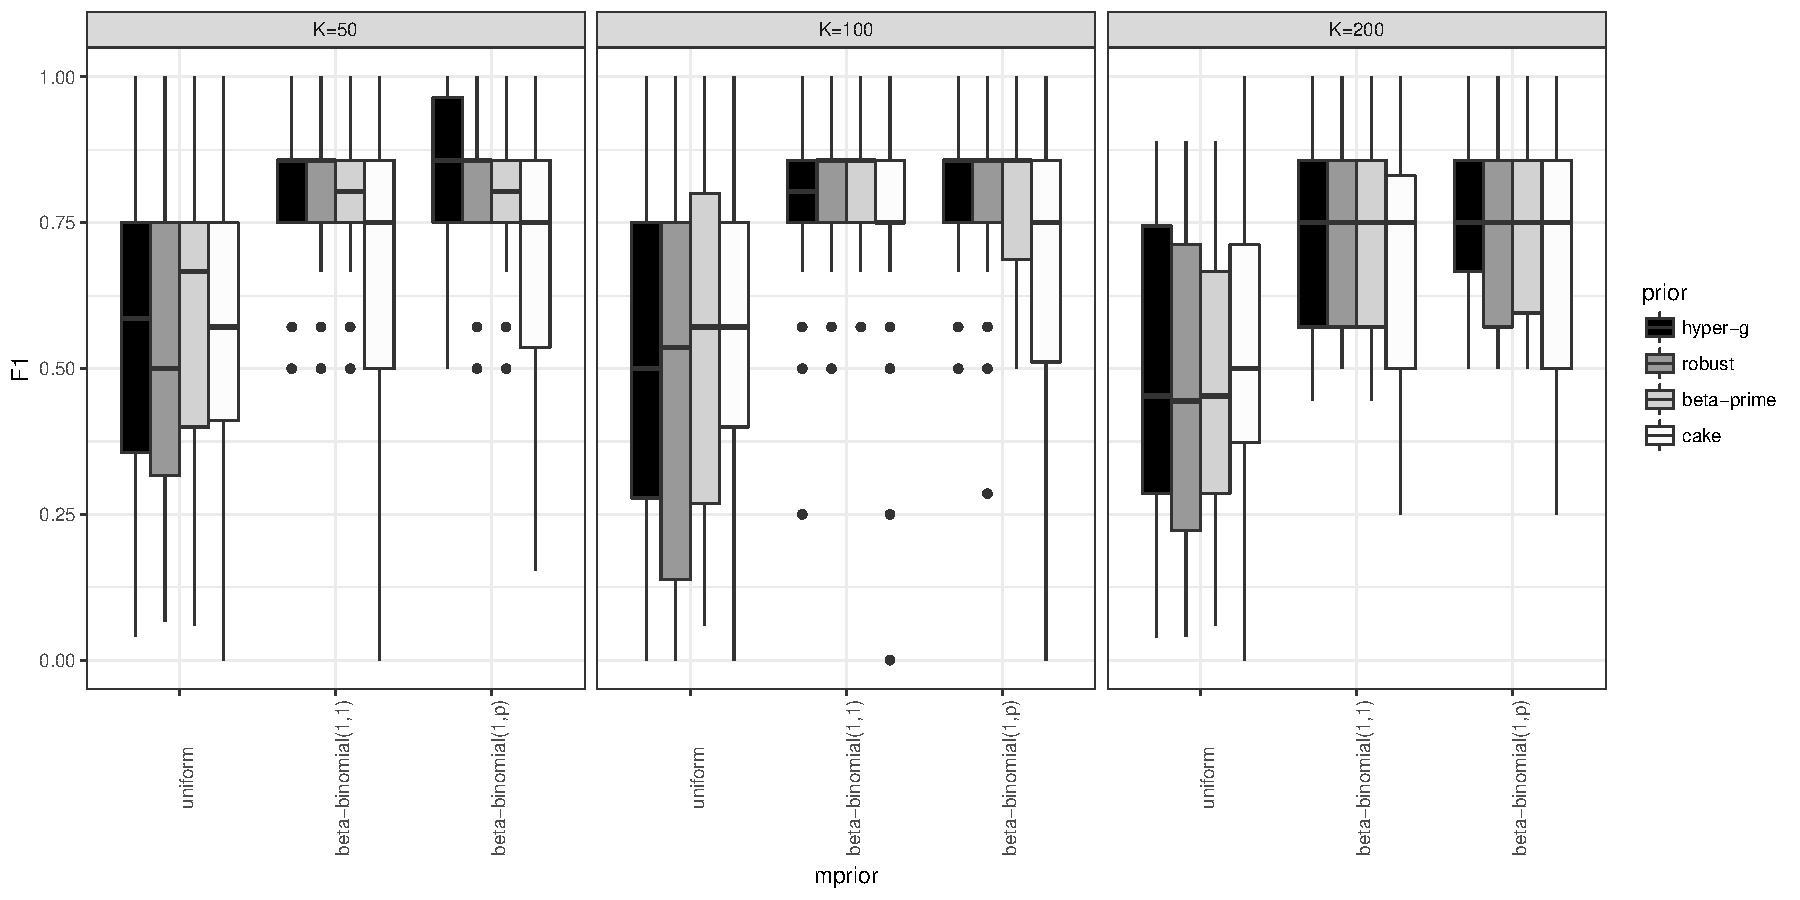
\includegraphics[width=0.95\textwidth]{./highDimPVA_F1.pdf}  
	\end{center}
	\caption{Comparison of the performance of the PVA method on the
						high-dimensional data set with different $g$ and $\vgamma$ priors using $F_1$ score.
						The hyper-$g$,
						robust Bayarri, Beta-prime and Cake priors on $g$ and the uniform, beta-binomial(1, 1) and beta-binomial(1, p) priors on $\vgamma$ are used.}
	\label{fig:highDimPVA_F1}
\end{figure}

\begin{figure}[h!]
	\begin{center}	
		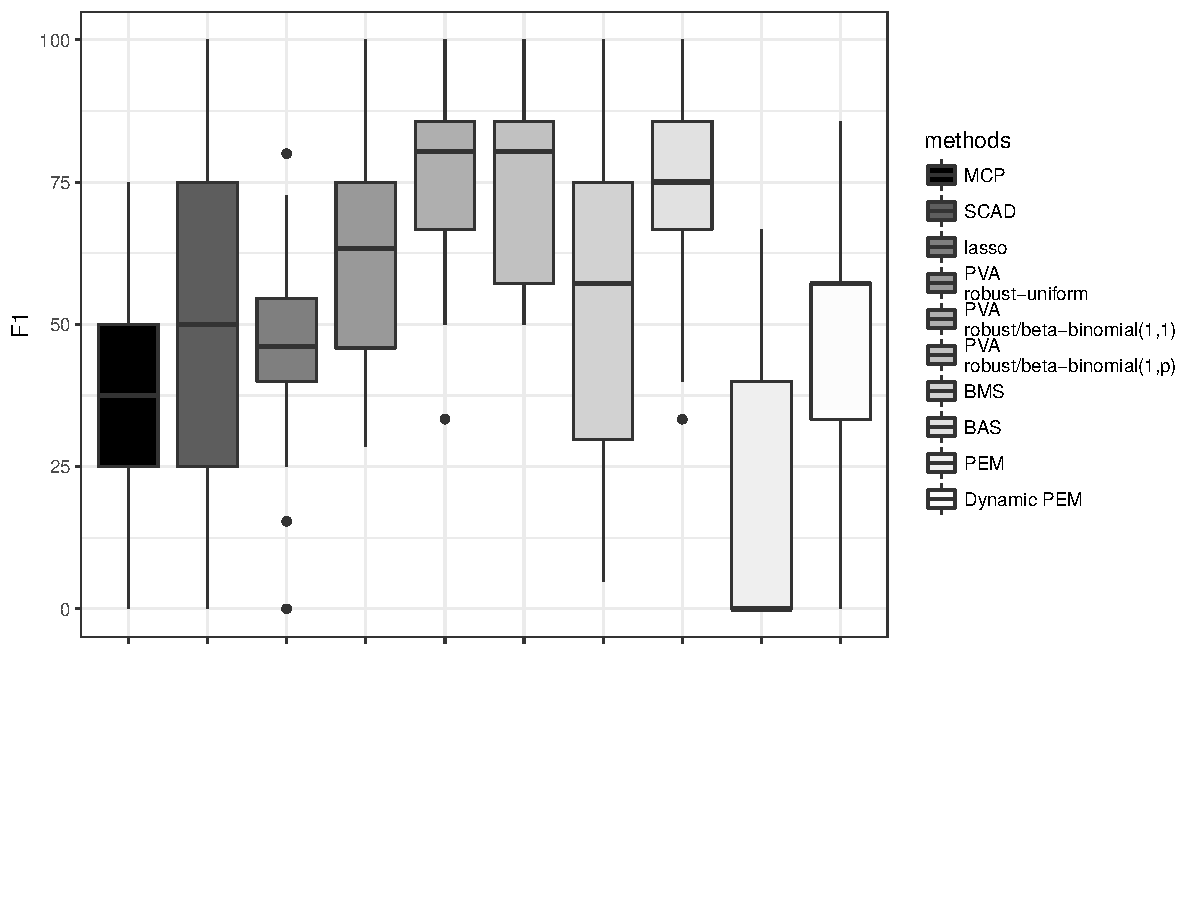
\includegraphics[trim={0 4cm 0 0},width=0.95\textwidth]{./highDimPVA_F1_compare_edit.pdf}  
	\end{center}
	\caption{Comparison of the performance of the MCP, SCAD, lasso, PVA, BMS, BAS and PEM methods on the
						high-dimensional data set using $F_1$ score. For PVA, the
						robust Bayarri prior on $g$ and the uniform, beta-binomial(1, 1) and beta-binomial(1, p) priors
						on $\vgamma$ are used.}
	\label{fig:highDimPVA_F1_compare}
\end{figure}

\subsubsection{Exploration of the posterior model space}

If the covariates in a model selection problem are highly collinear then the posterior distribution will be
highly multi-modal when a spike-and-slab prior structure is used. This can make seeking the optimal model very
challenging, due to the many local optima. In this section, we present a series of numerical experiments which
demonstrate the capability of our algorithm to successfully find the models with high posterior probability in
such situations.

Our population of bit strings $\mGamma^{(0)} = (\vgamma_1^{(0)}, \ldots, \vgamma_K^{(0)})$ with
$K = 20$ particles was randomly initialised from a sequence of independent Bernoulli trials with probability
of success $1/2$.
Figure \ref{fig:PVA_posterior_models} shows all $4096$ posterior model probabilities ordered by the model's
bit strings, represented by blue dots. Superimposed over this are the models found by PVA, represented by
red dots.
We can clearly see a few peaks in the full posterior distribution. Our experiment aims to show
that most of these posterior peaks are successfully identified by our algorithm.

As Figure \ref{fig:PVA_posterior_models} shows, 
in the plots of the log posterior probabilities of the models, the particles can be seen clustering at the
highest probability models first, then spreading through the medium and low probability models. From these
plots we can see that once $K$ is high enough, there is a good variety of high, medium and low posterior
probability models in the population of particles. The coverage of the posterior probability distribution
by the population of particles is high, as the particles tend to cluster towards the higher posterior
probability models as PVA's greedy search algorithm proceeds.

% We begin by using the setting $\lambda = 1$, allowing particle repulsion between each of the models within the
% population.

\begin{figure}	
	\includegraphics[width=0.95 \textwidth]{code/blma/cva_low_dimensional.pdf}
	\caption{Posterior model probabilities when $p = 12$. Red points denote models visited by the PVA
						algorithm, while blue points are models that were not visited. Note that the PVA algorithm
						visits the highest posterior probability points first}
	\label{fig:PVA_posterior_models}
\end{figure}

\subsection{Communities and crime dataset}
\label{sec:crime}

We use the {\tt Communities and Crime} dataset obtained from the
UCI Machine Learning Repository   \\

\url{http://archive.ics.uci.edu/ml/datasets/Communities+and+Crime}  \\

\noindent 
The data collected was part
of a study by \cite{Redmond2002} combining socio-economic data
from the 1990 United States Census, law enforcement data from the 1990 United States Law Enforcement Management and Administrative
Statistics
survey, and crime data from the 1995 Federal Bureau of Investigation's Uniform
Crime Reports.

The raw data consists of 2215 samples of 147 variables the first 5 of which
we regard as non-predictive, the next 124 are regarded as potential
covariates while the last 18 variables are regarded as potential response
variables. Roughly 15\% of the data is missing. We proceed with a complete
case analysis of the data.
We first remove any potential covariates which contained missing values leaving
101 covariates. We also remove the variables {\tt rentLowQ} and
{\tt medGrossRent} since these variables appeared to be nearly linear
combinations of the remaining variables (the matrix $\mX$ had two singular
values approximately $10^{-9}$ when these variables were included).  We use the
{\tt nonViolPerPop} variable as the response. We then remove any remaining
samples where the response is missing. The remaining dataset consist of 2118
samples and 99 covariates. Finally, the response and covariates are standardized to have mean 0 and standard deviation 1. Empirical correlations between variables range from $3.3\times10^{-5}$ to $0.999$.

A comparison of the performance of PVA for the hyper-$g$, robust Bayarri, Beta-prime and Cake priors on $g$
and the uniform, beta-binomial(1, 1) and beta-binomial(1, p) priors on $\vgamma$ using $F_1$ score is
presented in Figure \ref{fig:commPVA_F1}. A comparison of the performance of the MCP, SCAD, lasso, PVA, BMS,
BAS and PEM  methods using $F_1$ score is given in Figure \ref{fig:commPVA_F1_compare}.

\begin{figure}
	\begin{center}	
		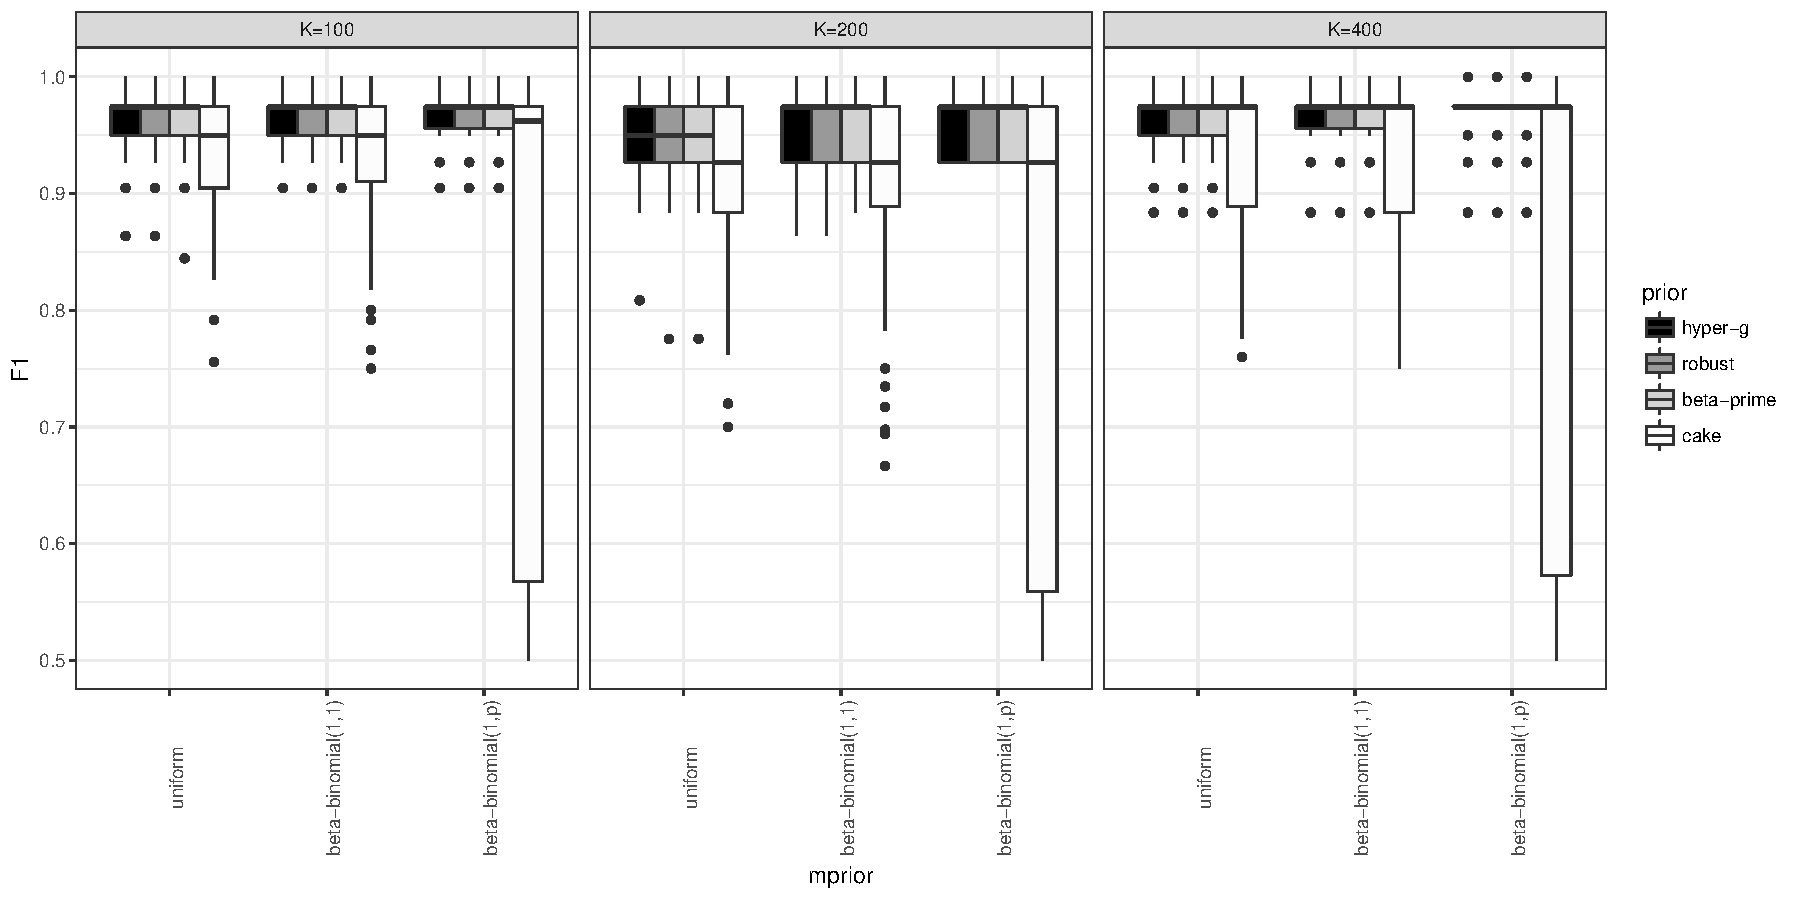
\includegraphics[width=0.95\textwidth]{./commPVA_F1.pdf}  
	\end{center}
	\caption{Comparison of the performance of the PVA method on the
						Communities and Crime data set with different $g$ and $\vgamma$ priors using $F_1$ score.
						The hyper-$g$,
						robust Bayarri, Beta-prime and Cake priors on $g$ and the uniform, beta-binomial(1, 1) and beta-binomial(1, p) priors on $\vgamma$ are used.}
	\label{fig:commPVA_F1}
\end{figure}

\begin{figure}
	\begin{center}	
		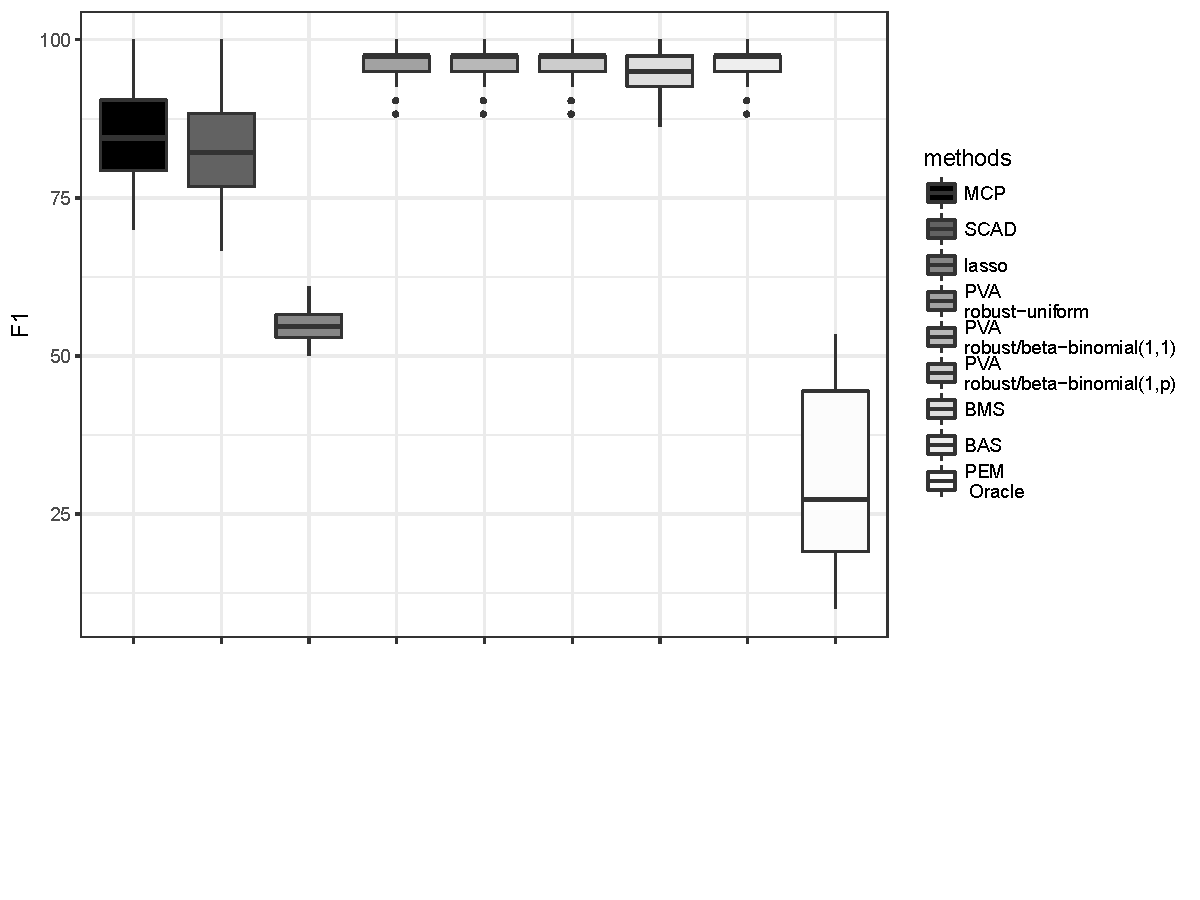
\includegraphics[trim={0 4cm 0 0},width=0.95\textwidth]{./commPVA_F1_compare_edit.pdf}  
	\end{center}
	\caption{Comparison of the performance of the MCP, SCAD, lasso, PVA, BMS, BAS and PEM methods on the
						Communities and Crime data set using $F_1$ score. For PVA, the
						robust Bayarri prior on $g$ and the uniform, beta-binomial(1, 1) and beta-binomial(1, p) priors
						on $\vgamma$ are used.}
	\label{fig:commPVA_F1_compare}
\end{figure}

\subsection{Quantitative trait loci dataset}
\label{sec:QTL}

	For our final $p>n$ simulation example we will use the design matrix based on an
experiment on a backcross population of $n=600$ individuals for a single large 
chromosome of 1800 cM. This giant chromosome was covered by 121 evenly 
spaced markers from \cite{Xu2007}. Nine of the markers overlapped with QTL ofthe main effects 
and 13 out of the ${121 \choose 2} = 7260$ possible marker pairs had interaction 
effects. The $\mX$ matrix combines the main effects and interaction effects to
make a $600\times 7381$ matrix. The values of the true coefficients are listed in 
Table 1 of \cite{Xu2007} ranging from 0.77 to 4.77 in absolute magnitude and
correlations range from 0 to 0.8 where most of the higher correlation occurs
along the off-diagonal values of the correlation matrix of the covariates. Here
we center the $\mX$ matrix and simulate new data from $\vy = \mX\vbeta_0 + \vvarepsilon$
where $\vvarepsilon = (\varepsilon_1,\ldots,\varepsilon_n)^\top$ and the $\vvarepsilon_i$
are independently drawn with $\vvarepsilon_i \sim N(0,20)$. Similar simulation
studies were conducted in \cite{Xu2007} and \cite{Karkkainen2012}. This
process was repeated $50$ times.
For this simulation setting PVA has the best model selection accuracy,
smallest MSEs and smallest parameter biases of all the methods compared.
The Lasso, SCAD, MCP, EMVS, PVA and BMS methods took 1.5, 1.5, 1.8, 1229, 2011, 5327
seconds respectively.

A comparison of the performance of PVA for the hyper-$g$, robust Bayarri, Beta-prime and Cake priors on $g$
and the uniform, $\text{beta-binomial}(1, 1)$ and $\text{beta-binomial}(1, p)$ priors on $\vgamma$ using $F_1$
score is presented in Figure \ref{fig:qtlPVA_F1}. A comparison of the performance of the MCP, SCAD, lasso,
PVA, BMS, BAS and PEM  methods using $F_1$ score is given in Figure \ref{fig:qtlPVA_F1_compare}.

\begin{figure}[h!]
	\begin{center}	
		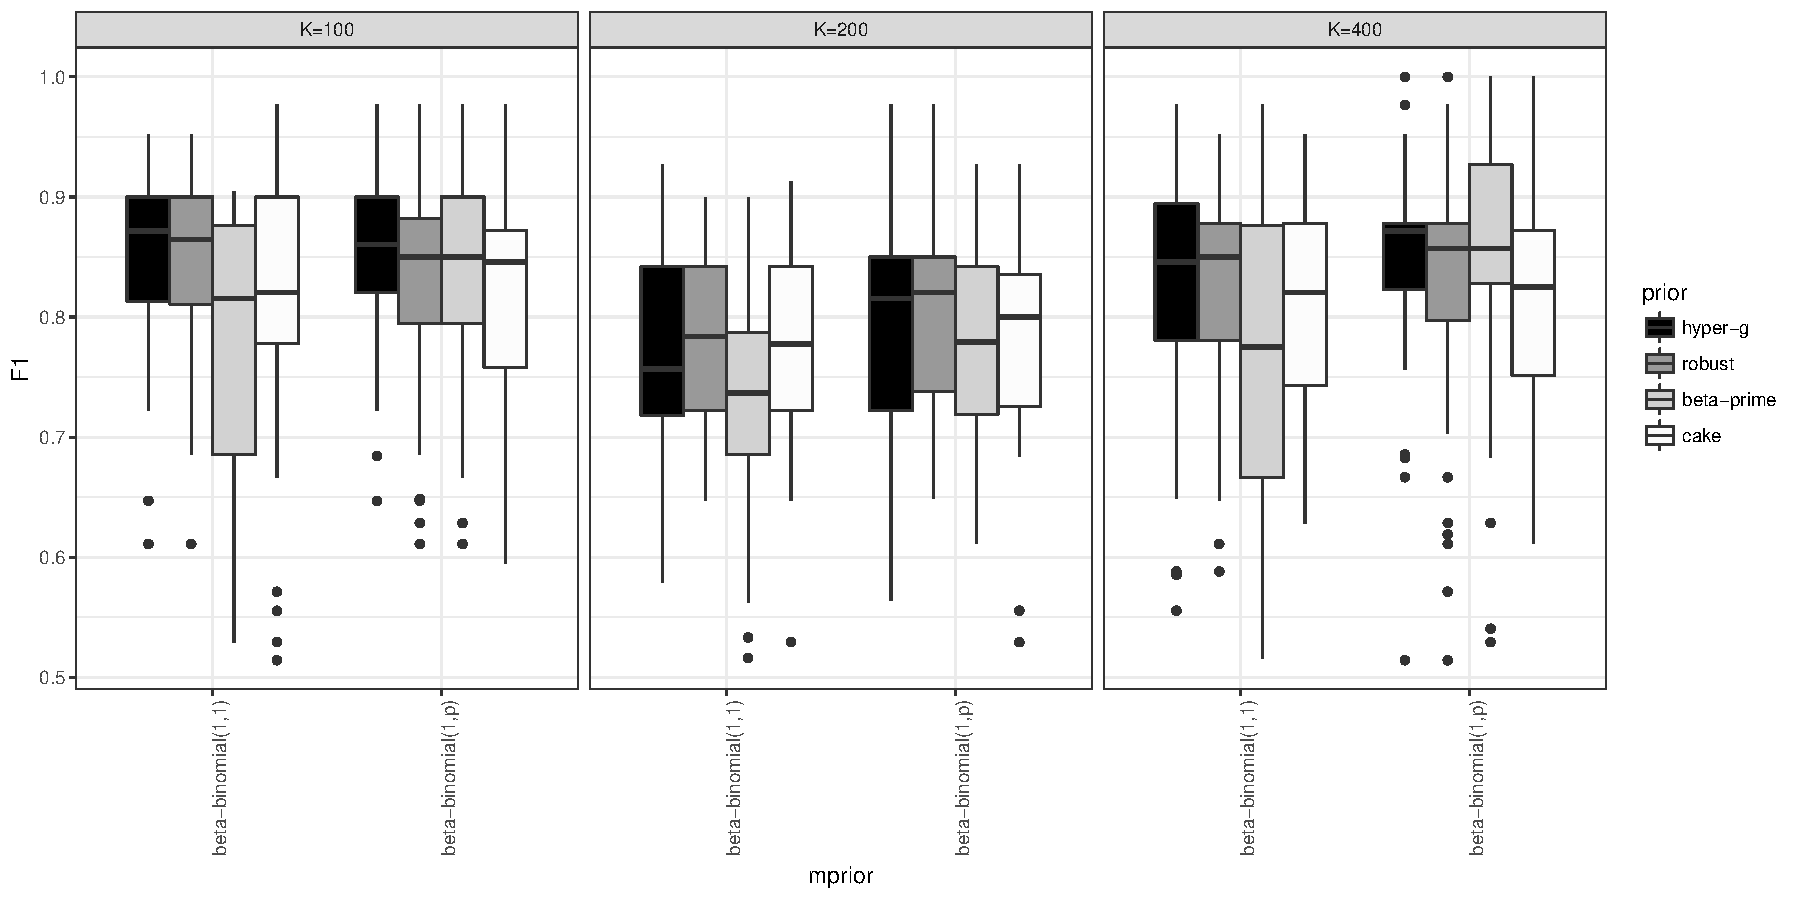
\includegraphics[width=0.95\textwidth]{./qtlPVA_F1.pdf}  
	\end{center}
	\caption{Comparison of the performance of the PVA method on the
						QTL data set with different $g$ and $\vgamma$ priors using $F_1$ score.
						The hyper-$g$,
						robust Bayarri, Beta-prime and Cake priors on $g$ and the uniform, beta-binomial(1, 1) and beta-binomial(1, p) priors on $\vgamma$ are used.}
	\label{fig:qtlPVA_F1}
\end{figure}

\begin{figure}[h!]
	\begin{center}	
		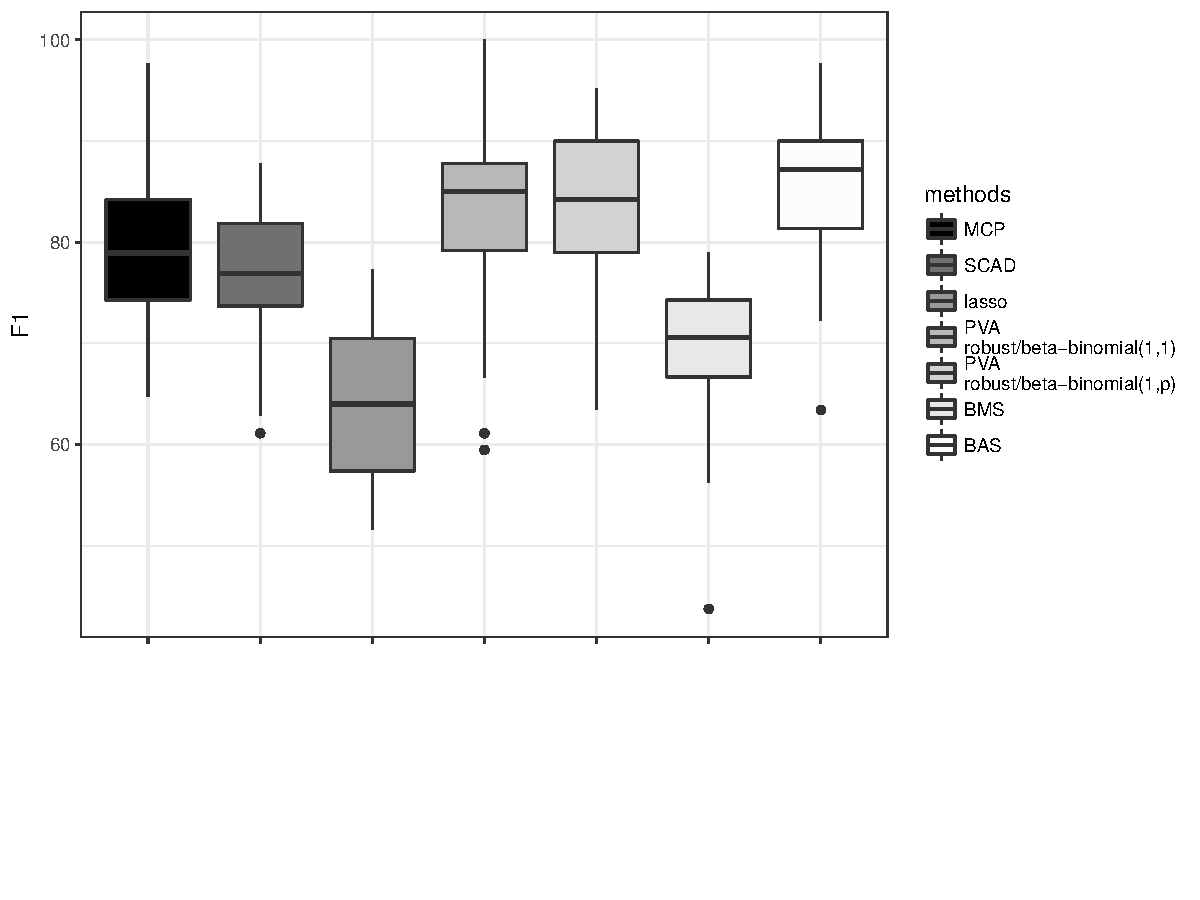
\includegraphics[trim={0 4cm 0 0},width=0.95\textwidth]{./qtlPVA_F1_compare_edit.pdf}  
	\end{center}
	\caption{Comparison of the performance of the MCP, SCAD, lasso, PVA, BMS, BAS and PEM methods on the
						QTL data set using $F_1$ score. For PVA, the
						robust Bayarri prior on $g$ and the uniform, beta-binomial(1, 1) and beta-binomial(1, p) priors
						on $\vgamma$ are used.}
	\label{fig:qtlPVA_F1_compare}
\end{figure}


% Mine
% \subsection{$n < p$, High dimensional example, Particle EM}

% We first present an example where $n > p$ and $p$ is relatively small ($p = 12$), to allow for the full
% enumeration of the model space. Later, we show an example for the important $p > n$ case. We compare our
% results  against the Lasso (\cite{Tibshirani1996}), SCAD (\cite{Fan2001}), MCP (\cite{Zhang2010}), {\tt BMS}
% (\cite{Zeugner2015}) and {\tt VARBVS} (\cite{Carbonetto2012}) algorithms.


% \subsection{$p > n$}

% \begin{table}
% 	\caption{Simulation results including the average number of modes located, the average percentage of
% 	posterior coverage achieved, and the percentage of times that the global mode was located, for various
% 	population sizes $(K=20, 50, 100)$ and choices of repulsion $\lambda=0, 1, 2, 3$}
% 	\label{tab:result2}
% 	\begin{tabular}{l|llll|llll|llll|llll}
% 	\hline
% 	 					& \multicolumn{4}{c}{K=20} 	& \multicolumn{4}{c}{K=50} & \multicolumn{4}{c}{K=100} \\
% 	$\lambda$ & 0 & 1 & 2 & 3 & 0 & 1 & 2 & 3 & 0 & 1 & 2 & 3 & 0 & 1 & 2 & 3 \\
% 	\hline
% 	\# Modes & \\
% 	\% Posterior & 83.1 & 84.7 & 83.7 & 82.3 & 84.7 & 83.2 & 85.4 & 84.8 & 81.9 & 82.9 & 83.9 & 84.6 & 83.9 & 81.5 & 82.0 & 85.2 \\
% 	\% Global Mode & 91 & 90 & 87 & 82 & 86 & 85 & 80 & 90 & 90 & 90 & 86 & 91 & 88 & 91 & 76 & 88 \\
% 	\hline
% 	\end{tabular}

% \end{table}

% Show posterior probabilities on the log scale

\subsection{Comparison of PVA against other model selection methods on simulated data sets}

	% TP <- sum(vgamma.hat[pos])
	% TN <- sum(1 - vgamma.hat[neg])
	% FP <- sum(vgamma.hat[neg])
	% FN <- sum(1 - vgamma.hat[pos])
	
	% sensitivity <- TP/length(pos)
	% specificity <- TN/length(neg)
	% precision <- TP/sum(vgamma.hat)
	% recall <- TP/(TP + FN)
	% accuracy <- (TP + TN)/(TP + TN + FP + FN)
		
	% F1 <- 2*precision*recall/(precision+recall)		

The method used to assess the quality of the variable selection was to generate data from a known true model
$\vgamma$, and then compare this against the model $\widehat{\vgamma}$ found by each of the model selection
methods that we  compared. We then calculated the $F_1$ score for $\widehat{\vgamma}$.

% ,

% where
% $$F_1 = 2 \times \text{precision} \times \text{recall} / (\text{precision} + \text{recall})$$ with
% $\text{precision} = \text{true positives} / (\text{true positives} + \text{false positives})$ and
% $\text{recall} = \text{true positives} / (\text{true positives} + \text{false negatives})$.

% When running PVA,
% three methods of initialising $\Gamma$ were tried.
% A cold start where each $\gamma_{ij}$ in $\gamma_i$, $1 \leq i \leq K$ was initialised randomly from a
% $\text{Bernoulli}(p)$ distribution, with $p = 10 / |\vgamma|$.

% Two methods of warm start were also tried, to explore whether the PVA algorithm could do better by being
% initialised from another method than by being initialised randomly: 
% a warm start from SCAD where models with more covariates were preferred, and
% a warm start from SCAD where models with higher likelihood were preferred.

The experiments were repeated with 
the Cake prior, Maruyama's Beta-prime prior, Liang's hyper-g prior and Bayarri's robust prior.
The results of the algorithm were found to be insensitive to the choice of prior.
For each combination of population size, data set, and prior the experiment was repeated 50 times.

% \subsubsection{High-dimensional example $p > n$, Quantitative Trait Locus}
% The Quantitative Trait Locus (QTL) example is taken from \cite{Xu2007}. A BC population of $n=600$ was
% simulated for a single large chromosome of $1800$ cM. This chromosome was covered by 121 evenly spaced
% markers. Nine of the markers overlapped with QTL of the main effects and 13 out of the $\binom{121} 2 = 7,260$
% possible marker pairs had interaction effects.

% The PVA method was compared against Lasso, SCAD, Mcp, BMS and VARBVS. The {\tt BMS} method was run with
% $1,000,000$ iterations. While the $F_1$ scores from this method were excellent, the runtimes of the BMS method
% with this number of iterations were prohibively long - from 10 minutes to half an hour. When the number of
% iterations was reduced to $100,000$ less, the resulting $F_1$ scores were much poorer. The {\tt VARBVS} method
% was run with $\sigma = 10.0$ and $sa = 10.0$, which improved the $F_1$ score obtained.

% When initialising $\Gamma$ with a warm start from SCAD preferring models with more covariates or with higher
% likelihood, PVA performed poorly with a lower number of particles (K=$20$). Performance improved as the number
% of particles in the population was increased, as can be seen in Figures \ref{fig:QTL_warm_start_covariates}
% and \ref{fig:QTL_warm_start_likelihood}. Performance was better when $\Gamma$ was initialised randomly, for
% all population sizes $K=20$, $50$ or $100$.  PVA consistently achieved $F_1$ scores that were either
% competitive with or higher than the competing methods that we examined. This indicates that the PVA algorithm
% is sensitive to its' initialisation, and that as SCAD does poorly on these problems, PVA also does poorly
% comparatively with a warm start from SCAD, although still better than SCAD alone.

% \begin{figure}
% \includegraphics[width=0.95 \textwidth]{QTL_covariates_maruyama.pdf}
% \label{fig:QTL_warm_start_covariates}
% \caption{$F_1$ scores for PVA on the simulated QTL data with $\Gamma$ initialised from the SCAD models, with
% models with more covariates preferred. Here $K=20$, $50$ and $100$ respectively}
% \includegraphics[scale=0.33]{code/QTL/results/20_generate_data_QTL_warm_start_covariates_log_prob1.pdf}
% \includegraphics[scale=0.33]{code/QTL/results/50_generate_data_QTL_warm_start_covariates_log_prob1.pdf}
% \includegraphics[scale=0.33]{code/QTL/results/100_generate_data_QTL_warm_start_covariates_log_prob1.pdf}
% \end{figure}

% \begin{figure}
% \includegraphics[width=0.95 \textwidth]{QTL_likelihood_maruyama.pdf}
% \label{fig:QTL_warm_start_likelihood}
% \caption{$F_1$ scores for PVA on the simulated QTL data with $\Gamma$ initialised from the SCAD models, with
% models with higher likelihood preferred. Here $K=20$, $50$ and $100$ respectively}
% \end{figure}


% Initialising $\Gamma$ randomly, PVA performed poorly by comparison with either of the warm start methods
% above, as can be seen from Figure \ref{fig:QTL_cold_start}.
% \begin{figure}
% \includegraphics[width=0.95 \textwidth]{QTL_cold_maruyama.pdf}
% \label{fig:QTL_cold_start}
% \caption{$F_1$ scores for PVA on the simulated QTL data with $\Gamma$ initialised randomly.
% 					Here $K=20$, $50$ and $100$ respectively}
% \includegraphics[scale=0.33]{code/QTL/results/20_generate_data_QTL_cold_start_log_prob1.pdf}
% \includegraphics[scale=0.33]{code/QTL/results/50_generate_data_QTL_cold_start_log_prob1.pdf}
% \includegraphics[scale=0.33]{code/QTL/results/100_generate_data_QTL_cold_start_log_prob1.pdf}
% \end{figure}

% When initialising $\Gamma$ with a warm start from SCAD preferring models with higher likelihood,
% PVA performed less well on the QTL example than SCAD preferring models with more covariates, but still
% better than other competing methods except for MCP,
% as can be seen from Figure \ref{fig:QTL_warm_start_likelihood}

\section{Variable inclusion for small data sets}

We compared variable selection using PVA against exact variable selection on five small data sets,
Hitters, Bodyfat, Wage, College and US Crime. 
The variable inclusion probabilities were estimated by taking the sum of the columns of the population
of models selected $\mGamma$
weighted by marginal likelihood of each model.
The exact variable inclusion probabilities were calculated by summing the columns of the matrix of all possible
models $\mGamma$ weighted by the marginal likelihood of each model.
The mean relative error of the variable inclusion probabilities estimated by PVA was calculated,
and the results of these comparisons are presented in Table \ref{tab:variable_inclusion_rel_error}.
The number of particles in the population $K$ affected the
variable inclusion probability in the variables selected by PVA, while the marginal probability
$p(\vgamma | \vy)$ used to weight models in $\Gamma$ seemed to have only a very minor impact.
% Is this still true?
When the robust Bayarri prior is chosen to rank models in PVA,
the marginal probability $p(\vgamma | \vy)$ changes a lot as opposed to ranking models with other priors.
From the previous section, we see that changing the PVA model ranking
marginal had a large impact on the $F_1$ score obtained.
Variables with low posterior probability are truncated to 0, as PVA seeks higher posterior probability models,
ignoring the lower posterior probability models.

\begin{table}[!ht]
\begin{tabular}{|ll|rrr|rrr|}
	\hline
	Dataset & Prior & & $<=0.5$ & & & $>0.5$ &\\
	& & $K = 20$ & $K = 50$ & $K = 100$ & $K = 20$ & $K = 50$ & $K = 100$ \\
	\hline
	Bodyfat&BIC&$0.63$&$0.48$&$0.37$&$0.07$&$0.01$&$0.02$\\
	&Liang's hyper-$g$ prior&$0.66$&$0.52$&$0.42$&$0.07$&$0.01$&$0.02$\\
	&Bayarri's robust prior&$0.65$&$0.52$&$0.4$&$0.07$&$0.01$&$0.02$\\
	&ZE&$0.65$&$0.51$&$0.39$&$0.06$&$0.01$&$0.02$\\
	College&BIC&$0.7$&$0.58$&$0.49$&$0.03$&$0.02$&$0.03$\\
	&Liang's hyper-$g$ prior&$0.9$&$0.78$&$0.64$&$0.06$&$0.06$&$0.06$\\
	&Bayarri's robust prior&$0.88$&$0.78$&$0.63$&$0.06$&$0.06$&$0.06$\\
	&ZE&$0.82$&$0.66$&$0.57$&$0.03$&$0.06$&$0.06$\\
	Hitters&BIC&$0.74$&$0.64$&$0.5$&$0.12$&$0.07$&$0.06$\\
	&Liang's hyper-$g$ prior&NA&$0.81$&$0.83$&NA&$0.17$&$0.07$\\
	&Bayarri's robust prior&$0.84$&$0.81$&$0.75$&$0.29$&$0.17$&$0.07$\\
	&ZE&$0.79$&$0.72$&$0.67$&$0.27$&$0.13$&$0.05$\\
	USCrime&BIC&$0.82$&$0.7$&$0.64$&$0.47$&$0.15$&$0.12$\\
	&Liang's hyper-$g$ prior&$0.76$&$0.71$&$0.64$&$0.45$&$0.16$&$0.12$\\
	&Bayarri's robust prior&$0.79$&$0.7$&$0.61$&$0.35$&$0.14$&$0.08$\\
	&ZE&$0.76$&$0.7$&$0.64$&$0.45$&$0.16$&$0.13$\\
	Wage&BIC&$0.67$&$0.49$&$0.35$&$0$&$0$&$0$\\
	&Liang's hyper-$g$ prior&$0.69$&$0.47$&$0.33$&$0$&$0$&$0$\\
	&Bayarri's robust prior&$0.69$&$0.47$&$0.32$&$0$&$0$&$0$\\
	&ZE&$0.69$&$0.47$&$0.32$&$0$&$0$&$0$\\
	\hline
\end{tabular}
\label{tab:variable_inclusion_rel_error}
\caption{Relative error of the variable inclusion probability estimated by PVA to the
					exact variable inclusion probability, partitioned by exact probability under or equal to $0.5$ and
					over $0.5$}
\end{table}

% Small data set, Kakadu
\begin{figure}[ht!]
	\includegraphics[scale=0.5]{posterior_prob_Kakadu.pdf}
	\includegraphics[scale=0.5]{inclusion_error_Kakadu.pdf}

	\caption{PVA was run on the Kakadu data set. The total posterior model probability and error in posterior 
						variable inclusion probability were calculated using the exact posterior model and variable  
						inclusion probability from every possible sub-model. These were calculated for a range of 
						population sizes from 25 to 500, in 25 model increments.
						As the population increases, the total posterior model probability increases while the error in 
						posterior variable inclusion probabliity decreases.}
	\label{fig:kakadu_total_posterior_mass}
\end{figure}

% VietNam
% GradRate
% UScrime

% Interpretation of results
The same general trends were observed in all small data sets. Total posterior probability is higher for the
beta- binomial model prior than for the uniform model prior, while the variable inclusion error is lower. This
same general trend is seen regardless of $g$-prior. Total posterior probability increases with increased
population size $K$, while variable inclusion error decreases. Although the PVA algorithm is deterministic,
variation in the results amongst the trials is seen due to the random initialisation of $\mGamma$.

\section{Conclusion}
\label{sec:chapter_4_conclusion}
We have proposed a deterministic Bayesian model selection algorithm which is computationally efficient
and simple. Like Particle EM \cite{Rockova2017}, our algorithm maintains a population of solutions and ensures
diversity of that population to explore the uncertainty of the selected model. This gives far more information
about the model selection process than simply choosing one best model. However, whereas Particle EM uses
a spike-and-slab prior for the regression co-efficients, our approach uses a g-prior, which avoids 
the Bartlett's Paradox and Information Paradox. Importantly, both approaches can be implemented using rank-one
updates and downdates and the model selection posterior probabilities are available in closed form,
which allows the algorithm to be implemented in a computionally efficient manner.

While previously model selection algorithms using the Maruyama, Liang-g and robust Bayarri priors have
typically been implemented using Monte Carlo Markov Chains, our algorithm allows the advantages of these
priors while using a deterministic algorithm. The PVA algorithm  presented in this chapter is implemented in
the {\tt blma} package in the {\tt cva} function.

\chapter{Conclusion}

\section{Zero-inflated models Discussion}
\label{sec:discussion}
		
We have described a Variational Bayes approximation to Zero-Inflated Poisson regression models which
allows such models to be fit with considerable generality. We have also devised and extensively tested a
number of alternative approaches for fitting such models, and extended one of these alternative
approaches with a new parameterisation. Using MCMC methods as the gold standard to test against, we have
assessed the accuracy and computational speed of these algoritms.
		
We applied our model fitting algorithms to a number of data sets to fit a range of models. The Cockroaches
model \ref{sec:cockroaches} had few fixed covariates, a random intercept for each apartment building and
incorporated zero-inflation. The Police stops model \ref{sec:police_stops} was a pure Poisson mixed model, no
zero-inflation and a random intercept for precincts/locality. The Biochemists model \ref{sec:biochemists} was
zero-inflated with fixed effects. The Owls model \ref{sec:owls} was zero-inflated, random intercepts for
nests. There were a large number of nests. We were able to estimate the variance component for this model very
accurately.

The use of Mean Field Variational Bayes allows estimation of Bayesian ZIP models in a fraction of the
time taken to fit the same model using even the best MCMC methods available, with only a small loss of
accuracy. This is of great utility in applications where speed matters, such as model selection or when
applied statisticians are choosing amongst many candidate models, as is typical in practice.
		
The new parameterisation of Gaussian Variational Approximation using the Cholesky factorisation of the
inverse of $\mLambda$ presented in Section \ref{sec:param} provides significant advantages.  It is well
known that the inverse of a sparse matrix need not be sparse.

Mixed models have covariance matrices with a block structure, due to the dependence structure of the
random effects. The precision parameterisation presented in this chapter is able to preserve this
sparsity within the structure of the Cholesky factors of the inverses of the covariance matrices use in
the variational lower bound by re-ordering the rows and columns of the matrices so that the random
effects blocks appear first. The Owls example presented in this chapter shows the computational
advantages of this approach when the number of groups $m$ in the model is large (m=27 in this case) --
as the covariance parameterisation takes 46 seconds to fit whereas the inverse parameterisation only
takes 3 seconds. This clearly demonstrates advantage of using sparsity to reduce the dimension of the
optimisation problem to be solved when models are being fit -- as only the non-zero values in the
covariance matrices need to be optimised over. This allows models to be fit more quickly, and with
greatly improved numerical stability and without loss of accuracy.

While all of the fitting algorithms presented in this chapter except the Laplace's approximation
algorithm were able to fit ZIP random and fixed effects models with high accuracy, and the 
Gaussian inverse parameterisation and fixed point algorithms were able to do so at high speed, they 
could be numerically unstable depending on the data the model was being fit to and their starting points.
In the case of the Gaussian inverse parameterisation algorithm, the source of the problem was tracked down
to the exponential used in the parameterisation of the diagonal of the Cholesky factor of the precision
matrix combined with the exponential that arises in the derivation of the Gaussian variational lower
bound for Poisson mixed models -- leading to frequent numeric overflows during the fitting process. This
problem, once discovered, was mitigated by replacing the exponential parameterisation of the diagonal
of the Cholesky factor with a piecewise function which is exponential beneath a threshold and quadratic
above that threshold. This was shown to greatly increase the numeric stability of the GVA inverse
parameterisation for a range of starting points.

Some of the algorithms which we experimented with were found to be very sensitive to their starting points.
While these algorithms are typically initialised with a starting point as close as possible to the final
solution, this gives some sense of the stability of each algorithm.
Stability fixes.

This article presents the essential ideas necessary for a performant implementation implementing model fitting
for ZIP regression models.%, but the performance would be even better if our algorithm was re-implemented in a
%compiled language with good numeric libraries such as C++ with Eigen.
The majority of the performance
improvements over existing approaches come from avoiding unneccessary matrix inversion, which is a
computationally expensive and numerically unstable process taking $\BigO(p^3)$ flops, and from constructing and 
calculating	with sparse matrices. The gains of these approaches, particularly from sparse matrix techniques, 
can be difficult to fully realise in R without expert knowledge of the underlying implementation and libraries.
		
Our application of these ideas to Andrew Gelman's data showed that the new parameterisation very effectively
speeds up fitting zero-inflated mixed models to real world data with a large number of groups, while still
maintaining excellent accuracy versus an MCMC approach. This demonstrates the applicability of the ideas
presented within this paper to real world data sets.
		
\section{CVA Conclusion}

We have proposed a deterministic Bayesian model selection algorithm which is computationally efficient
and simple. Like Particle EM \cite{Rockova2017}, our algorithm maintains a population of solutions and ensures
diversity of that population to explore the uncertainty of the selected model. This gives far more information
about the model selection process than simply choosing one best model. However, whereas Particle EM uses
a spike-and-slab prior for the regression co-efficients, our approach uses a g-prior, which avoids 
the Bartlett's Paradox and Information Paradox. Importantly, both approaches can be implemented using rank-one
updates and downdates and the model selection posterior probabilities are available in closed form.

While previously model selection algorithms using the Maruyama, Liang-g and robust Bayarri priors have
typically been implemented using Monte Carlo Markov Chains, our algorithm allows the advantages of these
priors while using a deterministic algorithm.

The CVA algorithm is implemented in the {\tt blma} package in the {\tt cva} function.

% \chapter{Posterior distributions of regression model parameters under Maruyama's Beta-Prime prior}

\section{Introduction}

In this chapter, we consider
a linear model with $g$-priors used for model selection, as in \citep{Maruyama2011}. 
In most cases, we derive exact expressions for the posterior distributions of the regression parameters of
this model. Where this is analytically intractable, we derive exact expressions for the expectation and
covariance of the regression parameters, and develop a Laplace approximation to the posterior distribution
of the regression parameters.

% Structured Variational Bayes for model selection, Wand and Ormerod Variational Bayes for Elaborate 
% Distributions (\citep{Wand2011})

% Application

% VB theory

% Our main contribution
In this paper, we develop Variational Bayes approximations to model selection of linear models using Zellner's
g prior as in \citep{Liang2008}.

% By searching of the model space as one covariate changes between each sub-model and  using rank-1 updates on
% $(\mX^\top \mX)^{-1}$, we are able to exhaustively search the model space in $\BigO(2^p np^2)$ rather than
% $\BigO(2^p np^3)$.

% This article is organised as follows. In Section \ref{sec:model_selection}, we review previous Bayesian
% approaches to model selection. 
In Section \ref{sec:methodology} we develop our approach. In Section
\ref{sec:num_exp} we perform a series of numerical experiments to show the accuracy of our approach. Finally,
in Section \ref{sec:conclusion}, we provide a Conclusion and Discussion.

\section{Methodology}
\label{sec:methodology}

\subsection{Notation}

% Definitions

Let $n > 0$ be the number of observations and $p > 0$ be the number of covariates. Let $\vy \in \R^n$ be the
vector of responses, $\vtheta \in \R^p$ be the vector of parameters and $\mX \in \R^{n \times p}$ be the
matrix of covariates. Let $p(\vtheta)$ be the prior distribution of $\vtheta$, $p(\vy, \vtheta)$ be the full
probability distribution of $\vy$, $p(\vtheta | \vy)$ the posterior distribution and $q(\vtheta)$ be the
approximating probability distribution. 

\subsection{Model}
\label{sec:model}

Zellner constructed the $g$-prior family of priors for a Gaussian regression model using a particular form of
conjugate Normal-Gamma model, where the prior covariance matrix of $\vbeta$ is taken to be a multiple of the
Fisher information  matrix by the parameter $g$ \citep{Zellner1986}. This could be thought of as regularisation
in the principle components of the estimated covariance matrix. This places the most prior mass for $\vbeta$
on the section of the parameter space where the data is least informative.

We consider a normal linear model on $\vy$ with conjugate normal prior on $\vbeta$, and covariance $g \sigma^2
(\mX^\top \mX)^{-1}$ where the prior on $g$ is Zellner's g-prior on the covariance matrices, 
We consider a normal linear model with a $g$-prior on the regression co-efficients $\vbeta$.
This introduces a hyperparameter $g$ which controls the shrinkage of the regressions co-efficients.
The prior on $g$ can be carefully chosen so that the other parameters in the model can be integrated out
analytically, yielding tractable marginal and posterior distributions for $g$, as shown by \citep{Liang2008}.
Several priors on $g$ have been considered in the literature, including the hyper-$g$ and hyper-$g/n$ priors
\cite{Liang2008}, Bayarri's robust prior \cite{Bayarri2012} and the Beta-Prime prior introduced by
\citep{Maruyama2011}. We choose the popular Beta-Prime prior, as it is numerically well-behaved. 
We choose $a$  and $b$ to be $-3/4$ and $(n - p)/2 - a - 2$ respectively, following \citep{Maruyama2011}.

\section{The base model}
\label{sec:model}

Suppose $\vy = (y_1,\ldots,y_n)^T$ is a response vector of length $n$, $\mX$ is an $n$ by $p$ matrix 
of covariates. We consider the linear model for predicting $\vy$ with predicturs $\mX$ via
\begin{equation}
\label{eq:linearModel}
\vy | \alpha, \vbeta, \sigma^2 \sim N(\vone_n\alpha + \mX \vbeta, \sigma^2 \mI_n),
\end{equation} 


\noindent where $\alpha$ is the model intercept, $\vbeta$ is a coefficient vector of length $p$, 
$\sigma^2$ is the residual variance, and $\mI_n$ is the $n \times n$ identity matrix. 
Without loss of generality, to simplify later calculations, we will transform $\vy$ and $\mX$ 
so that $\vy$ and the columns of $\mX$ are standardized so that $\overline{y} = 0$, 
$\|\vy\|^2 = \vy^T\vy = n$, $\mX_j^T\vone = 0$,  and $\|\mX_j\|^2 = n$ where $\mX_j$ is the $j$th  column of $\mX$. 

Suppose that we wish to perform Bayesian model selection, model averaging or hypothesis 
testing. Let $\vgamma \in \{0, 1\}^p$ be a binary vector of indicators
for the inclusion of the $p$th column of $\mX$ in the model where $\mX_\vgamma$ 
denotes the design matrix formed by including only the columns of $\mX$ with 
$\gamma_j = 1$. We will adopt the following prior structure
\begin{equation}
\label{eq:priorStructure}
\begin{array}{c}
\ds p(\alpha) \propto 1,  
\qquad 
\ds p(\sigma^2) \propto (\sigma^2)^{-1} I(\sigma^2 > 0),                      
\\ [2ex]
\vbeta_\vgamma | \sigma^2, g, \vgamma \sim \N_p(\vzero, g \sigma^2 (\mX_\vgamma^T \mX_\vgamma)^{-1}),
\quad \text{ and }  \quad 
p(\vbeta_{-\vgamma}|\vgamma) = \prod_{j=1}^p \delta(\beta_j;0)^{1-\gamma_j},
\end{array}
\end{equation} 

\noindent where $\delta(x;a)$ is the Dirac delta function with location $a$. 
For the time being we will defer specification of $p(g)$ and $p(\vgamma)$.
We will now justify each element of our chosen prior structure.

The priors on $\alpha$ and $\sigma^2$ are improper Jeffreys priors and have been formally justified 
in \cite{Berger2012}. In the context Bayesian model selection, model averaging or hypothesis 
testing $\alpha$ and $\sigma^2$ appear in all models 
so that when comparing models the proportionality constants in the corresponding
Bayes factors cancel.

The prior on $\vbeta_\vgamma$ is Zellner's $g$-prior \citep[see for example,][]{Zellner1986} with prior 
hyperparameter $g$. This family of priors for Gaussian regression model where the prior covariance 
matrix of $\vbeta_\vgamma$ is taken to be a multiple of $g$ with the Fisher information matrix for $\vbeta$. 
This places the most prior mass for $\vbeta_\vgamma$ on the section of the parameter space where the data is 
least informative, and makes the marginal likelihood of the model scale-invariant. Furthermore, this 
choice of prior removes a log-determinant of $\mX_\vgamma^T\mX_\vgamma$ term from the expression for the marginal 
likelihood, which is an additional computational burden to calculate.

\section{Exact posterior distributions in terms of special functions}
\label{sec:Exact}
 
In this section we derive the exact expressions for most Bayesian inferential quantities
of interest based on the model presented in Section 2. An exception is
the exact expression for the posterior density for $\vbeta|\vy$ for this quantity we
instead derive the first and second moments.


First, we use the fact that $p(\sigma^2|\vy) = \int_0^\infty p(\sigma^2|\vy,u) p(u|\vy)dg$ so that the density
$\sigma^2|\vy$ may be expressed as
$$
\begin{array}{rl}
\ds p(\sigma^2|\vy) 
%& \ds = 
%\left[ \frac{\left(\tfrac{n}{2}\right)^c}{\Gamma(c)} (\sigma^2)^{-(c+1)} \exp\left\{ - \frac{n}{2\sigma^2} \right\} \right] 
%\left[ \frac{(1 -  R^2)^{b+1} }{\mbox{Beta}(d + 1,b+1)} %\right] \int_0^\infty 
% g^{b} (1 + g)^{-c}  \exp\left(   \frac{g}{1+g} \frac{nR^2}{2\sigma^2} \right) dg.
%\\
& \ds = 
\left[ \frac{\left(\tfrac{n}{2}\right)^c}{\Gamma(c)} (\sigma^2)^{-(c+1)} \exp\left\{ - \frac{n}{2\sigma^2} \right\} \right] 
\left[ \frac{(\widehat{\sigma}^2)^{b+1} }{\mbox{Beta}(d + 1,b+1)} \right]
\int_0^1
u^{b} (1 - u)^d  \exp\left(  \frac{nR^2}{2\sigma^2} u \right) du.
\end{array}
$$

%\noindent \joc{
%$$
%u = \frac{g}{1+g},
%\quad 
%g = \frac{u}{1-u},
%\quad 
%1 - u = \frac{1}{(1 + g)},
%\quad 
%(1 - u)^{-1} = (1 + g),
%\quad \mbox{and}\quad 
%\frac{du}{dg} = \frac{1}{1+g} - \frac{g}{(1 +g)^2} 
%= \frac{1}{(1+g)^2} = (1 - u)^2.
%$$
%
%\noindent Using the change of variables $u = g/(1 + g)$ the integral
%above is  
%$$
%\ds \int_0^1 u^{b} (1 - u)^d  \exp\left(  %\frac{nR^2}{2\sigma^2} u \right) du
%= \mbox{Beta}(d+1,b+1) {}_1 F_1\left(b + 1; c; %\frac{nR^2}{2\sigma^2} \right)
%$$
%
%$$
%	\int_{0}^u x^{\nu - 1} (u - x)^{\mu - 1}  e^{\beta x} dx = \mbox{Beta}(\nu,\mu) {}_1 F_1(\nu;\mu+\nu;\beta u) \quad   \mbox{(assuming $\mbox{Re}(\mu)>0$ and $\mbox{Re}(\nu)>0$).}
%$$
%\noindent with $u = 1$, $\nu = b + 1$, $\mu = a + p/2 + 1 >0$, and $\beta = nR^2/(2\sigma^2)$.
%}

\noindent 
Utilising Equation 3.383(i) of \cite{Gradshteyn2007} (see Appendix A) we obtain  
$$
%\begin{array}{rl}
\ds p(\sigma^2|\vy) 
%& 
\ds = 
\frac{\left(\tfrac{n}{2}\right)^c (\widehat{\sigma}^2)^{b+1}}{\Gamma(c)} (\sigma^2)^{-(c+1)} \exp\left(  - \frac{n}{2\sigma^2} \right)
{}_1 F_1\left(b + 1; c; \frac{nR^2}{2\sigma^2} \right),
%\end{array}
$$

\noindent where 
${}_1 F_1(\alpha;\gamma;z)$ 
is the confluent hypergeometric function (also called
Kummer's function of the first kind).
To the best of our knowledge, this is a new positive valued continuous distribution.
An alternative representation using the identity ${}_1F_1(a;b;z) = e^z {}_1F_1(b-a;b;-z)$ results in
$$
%\begin{array}{rl}
\ds p(\sigma^2|\vy) 
%& 
\ds = 
\frac{\left(\tfrac{n}{2}\right)^c (\widehat{\sigma}^2)^{b+1}}{\Gamma(c)} (\sigma^2)^{-(c+1)} \exp\left(  - \frac{n \widehat{\sigma}^2}{2\sigma^2} \right)
{}_1 F_1\left( d + 1; c; -\frac{nR^2}{2\sigma^2} \right),
%\end{array}
$$

\noindent which is much more amenable to numerical evaluation. 
 
 
Next we have
$p(\alpha|\vy) = \int_0^\infty p(\alpha|\vy,\sigma^2)p(\sigma^2|\vy) d\sigma^2$.
% where $\alpha|\vy,\sigma^2 \sim N(0,\sigma^2/n)$. 
After we apply the change of variables $\sigma^2 = 1/\tau$
we obtain
$$
\begin{array}{rl}
\ds p(\alpha|\vy) 
%& \ds =
%\joc{ \frac{\left(\tfrac{n}{2}\right)^c (1 -  R^2)^{b+1}  }{\Gamma(c)\sqrt{2\pi/n}}
%\int_0^\infty 
%(\sigma^2)^{-1/2} \exp\left( -\frac{n\alpha^2}{2\sigma^2} \right) 
%(\sigma^2)^{-(c + 1)}\exp\left( -\frac{n}{2\sigma^2}  \right)  {}_1 F_1\left( b + 1; c; %\frac{nR^2}{2\sigma^2} \right)  d\sigma^2
%}
%\\ [2ex]
%& \ds =  \frac{\left(\tfrac{n}{2}\right)^c (1 -  R^2)^{b+1}  }{\Gamma(c)\sqrt{2\pi/n}} 
%\times 
%\int_0^\infty 
%(\sigma^2)^{-c -3/2} \exp\left( -\frac{n(1+\alpha^2)}{2\sigma^2} \right)   {}_1 F_1\left( b + %1; c; \frac{nR^2}{2\sigma^2} \right) d\sigma^2
%\\
& \ds = \frac{\left(\tfrac{n}{2}\right)^c (1 -  R^2)^{b+1}  }{\Gamma(c)\sqrt{2\pi/n}} 
\times 
\int_0^\infty 
\tau^{c - 1/2} \exp\left( -\frac{n(1+\alpha^2)}{2} \tau \right)   {}_1 F_1\left( b + 1; c; \frac{nR^2}{2} \tau \right) d \tau.
\end{array}
$$


%$$
%\begin{array}{rll}
%\ds \int_0^\infty e^{-st} t^{b-1} {}_1F_1(a,c,kt) dt
%& \ds = \Gamma(b)s^{-b} F(a,b,c,k s^{-1}) 
%& \mbox{(if $|s| > |k|$)}
%\\
%& \ds = \Gamma(b)(s - k)^{-b} F\left(c - a, b; c; \frac{k}{k - s} %\right)
%& \mbox{(if $|s - k| > |k|$)}
%\end{array} 
%$$

%\noindent assuming that $\mbox{Re}(b)>0$, $\mbox{Re}(s) > %\max(0,\mbox{Re}(k))$. 
%In the above case
%$$
%b \leftrightarrow c + 1/2, \quad 
%s \leftrightarrow \frac{n(1+\alpha^2)}{2} , \quad
%a \leftrightarrow b + 1, \quad 
%c \leftrightarrow c, \quad \mbox{and} \quad
%k \leftrightarrow  \frac{nR^2}{2}.
%$$


%\noindent where the second line above follows from the 
%change of variables $\sigma^2 = 1/\tau$.

%\joc{
%\noindent Equation 7.621 (4) of \cite{Gradshteyn2007} 
%(the second line corrected from EH I, 269(5))
%is

%
%\noindent The first holds since
%$$
%|s| = \frac{n(1+\alpha^2)}{2}  > |k| = \frac{nR^2}{2} \qquad %\mbox{(since $R^2 \in [0,1]$ and $\alpha^2\ge 0$)},
%$$
%
%\noindent Checking the other conditions
%$$
%b \leftrightarrow c + 1/2 = (n-1)/2 + 1/2 = n/2 > 0.
%$$
%}

\noindent 
Utilizing  Equation 7.621 (4) of \cite{Gradshteyn2007} we obtain
\begin{equation}\label{eq:alphaGivenY}
\begin{array}{rl}
\ds p(\alpha|\vy) 
& \ds = \frac{ \Gamma\left( c + \tfrac{1}{2} \right) (1 -  R^2)^{b+1}  }{ \Gamma(c)\sqrt{\pi}} 
\left( 1+\alpha^2 \right)^{-n/2} {}_2F_1\left( b+1, c + \frac{1}{2}; c; \frac{R^2}{1+\alpha^2}  \right),
\end{array}
\end{equation}

\noindent where ${}_2F_1$ is the Gaussian hypergeometric function.

The first three arguments of the ${}_2F_1$ function in (\ref{eq:alphaGivenY}) are $O(n)$. This makes 
numerical evaluation of (\ref{eq:alphaGivenY}) difficult in general. In order to handle this difficulty
we will first use the Euler transform
Euler's identity 
${}_{2}F_{1}(a,b;c;z)=(1-z)^{c-a-b}\,{}_{2}F_{1}(c-a,c-b;c;z)$ leading to
\begin{equation}\label{eq:alphaGivenY_2}
	\begin{array}{rl}
		\ds p(\alpha|\vy) 
		& \ds = \frac{ \Gamma\left( c + \tfrac{1}{2} \right)   }{ \Gamma(c)\sqrt{\pi}} 
		\frac{(1 -  R^2)^{b+1}}{(  \alpha^2 + 1 - R^2 )^{b+3/2}}
		\left( 1+\alpha^2 \right)^{ - (d+1) }   
		
		 {}_2F_1\left( d + 1,  - \frac{1}{2}; c; \frac{R^2}{1+\alpha^2}  \right),
	\end{array}
\end{equation}

\noindent which is again more numerically stable to evaluate
when $n$ is large.
 
Unfortunately, we have not been able to find a closed form expression
for $\vbeta|\vy$ in terms of known special functions. However,
it is possible, for fixed $\vbeta$ to integrate $\int p(\vbeta|\vy,u)p(u|\vy)du$
using  (\ref{eq:uGiveY})  and (\ref{eq:betaGivenYandU})
%, i.e.,
%$$
%\begin{array}{rl}
%\ds p(\vbeta|\vy)
%& \ds =  \frac{(1 -  R^2)^{b+1} \Gamma\left( \tfrac{n+p-1}{2}\right)
%	|\mX^T\mX|^{1/2} n^{(n+p-1)/2} }{\mbox{Beta}(b + 1,d+1) \Gamma\left( \tfrac{n-1}{2} \right) n^{p/2}\pi^{p/2}  } \\
%& \ds \quad \times \int_0^1
%u^{b - p/2 + (n+p-1)/2}  (1 - u)^d (  1 -  uR^2 )^{-(b + d + 2)-p/2 + (n+p-1)/2}  
%\left[ n u \left( 1 - u R^2\right) + (\vbeta - u\widehat{\vbeta})^T
%\mX^T\mX
%(\vbeta - u\widehat{\vbeta}) \right]^{-(n+p-1)/2} du
%\end{array}
%$$ 
via univariate numerical integration methods.
Instead we will concentrate on deriving the first and second moments of $\vbeta|\vy$.


In order to calculate the first and second posterior moments for $\vbeta$
we use the laws of total expectation and variance respectively, i.e.,
%$\bE(\vbeta|\vy) = \bE_{g|\vy}\left[ \vbeta|\vy,g \right]$, and
%$\mbox{Cov}(\vbeta|\vy)  = \bE_{g|\vy}\left[
%\mbox{Cov}(\vbeta|\vy,g)
%\right] + \mbox{Cov}_{g|\vy}\left[
%\bE(\vbeta|\vy,g)
%\right]$ 
%or equivalently 
$\bE(\vbeta|\vy) = \bE\left[ \bE(\vbeta|\vy,u) |\vy \right]$, and
$\mbox{Cov}(\vbeta|\vy)  = \bE\left[
\mbox{Cov}(\vbeta|\vy,g)|\vy
\right] + \mbox{Cov}\left[
\bE(\vbeta|\vy,u)|\vy
\right]$ 
to obtain
$$
\begin{array}{rll}
\ds \bE(\vbeta|\vy) 
& \ds = M_1 \widehat{\vbeta}
\\ %[1ex]
\ds \mbox{Cov}(\vbeta|\vy) 
%& \ds = \bE_{u|\vy}\left[ \frac{n - 1}{n - 3}
%\left(\frac{n}{n-1}\right) u \left( 1 - u R^2\right) %(\mX^T\mX)^{-1}
%\right] + \mbox{Cov}_{u|\vy}\left[
%u \widehat{\vbeta} \right] 
%\\ [2ex]
& \ds = \tfrac{n}{n - 3} 
\left( M_1 - M_2 R^2\right) (\mX^T\mX)^{-1}
+ (M_2 - M_1^2) \widehat{\vbeta}  \widehat{\vbeta}^T
\end{array}
$$

\noindent where
$M_1 
%= \bE\left[  \left. \frac{g}{1 + g}  \right| \vy\right] 
= \bE(u|\vy)$
and
%\qquad \mbox{and} \qquad 
$M_2 
%= \bE\left[ \left. \left(\frac{g}{1 + g}\right)^2   \right| \vy \right]
= \bE(u^2|\vy)$.


Using the normalizing constant for the GH distribution,
Euler's identity and properties of the Beta function we obtain
\begin{equation}\label{eq:M1}
\begin{array}{rl}
\ds M_1 
%& \ds \joc{ = \frac{\mbox{Beta}(b + 2,d+1)}{\mbox{Beta}(b + 1,d + 1)} (1 -  R^2)^{b+1} {}_2F_1(b+d+2,b+2;b+d+3; R^2)
%}
%\\
%& \ds \joc{= 
%	\frac{\mbox{Beta}(d+1, b+2)}{\mbox{Beta}(d + 1, b + 1)} 
%	(1 - R^2)^{b+1}
%	{}_2 F_1 (c, b + 2; c + 1; R^2)
%}
%\\ [2ex]
%& \ds  \joc{=    \frac{\mbox{Beta}(d+1, b+2)}{\mbox{Beta}(d + %1, b + 1)} 
%	(1 - R^2)^{b+1}
%	\times (1 - R^2)^{c + 1 - c - (b+2)}
%	{}_2 F_1 (c + 1 - c, c + 1 - (b + 2); c + 1; R^2)        
%}
%\\ [2ex]
%& \ds  \joc{=    
%	\frac{\Gamma(b+2)}{\Gamma(c + 1)}
%	\frac{\Gamma(c)}{\Gamma(b+1)}
%	{}_2 F_1 (d + 1, 1; c + 1; R^2)        
%}
%\\ [2ex]
& \ds  =    
\frac{b + 1}{c}
{}_2 F_1 (d + 1, 1; c + 1; R^2)    
\end{array} 
\end{equation}

%\noindent Note that the same results can be obtained using 
%\cite{Gradshteyn2007} Equation 3.197 (5).

\noindent 
and,
\begin{equation}\label{eq:M2}
\begin{array}{rl}
\ds M_2
%& \ds \joc{ = \frac{(1 - R^2)^{b+1}}{\mbox{Beta}(d + 1, b + 1)} 
%	\int_0^\infty g^{b+2} (1 + g)^{-2} [1 + g (1 - R^2)]^{-c} dg 
%}
%\\ [2ex]
%& \ds \joc{= 
%\frac{\mbox{Beta}(d + 1, b+3) }{\mbox{Beta}(d + 1, b + 1)} 
%(1 - R^2)^{b+1} {}_2 F_1 (c, b+3; c + 2; R^2)
%}
%\\
%& \ds \joc{= 
%\frac{\Gamma(b+3)}{\Gamma(c + 2)}
%\frac{\Gamma(c)}{\Gamma(b+1)}
%{}_2 F_1(d+1, 2; c+ 2; R^2)    
%}
%\\
& \ds =
\frac{(b+1)(b+2)}{c(c+1)}    {}_2 F_1(d+1, 2; c+ 2; R^2).    
\end{array} 
\end{equation}

\section{Fully Bayesian inference}

In this section, we derive the expressions required for exact Bayesian inference for the model presented in
Section \ref{sec:model}. Throughout the rest of this chapter, we will assume without loss of
generality that $\vy^\top\vone = 0$ and that $\|\vy\|^2 = n$.

\subsection{Derivation of the marginal likelihood}

%\medskip 
%\noindent {\bf Result 4:}
%$\begin{array}{rl}
%\ds p(\vy|\sigma^2,g)  = \exp\left\{
%-\tfrac{n}{2}\log(2\pi\sigma^2) 
%- \tfrac{p}{2}\log(1+g)
%- \sigma^{-2} \tfrac{n}{2}\left( 
%1 -
% \tfrac{g}{1+g} R^2  \right)
%\right\}
%\end{array}$
 
\noindent First we derive the conditional likelihood of $\vy$ given $\sigma^2$ and $g$ via
$$
\begin{array}{rl}
	\ds p(\vy|\sigma^2,g) 
	  & \ds = \int \exp\left\{ 
	-\tfrac{n}{2}\log(2\pi\sigma^2) - \tfrac{1}{2\sigma^2}\|\vy - \mX\vbeta\|^2
	-\tfrac{p}{2}\log(2\pi g\sigma^2) + \tfrac{1}{2}\log|\mX^T\mX| - \tfrac{1}{2g\sigma^2}\vbeta^T\mX^T\mX\vbeta
	\right\} d\vbeta
	\\ [2ex]
	  & \ds = \quad \exp\left\{      
	-\tfrac{n}{2}\log(2\pi\sigma^2) - \tfrac{1}{2\sigma^2}\|\vy\|^2 -\tfrac{p}{2}\log(2\pi g\sigma^2) + \tfrac{1}{2}\log|\mX^T\mX| \right\}
	\\
	  & \ds \quad \times \int 
	\exp\left\{ - \tfrac{1}{2}\vbeta^T \left[ \sigma^{-2}(1+g^{-1})\mX^T\mX \right]\vbeta + \sigma^{-2}\vbeta^T\mX^T\vy
	\right\} d\vbeta \\ [2ex]
	  & \ds = \quad \exp\left\{      
	-\tfrac{n}{2}\log(2\pi\sigma^2) - \tfrac{1}{2\sigma^2}\|\vy\|^2 -\tfrac{p}{2}\log(2\pi g\sigma^2) + \tfrac{1}{2}\log|\mX^T\mX| \right\}
	\\
	  & \ds \quad \times      
	|2\pi \left[ \sigma^{-2}(1+g^{-1})\mX^T\mX \right]^{-1}|^{1/2}\exp\left\{  \tfrac{1}{2\sigma^2}  \vy^T\mX\left[ (1+g^{-1})\mX^T\mX \right]^{-1}\mX^T\vy
	\right\}
	\\ [2ex]
	  & \ds = \quad \exp\left\{      
	-\tfrac{n}{2}\log(2\pi\sigma^2) 
	- \tfrac{1}{2\sigma^2}\|\vy\|^2 
	-\tfrac{p}{2}\log(2\pi g\sigma^2) 
	+ \tfrac{1}{2}\log|\mX^T\mX| \right\}
	\\
	  & \ds \quad \times      
	\exp\left\{ 
	\tfrac{p}{2}\log(2\pi) 
	+ \tfrac{p}{2}\log(\sigma^2)
	- \tfrac{p}{2}\log(1+g^{-1})
	- \tfrac{1}{2}\log|\mX^T\mX| 
	+ \tfrac{1}{2\sigma^2}  \vy^T\mX\left[ (1+g^{-1})\mX^T\mX \right]^{-1}\mX^T\vy
	\right\}
	\\ [2ex]
	  & \ds = \exp\left\{      
	-\tfrac{n}{2}\log(2\pi\sigma^2) 
	- \tfrac{p}{2}\log(1+g)
	- \tfrac{n}{2\sigma^2} 
	+ \tfrac{g}{2\sigma^2(1+g)} n R^2
	\right\}
\end{array}
$$

\noindent where the third and last lines follow from
Equation \ref{res:01} and Equation \ref{res:02} respectively.
We also make use of the fact that $\|\vy\|^2 = n$ and the property of determinants that $|c\mA| = c^d|\mA|$ and $|\mA^{-1}| = |\mA|^{-1}$ when $\mA \in\bR^{d\times d}$.

%\medskip 
%\noindent {\bf Result 4:}
%$\ds p(\vy|g) = \frac{\Gamma(n/2)}{\pi^{n/2} \|\vy\|^n} (1 + g)^{(n-p)/2} \left[  1 + g(1 -  R^2) \right] ^{-n/2}$.

Next, we obtain the likelihood of $\vy$ conditional on $g$ by integrating out $\sigma^2$ via
$$
\begin{array}{rl}
	\ds p(\vy|g) 
	  & \ds = \exp\left\{
	- \tfrac{n}{2}\log(2\pi) - \tfrac{p}{2}\log(1+g) 
	- \tfrac{1}{2\sigma^2}n
	\right\}
	\\ [1ex]
	  & \ds \quad \times                                                                                 
	\int_0^\infty (\sigma^2)^{-(n/2 + 1)}
	\exp\left\{
	- \sigma^{-2} \left[ \tfrac{n}{2} - \tfrac{g}{2(1+g)} nR^2 \right] 
	\right\} d\sigma^2
	\\ [2ex]
	  & \ds = \exp\left\{                                                                                 
	- \tfrac{n}{2}\log(2\pi) - \tfrac{p}{2}\log(1+g)
	\right\}
	\times 
	\frac{\Gamma(n/2)}{\ds \left[ \tfrac{1}{2}\|\vy\|^2 - \tfrac{g}{2(1+g)}nR^2 \right] ^{n/2}}
	\\ [2ex]
	%    & \ds = \frac{\Gamma(n/2)}{(n\pi)^{n/2}} (1 + g)^{-p/2} \left[  1 - \frac{g}{(1+g)}  R^2 \right] ^{-n/2}
	%    \\ [2ex]
	  & \ds = \frac{\Gamma(n/2)}{(n\pi)^{n/2}} (1 + g)^{(n-p)/2} \left[  1 + g(1 -  R^2) \right] ^{-n/2}. 
\end{array}
$$

\noindent Finally, we derive the marginal likelihood of $\vy$ by integrating out $g$. Using $b= (n-p)/2 - 2 - a$ we have
$$
\begin{array}{rl}
	\ds p(\vy) 
	  & \ds = \int_0^\infty                                         
	\frac{g^{b}(1 + g)^{-a-b-2}}{\mbox{Beta}(a+1,b+1)}
	\frac{\Gamma(n/2)}{(n\pi)^{n/2}} (1 + g)^{(n-p)/2} \left[  1 + g(1 -  R^2) \right]^{-n/2}
	dg
	\\ [2ex]
	  & \ds = \frac{\Gamma(n/2)}{(n\pi)^{n/2} \mbox{Beta}(a+1,b+1)} 
	\int_0^\infty g^{b} \left[  1 + g(1 -  R^2) \right]^{-n/2}
	\\ [2ex]
	  & \ds = \frac{\Gamma(n/2) }{(n\pi)^{n/2}}                     
	\frac{\mbox{Beta}( p/2 + a + 1,b+1)}{\mbox{Beta}(a+1,b+1)}
	(1 -  R^2)^{-(b+1)}.
	\\ [2ex]
	  & \ds                                                         
	= \frac{\Gamma( p/2 + a + 1)}{(n\pi)^{n/2}} 
	\frac{\Gamma((n-p)/2)}{\Gamma(a+1)} (1 -  R^2)^{-((n-p)/2 - a - 1)} \\
\end{array}
$$

\subsection{Posterior distributions of the parameters}
We now derive the expressions for the posterior distributions of each of the parameters. Using Equation
\ref{res:03} and Equation \ref{res:04} we have
\begin{equation}
\begin{array}{rl}\label{res:06}
	p(g|\vy) & = \frac{(1 -  R^2)^{b+1} g^{b} \left[  1 + g(1 -  R^2) \right]^{-n/2}}{\mbox{Beta}(p/2 + a + 1,b+1)} \text{ and } \\
	\ds \frac{\mbox{Beta}(p/2 + a + 1,b)}{\mbox{Beta}(p/2 + a + 1,b+1)}
	  & \ds = \frac{\Gamma(p/2 + a + 1)\Gamma(b)}{\Gamma(p/2 + a + 1 + b)} 
	\frac{\Gamma(p/2 + a + 1 + b + 1)}{\Gamma(p/2 + a + 1)\Gamma(b+1)}
	\\
	  & \ds = \frac{\Gamma(b)}{\Gamma(p/2 + a + 1 + b)}                    
	\frac{\Gamma(p/2 + a + 1 + b + 1)}{\Gamma(b+1)}
	\\
	  & \ds = \frac{p/2 + a + 1 + b}{b}                                    
	\\
	  & \ds = 1 + \frac{p/2 + a + 1}{b}.                                   
\end{array}
\end{equation}
\noindent Using the change of variables $h=g/(1+g)$ we have
\begin{equation}
	p(h|\vy) = \frac{(1 -  R^2)^{b+1}}{\mbox{Beta}(p/2 + a + 1,b+1)} h^{b}(1 - h)^{2-b+n/2}  (1  - h R^2)^{-n/2}.
\end{equation}
 

\noindent The full conditional for $\vbeta$ is given by
\begin{equation}
	\begin{array}{rl}
		\vbeta|\vy,\sigma^2,g \sim \N\left[                  
		\tfrac{g}{1+g}\widehat{\vbeta}_{\mbox{\tiny LS}},    
		\tfrac{g}{1+g} \sigma^2 \left( \mX^T\mX \right)^{-1} 
		\right]                                              
	\end{array} 
\end{equation}
\noindent where $\widehat{\vbeta}_{\mbox{\tiny LS}} = \left( \mX^T\mX \right)^{-1}\mX^T\vy$.

The full conditional for $\sigma^2$ obtained by integrating out $\vbeta$ is
\begin{equation}
	\sigma^2|\vy,g \sim \mbox{IG}\left[\tfrac{n}{2},\tfrac{n}{2}\left( 
		1 -
	\tfrac{g}{1+g} R^2\right) \right].
\end{equation}

The density for $p(\sigma^2|\vy)$ is obtained by evaluating the integral
$$
\begin{array}{rl}
	\ds p(\sigma^2|\vy) 
	  & \ds = \int_0^\infty p(\sigma^2|\vy,g) p(g|\vy) dg                                                                                                                                  
	    
	\\ [2ex]
	    
	  & \ds = \int_0^\infty                                                                                                                                                                
	\left[ \frac{\left[\tfrac{n}{2}\left( 
	1 -
	\tfrac{g}{1+g} R^2\right) \right]^{n/2}}{\Gamma(n/2)} (\sigma^2)^{-(n/2 + 1)} \exp\left\{ - \sigma^{-2} \tfrac{n}{2}\left( 
	1 -
	\tfrac{g}{1+g} R^2\right) \right\} \right]
	\\ [2ex]
	  & \ds \quad \times \left[                                                                                                                                                           
	\frac{(1 -  R^2)^{b+1} g^{b} \left[  1 + g(1 -  R^2) \right]^{-n/2}}{\mbox{Beta}(p/2 + a + 1,b+1)}
	\right] dg
	    
	\\ [2ex]
	    
	    
	    
	  & \ds = \frac{(1 -  R^2)^{b+1} \left( \frac{n}{2}\right)^{n/2}(\sigma^2)^{-(n/2 + 1)}\exp\left\{ -  \tfrac{n}{2\sigma^2} \right\}}{\Gamma(n/2)\mbox{Beta}(p/2 + a + 1,b+1)}          
	\\ [2ex]
	  & \ds \quad \times \int_0^\infty                                                                                                                                                     
	\left( 
	1 -
	\tfrac{g}{1+g} R^2\right)^{n/2} g^{b} \left[  1 + g(1 -  R^2) \right]^{-n/2}
	\exp\left\{ 
	\frac{g}{1+g} \frac{nR^2}{2\sigma^2} \right\} dg
	
	\\ [2ex]
	
	  & \ds = \frac{(1 -  R^2)^{b+1} \left( \frac{n}{2}\right)^{n/2}(\sigma^2)^{-(n/2 + 1)}\exp\left\{ -  \tfrac{n}{2\sigma^2} \right\}}{\Gamma(n/2)\mbox{Beta}(p/2 + a + 1,b+1)}          
	\\ [2ex]
	  & \ds \quad \times \int_0^1                                                                                                                                                          
	\left( 
	1 -
	h R^2\right)^{n/2} \left( \frac{h}{1 - h}\right)^{b} \left[  1 + \frac{h}{1 - h}(1 -  R^2) \right]^{-n/2}
	\exp\left\{ 
	h \frac{nR^2}{2\sigma^2} \right\}\frac{1}{(1-h)^2} dh
	    
	\\ [2ex]
		
	  & \ds = \frac{ (1 -  R^2)^{b+1}\left( \frac{n}{2}\right)^{n/2}(\sigma^2)^{-(n/2 + 1)}\exp\left\{ -  \tfrac{n}{2\sigma^2} \right\}}{\Gamma(n/2)\mbox{Beta}(p/2 + a + 1,b+1)} \int_0^1 
	h^{b}(1-h)^{a+p/2} 
	\exp\left\{ 
	h \frac{nR^2}{2\sigma^2} \right\}  dh    
\end{array}
$$

% \mgc{How is this used?}
% $$
% -b-2+n/2 = p/2 + a  
% $$

\noindent using the substitution $h = g/(1 + g)$, to transform the integral to be over the interval $[0, 1]$
and into a form where we are able to use
% $g = \frac{h}{1-h}$,
% $1 - h = \frac{1}{(1 + g)}$,
% and
% $\frac{dh}{dg} = \frac{1}{1+g} - \frac{g}{(1 +g)^2} = \frac{1}{(1+g)^2} = (1 - h)^2$.
Equation 3.383(i) of \citep{Gradshteyn1988},
$$
\int_{0}^u x^{\nu - 1} (u - x)^{\mu - 1}  e^{\beta x} dx = \mbox{Beta}(\nu,\mu) {}_1 F_1(\nu;\mu+\nu;\beta u), \text{ provided $\mbox{Re}(\mu)>0$, $\mbox{Re}(\nu)>0$}.
$$

\noindent to complete the resulting integral.


\noindent We have
$u = 1$, $\nu = b + 1 = \frac{n-p}{2} - a - 1 >0$, $\mu = a + p/2 + 1 >0$, and 
$\beta = \frac{nR^2}{2\sigma^2}$, so $\nu + \mu = \frac{n}{2}$. Hence the above integral evaluates to the
expression
$$
\begin{array}{rl}
	\ds p(\sigma^2|\vy) 
	  & \ds = \frac{(1 -  R^2)^{b+1} ( n/2)^{n/2}}{\Gamma(n/2)} 
	(\sigma^2)^{-(n/2 + 1)}\exp\left\{ -  \frac{n}{2} \sigma^{-2} \right\}  {}_1 F_1\left(
	b + 1; \frac{n}{2}; \frac{nR^2}{2} \sigma^{-2} \right)
\end{array}
$$

\noindent where ${}_1 F_1(\alpha;\gamma;z) \equiv \Phi_1(\alpha;\gamma;z) = M(\alpha;\gamma;z)$ 
is the
degenerate hypergeometric function or
confluent hypergeometric function. To the best of our knowledge, this is a new distribution.

\noindent Parameterising the distribution on $\sigma^2$ in terms of the precision $\tau= 1/\sigma^2$ we obtain
the expression
$$
\begin{array}{rl}
	\ds p(\tau|\vy) 
	  & \ds = \frac{(1 -  R^2)^{b+1} ( n/2)^{n/2}}{\Gamma(n/2)} 
	\tau^{n/2 - 1}\exp\left\{ -  \frac{n}{2} \tau \right\} {}_1 F_1\left(
	b + 1; \frac{n}{2}; \frac{nR^2}{2} \tau \right).
\end{array}
$$

\noindent
This expression is integrable, and we are able to evaluate the integral
using the result from \citep{Gradshteyn1988}. \mgc{Which result, Mark?}
$$
\int_0^\infty \tau^{n/2 - 1}\exp\left\{ -  \tfrac{n}{2} \tau \right\}{}_1 F_1\left(
b + 1; \frac{n}{2}; \frac{nR^2}{2} \tau \right) d \tau = 
\frac{\Gamma(n/2)}{(n/2)^{n/2}\left( 1 - R^2\right)^{b+1}}
$$
\noindent with $\rho_1 = n/2$, $\mu = n/2$, $a_1 = b+1$, $\lambda = nR^2/2$. Hence, $p(\sigma|\vy)$ and $p(\tau|\vy)$ are indeed probability density functions.


\subsection{Posterior moments of the $\vbeta$ and $\sigma^2$}
We now calculate the posterior expectation of the precision, $\bE(\sigma^{-2}|\vy)$
$$
\begin{array}{rl}
	\ds \int_0^\infty \sigma^{-2} p(\sigma^2|\vy) d\sigma^2 
	  & \ds = \int_0^\infty \int_0^\infty \sigma^{-2} p(\sigma^2|\vy,g) d\sigma^2 p(g|\vy) dg 
	\\ [2ex]
	  & \ds =  \int_0^\infty \frac{1}{\left(                                                  
	1 -
	\tfrac{g}{1+g} R^2\right)} \frac{(1 -  R^2)^{b+1} g^{b} \left[  1 + g(1 -  R^2) \right]^{-n/2}}{\mbox{Beta}(p/2 + a + 1,b+1)} dg
	\\ [2ex]
	  & \ds =  \frac{(1 -  R^2)^{b+1}}{\mbox{Beta}(p/2 + a + 1,b+1)}                          
	\int_0^\infty \left( 
	1 -
	\tfrac{g}{1+g} R^2\right)^{-1} g^{b} \left[  1 + g(1 -  R^2) \right]^{-n/2}dg
	\\ [2ex]
	  & \ds =  \frac{(1 -  R^2)^{b+1}}{\mbox{Beta}(p/2 + a + 1,b+1)}                          
	\int_0^1 \left( 
	1 -
	h R^2\right)^{-1} \left( \frac{h}{1 - h}\right)^{b} \left[  1 + \frac{h}{1 - h}(1 -  R^2) \right]^{-n/2} \frac{1}{(1 - h)^2} dh
	
	
	\\ [2ex]
	    
	  & \ds =  \frac{(1 -  R^2)^{b+1}}{\mbox{Beta}(p/2 + a + 1,b+1)}                          
	\int_0^1  h^b (1 - h)^{n/2 - b - 2} ( 1 -  hR^2)^{-(n/2+1)}  dh
	    
	    
	\\ [2ex]
	  & \ds =  (1 -  R^2)^{b+1}                                                               
	{}_1 F_2(n/2+1,b+1,n/2;R^2)  .
\end{array}
$$

% \mgc{Why are these here?}
% $A = n/2 + 1$

% $B - 1 = b$

% $B = b + 1$

% $C = n/2$

\noindent Using the Law of Total Expectation,
\begin{align*}
	\Var(\vbeta | \vy) & = \E_g[\Var(\vbeta | \vy)] + \Var_g[\E(\vbeta|\vy, g)]                                                                                                                                                 \\
	                   & = \E_g\left[\frac{g}{1 + g} \E[\sigma^2|\vy, g] (\mX^\top \mX)^{-1} \Bigm| \vy \right] + \Var_g\left[\frac{g}{1 + g} \vbetahatls \vbetahatls^\top \Bigm| \vy \right]                                   \\
	                   & = \frac{n}{n - 2} \E_g\left[\frac{g}{1 + g} \left(1 - \frac{g}{1 + g} R^2 \right) \Bigm| \vy \right] (\mX^\top \mX)^{-1} + \Var_g\left[\frac{g}{1 + g} \Bigm| \vy \right] \vbetahatls \vbetahatls^\top \\
	                   & = \left( \frac{n}{n - 2} \right) (M_1 - M_2 R^2) (\mX^\top \mX)^{-1} + (M_2 - M_1^2) \vbetahatls \vbetahatls^\top                                                                                      
\end{align*}

\noindent where $G_1 = \E\left[\frac{g}{1 + g} \Bigm| \vy \right]$ and $G_2 = \E\left[ \left(\frac{g}{1 + g} \right)^2 \Bigm| \vy \right]$. To calculate $G_1$, we evaluate the integral

\begin{align*}
	\E\left[\frac{g}{1 + g} \Bigm| \vy \right] & = \int_0^\infty \frac{g}{1 + g} p(g | \vy) dg                                                                      \\
	                                           & = \frac{(1 - R^2)^{b+1}}{\Beta(p/2 + a + 1, b + 1)} \int_0^\infty g^{b+1} (1 + g)^{-1} [1 + g (1 - R^2)]^{-n/2} dg \\
	                                           & = \frac{\Beta(b + 2, n/2 + b + 3)}{\Beta(p /2 + a + 1, b + 1)} (1 - R^2)^{b+1} {}_2 F_1(n/2, b + 2; n/2 + 1; R^2)  \\
	                                           & = \frac{\Beta(p/2 + a + 1, b + 2)}{\Beta(p /2 + a + 1, b + 1)} {}_2 F_1(p/2 + a + 1, 1; n/2 + 1; R^2)              
\end{align*}

\noindent using 3.197 Equation 5 from \citep{Gradshteyn1988},

\[
	\int_0^\infty x^{\lambda-1} (1+x)^\nu (1 + \alpha x)^{\mu} dx = \Beta(\lambda, -\mu-\nu-\lambda) {}_2 F_1 (\mu, \lambda; -\mu-\nu; 1 - \alpha)
\]

\noindent when $[|\arg \alpha| < \pi], -\Re(\mu + \mu) > \Re \lambda > 0$ to obtain a closed form for the integral, and using Euler's identity
\[
	{}_2 F_1(a, b; c; d) = (1 - d)^{c - a -  b} {}_2 F_1(c - a, c - b; c; d)
\]
\noindent to simplify the expression further.

Similiarly, we compute $G_2$ by evaluating

\[
	\E\left[ \left(\frac{g}{1 + g} \right)^2 \Bigm| \vy \right] = \frac{\Beta(p/2 + a + 1, b + 2)}{\Beta(p /2 + a + 1, b + 1)} (1 - R^2)^{b+2} {}_2 F_1(p/2 + a + 1, 1; n/2 + 1; R^2).
\]

\noindent Thus we obtain expressions for $M_1$ and $M_2$ in terms of the hypergeometric function.
\begin{align*}
	M_1 & = \frac{\Beta(p/2 + a + 1, b + 2)}{\Beta(p /2 + a + 1, b + 1)} (1 - R^2)^{b+1} {}_2 F_1(n/2, b + 1; n/2 + 1; R^2), \text{ and } \\
	M_2 & = \frac{\Beta(p/2 + a + 1, b + 3)}{\Beta(p /2 + a + 1, b + 1)} (1 - R^2)^{b+1} {}_2 F_1(n/2, b + 3; n/2 + 2; R^2).              
\end{align*}

% TODO: Posterior distributions of regression parameters
% TODO: Posterior distributions of g for different specifications of priors on g

\section{Numerical experiments}
\label{sec:num_exp}

We calculated the posterior distributions for $\alpha$, $\sigma^2$, $\vbeta$ and $g$ for a range  $p$ and
$R^2$ values, and compared these exact posterior distributions against the approximations of the posterior
distributions calculated using Monte Carlo Markov Chains. The comparison was made for $n = 120$,  and for all
combinations of $p = 3$, $20$, or $100$ and $R^2 = 0.05$ or $0.95$.
The results for $\alpha | \vy$ are presented in Figure \ref{fig:alphaGivenY},
The results for $\sigma^2 | \vy$ are presented in Figure \ref{fig:sigma2GivenY},
The results for $g | \vy$ are presented in Figure \ref{fig:gGivenY},

The posterior distribution of the regression co-efficients $\vbeta$ was approximated using the Laplace 
approximation presented above, and compared to % approximations
The results of this comparison for the \texttt{Hitters} data set are presented in $\ref{fig:BetaHitters}$

\begin{figure}
	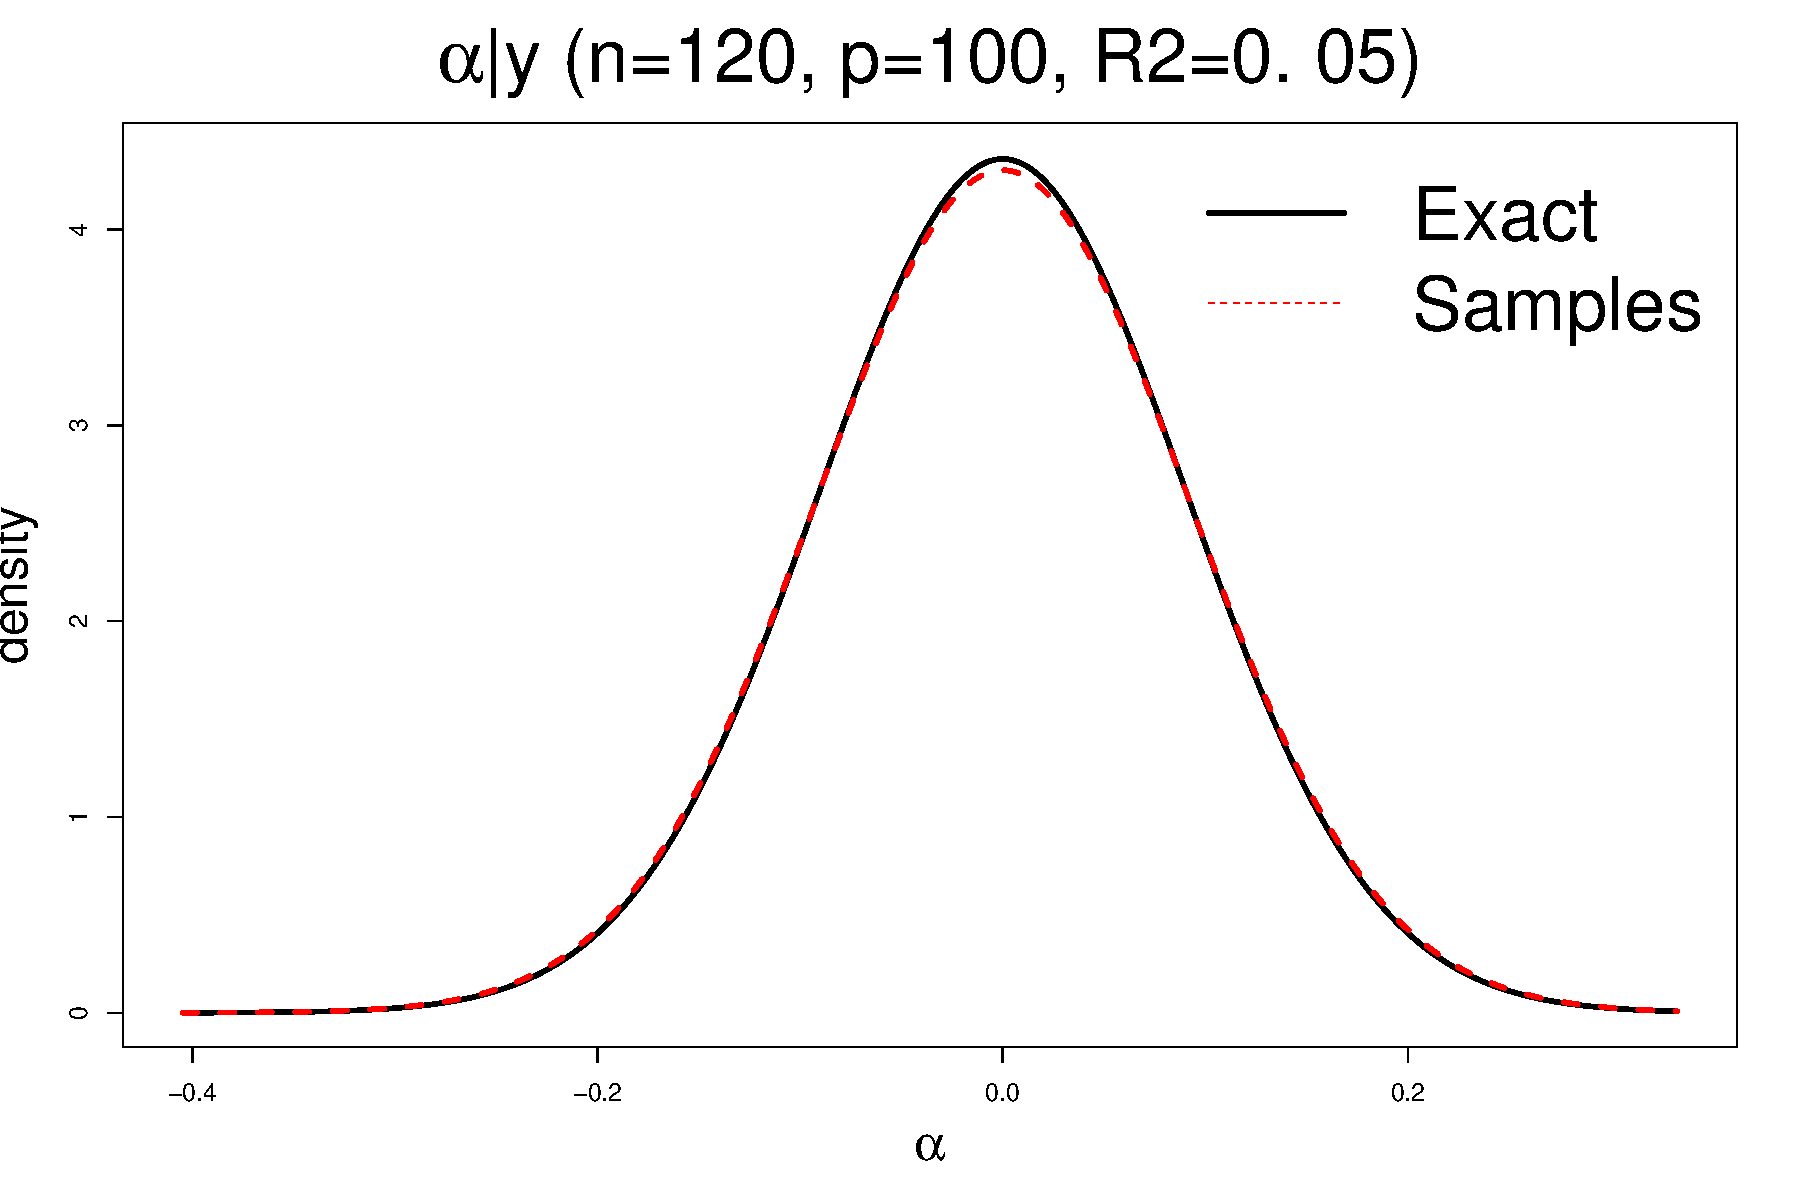
\includegraphics[scale=0.5]{code/alphaGivenY.pdf}
	\label{fig:alphaGivenY}
	\caption{The distribution of $\alpha | y$ for $n = 120$, $p = 3$, $20$ or $100$ and $R^2 = 0.05$ or $0.95$.}
\end{figure}

\begin{figure}
	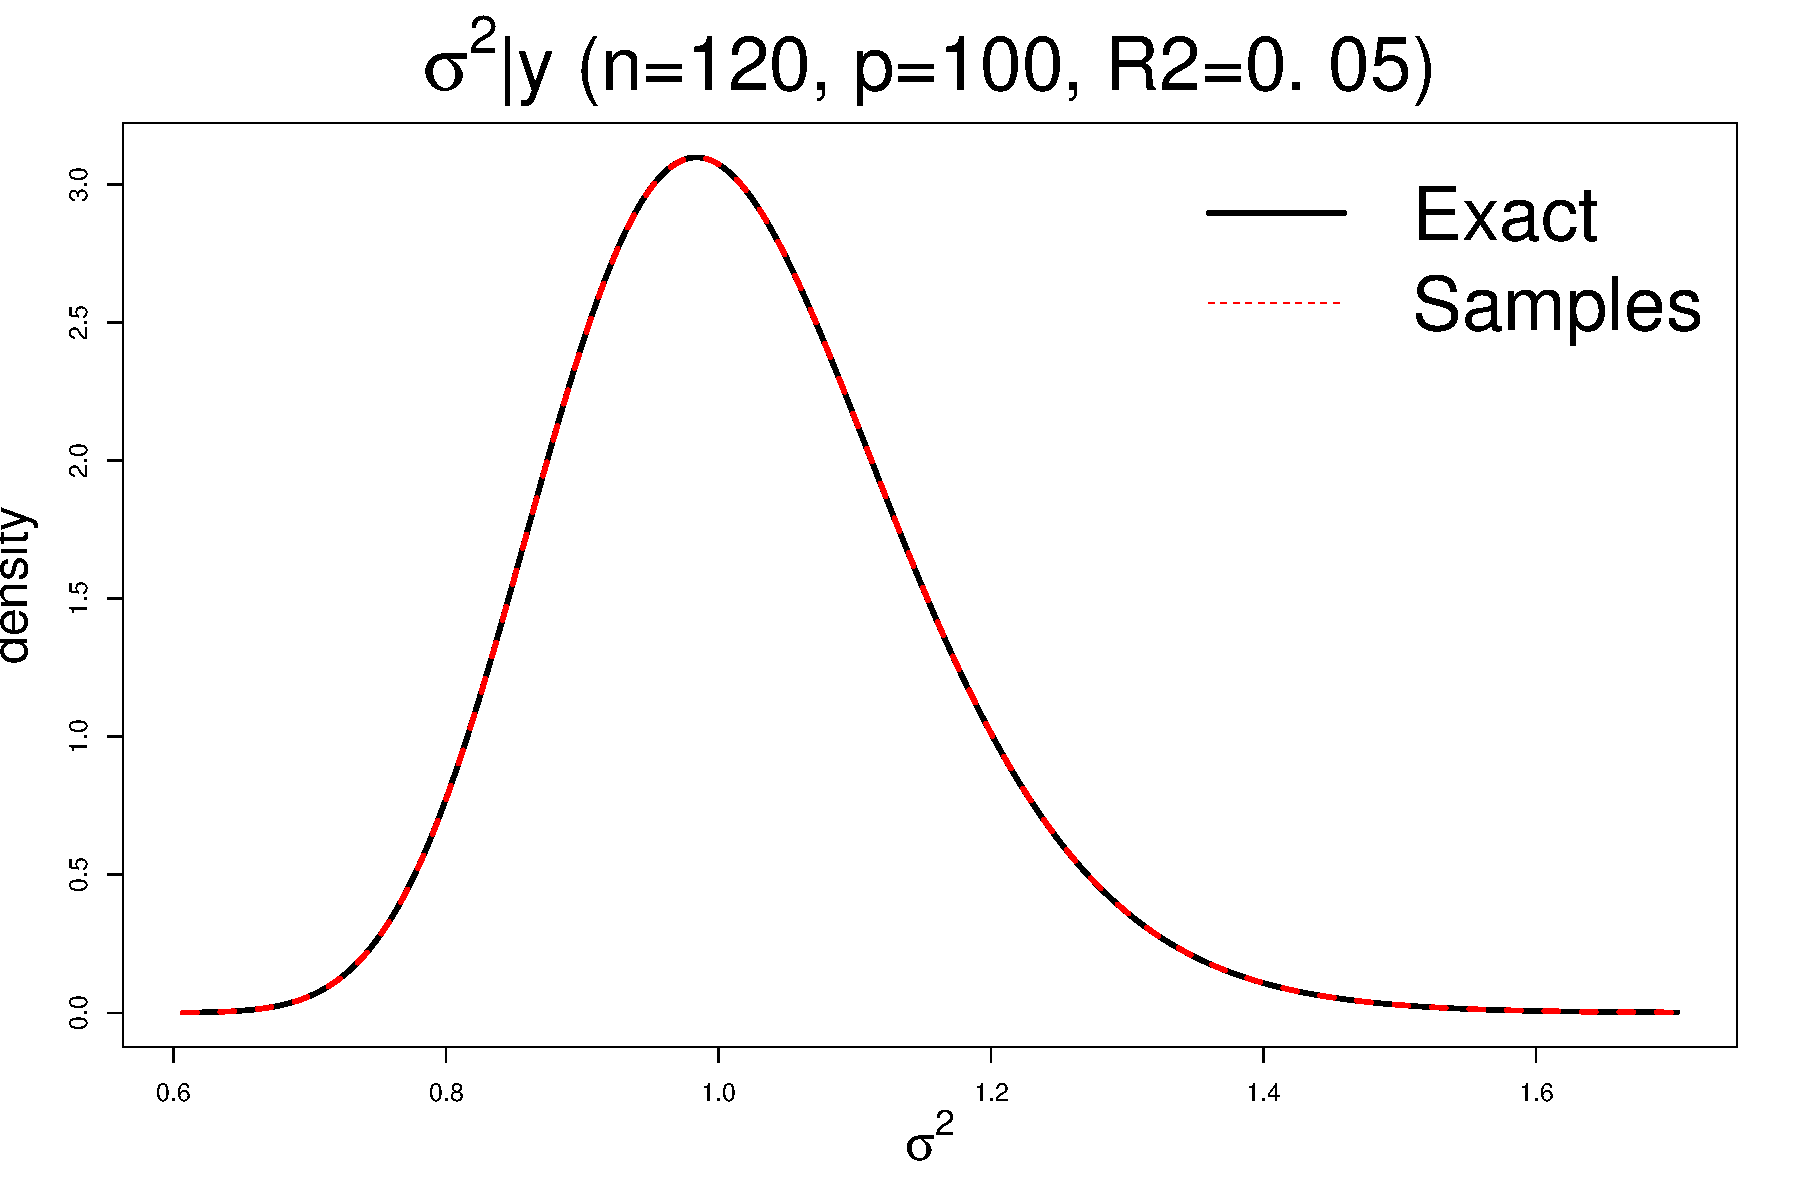
\includegraphics[scale=0.5]{code/sigma2GivenY.pdf}
	\label{fig:sigma2GivenY}
	\caption{The distribution of $\sigma^2 | y$ for $n = 120$, $p = 3$, $20$ or $100$ and $R^2 = 0.05$ or $0.95$.}
\end{figure}

\begin{figure}
	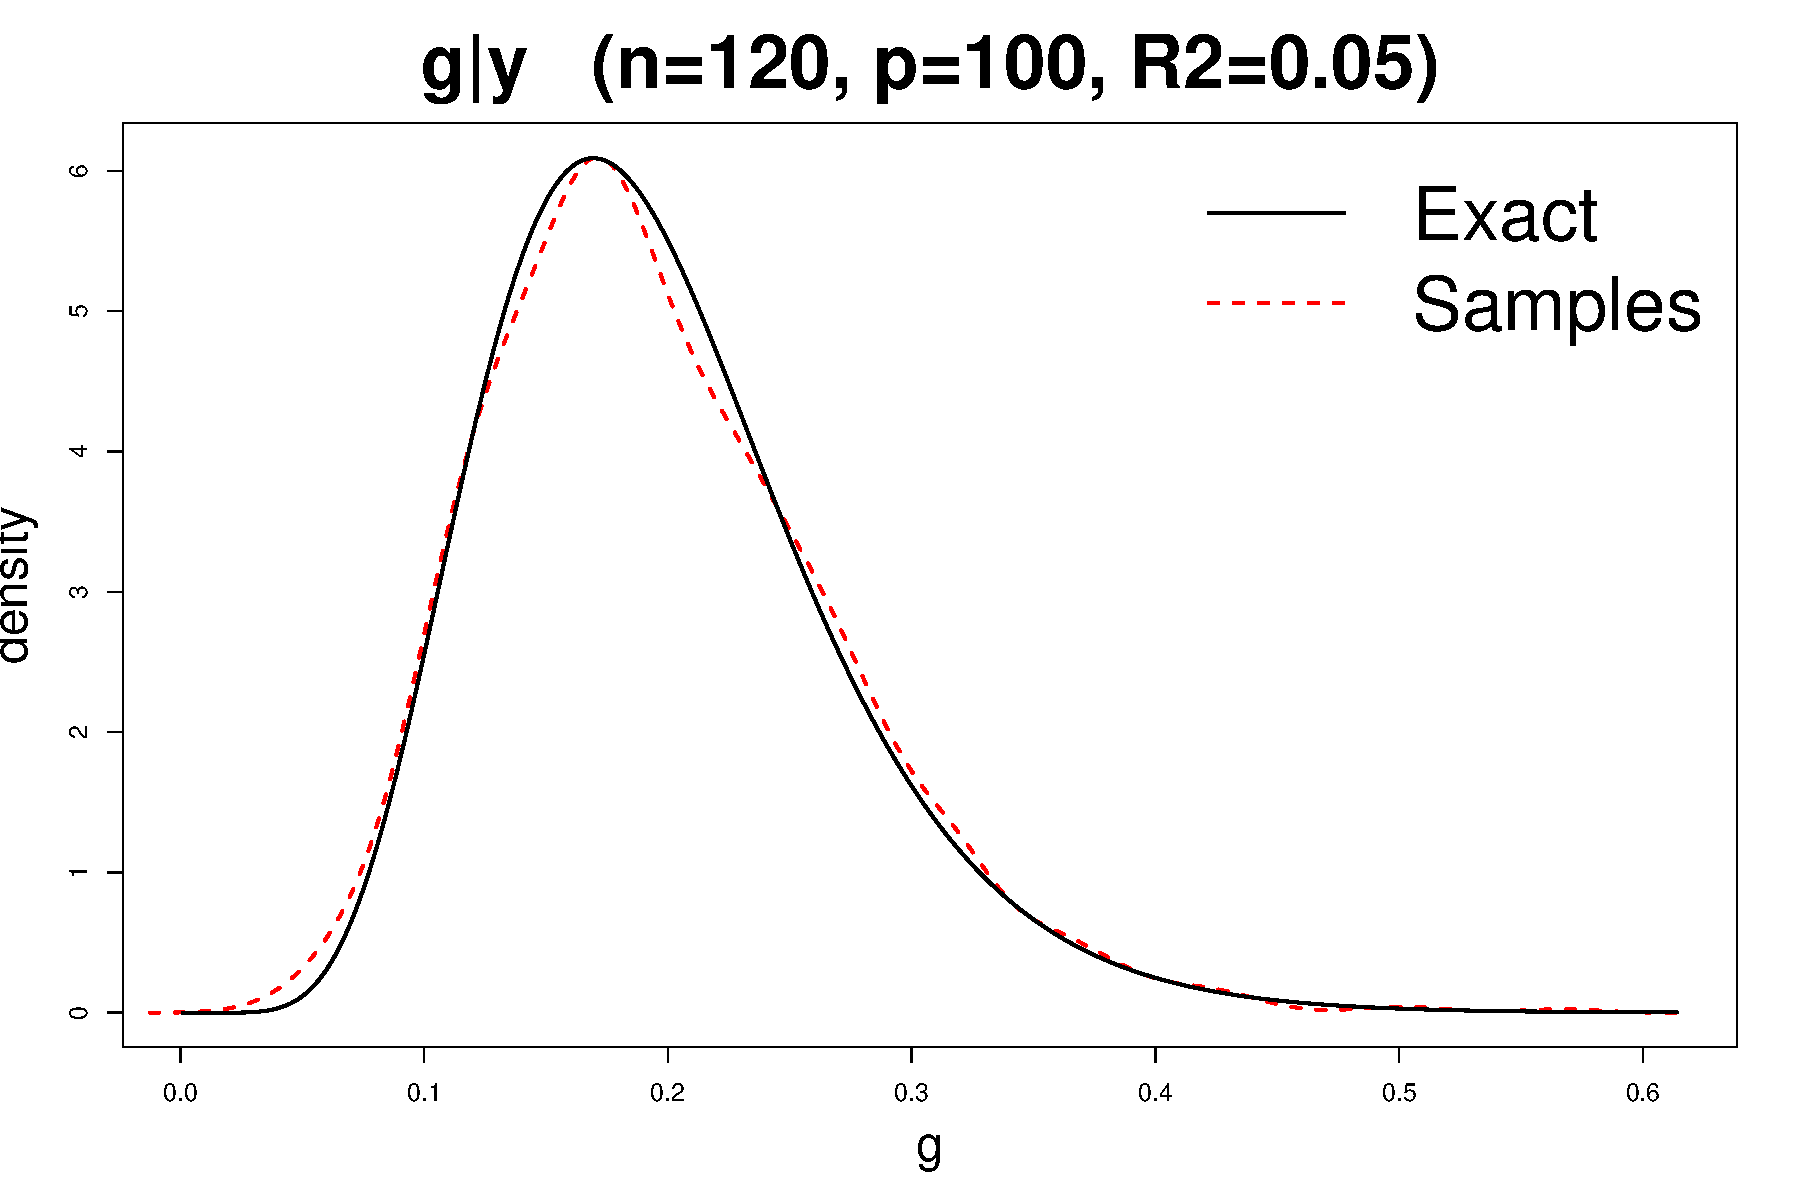
\includegraphics[scale=0.5]{code/gGivenY.pdf}
	\label{fig:gGivenY}
	\caption{The distribution of $g | y$ for $n = 120$, $p = 3$, $20$ or $100$ and $R^2 = 0.05$ or $0.95$,
					 when the prior on $g$ is the Beta Prime prior from \citep{Maruyama2011}.}
\end{figure}

\begin{figure}
	\includegraphics[scale=0.5]{code/BetaHitters.pdf}
	\label{fig:BetaHitters}
	\caption{The distribution of the regression co-efficient posteriors for the Hitters data set.}
\end{figure}


\subsection{Implementation details}
\label{sec:implementation}

We traverse the models in $\Gamma$ in Graycode order.
This ensures that as the algorithm moves from one model to another, only one covariate either enters or leaves
the model.
This allows us to use Rank-1 updates and downdates of $(\mX^\top \mX)^{-1}$ to greatly decrease the
computational cost of calculating $R_\vgamma^2$ from $\BigO(np^3)$ to $\BigO(np^2)$.
Special care was taken to minimise memory allocation and deallocation.
The \texttt{Rcpp} and \texttt{RcppEigen} libraries were used to ensure the implementation was performant.

Initially, $\vgamma = (1, 0, 0, \ldots, 0, 0)^\top$. So $(\mX_\vgamma^\top \mX_\vgamma)^{-1} =
(\vx_\vgamma^\top \vx_\vgamma)^{-1}$ which is a scalar, and so can be computed in $\BigO(n)$. Then the set of
possible models $\vgamma$ is iterated through in graycode order. This ensures that only one entry of $\vgamma$
changes as each model is visited, allowing the new $(\mX_\vgamma^\top \mX_\vgamma)^{-1}$ to be calculated
using the previous $(\mX_\vgamma^\top \mX_\vgamma)^{-1}$ and a rank-1 update. This allows us to avoid directly
computing the new $\mX_\vgamma^\top \mX_\vgamma$ and then performing a full inversion, reducing a $\BigO(n
p^3)$ operation to $\BigO(n p^2)$.

\mgc{Think about distribution of bit strings. What is the expectation of $p$? I think it's simply $p/2$}

\section{Conclusion and Discussion}
\label{sec:conclusion}

% This is all invalid now
The Variational Bayes approximation produces results which are almost identical to the exact likelihood.
The VB metholodology extends naturally to new situations, such as robust model fitting, mixed effects, missing
data, measurement error and splines. We are able to retain high accuracy with less computational overhead than
exact or MCMC.

All of the variational parameters in Algorithm \ref{alg:algorithm_two} except $\tau_g$ depend only on
$\tau_g$ and the fixed quantities $n$, $p$, $R^2$, $\mX$ and $\vy$. This allows us to optimise $\tau_g$
only, and then set the rest of the variational parameters at the end of the algorithm. The fact that only
univariate optimisation is required reduces the computation required to fit our approximation considerably,
which makes this algorithm applicable when speed and/or the ability to parallelise the algorithm are
paramount, such as model selection via structured Variational Bayes.

\appendix
\subsection{Useful Results}	

We first present the following results which will aid us in deriving the expressions required for fully Bayesian
inference over the parameters in the model.

\begin{equation}\label{res:01}
	\int \exp\left\{ -\tfrac{1}{2}\vx^T\mA\vx + \vb^T\vx \right\} d \vx = |2\pi\mSigma|^{1/2} \exp\left\{ \tfrac{1}{2}\vmu^T\mSigma^{-1}\vmu \right\}
\end{equation}
where $\vmu = \mA^{-1}\vb$ and $\mSigma = \mA^{-1}$.
 
If $\vone^T\vy=0$ the $R$-squared statistic can be expressed
\begin{equation} \label{res:02}
	R^2 = \frac{\vy^T\mX(\mX^T\mX)^{-1}\mX^T\vy}{\|\vy\|^2}
\end{equation}
where $R^2$ is the usual $R$-squared statistic associated with least squares regression.

Equation 3.194 (iii) of \citep{Gradshteyn1988} is
\begin{equation}\label{res:03}
	\int_0^\infty \frac{ x^{\mu - 1} }{(1 + \beta x)^\nu} dx = \beta^{-\mu} \mbox{Beta}(\mu,\nu - \mu) \quad \quad \mbox{(assuming $\mu,\nu>0$ and $\nu>\mu$).}
\end{equation}

Equation 3.385 of \citep{Gradshteyn1988} is
\begin{equation} \label{res:04}
	\int_{0}^1 x^{\nu - 1} (1 - x)^{\lambda - 1}(1 - \beta x)^{\varrho} e^{-\mu x} dx = \mbox{Beta}(\nu,\lambda) \Phi_1(\nu,\varrho,\lambda+\nu,-\mu,\beta)
\end{equation}

\noindent provided $\mbox{Re}(\lambda)>0$, $\mbox{Re}(\nu)>0$ and $|\mbox{arg}(1-\beta)|<\pi$.



\backmatter
\appendix

\bibliographystyle{elsarticle-harv}
\bibliography{references_mendeley}

\end{document}